\documentclass[twoside]{book}

% Packages required by doxygen
\usepackage{calc}
\usepackage{doxygen}
\usepackage{graphicx}
\usepackage[utf8]{inputenc}
\usepackage{makeidx}
\usepackage{multicol}
\usepackage{multirow}
\usepackage{textcomp}
\usepackage[table]{xcolor}

% Font selection
\usepackage[T1]{fontenc}
\usepackage{mathptmx}
\usepackage[scaled=.90]{helvet}
\usepackage{courier}
\usepackage{amssymb}
\usepackage{sectsty}
\renewcommand{\familydefault}{\sfdefault}
\allsectionsfont{%
  \fontseries{bc}\selectfont%
  \color{darkgray}%
}
\renewcommand{\DoxyLabelFont}{%
  \fontseries{bc}\selectfont%
  \color{darkgray}%
}

% Page & text layout
\usepackage{geometry}
\geometry{%
  a4paper,%
  top=2.5cm,%
  bottom=2.5cm,%
  left=2.5cm,%
  right=2.5cm%
}
\tolerance=750
\hfuzz=15pt
\hbadness=750
\setlength{\emergencystretch}{15pt}
\setlength{\parindent}{0cm}
\setlength{\parskip}{0.2cm}
\makeatletter
\renewcommand{\paragraph}{%
  \@startsection{paragraph}{4}{0ex}{-1.0ex}{1.0ex}{%
    \normalfont\normalsize\bfseries\SS@parafont%
  }%
}
\renewcommand{\subparagraph}{%
  \@startsection{subparagraph}{5}{0ex}{-1.0ex}{1.0ex}{%
    \normalfont\normalsize\bfseries\SS@subparafont%
  }%
}
\makeatother

% Headers & footers
\usepackage{fancyhdr}
\pagestyle{fancyplain}
\fancyhead[LE]{\fancyplain{}{\bfseries\thepage}}
\fancyhead[CE]{\fancyplain{}{}}
\fancyhead[RE]{\fancyplain{}{\bfseries\leftmark}}
\fancyhead[LO]{\fancyplain{}{\bfseries\rightmark}}
\fancyhead[CO]{\fancyplain{}{}}
\fancyhead[RO]{\fancyplain{}{\bfseries\thepage}}
\fancyfoot[LE]{\fancyplain{}{}}
\fancyfoot[CE]{\fancyplain{}{}}
\fancyfoot[RE]{\fancyplain{}{\bfseries\scriptsize Generated on Sun May 24 2015 17\-:39\-:04 for 42sh by Doxygen }}
\fancyfoot[LO]{\fancyplain{}{\bfseries\scriptsize Generated on Sun May 24 2015 17\-:39\-:04 for 42sh by Doxygen }}
\fancyfoot[CO]{\fancyplain{}{}}
\fancyfoot[RO]{\fancyplain{}{}}
\renewcommand{\footrulewidth}{0.4pt}
\renewcommand{\chaptermark}[1]{%
  \markboth{#1}{}%
}
\renewcommand{\sectionmark}[1]{%
  \markright{\thesection\ #1}%
}

% Indices & bibliography
\usepackage{natbib}
\usepackage[titles]{tocloft}
\setcounter{tocdepth}{3}
\setcounter{secnumdepth}{5}
\makeindex

% Custom commands
\newcommand{\clearemptydoublepage}{%
  \newpage{\pagestyle{empty}\cleardoublepage}%
}


%===== C O N T E N T S =====

\begin{document}

% Titlepage & ToC
\pagenumbering{roman}
\begin{titlepage}
\vspace*{7cm}
\begin{center}%
{\Large 42sh \\[1ex]\large 3.\-0 }\\
\vspace*{1cm}
{\large Generated by Doxygen 1.8.5}\\
\vspace*{0.5cm}
{\small Sun May 24 2015 17:39:04}\\
\end{center}
\end{titlepage}
\clearemptydoublepage
\tableofcontents
\clearemptydoublepage
\pagenumbering{arabic}

%--- Begin generated contents ---
\chapter{Data Structure Index}
\section{Data Structures}
Here are the data structures with brief descriptions\-:\begin{DoxyCompactList}
\item\contentsline{section}{{\bf s\-\_\-alias} }{\pageref{structs__alias}}{}
\item\contentsline{section}{{\bf s\-\_\-bref} }{\pageref{structs__bref}}{}
\item\contentsline{section}{{\bf s\-\_\-cmd} }{\pageref{structs__cmd}}{}
\item\contentsline{section}{{\bf s\-\_\-cmds} }{\pageref{structs__cmds}}{}
\item\contentsline{section}{{\bf s\-\_\-data} }{\pageref{structs__data}}{}
\item\contentsline{section}{{\bf s\-\_\-format} }{\pageref{structs__format}}{}
\item\contentsline{section}{{\bf s\-\_\-history} }{\pageref{structs__history}}{}
\item\contentsline{section}{{\bf s\-\_\-list} }{\pageref{structs__list}}{}
\item\contentsline{section}{{\bf s\-\_\-list\-\_\-line} }{\pageref{structs__list__line}}{}
\item\contentsline{section}{{\bf s\-\_\-stock} }{\pageref{structs__stock}}{}
\end{DoxyCompactList}

\chapter{File Index}
\section{File List}
Here is a list of all files with brief descriptions\-:\begin{DoxyCompactList}
\item\contentsline{section}{alias/{\bf alias.\-c} }{\pageref{alias_8c}}{}
\item\contentsline{section}{alias/{\bf alias\-\_\-etc.\-c} }{\pageref{alias__etc_8c}}{}
\item\contentsline{section}{alias/{\bf gnl.\-c} }{\pageref{gnl_8c}}{}
\item\contentsline{section}{alias/{\bf pars\-\_\-alias.\-c} }{\pageref{pars__alias_8c}}{}
\item\contentsline{section}{alias/{\bf str\-\_\-cat.\-c} }{\pageref{str__cat_8c}}{}
\item\contentsline{section}{auto\-\_\-complete/{\bf auto\-\_\-complete.\-c} }{\pageref{auto__complete_8c}}{}
\item\contentsline{section}{auto\-\_\-complete/{\bf functions\-\_\-complete.\-c} }{\pageref{functions__complete_8c}}{}
\item\contentsline{section}{builtin/{\bf builtin.\-c} }{\pageref{builtin_8c}}{}
\item\contentsline{section}{builtin/{\bf cd.\-c} }{\pageref{cd_8c}}{}
\item\contentsline{section}{builtin/{\bf forbuiltin.\-c} }{\pageref{forbuiltin_8c}}{}
\item\contentsline{section}{builtin/{\bf getvar.\-c} }{\pageref{getvar_8c}}{}
\item\contentsline{section}{builtin/{\bf top\-\_\-builtin.\-c} }{\pageref{top__builtin_8c}}{}
\item\contentsline{section}{builtin/{\bf utils.\-c} }{\pageref{builtin_2utils_8c}}{}
\item\contentsline{section}{exe/{\bf default\-\_\-path.\-c} }{\pageref{default__path_8c}}{}
\item\contentsline{section}{exe/{\bf exe\-\_\-cmd.\-c} }{\pageref{exe__cmd_8c}}{}
\item\contentsline{section}{exe/{\bf is\-\_\-builtin.\-c} }{\pageref{is__builtin_8c}}{}
\item\contentsline{section}{exe/{\bf pipe.\-c} }{\pageref{pipe_8c}}{}
\item\contentsline{section}{exe/{\bf redirection\-\_\-left.\-c} }{\pageref{redirection__left_8c}}{}
\item\contentsline{section}{exe/{\bf redirection\-\_\-right.\-c} }{\pageref{redirection__right_8c}}{}
\item\contentsline{section}{glob/{\bf glob.\-c} }{\pageref{glob_8c}}{}
\item\contentsline{section}{glob/{\bf stars.\-c} }{\pageref{stars_8c}}{}
\item\contentsline{section}{include/{\bf builtin.\-h} }{\pageref{builtin_8h}}{}
\item\contentsline{section}{include/{\bf get\-\_\-next\-\_\-line.\-h} }{\pageref{get__next__line_8h}}{}
\item\contentsline{section}{include/{\bf lib.\-h} }{\pageref{lib_8h}}{}
\item\contentsline{section}{include/{\bf ps1.\-h} }{\pageref{ps1_8h}}{}
\item\contentsline{section}{include/{\bf shell.\-h} }{\pageref{shell_8h}}{}
\item\contentsline{section}{lib/my/{\bf get\-\_\-next\-\_\-line.\-c} }{\pageref{get__next__line_8c}}{}
\item\contentsline{section}{lib/my/{\bf len\-\_\-tab.\-c} }{\pageref{len__tab_8c}}{}
\item\contentsline{section}{lib/my/{\bf malloc\-\_\-str.\-c} }{\pageref{malloc__str_8c}}{}
\item\contentsline{section}{lib/my/{\bf my\-\_\-getnbr.\-c} }{\pageref{my__getnbr_8c}}{}
\item\contentsline{section}{lib/my/{\bf my\-\_\-put\-\_\-nbr.\-c} }{\pageref{my__put__nbr_8c}}{}
\item\contentsline{section}{lib/my/{\bf my\-\_\-putchar.\-c} }{\pageref{my__putchar_8c}}{}
\item\contentsline{section}{lib/my/{\bf my\-\_\-putstr.\-c} }{\pageref{my__putstr_8c}}{}
\item\contentsline{section}{lib/my/{\bf my\-\_\-strcat.\-c} }{\pageref{my__strcat_8c}}{}
\item\contentsline{section}{lib/my/{\bf my\-\_\-strcat\-\_\-from.\-c} }{\pageref{my__strcat__from_8c}}{}
\item\contentsline{section}{lib/my/{\bf my\-\_\-strcmp.\-c} }{\pageref{my__strcmp_8c}}{}
\item\contentsline{section}{lib/my/{\bf my\-\_\-strcpy.\-c} }{\pageref{my__strcpy_8c}}{}
\item\contentsline{section}{lib/my/{\bf my\-\_\-strcpy\-\_\-from.\-c} }{\pageref{my__strcpy__from_8c}}{}
\item\contentsline{section}{lib/my/{\bf my\-\_\-strdup.\-c} }{\pageref{my__strdup_8c}}{}
\item\contentsline{section}{lib/my/{\bf my\-\_\-strlen.\-c} }{\pageref{my__strlen_8c}}{}
\item\contentsline{section}{lib/my/{\bf my\-\_\-strncat.\-c} }{\pageref{my__strncat_8c}}{}
\item\contentsline{section}{lib/my/{\bf my\-\_\-strncmp.\-c} }{\pageref{my__strncmp_8c}}{}
\item\contentsline{section}{lib/my/{\bf my\-\_\-strncpy.\-c} }{\pageref{my__strncpy_8c}}{}
\item\contentsline{section}{lib/my/{\bf my\-\_\-strndup.\-c} }{\pageref{my__strndup_8c}}{}
\item\contentsline{section}{lib/my/{\bf str\-\_\-to\-\_\-word\-\_\-tab.\-c} }{\pageref{str__to__word__tab_8c}}{}
\item\contentsline{section}{parsing/{\bf parsing\-\_\-cmd.\-c} }{\pageref{parsing__cmd_8c}}{}
\item\contentsline{section}{parsing/{\bf parsing\-\_\-general.\-c} }{\pageref{parsing__general_8c}}{}
\item\contentsline{section}{parsing/{\bf parsing\-\_\-pipe.\-c} }{\pageref{parsing__pipe_8c}}{}
\item\contentsline{section}{parsing/{\bf parsing\-\_\-tilde.\-c} }{\pageref{parsing__tilde_8c}}{}
\item\contentsline{section}{parsing/{\bf redirection.\-c} }{\pageref{redirection_8c}}{}
\item\contentsline{section}{prompt\-\_\-read\-\_\-termcaps/{\bf clean\-\_\-screen.\-c} }{\pageref{clean__screen_8c}}{}
\item\contentsline{section}{prompt\-\_\-read\-\_\-termcaps/{\bf clear\-\_\-line.\-c} }{\pageref{clear__line_8c}}{}
\item\contentsline{section}{prompt\-\_\-read\-\_\-termcaps/{\bf gere\-\_\-key.\-c} }{\pageref{gere__key_8c}}{}
\item\contentsline{section}{prompt\-\_\-read\-\_\-termcaps/{\bf init.\-c} }{\pageref{init_8c}}{}
\item\contentsline{section}{prompt\-\_\-read\-\_\-termcaps/{\bf insert\-\_\-list\-\_\-double.\-c} }{\pageref{insert__list__double_8c}}{}
\item\contentsline{section}{prompt\-\_\-read\-\_\-termcaps/{\bf last\-\_\-word.\-c} }{\pageref{last__word_8c}}{}
\item\contentsline{section}{prompt\-\_\-read\-\_\-termcaps/{\bf loop\-\_\-read.\-c} }{\pageref{loop__read_8c}}{}
\item\contentsline{section}{prompt\-\_\-read\-\_\-termcaps/{\bf modif\-\_\-cmd.\-c} }{\pageref{modif__cmd_8c}}{}
\item\contentsline{section}{prompt\-\_\-read\-\_\-termcaps/{\bf move.\-c} }{\pageref{move_8c}}{}
\item\contentsline{section}{prompt\-\_\-read\-\_\-termcaps/{\bf print\-\_\-cursor.\-c} }{\pageref{print__cursor_8c}}{}
\item\contentsline{section}{prompt\-\_\-read\-\_\-termcaps/{\bf prompt\-\_\-dyn.\-c} }{\pageref{prompt__dyn_8c}}{}
\item\contentsline{section}{ps1/{\bf tab\-\_\-fonc.\-c} }{\pageref{tab__fonc_8c}}{}
\item\contentsline{section}{ps1/{\bf utils.\-c} }{\pageref{ps1_2utils_8c}}{}
\end{DoxyCompactList}

\chapter{Data Structure Documentation}
\section{s\-\_\-alias Struct Reference}
\label{structs__alias}\index{s\-\_\-alias@{s\-\_\-alias}}


{\ttfamily \#include $<$shell.\-h$>$}



Collaboration diagram for s\-\_\-alias\-:\nopagebreak
\begin{figure}[H]
\begin{center}
\leavevmode
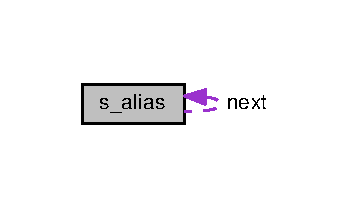
\includegraphics[width=168pt]{structs__alias__coll__graph}
\end{center}
\end{figure}
\subsection*{Data Fields}
\begin{DoxyCompactItemize}
\item 
char $\ast$ {\bf old}
\item 
char $\ast$ {\bf new}
\item 
struct {\bf s\-\_\-alias} $\ast$ {\bf next}
\end{DoxyCompactItemize}


\subsection{Detailed Description}


Definition at line 17 of file shell.\-h.



\subsection{Field Documentation}
\index{s\-\_\-alias@{s\-\_\-alias}!new@{new}}
\index{new@{new}!s_alias@{s\-\_\-alias}}
\subsubsection[{new}]{\setlength{\rightskip}{0pt plus 5cm}char$\ast$ new}\label{structs__alias_a80de185e58c66866a3e560697b9fb978}


Definition at line 20 of file shell.\-h.

\index{s\-\_\-alias@{s\-\_\-alias}!next@{next}}
\index{next@{next}!s_alias@{s\-\_\-alias}}
\subsubsection[{next}]{\setlength{\rightskip}{0pt plus 5cm}struct {\bf s\-\_\-alias}$\ast$ next}\label{structs__alias_a228d8745e3b5e095fe1a256c236a8d9a}


Definition at line 21 of file shell.\-h.

\index{s\-\_\-alias@{s\-\_\-alias}!old@{old}}
\index{old@{old}!s_alias@{s\-\_\-alias}}
\subsubsection[{old}]{\setlength{\rightskip}{0pt plus 5cm}char$\ast$ old}\label{structs__alias_a32487cbad62d1e9a7ea00010f5dc58bb}


Definition at line 19 of file shell.\-h.



The documentation for this struct was generated from the following file\-:\begin{DoxyCompactItemize}
\item 
include/{\bf shell.\-h}\end{DoxyCompactItemize}

\section{s\-\_\-bref Struct Reference}
\label{structs__bref}\index{s\-\_\-bref@{s\-\_\-bref}}


{\ttfamily \#include $<$builtin.\-h$>$}

\subsection*{Data Fields}
\begin{DoxyCompactItemize}
\item 
char $\ast$ {\bf ref}
\item 
int($\ast$ {\bf builtin} )(char $\ast$$\ast$, {\bf t\-\_\-data} $\ast$)
\end{DoxyCompactItemize}


\subsection{Detailed Description}


Definition at line 22 of file builtin.\-h.



\subsection{Field Documentation}
\index{s\-\_\-bref@{s\-\_\-bref}!builtin@{builtin}}
\index{builtin@{builtin}!s_bref@{s\-\_\-bref}}
\subsubsection[{builtin}]{\setlength{\rightskip}{0pt plus 5cm}int($\ast$ builtin)(char $\ast$$\ast$, {\bf t\-\_\-data} $\ast$)}\label{structs__bref_a3cffecc657840bcfdbd40bfaf96be9d5}


Definition at line 25 of file builtin.\-h.

\index{s\-\_\-bref@{s\-\_\-bref}!ref@{ref}}
\index{ref@{ref}!s_bref@{s\-\_\-bref}}
\subsubsection[{ref}]{\setlength{\rightskip}{0pt plus 5cm}char$\ast$ ref}\label{structs__bref_a409d98460fccb0c31bf8887117e68f36}


Definition at line 24 of file builtin.\-h.



The documentation for this struct was generated from the following file\-:\begin{DoxyCompactItemize}
\item 
include/{\bf builtin.\-h}\end{DoxyCompactItemize}

\section{s\-\_\-cmd Struct Reference}
\label{structs__cmd}\index{s\-\_\-cmd@{s\-\_\-cmd}}


{\ttfamily \#include $<$shell.\-h$>$}



Collaboration diagram for s\-\_\-cmd\-:\nopagebreak
\begin{figure}[H]
\begin{center}
\leavevmode
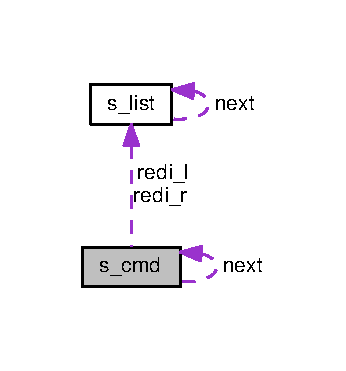
\includegraphics[width=166pt]{structs__cmd__coll__graph}
\end{center}
\end{figure}
\subsection*{Data Fields}
\begin{DoxyCompactItemize}
\item 
char $\ast$$\ast$ {\bf tab}
\item 
{\bf t\-\_\-list} $\ast$ {\bf redi\-\_\-r}
\item 
{\bf t\-\_\-list} $\ast$ {\bf redi\-\_\-l}
\item 
struct {\bf s\-\_\-cmd} $\ast$ {\bf next}
\end{DoxyCompactItemize}


\subsection{Detailed Description}


Definition at line 37 of file shell.\-h.



\subsection{Field Documentation}
\index{s\-\_\-cmd@{s\-\_\-cmd}!next@{next}}
\index{next@{next}!s_cmd@{s\-\_\-cmd}}
\subsubsection[{next}]{\setlength{\rightskip}{0pt plus 5cm}struct {\bf s\-\_\-cmd}$\ast$ next}\label{structs__cmd_aadb06044d2e679ed4395a2680dc6962a}


Definition at line 42 of file shell.\-h.

\index{s\-\_\-cmd@{s\-\_\-cmd}!redi\-\_\-l@{redi\-\_\-l}}
\index{redi\-\_\-l@{redi\-\_\-l}!s_cmd@{s\-\_\-cmd}}
\subsubsection[{redi\-\_\-l}]{\setlength{\rightskip}{0pt plus 5cm}{\bf t\-\_\-list}$\ast$ redi\-\_\-l}\label{structs__cmd_a3eb86f4753299ed84389481f46694140}


Definition at line 41 of file shell.\-h.

\index{s\-\_\-cmd@{s\-\_\-cmd}!redi\-\_\-r@{redi\-\_\-r}}
\index{redi\-\_\-r@{redi\-\_\-r}!s_cmd@{s\-\_\-cmd}}
\subsubsection[{redi\-\_\-r}]{\setlength{\rightskip}{0pt plus 5cm}{\bf t\-\_\-list}$\ast$ redi\-\_\-r}\label{structs__cmd_a8629d9a24e605fcc6a82b55b1a870a07}


Definition at line 40 of file shell.\-h.

\index{s\-\_\-cmd@{s\-\_\-cmd}!tab@{tab}}
\index{tab@{tab}!s_cmd@{s\-\_\-cmd}}
\subsubsection[{tab}]{\setlength{\rightskip}{0pt plus 5cm}char$\ast$$\ast$ tab}\label{structs__cmd_a095ef5f32e2dd3c36f801fc514372ee3}


Definition at line 39 of file shell.\-h.



The documentation for this struct was generated from the following file\-:\begin{DoxyCompactItemize}
\item 
include/{\bf shell.\-h}\end{DoxyCompactItemize}

\section{s\-\_\-cmds Struct Reference}
\label{structs__cmds}\index{s\-\_\-cmds@{s\-\_\-cmds}}


{\ttfamily \#include $<$shell.\-h$>$}



Collaboration diagram for s\-\_\-cmds\-:\nopagebreak
\begin{figure}[H]
\begin{center}
\leavevmode
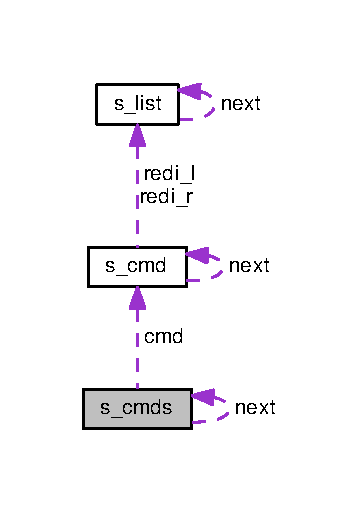
\includegraphics[width=172pt]{structs__cmds__coll__graph}
\end{center}
\end{figure}
\subsection*{Data Fields}
\begin{DoxyCompactItemize}
\item 
{\bf t\-\_\-cmd} $\ast$ {\bf cmd}
\item 
char {\bf sep}
\item 
struct {\bf s\-\_\-cmds} $\ast$ {\bf next}
\end{DoxyCompactItemize}


\subsection{Detailed Description}


Definition at line 45 of file shell.\-h.



\subsection{Field Documentation}
\index{s\-\_\-cmds@{s\-\_\-cmds}!cmd@{cmd}}
\index{cmd@{cmd}!s_cmds@{s\-\_\-cmds}}
\subsubsection[{cmd}]{\setlength{\rightskip}{0pt plus 5cm}{\bf t\-\_\-cmd}$\ast$ cmd}\label{structs__cmds_a7833a1c1c3d06a0dc2ef489abda7bf64}


Definition at line 47 of file shell.\-h.

\index{s\-\_\-cmds@{s\-\_\-cmds}!next@{next}}
\index{next@{next}!s_cmds@{s\-\_\-cmds}}
\subsubsection[{next}]{\setlength{\rightskip}{0pt plus 5cm}struct {\bf s\-\_\-cmds}$\ast$ next}\label{structs__cmds_a0025c4bc6dd26be6d05df24de3a1ae88}


Definition at line 49 of file shell.\-h.

\index{s\-\_\-cmds@{s\-\_\-cmds}!sep@{sep}}
\index{sep@{sep}!s_cmds@{s\-\_\-cmds}}
\subsubsection[{sep}]{\setlength{\rightskip}{0pt plus 5cm}char sep}\label{structs__cmds_a2f44b091be60ccdd664997eb163d2ff4}


Definition at line 48 of file shell.\-h.



The documentation for this struct was generated from the following file\-:\begin{DoxyCompactItemize}
\item 
include/{\bf shell.\-h}\end{DoxyCompactItemize}

\section{s\-\_\-data Struct Reference}
\label{structs__data}\index{s\-\_\-data@{s\-\_\-data}}


{\ttfamily \#include $<$shell.\-h$>$}



Collaboration diagram for s\-\_\-data\-:\nopagebreak
\begin{figure}[H]
\begin{center}
\leavevmode
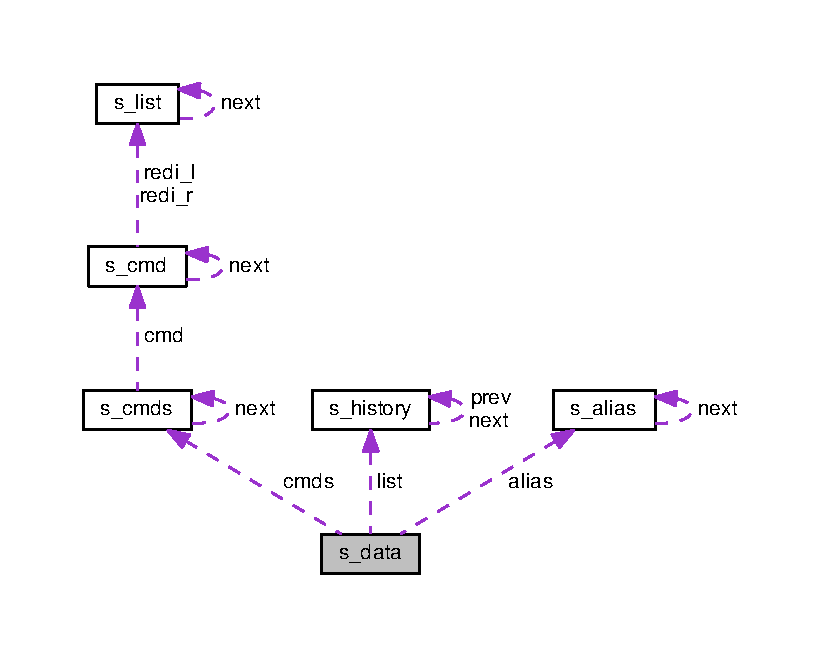
\includegraphics[width=350pt]{structs__data__coll__graph}
\end{center}
\end{figure}
\subsection*{Data Fields}
\begin{DoxyCompactItemize}
\item 
int {\bf dynam\-\_\-prompt}
\item 
{\bf t\-\_\-alias} $\ast$ {\bf alias}
\item 
{\bf t\-\_\-cmds} $\ast$ {\bf cmds}
\item 
char $\ast$$\ast$ {\bf env}
\item 
char $\ast$ {\bf ps1}
\item 
int {\bf return\-\_\-exe}
\item 
int {\bf return\-\_\-exit}
\item 
{\bf t\-\_\-history} $\ast$ {\bf list}
\end{DoxyCompactItemize}


\subsection{Detailed Description}


Definition at line 66 of file shell.\-h.



\subsection{Field Documentation}
\index{s\-\_\-data@{s\-\_\-data}!alias@{alias}}
\index{alias@{alias}!s_data@{s\-\_\-data}}
\subsubsection[{alias}]{\setlength{\rightskip}{0pt plus 5cm}{\bf t\-\_\-alias}$\ast$ alias}\label{structs__data_a605d498106be2e521c13025a71deb7ba}


Definition at line 69 of file shell.\-h.

\index{s\-\_\-data@{s\-\_\-data}!cmds@{cmds}}
\index{cmds@{cmds}!s_data@{s\-\_\-data}}
\subsubsection[{cmds}]{\setlength{\rightskip}{0pt plus 5cm}{\bf t\-\_\-cmds}$\ast$ cmds}\label{structs__data_afcffbc0c123dbca7c984b936e58c976b}


Definition at line 70 of file shell.\-h.

\index{s\-\_\-data@{s\-\_\-data}!dynam\-\_\-prompt@{dynam\-\_\-prompt}}
\index{dynam\-\_\-prompt@{dynam\-\_\-prompt}!s_data@{s\-\_\-data}}
\subsubsection[{dynam\-\_\-prompt}]{\setlength{\rightskip}{0pt plus 5cm}int dynam\-\_\-prompt}\label{structs__data_abf3d90c932142f8b97a4757ddec92fb1}


Definition at line 68 of file shell.\-h.

\index{s\-\_\-data@{s\-\_\-data}!env@{env}}
\index{env@{env}!s_data@{s\-\_\-data}}
\subsubsection[{env}]{\setlength{\rightskip}{0pt plus 5cm}char$\ast$$\ast$ env}\label{structs__data_a45c1547b79d23d508a01a427c3171ca4}


Definition at line 71 of file shell.\-h.

\index{s\-\_\-data@{s\-\_\-data}!list@{list}}
\index{list@{list}!s_data@{s\-\_\-data}}
\subsubsection[{list}]{\setlength{\rightskip}{0pt plus 5cm}{\bf t\-\_\-history}$\ast$ list}\label{structs__data_a1f8c1ae59fa5c273cd528969d4ba8dd7}


Definition at line 75 of file shell.\-h.

\index{s\-\_\-data@{s\-\_\-data}!ps1@{ps1}}
\index{ps1@{ps1}!s_data@{s\-\_\-data}}
\subsubsection[{ps1}]{\setlength{\rightskip}{0pt plus 5cm}char$\ast$ ps1}\label{structs__data_acfb34a195b82ba94df86b2ff75a18647}


Definition at line 72 of file shell.\-h.

\index{s\-\_\-data@{s\-\_\-data}!return\-\_\-exe@{return\-\_\-exe}}
\index{return\-\_\-exe@{return\-\_\-exe}!s_data@{s\-\_\-data}}
\subsubsection[{return\-\_\-exe}]{\setlength{\rightskip}{0pt plus 5cm}int return\-\_\-exe}\label{structs__data_a57883f7329f18bee1eae1d5589bdd2ec}


Definition at line 73 of file shell.\-h.

\index{s\-\_\-data@{s\-\_\-data}!return\-\_\-exit@{return\-\_\-exit}}
\index{return\-\_\-exit@{return\-\_\-exit}!s_data@{s\-\_\-data}}
\subsubsection[{return\-\_\-exit}]{\setlength{\rightskip}{0pt plus 5cm}int return\-\_\-exit}\label{structs__data_ac031cf6c1b18f3f224e088dd3a13b680}


Definition at line 74 of file shell.\-h.



The documentation for this struct was generated from the following file\-:\begin{DoxyCompactItemize}
\item 
include/{\bf shell.\-h}\end{DoxyCompactItemize}

\section{s\-\_\-format Struct Reference}
\label{structs__format}\index{s\-\_\-format@{s\-\_\-format}}


{\ttfamily \#include $<$ps1.\-h$>$}

\subsection*{Data Fields}
\begin{DoxyCompactItemize}
\item 
char {\bf format}
\item 
void($\ast$ {\bf ptr\-\_\-tab} )(char $\ast$$\ast$env)
\end{DoxyCompactItemize}


\subsection{Detailed Description}


Definition at line 22 of file ps1.\-h.



\subsection{Field Documentation}
\index{s\-\_\-format@{s\-\_\-format}!format@{format}}
\index{format@{format}!s_format@{s\-\_\-format}}
\subsubsection[{format}]{\setlength{\rightskip}{0pt plus 5cm}char format}\label{structs__format_a32fcb6024930af1ae33392a753c59679}


Definition at line 24 of file ps1.\-h.

\index{s\-\_\-format@{s\-\_\-format}!ptr\-\_\-tab@{ptr\-\_\-tab}}
\index{ptr\-\_\-tab@{ptr\-\_\-tab}!s_format@{s\-\_\-format}}
\subsubsection[{ptr\-\_\-tab}]{\setlength{\rightskip}{0pt plus 5cm}void($\ast$ ptr\-\_\-tab)(char $\ast$$\ast$env)}\label{structs__format_a821d5bfc90f45a86fe06458eca0f3f1e}


Definition at line 25 of file ps1.\-h.



The documentation for this struct was generated from the following file\-:\begin{DoxyCompactItemize}
\item 
include/{\bf ps1.\-h}\end{DoxyCompactItemize}

\section{s\-\_\-history Struct Reference}
\label{structs__history}\index{s\-\_\-history@{s\-\_\-history}}


{\ttfamily \#include $<$shell.\-h$>$}



Collaboration diagram for s\-\_\-history\-:\nopagebreak
\begin{figure}[H]
\begin{center}
\leavevmode
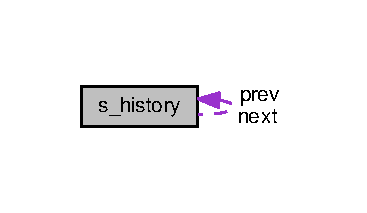
\includegraphics[width=176pt]{structs__history__coll__graph}
\end{center}
\end{figure}
\subsection*{Data Fields}
\begin{DoxyCompactItemize}
\item 
char $\ast$ {\bf data}
\item 
struct {\bf s\-\_\-history} $\ast$ {\bf next}
\item 
struct {\bf s\-\_\-history} $\ast$ {\bf prev}
\end{DoxyCompactItemize}


\subsection{Detailed Description}


Definition at line 59 of file shell.\-h.



\subsection{Field Documentation}
\index{s\-\_\-history@{s\-\_\-history}!data@{data}}
\index{data@{data}!s_history@{s\-\_\-history}}
\subsubsection[{data}]{\setlength{\rightskip}{0pt plus 5cm}char$\ast$ data}\label{structs__history_a91a70b77df95bd8b0830b49a094c2acb}


Definition at line 61 of file shell.\-h.

\index{s\-\_\-history@{s\-\_\-history}!next@{next}}
\index{next@{next}!s_history@{s\-\_\-history}}
\subsubsection[{next}]{\setlength{\rightskip}{0pt plus 5cm}struct {\bf s\-\_\-history}$\ast$ next}\label{structs__history_a5d4e20503141c1617cd3ef296ea66d0e}


Definition at line 62 of file shell.\-h.

\index{s\-\_\-history@{s\-\_\-history}!prev@{prev}}
\index{prev@{prev}!s_history@{s\-\_\-history}}
\subsubsection[{prev}]{\setlength{\rightskip}{0pt plus 5cm}struct {\bf s\-\_\-history}$\ast$ prev}\label{structs__history_af7dadc2c1ca47fd86993081a65a8d9e8}


Definition at line 63 of file shell.\-h.



The documentation for this struct was generated from the following file\-:\begin{DoxyCompactItemize}
\item 
include/{\bf shell.\-h}\end{DoxyCompactItemize}

\section{s\-\_\-list Struct Reference}
\label{structs__list}\index{s\-\_\-list@{s\-\_\-list}}


{\ttfamily \#include $<$shell.\-h$>$}



Collaboration diagram for s\-\_\-list\-:\nopagebreak
\begin{figure}[H]
\begin{center}
\leavevmode
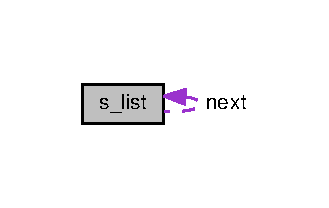
\includegraphics[width=158pt]{structs__list__coll__graph}
\end{center}
\end{figure}
\subsection*{Data Fields}
\begin{DoxyCompactItemize}
\item 
char $\ast$ {\bf file}
\item 
int {\bf double\-\_\-redi}
\item 
struct {\bf s\-\_\-list} $\ast$ {\bf next}
\end{DoxyCompactItemize}


\subsection{Detailed Description}


Definition at line 30 of file shell.\-h.



\subsection{Field Documentation}
\index{s\-\_\-list@{s\-\_\-list}!double\-\_\-redi@{double\-\_\-redi}}
\index{double\-\_\-redi@{double\-\_\-redi}!s_list@{s\-\_\-list}}
\subsubsection[{double\-\_\-redi}]{\setlength{\rightskip}{0pt plus 5cm}int double\-\_\-redi}\label{structs__list_a47fd463223ac923d306c984fb143dfa4}


Definition at line 33 of file shell.\-h.

\index{s\-\_\-list@{s\-\_\-list}!file@{file}}
\index{file@{file}!s_list@{s\-\_\-list}}
\subsubsection[{file}]{\setlength{\rightskip}{0pt plus 5cm}char$\ast$ file}\label{structs__list_adf16cd437526a5c5e0e0af87745acbb8}


Definition at line 32 of file shell.\-h.

\index{s\-\_\-list@{s\-\_\-list}!next@{next}}
\index{next@{next}!s_list@{s\-\_\-list}}
\subsubsection[{next}]{\setlength{\rightskip}{0pt plus 5cm}struct {\bf s\-\_\-list}$\ast$ next}\label{structs__list_a4bcaaa089cc834cf70b73bafa9af1e05}


Definition at line 34 of file shell.\-h.



The documentation for this struct was generated from the following file\-:\begin{DoxyCompactItemize}
\item 
include/{\bf shell.\-h}\end{DoxyCompactItemize}

\section{s\-\_\-list\-\_\-line Struct Reference}
\label{structs__list__line}\index{s\-\_\-list\-\_\-line@{s\-\_\-list\-\_\-line}}


{\ttfamily \#include $<$shell.\-h$>$}



Collaboration diagram for s\-\_\-list\-\_\-line\-:\nopagebreak
\begin{figure}[H]
\begin{center}
\leavevmode
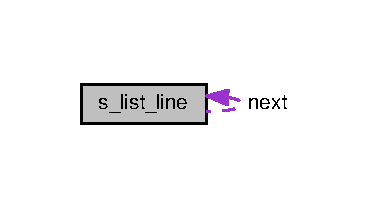
\includegraphics[width=179pt]{structs__list__line__coll__graph}
\end{center}
\end{figure}
\subsection*{Data Fields}
\begin{DoxyCompactItemize}
\item 
char $\ast$ {\bf line}
\item 
struct {\bf s\-\_\-list\-\_\-line} $\ast$ {\bf next}
\end{DoxyCompactItemize}


\subsection{Detailed Description}


Definition at line 24 of file shell.\-h.



\subsection{Field Documentation}
\index{s\-\_\-list\-\_\-line@{s\-\_\-list\-\_\-line}!line@{line}}
\index{line@{line}!s_list_line@{s\-\_\-list\-\_\-line}}
\subsubsection[{line}]{\setlength{\rightskip}{0pt plus 5cm}char$\ast$ line}\label{structs__list__line_a8adb30f4f6669f927fd9232f686c637b}


Definition at line 26 of file shell.\-h.

\index{s\-\_\-list\-\_\-line@{s\-\_\-list\-\_\-line}!next@{next}}
\index{next@{next}!s_list_line@{s\-\_\-list\-\_\-line}}
\subsubsection[{next}]{\setlength{\rightskip}{0pt plus 5cm}struct {\bf s\-\_\-list\-\_\-line}$\ast$ next}\label{structs__list__line_a3263d832fe4969fc3f9dbd0e668e0935}


Definition at line 27 of file shell.\-h.



The documentation for this struct was generated from the following file\-:\begin{DoxyCompactItemize}
\item 
include/{\bf shell.\-h}\end{DoxyCompactItemize}

\section{s\-\_\-stock Struct Reference}
\label{structs__stock}\index{s\-\_\-stock@{s\-\_\-stock}}


{\ttfamily \#include $<$shell.\-h$>$}

\subsection*{Data Fields}
\begin{DoxyCompactItemize}
\item 
char $\ast$ {\bf cmd}
\item 
char $\ast$ {\bf c}
\item 
int {\bf pos}
\end{DoxyCompactItemize}


\subsection{Detailed Description}


Definition at line 52 of file shell.\-h.



\subsection{Field Documentation}
\index{s\-\_\-stock@{s\-\_\-stock}!c@{c}}
\index{c@{c}!s_stock@{s\-\_\-stock}}
\subsubsection[{c}]{\setlength{\rightskip}{0pt plus 5cm}char$\ast$ c}\label{structs__stock_a9df78bd38aa81763ad1c56f3de8d5d3e}


Definition at line 55 of file shell.\-h.

\index{s\-\_\-stock@{s\-\_\-stock}!cmd@{cmd}}
\index{cmd@{cmd}!s_stock@{s\-\_\-stock}}
\subsubsection[{cmd}]{\setlength{\rightskip}{0pt plus 5cm}char$\ast$ cmd}\label{structs__stock_a7353cae57e2530c316ddacb27ef14932}


Definition at line 54 of file shell.\-h.

\index{s\-\_\-stock@{s\-\_\-stock}!pos@{pos}}
\index{pos@{pos}!s_stock@{s\-\_\-stock}}
\subsubsection[{pos}]{\setlength{\rightskip}{0pt plus 5cm}int pos}\label{structs__stock_a1910d262855b71da353ed0d07a6c7823}


Definition at line 56 of file shell.\-h.



The documentation for this struct was generated from the following file\-:\begin{DoxyCompactItemize}
\item 
include/{\bf shell.\-h}\end{DoxyCompactItemize}

\chapter{File Documentation}
\section{alias/alias.c File Reference}
\label{alias_8c}\index{alias/alias.\-c@{alias/alias.\-c}}
{\ttfamily \#include $<$stdlib.\-h$>$}\\*
{\ttfamily \#include $<$string.\-h$>$}\\*
{\ttfamily \#include $<$sys/types.\-h$>$}\\*
{\ttfamily \#include $<$sys/stat.\-h$>$}\\*
{\ttfamily \#include $<$fcntl.\-h$>$}\\*
{\ttfamily \#include $<$unistd.\-h$>$}\\*
{\ttfamily \#include $<$stdio.\-h$>$}\\*
{\ttfamily \#include \char`\"{}shell.\-h\char`\"{}}\\*
{\ttfamily \#include \char`\"{}lib.\-h\char`\"{}}\\*
Include dependency graph for alias.\-c\-:\nopagebreak
\begin{figure}[H]
\begin{center}
\leavevmode
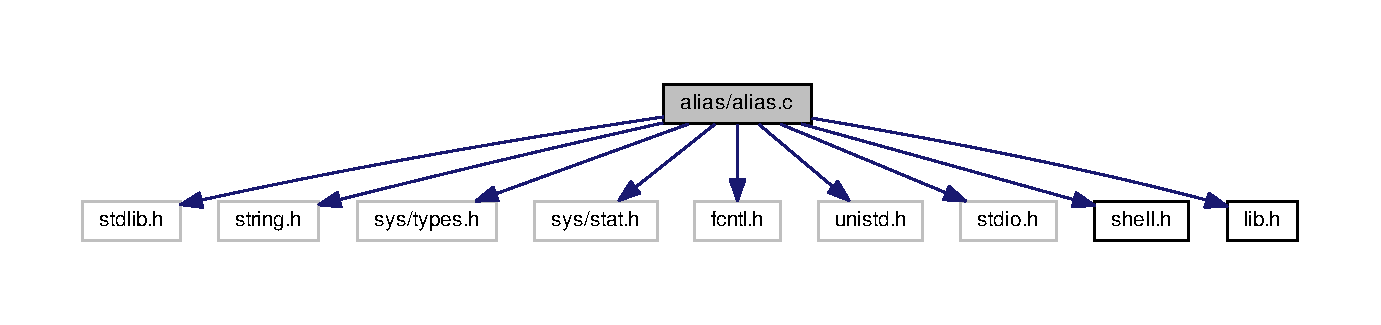
\includegraphics[width=350pt]{alias_8c__incl}
\end{center}
\end{figure}
\subsection*{Functions}
\begin{DoxyCompactItemize}
\item 
{\bf t\-\_\-alias} $\ast$ {\bf new\-\_\-alias} ({\bf t\-\_\-alias} $\ast$old, char $\ast$first, char $\ast$sec)
\item 
char $\ast$ {\bf alias\-\_\-finder} ({\bf t\-\_\-alias} $\ast$s, char $\ast$alias)
\item 
int {\bf get\-\_\-line\-\_\-file} ()
\item 
char $\ast$ {\bf alias\-\_\-find} ({\bf t\-\_\-alias} $\ast$alias, char $\ast$to\-\_\-find)
\item 
{\bf t\-\_\-data} $\ast$ {\bf check\-\_\-recur} ({\bf t\-\_\-data} $\ast$data, char $\ast$old, char $\ast$new)
\end{DoxyCompactItemize}


\subsection{Function Documentation}
\index{alias.\-c@{alias.\-c}!alias\-\_\-find@{alias\-\_\-find}}
\index{alias\-\_\-find@{alias\-\_\-find}!alias.c@{alias.\-c}}
\subsubsection[{alias\-\_\-find}]{\setlength{\rightskip}{0pt plus 5cm}char$\ast$ alias\-\_\-find (
\begin{DoxyParamCaption}
\item[{{\bf t\-\_\-alias} $\ast$}]{alias, }
\item[{char $\ast$}]{to\-\_\-find}
\end{DoxyParamCaption}
)}\label{alias_8c_ac8db3662f7b7cc7ee5b03b6c5591447d}


Definition at line 74 of file alias.\-c.



Here is the call graph for this function\-:
\nopagebreak
\begin{figure}[H]
\begin{center}
\leavevmode
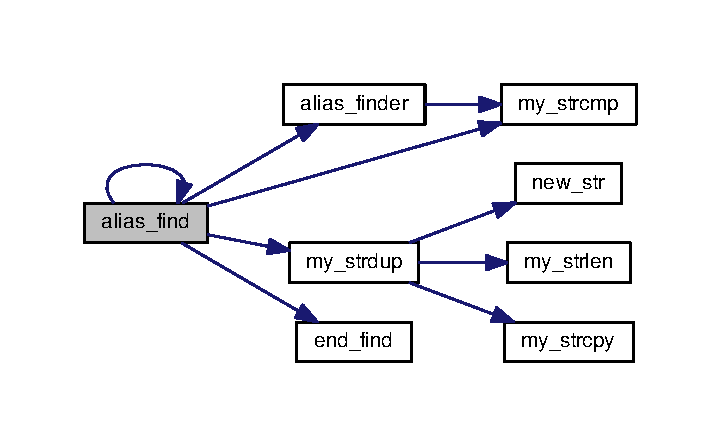
\includegraphics[width=346pt]{alias_8c_ac8db3662f7b7cc7ee5b03b6c5591447d_cgraph}
\end{center}
\end{figure}




Here is the caller graph for this function\-:\nopagebreak
\begin{figure}[H]
\begin{center}
\leavevmode
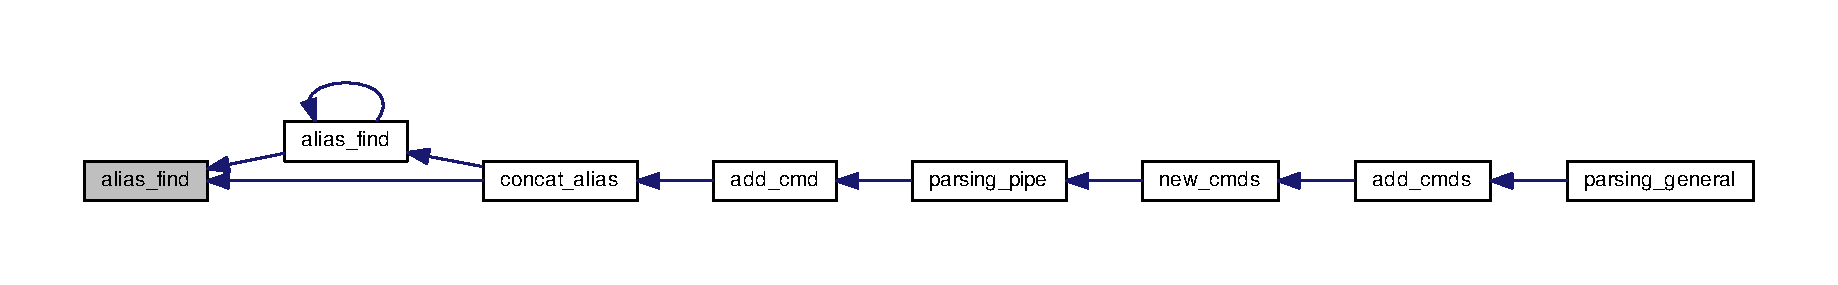
\includegraphics[width=350pt]{alias_8c_ac8db3662f7b7cc7ee5b03b6c5591447d_icgraph}
\end{center}
\end{figure}


\index{alias.\-c@{alias.\-c}!alias\-\_\-finder@{alias\-\_\-finder}}
\index{alias\-\_\-finder@{alias\-\_\-finder}!alias.c@{alias.\-c}}
\subsubsection[{alias\-\_\-finder}]{\setlength{\rightskip}{0pt plus 5cm}char$\ast$ alias\-\_\-finder (
\begin{DoxyParamCaption}
\item[{{\bf t\-\_\-alias} $\ast$}]{s, }
\item[{char $\ast$}]{alias}
\end{DoxyParamCaption}
)}\label{alias_8c_ae7ca988050564368cd481dd94902435b}


Definition at line 40 of file alias.\-c.



Here is the call graph for this function\-:\nopagebreak
\begin{figure}[H]
\begin{center}
\leavevmode
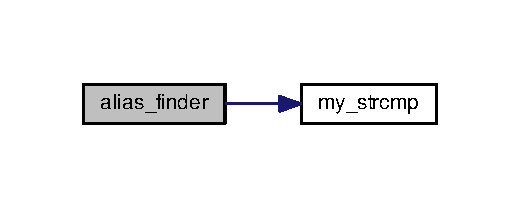
\includegraphics[width=250pt]{alias_8c_ae7ca988050564368cd481dd94902435b_cgraph}
\end{center}
\end{figure}




Here is the caller graph for this function\-:\nopagebreak
\begin{figure}[H]
\begin{center}
\leavevmode
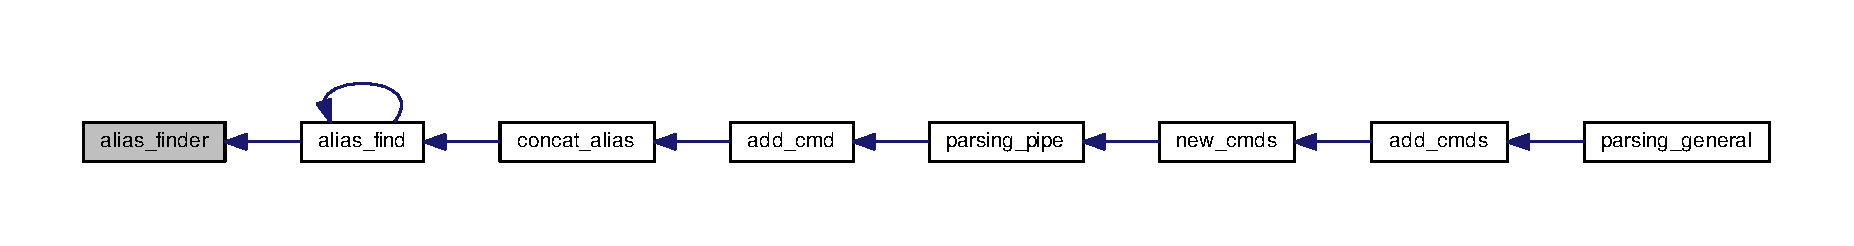
\includegraphics[width=350pt]{alias_8c_ae7ca988050564368cd481dd94902435b_icgraph}
\end{center}
\end{figure}


\index{alias.\-c@{alias.\-c}!check\-\_\-recur@{check\-\_\-recur}}
\index{check\-\_\-recur@{check\-\_\-recur}!alias.c@{alias.\-c}}
\subsubsection[{check\-\_\-recur}]{\setlength{\rightskip}{0pt plus 5cm}{\bf t\-\_\-data}$\ast$ check\-\_\-recur (
\begin{DoxyParamCaption}
\item[{{\bf t\-\_\-data} $\ast$}]{data, }
\item[{char $\ast$}]{old, }
\item[{char $\ast$}]{new}
\end{DoxyParamCaption}
)}\label{alias_8c_afa6fff44bde50c8a0f4b8868f6b81777}


Definition at line 102 of file alias.\-c.



Here is the call graph for this function\-:\nopagebreak
\begin{figure}[H]
\begin{center}
\leavevmode
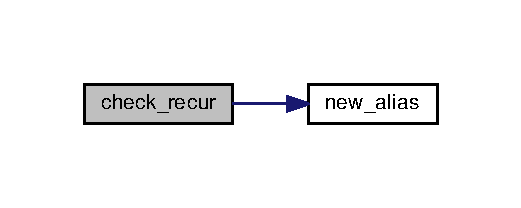
\includegraphics[width=250pt]{alias_8c_afa6fff44bde50c8a0f4b8868f6b81777_cgraph}
\end{center}
\end{figure}




Here is the caller graph for this function\-:\nopagebreak
\begin{figure}[H]
\begin{center}
\leavevmode
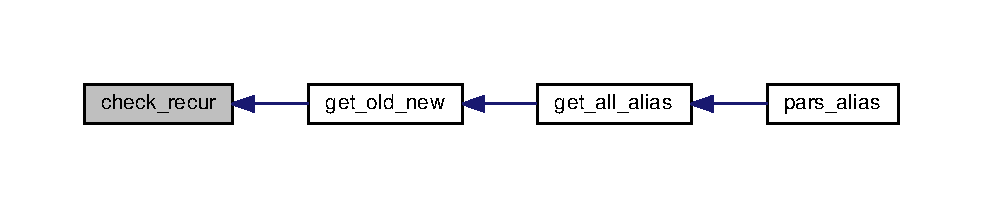
\includegraphics[width=350pt]{alias_8c_afa6fff44bde50c8a0f4b8868f6b81777_icgraph}
\end{center}
\end{figure}


\index{alias.\-c@{alias.\-c}!get\-\_\-line\-\_\-file@{get\-\_\-line\-\_\-file}}
\index{get\-\_\-line\-\_\-file@{get\-\_\-line\-\_\-file}!alias.c@{alias.\-c}}
\subsubsection[{get\-\_\-line\-\_\-file}]{\setlength{\rightskip}{0pt plus 5cm}int get\-\_\-line\-\_\-file (
\begin{DoxyParamCaption}
{}
\end{DoxyParamCaption}
)}\label{alias_8c_adea8df0d450d18361023ed783f462f39}


Definition at line 56 of file alias.\-c.



Here is the call graph for this function\-:\nopagebreak
\begin{figure}[H]
\begin{center}
\leavevmode
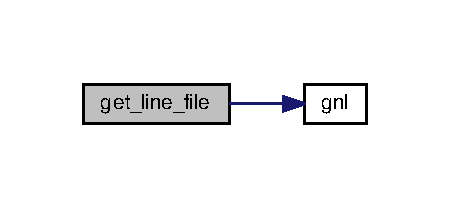
\includegraphics[width=216pt]{alias_8c_adea8df0d450d18361023ed783f462f39_cgraph}
\end{center}
\end{figure}




Here is the caller graph for this function\-:\nopagebreak
\begin{figure}[H]
\begin{center}
\leavevmode
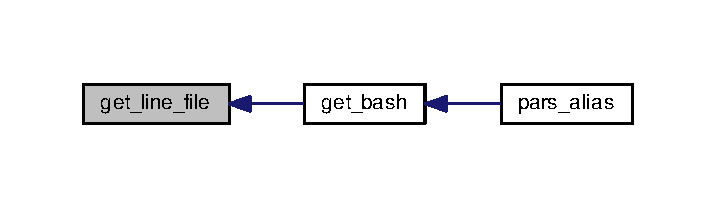
\includegraphics[width=344pt]{alias_8c_adea8df0d450d18361023ed783f462f39_icgraph}
\end{center}
\end{figure}


\index{alias.\-c@{alias.\-c}!new\-\_\-alias@{new\-\_\-alias}}
\index{new\-\_\-alias@{new\-\_\-alias}!alias.c@{alias.\-c}}
\subsubsection[{new\-\_\-alias}]{\setlength{\rightskip}{0pt plus 5cm}{\bf t\-\_\-alias}$\ast$ new\-\_\-alias (
\begin{DoxyParamCaption}
\item[{{\bf t\-\_\-alias} $\ast$}]{old, }
\item[{char $\ast$}]{first, }
\item[{char $\ast$}]{sec}
\end{DoxyParamCaption}
)}\label{alias_8c_ad5f519b4cbb35030e5d5713a466439e7}


Definition at line 21 of file alias.\-c.



Here is the caller graph for this function\-:\nopagebreak
\begin{figure}[H]
\begin{center}
\leavevmode
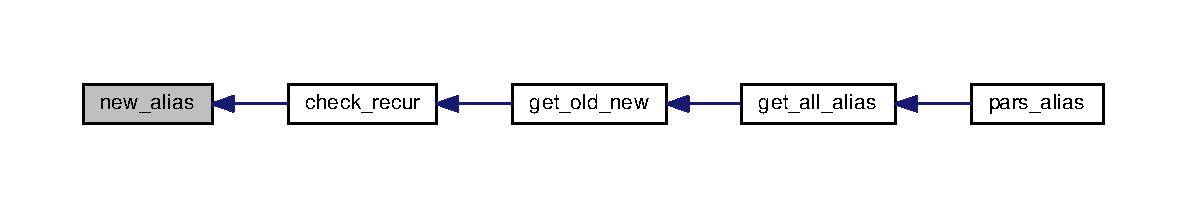
\includegraphics[width=350pt]{alias_8c_ad5f519b4cbb35030e5d5713a466439e7_icgraph}
\end{center}
\end{figure}



\section{alias/alias\-\_\-etc.c File Reference}
\label{alias__etc_8c}\index{alias/alias\-\_\-etc.\-c@{alias/alias\-\_\-etc.\-c}}
{\ttfamily \#include $<$stdlib.\-h$>$}\\*
{\ttfamily \#include \char`\"{}lib.\-h\char`\"{}}\\*
{\ttfamily \#include \char`\"{}shell.\-h\char`\"{}}\\*
{\ttfamily \#include \char`\"{}builtin.\-h\char`\"{}}\\*
Include dependency graph for alias\-\_\-etc.\-c\-:
\nopagebreak
\begin{figure}[H]
\begin{center}
\leavevmode
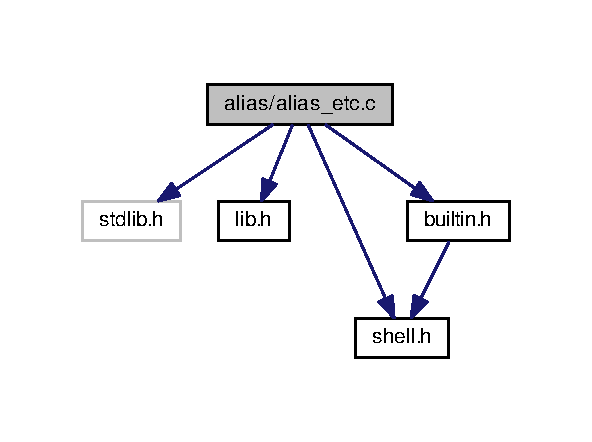
\includegraphics[width=284pt]{alias__etc_8c__incl}
\end{center}
\end{figure}
\subsection*{Functions}
\begin{DoxyCompactItemize}
\item 
int {\bf setbashenv} (int i, char $\ast$str, int start, char $\ast$$\ast$to\-\_\-set)
\item 
int {\bf bashset} (char $\ast$str, {\bf t\-\_\-data} $\ast$data)
\item 
char $\ast$ {\bf end\-\_\-find} (char $\ast$new, char $\ast$prev, char $\ast$to\-\_\-find)
\item 
char $\ast$ {\bf concat\-\_\-alias} (char $\ast$str, {\bf t\-\_\-alias} $\ast$list\-\_\-alias)
\end{DoxyCompactItemize}


\subsection{Function Documentation}
\index{alias\-\_\-etc.\-c@{alias\-\_\-etc.\-c}!bashset@{bashset}}
\index{bashset@{bashset}!alias_etc.c@{alias\-\_\-etc.\-c}}
\subsubsection[{bashset}]{\setlength{\rightskip}{0pt plus 5cm}int bashset (
\begin{DoxyParamCaption}
\item[{char $\ast$}]{str, }
\item[{{\bf t\-\_\-data} $\ast$}]{data}
\end{DoxyParamCaption}
)}\label{alias__etc_8c_acd9ad0dfae53c8683ec2597a188e6c1b}


Definition at line 33 of file alias\-\_\-etc.\-c.



Here is the call graph for this function\-:\nopagebreak
\begin{figure}[H]
\begin{center}
\leavevmode
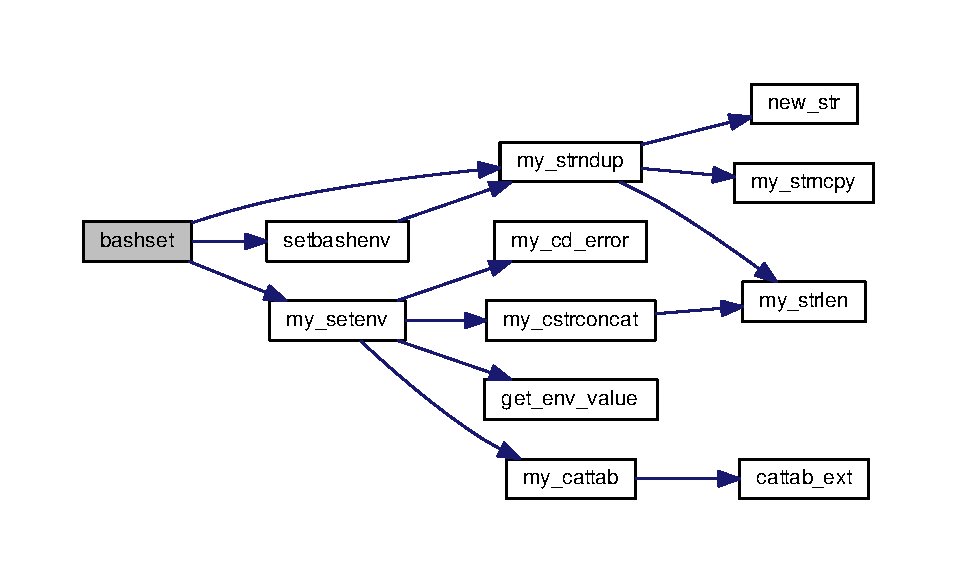
\includegraphics[width=350pt]{alias__etc_8c_acd9ad0dfae53c8683ec2597a188e6c1b_cgraph}
\end{center}
\end{figure}




Here is the caller graph for this function\-:\nopagebreak
\begin{figure}[H]
\begin{center}
\leavevmode
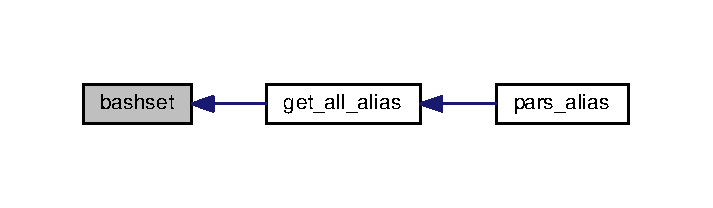
\includegraphics[width=342pt]{alias__etc_8c_acd9ad0dfae53c8683ec2597a188e6c1b_icgraph}
\end{center}
\end{figure}


\index{alias\-\_\-etc.\-c@{alias\-\_\-etc.\-c}!concat\-\_\-alias@{concat\-\_\-alias}}
\index{concat\-\_\-alias@{concat\-\_\-alias}!alias_etc.c@{alias\-\_\-etc.\-c}}
\subsubsection[{concat\-\_\-alias}]{\setlength{\rightskip}{0pt plus 5cm}char$\ast$ concat\-\_\-alias (
\begin{DoxyParamCaption}
\item[{char $\ast$}]{str, }
\item[{{\bf t\-\_\-alias} $\ast$}]{list\-\_\-alias}
\end{DoxyParamCaption}
)}\label{alias__etc_8c_a2cede4e33e1a1250deaee16f518024c4}


Definition at line 71 of file alias\-\_\-etc.\-c.



Here is the call graph for this function\-:
\nopagebreak
\begin{figure}[H]
\begin{center}
\leavevmode
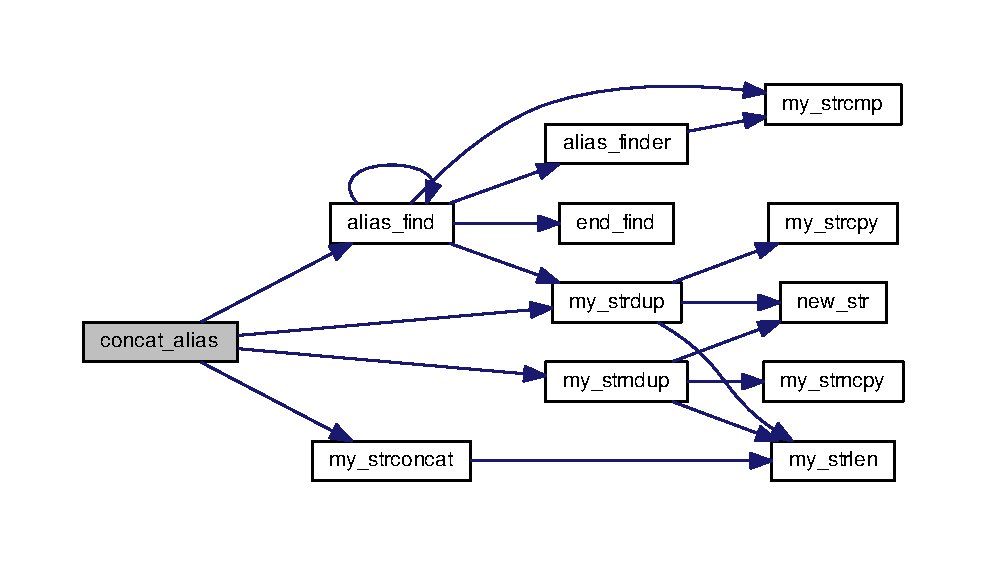
\includegraphics[width=350pt]{alias__etc_8c_a2cede4e33e1a1250deaee16f518024c4_cgraph}
\end{center}
\end{figure}




Here is the caller graph for this function\-:\nopagebreak
\begin{figure}[H]
\begin{center}
\leavevmode
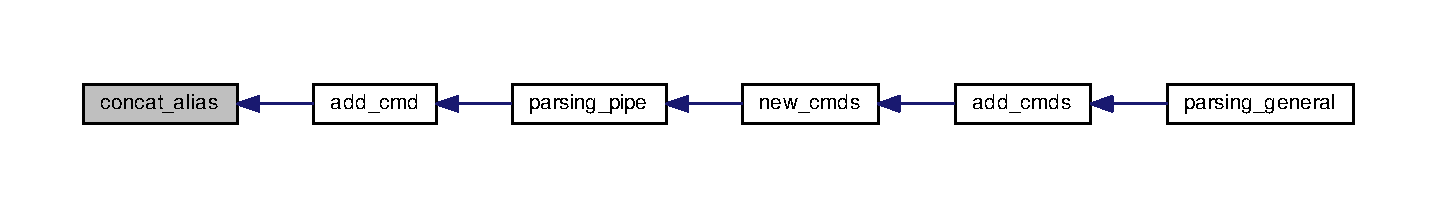
\includegraphics[width=350pt]{alias__etc_8c_a2cede4e33e1a1250deaee16f518024c4_icgraph}
\end{center}
\end{figure}


\index{alias\-\_\-etc.\-c@{alias\-\_\-etc.\-c}!end\-\_\-find@{end\-\_\-find}}
\index{end\-\_\-find@{end\-\_\-find}!alias_etc.c@{alias\-\_\-etc.\-c}}
\subsubsection[{end\-\_\-find}]{\setlength{\rightskip}{0pt plus 5cm}char$\ast$ end\-\_\-find (
\begin{DoxyParamCaption}
\item[{char $\ast$}]{new, }
\item[{char $\ast$}]{prev, }
\item[{char $\ast$}]{to\-\_\-find}
\end{DoxyParamCaption}
)}\label{alias__etc_8c_aeee2c96c8e8193fc245dee41ac044a77}


Definition at line 62 of file alias\-\_\-etc.\-c.



Here is the caller graph for this function\-:
\nopagebreak
\begin{figure}[H]
\begin{center}
\leavevmode
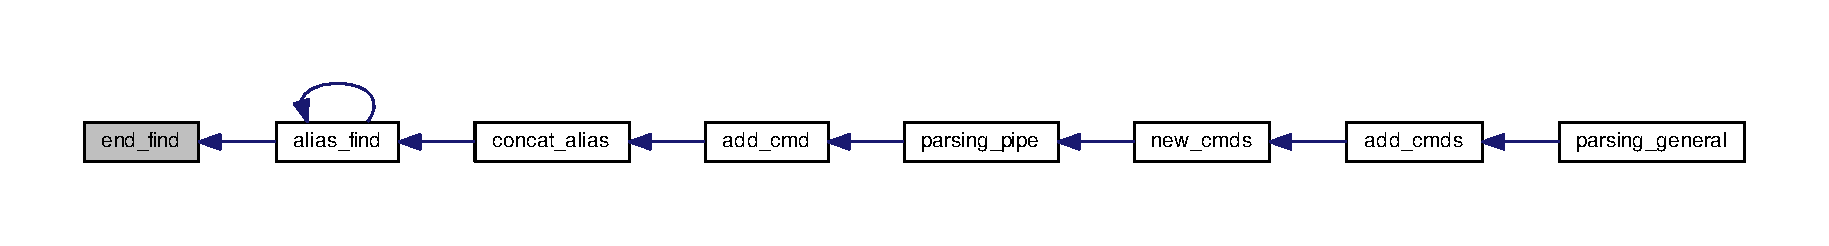
\includegraphics[width=350pt]{alias__etc_8c_aeee2c96c8e8193fc245dee41ac044a77_icgraph}
\end{center}
\end{figure}


\index{alias\-\_\-etc.\-c@{alias\-\_\-etc.\-c}!setbashenv@{setbashenv}}
\index{setbashenv@{setbashenv}!alias_etc.c@{alias\-\_\-etc.\-c}}
\subsubsection[{setbashenv}]{\setlength{\rightskip}{0pt plus 5cm}int setbashenv (
\begin{DoxyParamCaption}
\item[{int}]{i, }
\item[{char $\ast$}]{str, }
\item[{int}]{start, }
\item[{char $\ast$$\ast$}]{to\-\_\-set}
\end{DoxyParamCaption}
)}\label{alias__etc_8c_a2554b2fd4cf3639ec091ec6a5a432675}


Definition at line 20 of file alias\-\_\-etc.\-c.



Here is the call graph for this function\-:\nopagebreak
\begin{figure}[H]
\begin{center}
\leavevmode
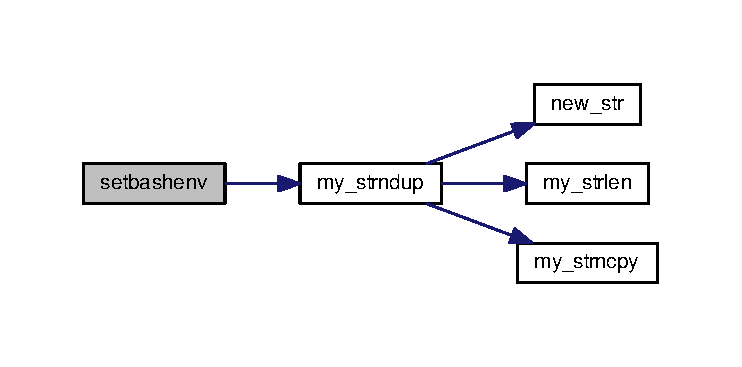
\includegraphics[width=350pt]{alias__etc_8c_a2554b2fd4cf3639ec091ec6a5a432675_cgraph}
\end{center}
\end{figure}




Here is the caller graph for this function\-:\nopagebreak
\begin{figure}[H]
\begin{center}
\leavevmode
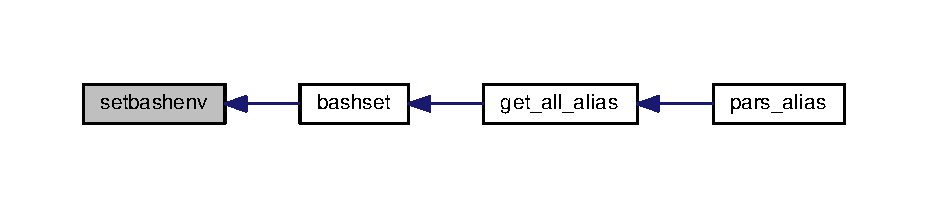
\includegraphics[width=350pt]{alias__etc_8c_a2554b2fd4cf3639ec091ec6a5a432675_icgraph}
\end{center}
\end{figure}



\section{alias/gnl.c File Reference}
\label{gnl_8c}\index{alias/gnl.\-c@{alias/gnl.\-c}}
{\ttfamily \#include $<$stdlib.\-h$>$}\\*
{\ttfamily \#include $<$string.\-h$>$}\\*
{\ttfamily \#include $<$sys/types.\-h$>$}\\*
{\ttfamily \#include $<$sys/stat.\-h$>$}\\*
{\ttfamily \#include $<$fcntl.\-h$>$}\\*
{\ttfamily \#include $<$unistd.\-h$>$}\\*
{\ttfamily \#include \char`\"{}shell.\-h\char`\"{}}\\*
Include dependency graph for gnl.\-c\-:\nopagebreak
\begin{figure}[H]
\begin{center}
\leavevmode
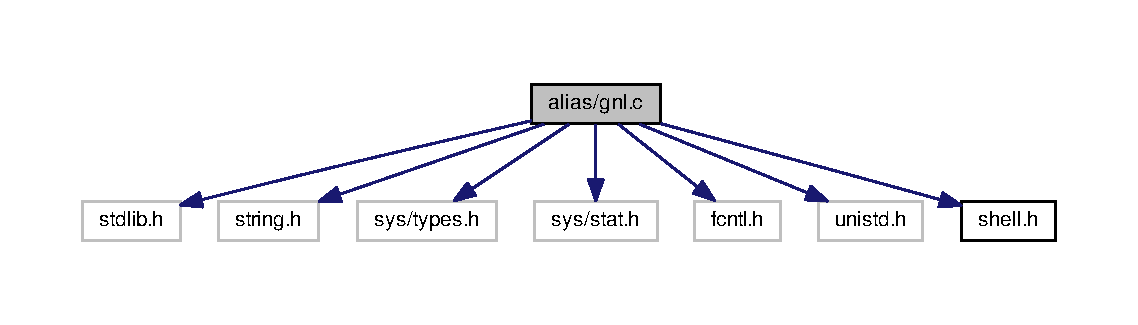
\includegraphics[width=350pt]{gnl_8c__incl}
\end{center}
\end{figure}
\subsection*{Functions}
\begin{DoxyCompactItemize}
\item 
char $\ast$ {\bf gnl} (const int fd)
\end{DoxyCompactItemize}


\subsection{Function Documentation}
\index{gnl.\-c@{gnl.\-c}!gnl@{gnl}}
\index{gnl@{gnl}!gnl.c@{gnl.\-c}}
\subsubsection[{gnl}]{\setlength{\rightskip}{0pt plus 5cm}char$\ast$ gnl (
\begin{DoxyParamCaption}
\item[{const int}]{fd}
\end{DoxyParamCaption}
)}\label{gnl_8c_a6754f4915186decc3a861cd78d15499e}


Definition at line 73 of file gnl.\-c.



Here is the caller graph for this function\-:\nopagebreak
\begin{figure}[H]
\begin{center}
\leavevmode
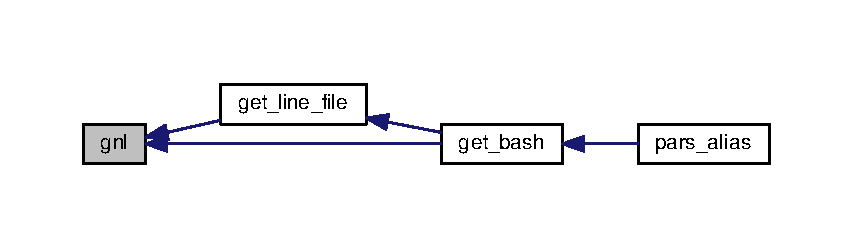
\includegraphics[width=350pt]{gnl_8c_a6754f4915186decc3a861cd78d15499e_icgraph}
\end{center}
\end{figure}



\section{alias/pars\-\_\-alias.c File Reference}
\label{pars__alias_8c}\index{alias/pars\-\_\-alias.\-c@{alias/pars\-\_\-alias.\-c}}
{\ttfamily \#include $<$stdlib.\-h$>$}\\*
{\ttfamily \#include $<$sys/types.\-h$>$}\\*
{\ttfamily \#include $<$sys/stat.\-h$>$}\\*
{\ttfamily \#include $<$fcntl.\-h$>$}\\*
{\ttfamily \#include $<$unistd.\-h$>$}\\*
{\ttfamily \#include $<$stdio.\-h$>$}\\*
{\ttfamily \#include \char`\"{}builtin.\-h\char`\"{}}\\*
{\ttfamily \#include \char`\"{}shell.\-h\char`\"{}}\\*
{\ttfamily \#include \char`\"{}lib.\-h\char`\"{}}\\*
Include dependency graph for pars\-\_\-alias.\-c\-:
\nopagebreak
\begin{figure}[H]
\begin{center}
\leavevmode
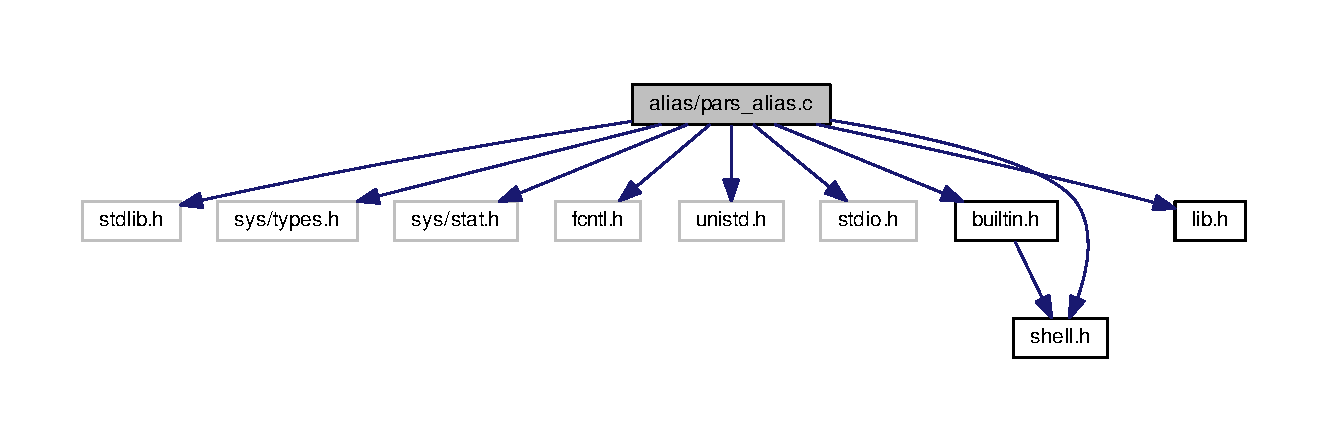
\includegraphics[width=350pt]{pars__alias_8c__incl}
\end{center}
\end{figure}
\subsection*{Functions}
\begin{DoxyCompactItemize}
\item 
char $\ast$$\ast$ {\bf get\-\_\-bash} ()
\item 
char $\ast$ {\bf get\-\_\-old} (char $\ast$str, int x, int i)
\item 
{\bf t\-\_\-data} $\ast$ {\bf get\-\_\-old\-\_\-new} (char $\ast$str, {\bf t\-\_\-data} $\ast$data, int x)
\item 
{\bf t\-\_\-data} $\ast$ {\bf get\-\_\-all\-\_\-alias} ({\bf t\-\_\-data} $\ast$data, char $\ast$$\ast$bash, int x)
\item 
int {\bf pars\-\_\-alias} ({\bf t\-\_\-data} $\ast$data)
\end{DoxyCompactItemize}


\subsection{Function Documentation}
\index{pars\-\_\-alias.\-c@{pars\-\_\-alias.\-c}!get\-\_\-all\-\_\-alias@{get\-\_\-all\-\_\-alias}}
\index{get\-\_\-all\-\_\-alias@{get\-\_\-all\-\_\-alias}!pars_alias.c@{pars\-\_\-alias.\-c}}
\subsubsection[{get\-\_\-all\-\_\-alias}]{\setlength{\rightskip}{0pt plus 5cm}{\bf t\-\_\-data}$\ast$ get\-\_\-all\-\_\-alias (
\begin{DoxyParamCaption}
\item[{{\bf t\-\_\-data} $\ast$}]{data, }
\item[{char $\ast$$\ast$}]{bash, }
\item[{int}]{x}
\end{DoxyParamCaption}
)}\label{pars__alias_8c_a94ed7403f0bc582353a563669932efdd}


Definition at line 100 of file pars\-\_\-alias.\-c.



Here is the call graph for this function\-:\nopagebreak
\begin{figure}[H]
\begin{center}
\leavevmode
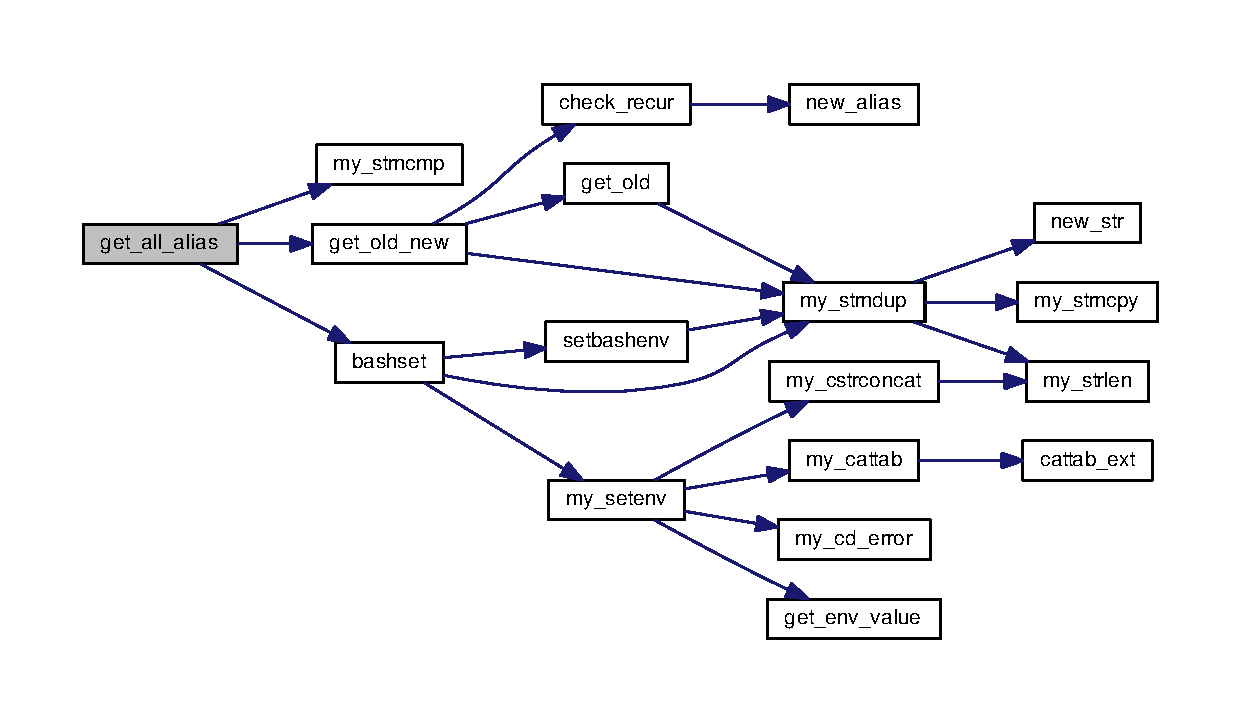
\includegraphics[width=350pt]{pars__alias_8c_a94ed7403f0bc582353a563669932efdd_cgraph}
\end{center}
\end{figure}




Here is the caller graph for this function\-:\nopagebreak
\begin{figure}[H]
\begin{center}
\leavevmode
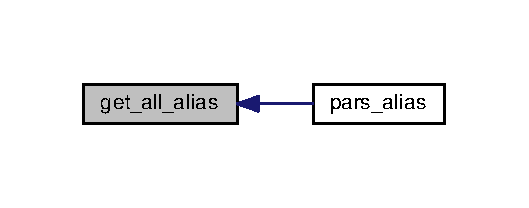
\includegraphics[width=254pt]{pars__alias_8c_a94ed7403f0bc582353a563669932efdd_icgraph}
\end{center}
\end{figure}


\index{pars\-\_\-alias.\-c@{pars\-\_\-alias.\-c}!get\-\_\-bash@{get\-\_\-bash}}
\index{get\-\_\-bash@{get\-\_\-bash}!pars_alias.c@{pars\-\_\-alias.\-c}}
\subsubsection[{get\-\_\-bash}]{\setlength{\rightskip}{0pt plus 5cm}char$\ast$$\ast$ get\-\_\-bash (
\begin{DoxyParamCaption}
{}
\end{DoxyParamCaption}
)}\label{pars__alias_8c_a203bc66f586da530ebb9eeee519bd082}


Definition at line 21 of file pars\-\_\-alias.\-c.



Here is the call graph for this function\-:\nopagebreak
\begin{figure}[H]
\begin{center}
\leavevmode
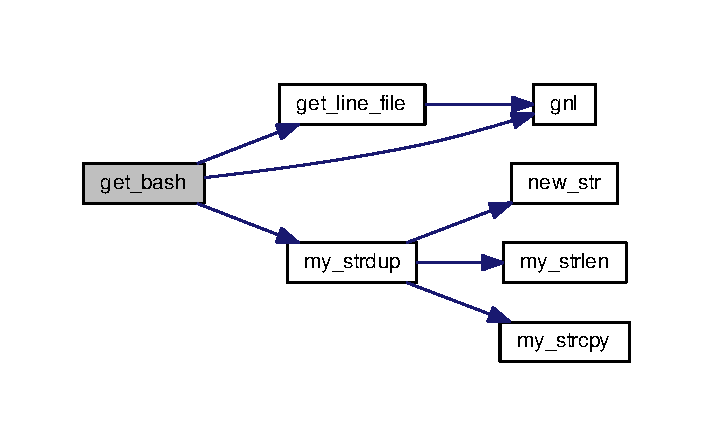
\includegraphics[width=342pt]{pars__alias_8c_a203bc66f586da530ebb9eeee519bd082_cgraph}
\end{center}
\end{figure}




Here is the caller graph for this function\-:\nopagebreak
\begin{figure}[H]
\begin{center}
\leavevmode
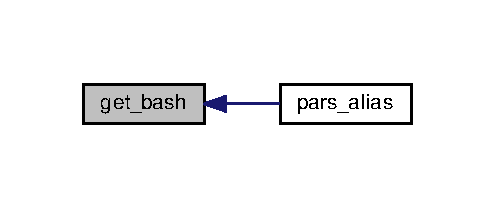
\includegraphics[width=238pt]{pars__alias_8c_a203bc66f586da530ebb9eeee519bd082_icgraph}
\end{center}
\end{figure}


\index{pars\-\_\-alias.\-c@{pars\-\_\-alias.\-c}!get\-\_\-old@{get\-\_\-old}}
\index{get\-\_\-old@{get\-\_\-old}!pars_alias.c@{pars\-\_\-alias.\-c}}
\subsubsection[{get\-\_\-old}]{\setlength{\rightskip}{0pt plus 5cm}char$\ast$ get\-\_\-old (
\begin{DoxyParamCaption}
\item[{char $\ast$}]{str, }
\item[{int}]{x, }
\item[{int}]{i}
\end{DoxyParamCaption}
)}\label{pars__alias_8c_a3257a6fcadd0309f1df178525eea9257}


Definition at line 47 of file pars\-\_\-alias.\-c.



Here is the call graph for this function\-:\nopagebreak
\begin{figure}[H]
\begin{center}
\leavevmode
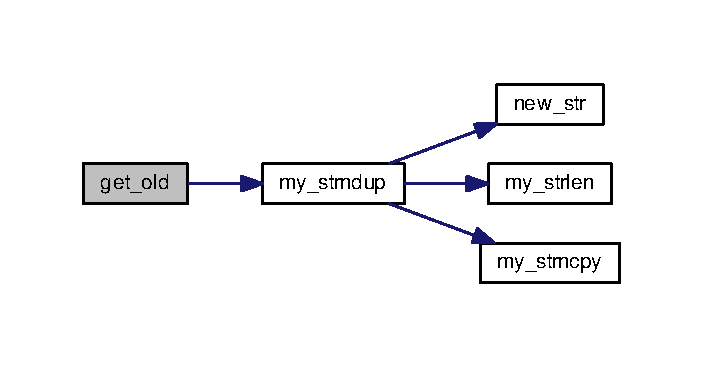
\includegraphics[width=338pt]{pars__alias_8c_a3257a6fcadd0309f1df178525eea9257_cgraph}
\end{center}
\end{figure}




Here is the caller graph for this function\-:\nopagebreak
\begin{figure}[H]
\begin{center}
\leavevmode
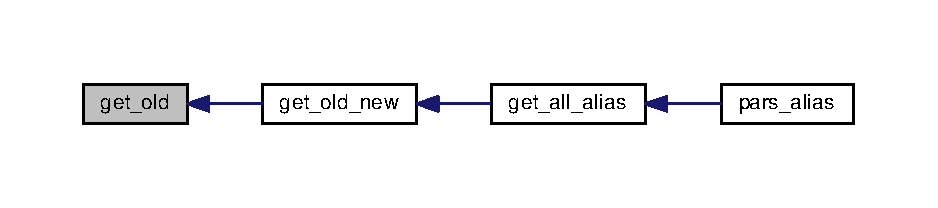
\includegraphics[width=350pt]{pars__alias_8c_a3257a6fcadd0309f1df178525eea9257_icgraph}
\end{center}
\end{figure}


\index{pars\-\_\-alias.\-c@{pars\-\_\-alias.\-c}!get\-\_\-old\-\_\-new@{get\-\_\-old\-\_\-new}}
\index{get\-\_\-old\-\_\-new@{get\-\_\-old\-\_\-new}!pars_alias.c@{pars\-\_\-alias.\-c}}
\subsubsection[{get\-\_\-old\-\_\-new}]{\setlength{\rightskip}{0pt plus 5cm}{\bf t\-\_\-data}$\ast$ get\-\_\-old\-\_\-new (
\begin{DoxyParamCaption}
\item[{char $\ast$}]{str, }
\item[{{\bf t\-\_\-data} $\ast$}]{data, }
\item[{int}]{x}
\end{DoxyParamCaption}
)}\label{pars__alias_8c_a7d7873e60a328ecd3a34c3370594b040}


Definition at line 76 of file pars\-\_\-alias.\-c.



Here is the call graph for this function\-:\nopagebreak
\begin{figure}[H]
\begin{center}
\leavevmode
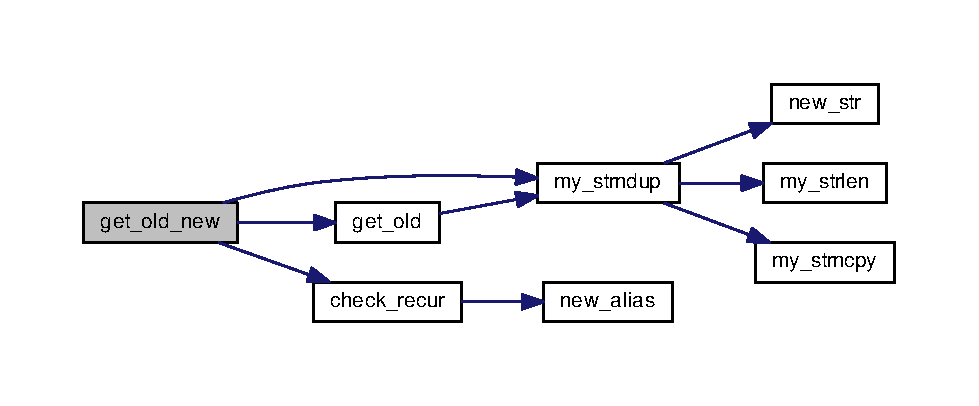
\includegraphics[width=350pt]{pars__alias_8c_a7d7873e60a328ecd3a34c3370594b040_cgraph}
\end{center}
\end{figure}




Here is the caller graph for this function\-:\nopagebreak
\begin{figure}[H]
\begin{center}
\leavevmode
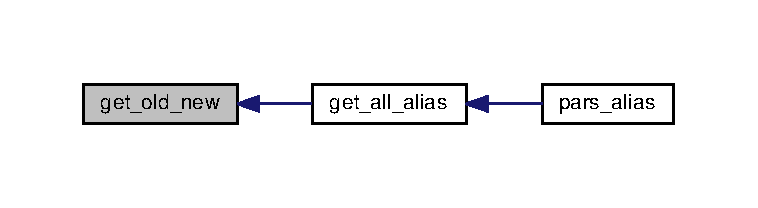
\includegraphics[width=350pt]{pars__alias_8c_a7d7873e60a328ecd3a34c3370594b040_icgraph}
\end{center}
\end{figure}


\index{pars\-\_\-alias.\-c@{pars\-\_\-alias.\-c}!pars\-\_\-alias@{pars\-\_\-alias}}
\index{pars\-\_\-alias@{pars\-\_\-alias}!pars_alias.c@{pars\-\_\-alias.\-c}}
\subsubsection[{pars\-\_\-alias}]{\setlength{\rightskip}{0pt plus 5cm}int pars\-\_\-alias (
\begin{DoxyParamCaption}
\item[{{\bf t\-\_\-data} $\ast$}]{data}
\end{DoxyParamCaption}
)}\label{pars__alias_8c_a8e5633ce3ca1c968f88de68f3ed735c7}


Definition at line 119 of file pars\-\_\-alias.\-c.



Here is the call graph for this function\-:\nopagebreak
\begin{figure}[H]
\begin{center}
\leavevmode
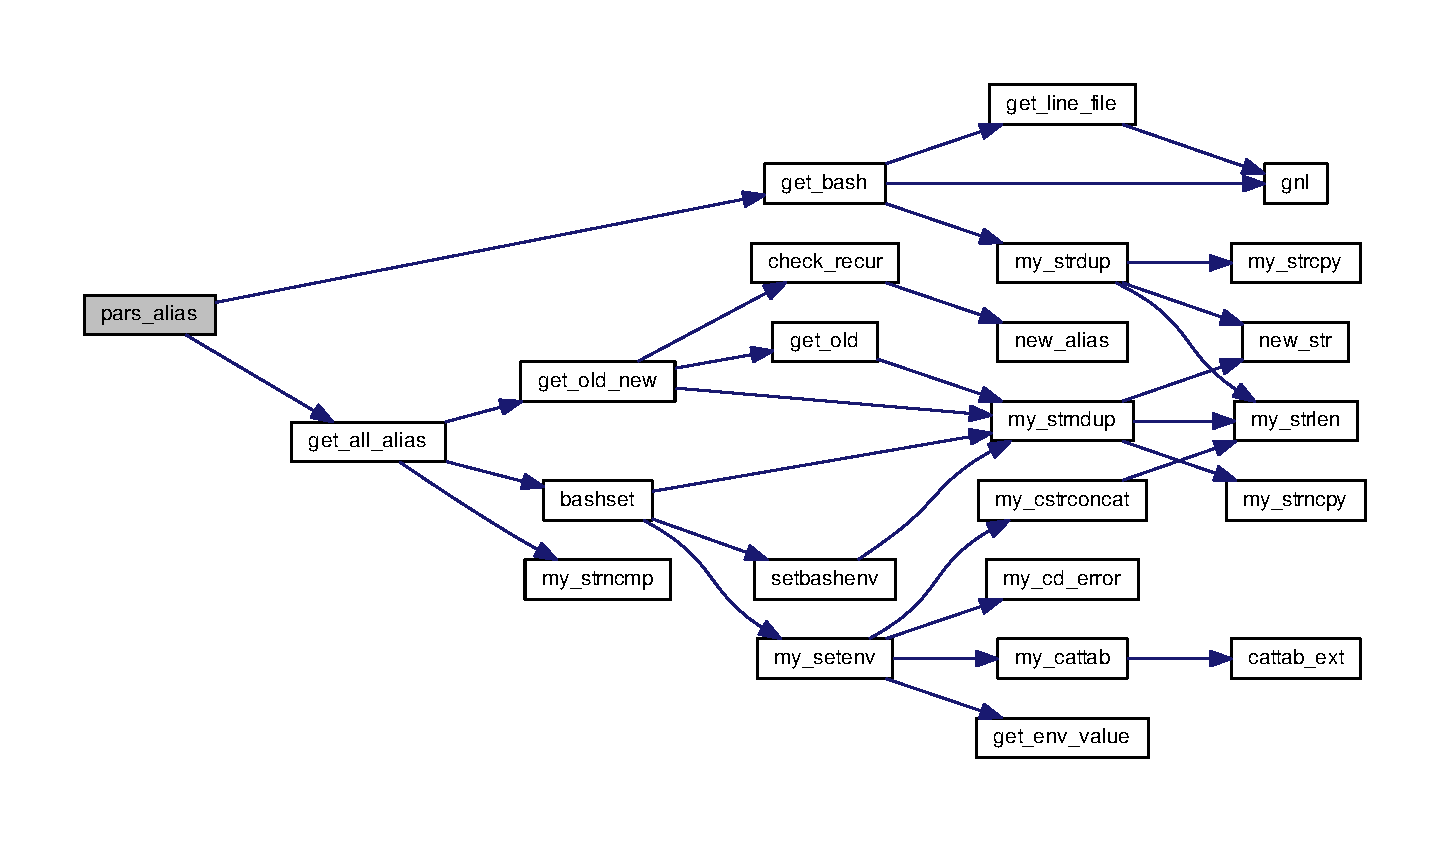
\includegraphics[width=350pt]{pars__alias_8c_a8e5633ce3ca1c968f88de68f3ed735c7_cgraph}
\end{center}
\end{figure}



\section{alias/str\-\_\-cat.c File Reference}
\label{str__cat_8c}\index{alias/str\-\_\-cat.\-c@{alias/str\-\_\-cat.\-c}}
{\ttfamily \#include $<$stdlib.\-h$>$}\\*
{\ttfamily \#include \char`\"{}lib.\-h\char`\"{}}\\*
Include dependency graph for str\-\_\-cat.\-c\-:\nopagebreak
\begin{figure}[H]
\begin{center}
\leavevmode
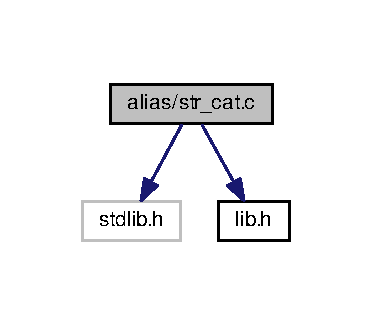
\includegraphics[width=179pt]{str__cat_8c__incl}
\end{center}
\end{figure}
\subsection*{Functions}
\begin{DoxyCompactItemize}
\item 
char $\ast$ {\bf my\-\_\-strconcat} (char $\ast$s1, char $\ast$s2)
\end{DoxyCompactItemize}


\subsection{Function Documentation}
\index{str\-\_\-cat.\-c@{str\-\_\-cat.\-c}!my\-\_\-strconcat@{my\-\_\-strconcat}}
\index{my\-\_\-strconcat@{my\-\_\-strconcat}!str_cat.c@{str\-\_\-cat.\-c}}
\subsubsection[{my\-\_\-strconcat}]{\setlength{\rightskip}{0pt plus 5cm}char$\ast$ my\-\_\-strconcat (
\begin{DoxyParamCaption}
\item[{char $\ast$}]{s1, }
\item[{char $\ast$}]{s2}
\end{DoxyParamCaption}
)}\label{str__cat_8c_ae2589b5e18e85e7f44abd6bddf4724a4}


Definition at line 14 of file str\-\_\-cat.\-c.



Here is the call graph for this function\-:\nopagebreak
\begin{figure}[H]
\begin{center}
\leavevmode
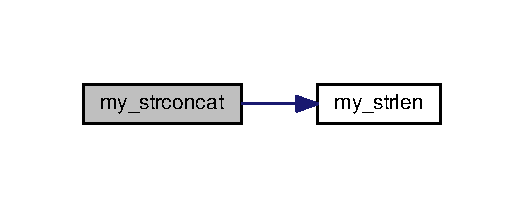
\includegraphics[width=252pt]{str__cat_8c_ae2589b5e18e85e7f44abd6bddf4724a4_cgraph}
\end{center}
\end{figure}




Here is the caller graph for this function\-:\nopagebreak
\begin{figure}[H]
\begin{center}
\leavevmode
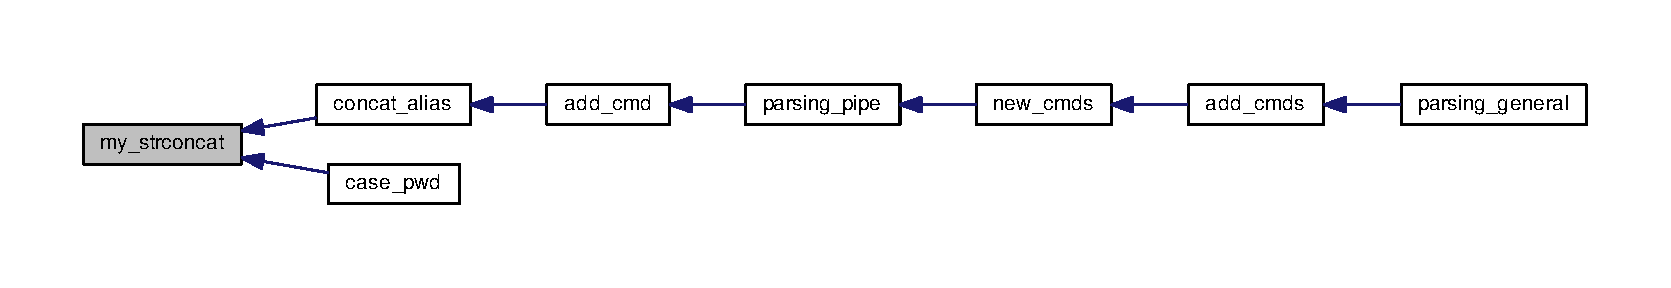
\includegraphics[width=350pt]{str__cat_8c_ae2589b5e18e85e7f44abd6bddf4724a4_icgraph}
\end{center}
\end{figure}



\section{auto\-\_\-complete/auto\-\_\-complete.c File Reference}
\label{auto__complete_8c}\index{auto\-\_\-complete/auto\-\_\-complete.\-c@{auto\-\_\-complete/auto\-\_\-complete.\-c}}
{\ttfamily \#include $<$stdlib.\-h$>$}\\*
{\ttfamily \#include $<$glob.\-h$>$}\\*
{\ttfamily \#include \char`\"{}lib.\-h\char`\"{}}\\*
{\ttfamily \#include \char`\"{}shell.\-h\char`\"{}}\\*
Include dependency graph for auto\-\_\-complete.\-c\-:\nopagebreak
\begin{figure}[H]
\begin{center}
\leavevmode
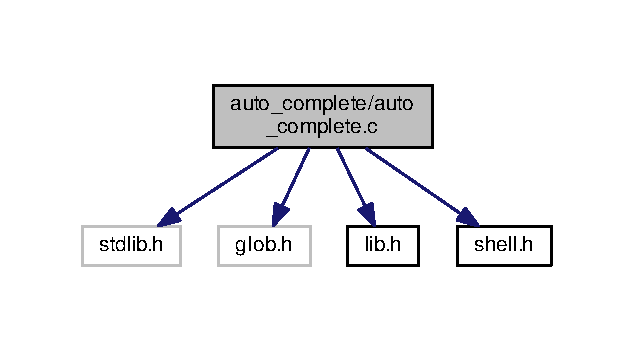
\includegraphics[width=304pt]{auto__complete_8c__incl}
\end{center}
\end{figure}
\subsection*{Functions}
\begin{DoxyCompactItemize}
\item 
char $\ast$ {\bf auto\-\_\-complete} (char $\ast$str)
\end{DoxyCompactItemize}


\subsection{Function Documentation}
\index{auto\-\_\-complete.\-c@{auto\-\_\-complete.\-c}!auto\-\_\-complete@{auto\-\_\-complete}}
\index{auto\-\_\-complete@{auto\-\_\-complete}!auto_complete.c@{auto\-\_\-complete.\-c}}
\subsubsection[{auto\-\_\-complete}]{\setlength{\rightskip}{0pt plus 5cm}char$\ast$ auto\-\_\-complete (
\begin{DoxyParamCaption}
\item[{char $\ast$}]{str}
\end{DoxyParamCaption}
)}\label{auto__complete_8c_a9db47b33aabb3abb191c33e9bc38b173}


Definition at line 57 of file auto\-\_\-complete.\-c.



Here is the call graph for this function\-:\nopagebreak
\begin{figure}[H]
\begin{center}
\leavevmode
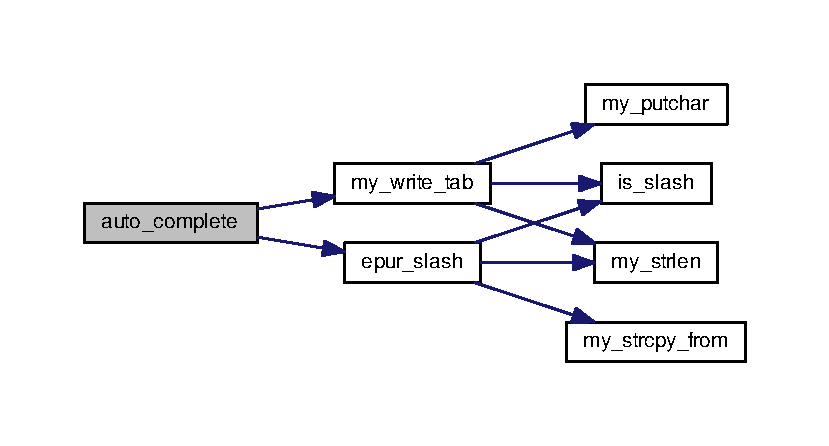
\includegraphics[width=350pt]{auto__complete_8c_a9db47b33aabb3abb191c33e9bc38b173_cgraph}
\end{center}
\end{figure}




Here is the caller graph for this function\-:
\nopagebreak
\begin{figure}[H]
\begin{center}
\leavevmode
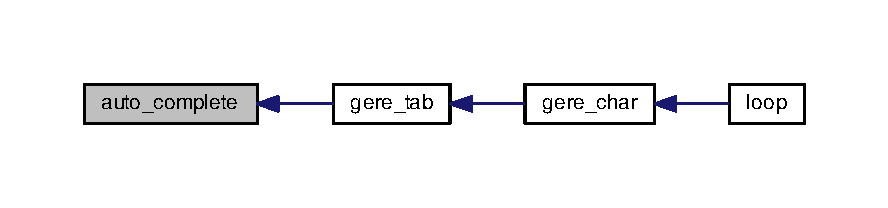
\includegraphics[width=350pt]{auto__complete_8c_a9db47b33aabb3abb191c33e9bc38b173_icgraph}
\end{center}
\end{figure}



\section{auto\-\_\-complete/functions\-\_\-complete.c File Reference}
\label{functions__complete_8c}\index{auto\-\_\-complete/functions\-\_\-complete.\-c@{auto\-\_\-complete/functions\-\_\-complete.\-c}}
{\ttfamily \#include $<$stdlib.\-h$>$}\\*
{\ttfamily \#include \char`\"{}lib.\-h\char`\"{}}\\*
{\ttfamily \#include \char`\"{}shell.\-h\char`\"{}}\\*
Include dependency graph for functions\-\_\-complete.\-c\-:\nopagebreak
\begin{figure}[H]
\begin{center}
\leavevmode
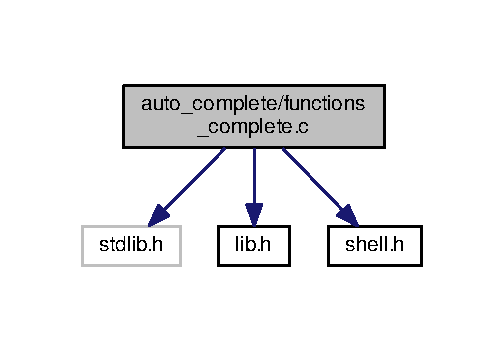
\includegraphics[width=242pt]{functions__complete_8c__incl}
\end{center}
\end{figure}
\subsection*{Functions}
\begin{DoxyCompactItemize}
\item 
int {\bf is\-\_\-slash} (char $\ast$str)
\item 
char $\ast$ {\bf epur\-\_\-slash} (char $\ast$str)
\item 
void {\bf my\-\_\-write\-\_\-tab} (char $\ast$$\ast$tab)
\end{DoxyCompactItemize}


\subsection{Function Documentation}
\index{functions\-\_\-complete.\-c@{functions\-\_\-complete.\-c}!epur\-\_\-slash@{epur\-\_\-slash}}
\index{epur\-\_\-slash@{epur\-\_\-slash}!functions_complete.c@{functions\-\_\-complete.\-c}}
\subsubsection[{epur\-\_\-slash}]{\setlength{\rightskip}{0pt plus 5cm}char$\ast$ epur\-\_\-slash (
\begin{DoxyParamCaption}
\item[{char $\ast$}]{str}
\end{DoxyParamCaption}
)}\label{functions__complete_8c_a0561ce09429ac571427c7b77a61aaed8}


Definition at line 29 of file functions\-\_\-complete.\-c.



Here is the call graph for this function\-:\nopagebreak
\begin{figure}[H]
\begin{center}
\leavevmode
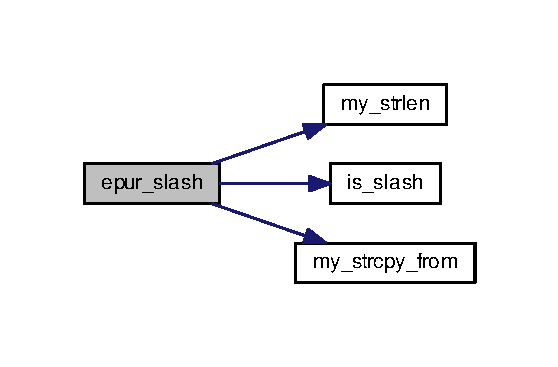
\includegraphics[width=268pt]{functions__complete_8c_a0561ce09429ac571427c7b77a61aaed8_cgraph}
\end{center}
\end{figure}




Here is the caller graph for this function\-:
\nopagebreak
\begin{figure}[H]
\begin{center}
\leavevmode
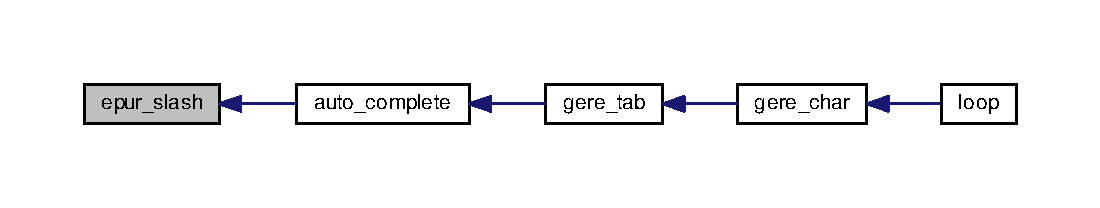
\includegraphics[width=350pt]{functions__complete_8c_a0561ce09429ac571427c7b77a61aaed8_icgraph}
\end{center}
\end{figure}


\index{functions\-\_\-complete.\-c@{functions\-\_\-complete.\-c}!is\-\_\-slash@{is\-\_\-slash}}
\index{is\-\_\-slash@{is\-\_\-slash}!functions_complete.c@{functions\-\_\-complete.\-c}}
\subsubsection[{is\-\_\-slash}]{\setlength{\rightskip}{0pt plus 5cm}int is\-\_\-slash (
\begin{DoxyParamCaption}
\item[{char $\ast$}]{str}
\end{DoxyParamCaption}
)}\label{functions__complete_8c_a43aaf009c1f4a148004ee8cf4f4c5a5a}


Definition at line 15 of file functions\-\_\-complete.\-c.



Here is the caller graph for this function\-:
\nopagebreak
\begin{figure}[H]
\begin{center}
\leavevmode
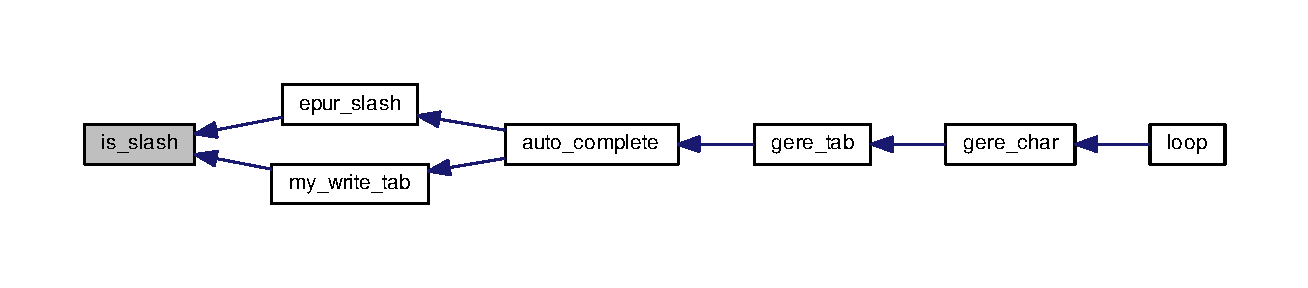
\includegraphics[width=350pt]{functions__complete_8c_a43aaf009c1f4a148004ee8cf4f4c5a5a_icgraph}
\end{center}
\end{figure}


\index{functions\-\_\-complete.\-c@{functions\-\_\-complete.\-c}!my\-\_\-write\-\_\-tab@{my\-\_\-write\-\_\-tab}}
\index{my\-\_\-write\-\_\-tab@{my\-\_\-write\-\_\-tab}!functions_complete.c@{functions\-\_\-complete.\-c}}
\subsubsection[{my\-\_\-write\-\_\-tab}]{\setlength{\rightskip}{0pt plus 5cm}void my\-\_\-write\-\_\-tab (
\begin{DoxyParamCaption}
\item[{char $\ast$$\ast$}]{tab}
\end{DoxyParamCaption}
)}\label{functions__complete_8c_aac577fdfca82ccd407b2105d39b56fce}


Definition at line 48 of file functions\-\_\-complete.\-c.



Here is the call graph for this function\-:\nopagebreak
\begin{figure}[H]
\begin{center}
\leavevmode
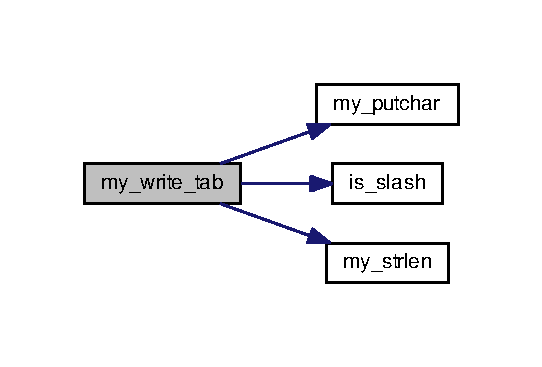
\includegraphics[width=260pt]{functions__complete_8c_aac577fdfca82ccd407b2105d39b56fce_cgraph}
\end{center}
\end{figure}




Here is the caller graph for this function\-:
\nopagebreak
\begin{figure}[H]
\begin{center}
\leavevmode
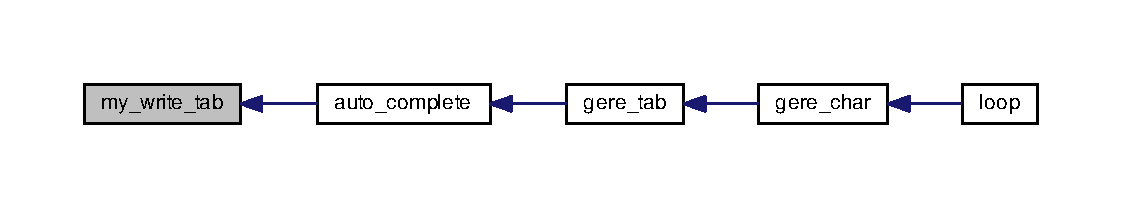
\includegraphics[width=350pt]{functions__complete_8c_aac577fdfca82ccd407b2105d39b56fce_icgraph}
\end{center}
\end{figure}



\section{builtin/builtin.c File Reference}
\label{builtin_8c}\index{builtin/builtin.\-c@{builtin/builtin.\-c}}
{\ttfamily \#include $<$stdio.\-h$>$}\\*
{\ttfamily \#include $<$stdlib.\-h$>$}\\*
{\ttfamily \#include \char`\"{}builtin.\-h\char`\"{}}\\*
{\ttfamily \#include \char`\"{}lib.\-h\char`\"{}}\\*
Include dependency graph for builtin.\-c\-:
\nopagebreak
\begin{figure}[H]
\begin{center}
\leavevmode
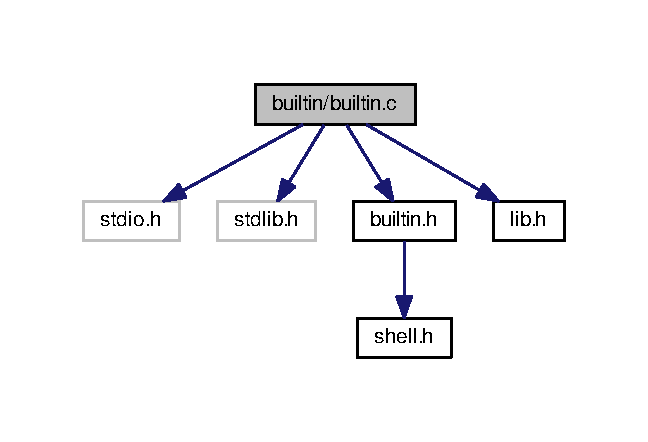
\includegraphics[width=311pt]{builtin_8c__incl}
\end{center}
\end{figure}
\subsection*{Functions}
\begin{DoxyCompactItemize}
\item 
int {\bf my\-\_\-unsetenv} (char $\ast$$\ast$expr, {\bf t\-\_\-data} $\ast$data)
\item 
int {\bf my\-\_\-setenv} (char $\ast$$\ast$expr, {\bf t\-\_\-data} $\ast$data)
\item 
int {\bf my\-\_\-env} (char $\ast$$\ast$expr, {\bf t\-\_\-data} $\ast$data)
\item 
int {\bf my\-\_\-exit} (char $\ast$$\ast$expr, {\bf t\-\_\-data} $\ast$data)
\item 
int {\bf my\-\_\-echo} (char $\ast$$\ast$expr, {\bf t\-\_\-data} $\ast$data)
\end{DoxyCompactItemize}


\subsection{Function Documentation}
\index{builtin.\-c@{builtin.\-c}!my\-\_\-echo@{my\-\_\-echo}}
\index{my\-\_\-echo@{my\-\_\-echo}!builtin.c@{builtin.\-c}}
\subsubsection[{my\-\_\-echo}]{\setlength{\rightskip}{0pt plus 5cm}int my\-\_\-echo (
\begin{DoxyParamCaption}
\item[{char $\ast$$\ast$}]{expr, }
\item[{{\bf t\-\_\-data} $\ast$}]{data}
\end{DoxyParamCaption}
)}\label{builtin_8c_a95a62fb319cfd787bd672b23b9288c67}


Definition at line 101 of file builtin.\-c.



Here is the call graph for this function\-:
\nopagebreak
\begin{figure}[H]
\begin{center}
\leavevmode
\includegraphics[width=350pt]{builtin_8c_a95a62fb319cfd787bd672b23b9288c67_cgraph}
\end{center}
\end{figure}




Here is the caller graph for this function\-:
\nopagebreak
\begin{figure}[H]
\begin{center}
\leavevmode
\includegraphics[width=350pt]{builtin_8c_a95a62fb319cfd787bd672b23b9288c67_icgraph}
\end{center}
\end{figure}


\index{builtin.\-c@{builtin.\-c}!my\-\_\-env@{my\-\_\-env}}
\index{my\-\_\-env@{my\-\_\-env}!builtin.c@{builtin.\-c}}
\subsubsection[{my\-\_\-env}]{\setlength{\rightskip}{0pt plus 5cm}int my\-\_\-env (
\begin{DoxyParamCaption}
\item[{char $\ast$$\ast$}]{expr, }
\item[{{\bf t\-\_\-data} $\ast$}]{data}
\end{DoxyParamCaption}
)}\label{builtin_8c_a8608a65d45d2d3d7ec0e83a91d1f51a3}


Definition at line 71 of file builtin.\-c.



Here is the call graph for this function\-:
\nopagebreak
\begin{figure}[H]
\begin{center}
\leavevmode
\includegraphics[width=234pt]{builtin_8c_a8608a65d45d2d3d7ec0e83a91d1f51a3_cgraph}
\end{center}
\end{figure}




Here is the caller graph for this function\-:
\nopagebreak
\begin{figure}[H]
\begin{center}
\leavevmode
\includegraphics[width=350pt]{builtin_8c_a8608a65d45d2d3d7ec0e83a91d1f51a3_icgraph}
\end{center}
\end{figure}


\index{builtin.\-c@{builtin.\-c}!my\-\_\-exit@{my\-\_\-exit}}
\index{my\-\_\-exit@{my\-\_\-exit}!builtin.c@{builtin.\-c}}
\subsubsection[{my\-\_\-exit}]{\setlength{\rightskip}{0pt plus 5cm}int my\-\_\-exit (
\begin{DoxyParamCaption}
\item[{char $\ast$$\ast$}]{expr, }
\item[{{\bf t\-\_\-data} $\ast$}]{data}
\end{DoxyParamCaption}
)}\label{builtin_8c_a3f937a32f761532cf83be2cd3dae0e09}


Definition at line 92 of file builtin.\-c.



Here is the call graph for this function\-:\nopagebreak
\begin{figure}[H]
\begin{center}
\leavevmode
\includegraphics[width=350pt]{builtin_8c_a3f937a32f761532cf83be2cd3dae0e09_cgraph}
\end{center}
\end{figure}




Here is the caller graph for this function\-:
\nopagebreak
\begin{figure}[H]
\begin{center}
\leavevmode
\includegraphics[width=350pt]{builtin_8c_a3f937a32f761532cf83be2cd3dae0e09_icgraph}
\end{center}
\end{figure}


\index{builtin.\-c@{builtin.\-c}!my\-\_\-setenv@{my\-\_\-setenv}}
\index{my\-\_\-setenv@{my\-\_\-setenv}!builtin.c@{builtin.\-c}}
\subsubsection[{my\-\_\-setenv}]{\setlength{\rightskip}{0pt plus 5cm}int my\-\_\-setenv (
\begin{DoxyParamCaption}
\item[{char $\ast$$\ast$}]{expr, }
\item[{{\bf t\-\_\-data} $\ast$}]{data}
\end{DoxyParamCaption}
)}\label{builtin_8c_aa3ae54ee16af4313f2ccb3c2fff447e9}


Definition at line 44 of file builtin.\-c.



Here is the call graph for this function\-:\nopagebreak
\begin{figure}[H]
\begin{center}
\leavevmode
\includegraphics[width=350pt]{builtin_8c_aa3ae54ee16af4313f2ccb3c2fff447e9_cgraph}
\end{center}
\end{figure}




Here is the caller graph for this function\-:
\nopagebreak
\begin{figure}[H]
\begin{center}
\leavevmode
\includegraphics[width=350pt]{builtin_8c_aa3ae54ee16af4313f2ccb3c2fff447e9_icgraph}
\end{center}
\end{figure}


\index{builtin.\-c@{builtin.\-c}!my\-\_\-unsetenv@{my\-\_\-unsetenv}}
\index{my\-\_\-unsetenv@{my\-\_\-unsetenv}!builtin.c@{builtin.\-c}}
\subsubsection[{my\-\_\-unsetenv}]{\setlength{\rightskip}{0pt plus 5cm}int my\-\_\-unsetenv (
\begin{DoxyParamCaption}
\item[{char $\ast$$\ast$}]{expr, }
\item[{{\bf t\-\_\-data} $\ast$}]{data}
\end{DoxyParamCaption}
)}\label{builtin_8c_a7bd51fb3b758ec7342192213355ec102}


Definition at line 16 of file builtin.\-c.



Here is the call graph for this function\-:\nopagebreak
\begin{figure}[H]
\begin{center}
\leavevmode
\includegraphics[width=276pt]{builtin_8c_a7bd51fb3b758ec7342192213355ec102_cgraph}
\end{center}
\end{figure}




Here is the caller graph for this function\-:
\nopagebreak
\begin{figure}[H]
\begin{center}
\leavevmode
\includegraphics[width=350pt]{builtin_8c_a7bd51fb3b758ec7342192213355ec102_icgraph}
\end{center}
\end{figure}



\section{builtin/cd.c File Reference}
\label{cd_8c}\index{builtin/cd.\-c@{builtin/cd.\-c}}
{\ttfamily \#include $<$stdio.\-h$>$}\\*
{\ttfamily \#include $<$string.\-h$>$}\\*
{\ttfamily \#include $<$stdlib.\-h$>$}\\*
{\ttfamily \#include $<$unistd.\-h$>$}\\*
{\ttfamily \#include \char`\"{}builtin.\-h\char`\"{}}\\*
{\ttfamily \#include \char`\"{}lib.\-h\char`\"{}}\\*
Include dependency graph for cd.\-c\-:
\nopagebreak
\begin{figure}[H]
\begin{center}
\leavevmode
\includegraphics[width=350pt]{cd_8c__incl}
\end{center}
\end{figure}
\subsection*{Functions}
\begin{DoxyCompactItemize}
\item 
int {\bf my\-\_\-cd\-\_\-error} (char $\ast$str)
\item 
char $\ast$ {\bf get\-\_\-new\-\_\-pwd} (char $\ast$pwd, char $\ast$path)
\item 
int {\bf set\-\_\-pwd\-\_\-old\-\_\-pwd} (char $\ast$$\ast$env, char $\ast$path)
\item 
int {\bf my\-\_\-cd} (char $\ast$$\ast$expr, {\bf t\-\_\-data} $\ast$data)
\end{DoxyCompactItemize}


\subsection{Function Documentation}
\index{cd.\-c@{cd.\-c}!get\-\_\-new\-\_\-pwd@{get\-\_\-new\-\_\-pwd}}
\index{get\-\_\-new\-\_\-pwd@{get\-\_\-new\-\_\-pwd}!cd.c@{cd.\-c}}
\subsubsection[{get\-\_\-new\-\_\-pwd}]{\setlength{\rightskip}{0pt plus 5cm}char$\ast$ get\-\_\-new\-\_\-pwd (
\begin{DoxyParamCaption}
\item[{char $\ast$}]{pwd, }
\item[{char $\ast$}]{path}
\end{DoxyParamCaption}
)}\label{cd_8c_af74884482c27a5e006206669ebbd5b8e}


Definition at line 24 of file cd.\-c.



Here is the call graph for this function\-:
\nopagebreak
\begin{figure}[H]
\begin{center}
\leavevmode
\includegraphics[width=350pt]{cd_8c_af74884482c27a5e006206669ebbd5b8e_cgraph}
\end{center}
\end{figure}




Here is the caller graph for this function\-:
\nopagebreak
\begin{figure}[H]
\begin{center}
\leavevmode
\includegraphics[width=350pt]{cd_8c_af74884482c27a5e006206669ebbd5b8e_icgraph}
\end{center}
\end{figure}


\index{cd.\-c@{cd.\-c}!my\-\_\-cd@{my\-\_\-cd}}
\index{my\-\_\-cd@{my\-\_\-cd}!cd.c@{cd.\-c}}
\subsubsection[{my\-\_\-cd}]{\setlength{\rightskip}{0pt plus 5cm}int my\-\_\-cd (
\begin{DoxyParamCaption}
\item[{char $\ast$$\ast$}]{expr, }
\item[{{\bf t\-\_\-data} $\ast$}]{data}
\end{DoxyParamCaption}
)}\label{cd_8c_a04d617582a090298a993bb56e5a66cb9}


Definition at line 73 of file cd.\-c.



Here is the call graph for this function\-:
\nopagebreak
\begin{figure}[H]
\begin{center}
\leavevmode
\includegraphics[width=350pt]{cd_8c_a04d617582a090298a993bb56e5a66cb9_cgraph}
\end{center}
\end{figure}




Here is the caller graph for this function\-:
\nopagebreak
\begin{figure}[H]
\begin{center}
\leavevmode
\includegraphics[width=350pt]{cd_8c_a04d617582a090298a993bb56e5a66cb9_icgraph}
\end{center}
\end{figure}


\index{cd.\-c@{cd.\-c}!my\-\_\-cd\-\_\-error@{my\-\_\-cd\-\_\-error}}
\index{my\-\_\-cd\-\_\-error@{my\-\_\-cd\-\_\-error}!cd.c@{cd.\-c}}
\subsubsection[{my\-\_\-cd\-\_\-error}]{\setlength{\rightskip}{0pt plus 5cm}int my\-\_\-cd\-\_\-error (
\begin{DoxyParamCaption}
\item[{char $\ast$}]{str}
\end{DoxyParamCaption}
)}\label{cd_8c_a27ff54b856199cbd22e0983f4b369f6b}


Definition at line 18 of file cd.\-c.



Here is the caller graph for this function\-:
\nopagebreak
\begin{figure}[H]
\begin{center}
\leavevmode
\includegraphics[width=350pt]{cd_8c_a27ff54b856199cbd22e0983f4b369f6b_icgraph}
\end{center}
\end{figure}


\index{cd.\-c@{cd.\-c}!set\-\_\-pwd\-\_\-old\-\_\-pwd@{set\-\_\-pwd\-\_\-old\-\_\-pwd}}
\index{set\-\_\-pwd\-\_\-old\-\_\-pwd@{set\-\_\-pwd\-\_\-old\-\_\-pwd}!cd.c@{cd.\-c}}
\subsubsection[{set\-\_\-pwd\-\_\-old\-\_\-pwd}]{\setlength{\rightskip}{0pt plus 5cm}int set\-\_\-pwd\-\_\-old\-\_\-pwd (
\begin{DoxyParamCaption}
\item[{char $\ast$$\ast$}]{env, }
\item[{char $\ast$}]{path}
\end{DoxyParamCaption}
)}\label{cd_8c_adff71582669f5726a87d35e9f9a15057}


Definition at line 53 of file cd.\-c.



Here is the call graph for this function\-:
\nopagebreak
\begin{figure}[H]
\begin{center}
\leavevmode
\includegraphics[width=350pt]{cd_8c_adff71582669f5726a87d35e9f9a15057_cgraph}
\end{center}
\end{figure}




Here is the caller graph for this function\-:
\nopagebreak
\begin{figure}[H]
\begin{center}
\leavevmode
\includegraphics[width=350pt]{cd_8c_adff71582669f5726a87d35e9f9a15057_icgraph}
\end{center}
\end{figure}



\section{builtin/forbuiltin.c File Reference}
\label{forbuiltin_8c}\index{builtin/forbuiltin.\-c@{builtin/forbuiltin.\-c}}
{\ttfamily \#include $<$string.\-h$>$}\\*
{\ttfamily \#include $<$unistd.\-h$>$}\\*
{\ttfamily \#include $<$stdlib.\-h$>$}\\*
{\ttfamily \#include \char`\"{}builtin.\-h\char`\"{}}\\*
{\ttfamily \#include \char`\"{}lib.\-h\char`\"{}}\\*
Include dependency graph for forbuiltin.\-c\-:\nopagebreak
\begin{figure}[H]
\begin{center}
\leavevmode
\includegraphics[width=350pt]{forbuiltin_8c__incl}
\end{center}
\end{figure}
\subsection*{Functions}
\begin{DoxyCompactItemize}
\item 
void {\bf other\-\_\-echo\-\_\-case} (char $\ast$str, int $\ast$i, char done)
\item 
int {\bf my\-\_\-interpret} (char $\ast$str, int i, int k, char done)
\item 
int {\bf my\-\_\-print} (char $\ast$str, char inter, char noret, char $\ast$nextword)
\item 
char $\ast$$\ast$ {\bf my\-\_\-epurtab} (char $\ast$$\ast$tab)
\item 
char $\ast$$\ast$ {\bf my\-\_\-cattab} (char $\ast$$\ast$tab, char $\ast$new)
\end{DoxyCompactItemize}
\subsection*{Variables}
\begin{DoxyCompactItemize}
\item 
char {\bf g\-\_\-ref} [8][2]
\end{DoxyCompactItemize}


\subsection{Function Documentation}
\index{forbuiltin.\-c@{forbuiltin.\-c}!my\-\_\-cattab@{my\-\_\-cattab}}
\index{my\-\_\-cattab@{my\-\_\-cattab}!forbuiltin.c@{forbuiltin.\-c}}
\subsubsection[{my\-\_\-cattab}]{\setlength{\rightskip}{0pt plus 5cm}char$\ast$$\ast$ my\-\_\-cattab (
\begin{DoxyParamCaption}
\item[{char $\ast$$\ast$}]{tab, }
\item[{char $\ast$}]{new}
\end{DoxyParamCaption}
)}\label{forbuiltin_8c_a795c38158cb00f9fcad0dd7db17e7ded}


Definition at line 124 of file forbuiltin.\-c.



Here is the call graph for this function\-:\nopagebreak
\begin{figure}[H]
\begin{center}
\leavevmode
\includegraphics[width=240pt]{forbuiltin_8c_a795c38158cb00f9fcad0dd7db17e7ded_cgraph}
\end{center}
\end{figure}




Here is the caller graph for this function\-:
\nopagebreak
\begin{figure}[H]
\begin{center}
\leavevmode
\includegraphics[width=350pt]{forbuiltin_8c_a795c38158cb00f9fcad0dd7db17e7ded_icgraph}
\end{center}
\end{figure}


\index{forbuiltin.\-c@{forbuiltin.\-c}!my\-\_\-epurtab@{my\-\_\-epurtab}}
\index{my\-\_\-epurtab@{my\-\_\-epurtab}!forbuiltin.c@{forbuiltin.\-c}}
\subsubsection[{my\-\_\-epurtab}]{\setlength{\rightskip}{0pt plus 5cm}char$\ast$$\ast$ my\-\_\-epurtab (
\begin{DoxyParamCaption}
\item[{char $\ast$$\ast$}]{tab}
\end{DoxyParamCaption}
)}\label{forbuiltin_8c_a9c81bd03dd1d5eae7cee8720ff4a4f25}


Definition at line 95 of file forbuiltin.\-c.



Here is the caller graph for this function\-:
\nopagebreak
\begin{figure}[H]
\begin{center}
\leavevmode
\includegraphics[width=350pt]{forbuiltin_8c_a9c81bd03dd1d5eae7cee8720ff4a4f25_icgraph}
\end{center}
\end{figure}


\index{forbuiltin.\-c@{forbuiltin.\-c}!my\-\_\-interpret@{my\-\_\-interpret}}
\index{my\-\_\-interpret@{my\-\_\-interpret}!forbuiltin.c@{forbuiltin.\-c}}
\subsubsection[{my\-\_\-interpret}]{\setlength{\rightskip}{0pt plus 5cm}int my\-\_\-interpret (
\begin{DoxyParamCaption}
\item[{char $\ast$}]{str, }
\item[{int}]{i, }
\item[{int}]{k, }
\item[{char}]{done}
\end{DoxyParamCaption}
)}\label{forbuiltin_8c_abd901da92b9ba2506b04b5c3a640bba2}


Definition at line 43 of file forbuiltin.\-c.



Here is the call graph for this function\-:\nopagebreak
\begin{figure}[H]
\begin{center}
\leavevmode
\includegraphics[width=350pt]{forbuiltin_8c_abd901da92b9ba2506b04b5c3a640bba2_cgraph}
\end{center}
\end{figure}




Here is the caller graph for this function\-:
\nopagebreak
\begin{figure}[H]
\begin{center}
\leavevmode
\includegraphics[width=350pt]{forbuiltin_8c_abd901da92b9ba2506b04b5c3a640bba2_icgraph}
\end{center}
\end{figure}


\index{forbuiltin.\-c@{forbuiltin.\-c}!my\-\_\-print@{my\-\_\-print}}
\index{my\-\_\-print@{my\-\_\-print}!forbuiltin.c@{forbuiltin.\-c}}
\subsubsection[{my\-\_\-print}]{\setlength{\rightskip}{0pt plus 5cm}int my\-\_\-print (
\begin{DoxyParamCaption}
\item[{char $\ast$}]{str, }
\item[{char}]{inter, }
\item[{char}]{noret, }
\item[{char $\ast$}]{nextword}
\end{DoxyParamCaption}
)}\label{forbuiltin_8c_a3da96f75f1c99d390ce5582d73f7bf18}


Definition at line 72 of file forbuiltin.\-c.



Here is the call graph for this function\-:\nopagebreak
\begin{figure}[H]
\begin{center}
\leavevmode
\includegraphics[width=350pt]{forbuiltin_8c_a3da96f75f1c99d390ce5582d73f7bf18_cgraph}
\end{center}
\end{figure}




Here is the caller graph for this function\-:
\nopagebreak
\begin{figure}[H]
\begin{center}
\leavevmode
\includegraphics[width=350pt]{forbuiltin_8c_a3da96f75f1c99d390ce5582d73f7bf18_icgraph}
\end{center}
\end{figure}


\index{forbuiltin.\-c@{forbuiltin.\-c}!other\-\_\-echo\-\_\-case@{other\-\_\-echo\-\_\-case}}
\index{other\-\_\-echo\-\_\-case@{other\-\_\-echo\-\_\-case}!forbuiltin.c@{forbuiltin.\-c}}
\subsubsection[{other\-\_\-echo\-\_\-case}]{\setlength{\rightskip}{0pt plus 5cm}void other\-\_\-echo\-\_\-case (
\begin{DoxyParamCaption}
\item[{char $\ast$}]{str, }
\item[{int $\ast$}]{i, }
\item[{char}]{done}
\end{DoxyParamCaption}
)}\label{forbuiltin_8c_af3d3a3e1f2acbf9eccc05028b283bbb6}


Definition at line 26 of file forbuiltin.\-c.



Here is the call graph for this function\-:\nopagebreak
\begin{figure}[H]
\begin{center}
\leavevmode
\includegraphics[width=304pt]{forbuiltin_8c_af3d3a3e1f2acbf9eccc05028b283bbb6_cgraph}
\end{center}
\end{figure}




Here is the caller graph for this function\-:
\nopagebreak
\begin{figure}[H]
\begin{center}
\leavevmode
\includegraphics[width=350pt]{forbuiltin_8c_af3d3a3e1f2acbf9eccc05028b283bbb6_icgraph}
\end{center}
\end{figure}




\subsection{Variable Documentation}
\index{forbuiltin.\-c@{forbuiltin.\-c}!g\-\_\-ref@{g\-\_\-ref}}
\index{g\-\_\-ref@{g\-\_\-ref}!forbuiltin.c@{forbuiltin.\-c}}
\subsubsection[{g\-\_\-ref}]{\setlength{\rightskip}{0pt plus 5cm}char g\-\_\-ref[8][2]}\label{forbuiltin_8c_a8ca280e502460ed6510ec75af0321d03}
{\bfseries Initial value\-:}
\begin{DoxyCode}
= \{\{\textcolor{charliteral}{'a'}, \textcolor{charliteral}{'\(\backslash\)a'}\},
               \{\textcolor{charliteral}{'b'}, \textcolor{charliteral}{'\(\backslash\)b'}\},
               \{\textcolor{charliteral}{'e'}, ESCAPE\},
               \{\textcolor{charliteral}{'f'}, \textcolor{charliteral}{'\(\backslash\)f'}\},
               \{\textcolor{charliteral}{'n'}, \textcolor{charliteral}{'\(\backslash\)n'}\},
               \{\textcolor{charliteral}{'r'}, \textcolor{charliteral}{'\(\backslash\)r'}\},
               \{\textcolor{charliteral}{'t'}, \textcolor{charliteral}{'\(\backslash\)t'}\},
               \{\textcolor{charliteral}{'v'}, \textcolor{charliteral}{'\(\backslash\)v'}\}\}
\end{DoxyCode}


Definition at line 17 of file forbuiltin.\-c.


\section{builtin/getvar.c File Reference}
\label{getvar_8c}\index{builtin/getvar.\-c@{builtin/getvar.\-c}}
{\ttfamily \#include $<$stdlib.\-h$>$}\\*
{\ttfamily \#include $<$lib.\-h$>$}\\*
{\ttfamily \#include \char`\"{}builtin.\-h\char`\"{}}\\*
Include dependency graph for getvar.\-c\-:\nopagebreak
\begin{figure}[H]
\begin{center}
\leavevmode
\includegraphics[width=246pt]{getvar_8c__incl}
\end{center}
\end{figure}
\subsection*{Functions}
\begin{DoxyCompactItemize}
\item 
void {\bf delete\-\_\-first\-\_\-word} (char $\ast$$\ast$wtab)
\item 
int {\bf my\-\_\-replace\-\_\-key} (char $\ast$$\ast$expr, {\bf t\-\_\-data} $\ast$data)
\item 
char $\ast$ {\bf my\-\_\-cstrconcat} (char $\ast$s1, char $\ast$s2)
\end{DoxyCompactItemize}


\subsection{Function Documentation}
\index{getvar.\-c@{getvar.\-c}!delete\-\_\-first\-\_\-word@{delete\-\_\-first\-\_\-word}}
\index{delete\-\_\-first\-\_\-word@{delete\-\_\-first\-\_\-word}!getvar.c@{getvar.\-c}}
\subsubsection[{delete\-\_\-first\-\_\-word}]{\setlength{\rightskip}{0pt plus 5cm}void delete\-\_\-first\-\_\-word (
\begin{DoxyParamCaption}
\item[{char $\ast$$\ast$}]{wtab}
\end{DoxyParamCaption}
)}\label{getvar_8c_a31f8c796cea615093b779b9e32db6d02}


Definition at line 15 of file getvar.\-c.



Here is the caller graph for this function\-:
\nopagebreak
\begin{figure}[H]
\begin{center}
\leavevmode
\includegraphics[width=350pt]{getvar_8c_a31f8c796cea615093b779b9e32db6d02_icgraph}
\end{center}
\end{figure}


\index{getvar.\-c@{getvar.\-c}!my\-\_\-cstrconcat@{my\-\_\-cstrconcat}}
\index{my\-\_\-cstrconcat@{my\-\_\-cstrconcat}!getvar.c@{getvar.\-c}}
\subsubsection[{my\-\_\-cstrconcat}]{\setlength{\rightskip}{0pt plus 5cm}char$\ast$ my\-\_\-cstrconcat (
\begin{DoxyParamCaption}
\item[{char $\ast$}]{s1, }
\item[{char $\ast$}]{s2}
\end{DoxyParamCaption}
)}\label{getvar_8c_a2883a48551d7c810ebd592fb241efeed}


Definition at line 50 of file getvar.\-c.



Here is the call graph for this function\-:\nopagebreak
\begin{figure}[H]
\begin{center}
\leavevmode
\includegraphics[width=258pt]{getvar_8c_a2883a48551d7c810ebd592fb241efeed_cgraph}
\end{center}
\end{figure}




Here is the caller graph for this function\-:
\nopagebreak
\begin{figure}[H]
\begin{center}
\leavevmode
\includegraphics[width=350pt]{getvar_8c_a2883a48551d7c810ebd592fb241efeed_icgraph}
\end{center}
\end{figure}


\index{getvar.\-c@{getvar.\-c}!my\-\_\-replace\-\_\-key@{my\-\_\-replace\-\_\-key}}
\index{my\-\_\-replace\-\_\-key@{my\-\_\-replace\-\_\-key}!getvar.c@{getvar.\-c}}
\subsubsection[{my\-\_\-replace\-\_\-key}]{\setlength{\rightskip}{0pt plus 5cm}int my\-\_\-replace\-\_\-key (
\begin{DoxyParamCaption}
\item[{char $\ast$$\ast$}]{expr, }
\item[{{\bf t\-\_\-data} $\ast$}]{data}
\end{DoxyParamCaption}
)}\label{getvar_8c_a6055c5e4f8247c5a1151cd65e5061574}


Definition at line 28 of file getvar.\-c.



Here is the call graph for this function\-:\nopagebreak
\begin{figure}[H]
\begin{center}
\leavevmode
\includegraphics[width=302pt]{getvar_8c_a6055c5e4f8247c5a1151cd65e5061574_cgraph}
\end{center}
\end{figure}




Here is the caller graph for this function\-:
\nopagebreak
\begin{figure}[H]
\begin{center}
\leavevmode
\includegraphics[width=350pt]{getvar_8c_a6055c5e4f8247c5a1151cd65e5061574_icgraph}
\end{center}
\end{figure}



\section{builtin/top\-\_\-builtin.c File Reference}
\label{top__builtin_8c}\index{builtin/top\-\_\-builtin.\-c@{builtin/top\-\_\-builtin.\-c}}
{\ttfamily \#include $<$stdlib.\-h$>$}\\*
{\ttfamily \#include $<$string.\-h$>$}\\*
{\ttfamily \#include $<$unistd.\-h$>$}\\*
{\ttfamily \#include \char`\"{}builtin.\-h\char`\"{}}\\*
Include dependency graph for top\-\_\-builtin.\-c\-:
\nopagebreak
\begin{figure}[H]
\begin{center}
\leavevmode
\includegraphics[width=328pt]{top__builtin_8c__incl}
\end{center}
\end{figure}
\subsection*{Functions}
\begin{DoxyCompactItemize}
\item 
int {\bf my\-\_\-redir\-\_\-builtin} ({\bf t\-\_\-data} $\ast$data, {\bf t\-\_\-cmd} $\ast$cmd)
\item 
int {\bf builtin} ({\bf t\-\_\-data} $\ast$data, char $\ast$$\ast$cmd)
\end{DoxyCompactItemize}


\subsection{Function Documentation}
\index{top\-\_\-builtin.\-c@{top\-\_\-builtin.\-c}!builtin@{builtin}}
\index{builtin@{builtin}!top_builtin.c@{top\-\_\-builtin.\-c}}
\subsubsection[{builtin}]{\setlength{\rightskip}{0pt plus 5cm}int builtin (
\begin{DoxyParamCaption}
\item[{{\bf t\-\_\-data} $\ast$}]{data, }
\item[{char $\ast$$\ast$}]{cmd}
\end{DoxyParamCaption}
)}\label{top__builtin_8c_a4a932a3567484ecc159fb43f41392992}


Definition at line 35 of file top\-\_\-builtin.\-c.



Here is the call graph for this function\-:
\nopagebreak
\begin{figure}[H]
\begin{center}
\leavevmode
\includegraphics[width=350pt]{top__builtin_8c_a4a932a3567484ecc159fb43f41392992_cgraph}
\end{center}
\end{figure}




Here is the caller graph for this function\-:
\nopagebreak
\begin{figure}[H]
\begin{center}
\leavevmode
\includegraphics[width=350pt]{top__builtin_8c_a4a932a3567484ecc159fb43f41392992_icgraph}
\end{center}
\end{figure}


\index{top\-\_\-builtin.\-c@{top\-\_\-builtin.\-c}!my\-\_\-redir\-\_\-builtin@{my\-\_\-redir\-\_\-builtin}}
\index{my\-\_\-redir\-\_\-builtin@{my\-\_\-redir\-\_\-builtin}!top_builtin.c@{top\-\_\-builtin.\-c}}
\subsubsection[{my\-\_\-redir\-\_\-builtin}]{\setlength{\rightskip}{0pt plus 5cm}int my\-\_\-redir\-\_\-builtin (
\begin{DoxyParamCaption}
\item[{{\bf t\-\_\-data} $\ast$}]{data, }
\item[{{\bf t\-\_\-cmd} $\ast$}]{cmd}
\end{DoxyParamCaption}
)}\label{top__builtin_8c_aecb1f227db5bcfc86869d066066f450d}


Definition at line 16 of file top\-\_\-builtin.\-c.



Here is the call graph for this function\-:
\nopagebreak
\begin{figure}[H]
\begin{center}
\leavevmode
\includegraphics[width=350pt]{top__builtin_8c_aecb1f227db5bcfc86869d066066f450d_cgraph}
\end{center}
\end{figure}




Here is the caller graph for this function\-:
\nopagebreak
\begin{figure}[H]
\begin{center}
\leavevmode
\includegraphics[width=350pt]{top__builtin_8c_aecb1f227db5bcfc86869d066066f450d_icgraph}
\end{center}
\end{figure}



\section{builtin/utils.c File Reference}
\label{builtin_2utils_8c}\index{builtin/utils.\-c@{builtin/utils.\-c}}
{\ttfamily \#include $<$string.\-h$>$}\\*
{\ttfamily \#include $<$stdlib.\-h$>$}\\*
Include dependency graph for utils.\-c\-:\nopagebreak
\begin{figure}[H]
\begin{center}
\leavevmode
\includegraphics[width=193pt]{builtin_2utils_8c__incl}
\end{center}
\end{figure}
\subsection*{Functions}
\begin{DoxyCompactItemize}
\item 
int {\bf my\-\_\-getnbr\-\_\-base} (char $\ast$str, char $\ast$base, int $\ast$offset, int i)
\item 
char $\ast$ {\bf get\-\_\-env\-\_\-value} (char $\ast$$\ast$env, char $\ast$key, int $\ast$offset)
\item 
char $\ast$$\ast$ {\bf cattab\-\_\-ext} (char $\ast$new)
\end{DoxyCompactItemize}


\subsection{Function Documentation}
\index{builtin/utils.\-c@{builtin/utils.\-c}!cattab\-\_\-ext@{cattab\-\_\-ext}}
\index{cattab\-\_\-ext@{cattab\-\_\-ext}!builtin/utils.c@{builtin/utils.\-c}}
\subsubsection[{cattab\-\_\-ext}]{\setlength{\rightskip}{0pt plus 5cm}char$\ast$$\ast$ cattab\-\_\-ext (
\begin{DoxyParamCaption}
\item[{char $\ast$}]{new}
\end{DoxyParamCaption}
)}\label{builtin_2utils_8c_ac46a37eeaf4141428d46b5605bbd6c51}


Definition at line 60 of file utils.\-c.



Here is the caller graph for this function\-:
\nopagebreak
\begin{figure}[H]
\begin{center}
\leavevmode
\includegraphics[width=350pt]{builtin_2utils_8c_ac46a37eeaf4141428d46b5605bbd6c51_icgraph}
\end{center}
\end{figure}


\index{builtin/utils.\-c@{builtin/utils.\-c}!get\-\_\-env\-\_\-value@{get\-\_\-env\-\_\-value}}
\index{get\-\_\-env\-\_\-value@{get\-\_\-env\-\_\-value}!builtin/utils.c@{builtin/utils.\-c}}
\subsubsection[{get\-\_\-env\-\_\-value}]{\setlength{\rightskip}{0pt plus 5cm}char$\ast$ get\-\_\-env\-\_\-value (
\begin{DoxyParamCaption}
\item[{char $\ast$$\ast$}]{env, }
\item[{char $\ast$}]{key, }
\item[{int $\ast$}]{offset}
\end{DoxyParamCaption}
)}\label{builtin_2utils_8c_a0059bf9838c7770b46270fedbc869799}


Definition at line 42 of file utils.\-c.



Here is the caller graph for this function\-:
\nopagebreak
\begin{figure}[H]
\begin{center}
\leavevmode
\includegraphics[width=350pt]{builtin_2utils_8c_a0059bf9838c7770b46270fedbc869799_icgraph}
\end{center}
\end{figure}


\index{builtin/utils.\-c@{builtin/utils.\-c}!my\-\_\-getnbr\-\_\-base@{my\-\_\-getnbr\-\_\-base}}
\index{my\-\_\-getnbr\-\_\-base@{my\-\_\-getnbr\-\_\-base}!builtin/utils.c@{builtin/utils.\-c}}
\subsubsection[{my\-\_\-getnbr\-\_\-base}]{\setlength{\rightskip}{0pt plus 5cm}int my\-\_\-getnbr\-\_\-base (
\begin{DoxyParamCaption}
\item[{char $\ast$}]{str, }
\item[{char $\ast$}]{base, }
\item[{int $\ast$}]{offset, }
\item[{int}]{i}
\end{DoxyParamCaption}
)}\label{builtin_2utils_8c_a0bd2485960de353416dedf1cf03a943e}


Definition at line 14 of file utils.\-c.



Here is the caller graph for this function\-:
\nopagebreak
\begin{figure}[H]
\begin{center}
\leavevmode
\includegraphics[width=350pt]{builtin_2utils_8c_a0bd2485960de353416dedf1cf03a943e_icgraph}
\end{center}
\end{figure}



\section{ps1/utils.c File Reference}
\label{ps1_2utils_8c}\index{ps1/utils.\-c@{ps1/utils.\-c}}
{\ttfamily \#include $<$string.\-h$>$}\\*
{\ttfamily \#include \char`\"{}ps1.\-h\char`\"{}}\\*
{\ttfamily \#include \char`\"{}shell.\-h\char`\"{}}\\*
{\ttfamily \#include \char`\"{}builtin.\-h\char`\"{}}\\*
{\ttfamily \#include \char`\"{}lib.\-h\char`\"{}}\\*
Include dependency graph for utils.\-c\-:\nopagebreak
\begin{figure}[H]
\begin{center}
\leavevmode
\includegraphics[width=344pt]{ps1_2utils_8c__incl}
\end{center}
\end{figure}
\subsection*{Functions}
\begin{DoxyCompactItemize}
\item 
void {\bf case\-\_\-beep} (char $\ast$$\ast$env)
\item 
int {\bf launch\-\_\-format} (int $\ast$i, char $\ast$str, char $\ast$$\ast$env)
\item 
int {\bf get\-\_\-ps1} (char $\ast$str, char $\ast$$\ast$env)
\item 
char $\ast$ {\bf fix\-\_\-ps1} (char $\ast$ps1)
\item 
int {\bf pars\-\_\-ps1} (char $\ast$$\ast$env)
\end{DoxyCompactItemize}


\subsection{Function Documentation}
\index{ps1/utils.\-c@{ps1/utils.\-c}!case\-\_\-beep@{case\-\_\-beep}}
\index{case\-\_\-beep@{case\-\_\-beep}!ps1/utils.c@{ps1/utils.\-c}}
\subsubsection[{case\-\_\-beep}]{\setlength{\rightskip}{0pt plus 5cm}void case\-\_\-beep (
\begin{DoxyParamCaption}
\item[{char $\ast$$\ast$}]{env}
\end{DoxyParamCaption}
)}\label{ps1_2utils_8c_a87c542912fe159e4137edfda5b3bda75}


Definition at line 27 of file utils.\-c.



Here is the call graph for this function\-:\nopagebreak
\begin{figure}[H]
\begin{center}
\leavevmode
\includegraphics[width=252pt]{ps1_2utils_8c_a87c542912fe159e4137edfda5b3bda75_cgraph}
\end{center}
\end{figure}


\index{ps1/utils.\-c@{ps1/utils.\-c}!fix\-\_\-ps1@{fix\-\_\-ps1}}
\index{fix\-\_\-ps1@{fix\-\_\-ps1}!ps1/utils.c@{ps1/utils.\-c}}
\subsubsection[{fix\-\_\-ps1}]{\setlength{\rightskip}{0pt plus 5cm}char$\ast$ fix\-\_\-ps1 (
\begin{DoxyParamCaption}
\item[{char $\ast$}]{ps1}
\end{DoxyParamCaption}
)}\label{ps1_2utils_8c_a3227f1af4721393b70d7b8a08692c6c6}


Definition at line 69 of file utils.\-c.



Here is the caller graph for this function\-:
\nopagebreak
\begin{figure}[H]
\begin{center}
\leavevmode
\includegraphics[width=350pt]{ps1_2utils_8c_a3227f1af4721393b70d7b8a08692c6c6_icgraph}
\end{center}
\end{figure}


\index{ps1/utils.\-c@{ps1/utils.\-c}!get\-\_\-ps1@{get\-\_\-ps1}}
\index{get\-\_\-ps1@{get\-\_\-ps1}!ps1/utils.c@{ps1/utils.\-c}}
\subsubsection[{get\-\_\-ps1}]{\setlength{\rightskip}{0pt plus 5cm}int get\-\_\-ps1 (
\begin{DoxyParamCaption}
\item[{char $\ast$}]{str, }
\item[{char $\ast$$\ast$}]{env}
\end{DoxyParamCaption}
)}\label{ps1_2utils_8c_a526e44b33bc72aa77f1cd2eb7e4ee6a6}


Definition at line 56 of file utils.\-c.



Here is the call graph for this function\-:\nopagebreak
\begin{figure}[H]
\begin{center}
\leavevmode
\includegraphics[width=350pt]{ps1_2utils_8c_a526e44b33bc72aa77f1cd2eb7e4ee6a6_cgraph}
\end{center}
\end{figure}




Here is the caller graph for this function\-:
\nopagebreak
\begin{figure}[H]
\begin{center}
\leavevmode
\includegraphics[width=350pt]{ps1_2utils_8c_a526e44b33bc72aa77f1cd2eb7e4ee6a6_icgraph}
\end{center}
\end{figure}


\index{ps1/utils.\-c@{ps1/utils.\-c}!launch\-\_\-format@{launch\-\_\-format}}
\index{launch\-\_\-format@{launch\-\_\-format}!ps1/utils.c@{ps1/utils.\-c}}
\subsubsection[{launch\-\_\-format}]{\setlength{\rightskip}{0pt plus 5cm}int launch\-\_\-format (
\begin{DoxyParamCaption}
\item[{int $\ast$}]{i, }
\item[{char $\ast$}]{str, }
\item[{char $\ast$$\ast$}]{env}
\end{DoxyParamCaption}
)}\label{ps1_2utils_8c_ab30c142300025115303c32027b0065c7}


Definition at line 33 of file utils.\-c.



Here is the call graph for this function\-:\nopagebreak
\begin{figure}[H]
\begin{center}
\leavevmode
\includegraphics[width=264pt]{ps1_2utils_8c_ab30c142300025115303c32027b0065c7_cgraph}
\end{center}
\end{figure}




Here is the caller graph for this function\-:
\nopagebreak
\begin{figure}[H]
\begin{center}
\leavevmode
\includegraphics[width=350pt]{ps1_2utils_8c_ab30c142300025115303c32027b0065c7_icgraph}
\end{center}
\end{figure}


\index{ps1/utils.\-c@{ps1/utils.\-c}!pars\-\_\-ps1@{pars\-\_\-ps1}}
\index{pars\-\_\-ps1@{pars\-\_\-ps1}!ps1/utils.c@{ps1/utils.\-c}}
\subsubsection[{pars\-\_\-ps1}]{\setlength{\rightskip}{0pt plus 5cm}int pars\-\_\-ps1 (
\begin{DoxyParamCaption}
\item[{char $\ast$$\ast$}]{env}
\end{DoxyParamCaption}
)}\label{ps1_2utils_8c_a9a61eccec6f9e5611019648327862636}


Definition at line 92 of file utils.\-c.



Here is the call graph for this function\-:\nopagebreak
\begin{figure}[H]
\begin{center}
\leavevmode
\includegraphics[width=350pt]{ps1_2utils_8c_a9a61eccec6f9e5611019648327862636_cgraph}
\end{center}
\end{figure}




Here is the caller graph for this function\-:
\nopagebreak
\begin{figure}[H]
\begin{center}
\leavevmode
\includegraphics[width=350pt]{ps1_2utils_8c_a9a61eccec6f9e5611019648327862636_icgraph}
\end{center}
\end{figure}



\section{exe/default\-\_\-path.c File Reference}
\label{default__path_8c}\index{exe/default\-\_\-path.\-c@{exe/default\-\_\-path.\-c}}
{\ttfamily \#include $<$stdlib.\-h$>$}\\*
Include dependency graph for default\-\_\-path.\-c\-:
\nopagebreak
\begin{figure}[H]
\begin{center}
\leavevmode
\includegraphics[width=176pt]{default__path_8c__incl}
\end{center}
\end{figure}
\subsection*{Functions}
\begin{DoxyCompactItemize}
\item 
char $\ast$$\ast$ {\bf default\-\_\-path} ()
\end{DoxyCompactItemize}


\subsection{Function Documentation}
\index{default\-\_\-path.\-c@{default\-\_\-path.\-c}!default\-\_\-path@{default\-\_\-path}}
\index{default\-\_\-path@{default\-\_\-path}!default_path.c@{default\-\_\-path.\-c}}
\subsubsection[{default\-\_\-path}]{\setlength{\rightskip}{0pt plus 5cm}char$\ast$$\ast$ default\-\_\-path (
\begin{DoxyParamCaption}
{}
\end{DoxyParamCaption}
)}\label{default__path_8c_aae15200ba07dd26f07781342a0b110f5}


Definition at line 13 of file default\-\_\-path.\-c.



Here is the caller graph for this function\-:
\nopagebreak
\begin{figure}[H]
\begin{center}
\leavevmode
\includegraphics[width=350pt]{default__path_8c_aae15200ba07dd26f07781342a0b110f5_icgraph}
\end{center}
\end{figure}



\section{exe/exe\-\_\-cmd.c File Reference}
\label{exe__cmd_8c}\index{exe/exe\-\_\-cmd.\-c@{exe/exe\-\_\-cmd.\-c}}
{\ttfamily \#include $<$stdlib.\-h$>$}\\*
{\ttfamily \#include $<$sys/types.\-h$>$}\\*
{\ttfamily \#include $<$sys/wait.\-h$>$}\\*
{\ttfamily \#include $<$unistd.\-h$>$}\\*
{\ttfamily \#include \char`\"{}shell.\-h\char`\"{}}\\*
{\ttfamily \#include \char`\"{}builtin.\-h\char`\"{}}\\*
{\ttfamily \#include \char`\"{}lib.\-h\char`\"{}}\\*
Include dependency graph for exe\-\_\-cmd.\-c\-:\nopagebreak
\begin{figure}[H]
\begin{center}
\leavevmode
\includegraphics[width=350pt]{exe__cmd_8c__incl}
\end{center}
\end{figure}
\subsection*{Functions}
\begin{DoxyCompactItemize}
\item 
int {\bf exe\-\_\-function} ({\bf t\-\_\-data} $\ast$data, {\bf t\-\_\-cmd} $\ast$cmd, char $\ast$cmd1, int pipe)
\item 
char $\ast$ {\bf make\-\_\-path} (char $\ast$path, char $\ast$str)
\item 
int {\bf loop\-\_\-exe\-\_\-path} ({\bf t\-\_\-data} $\ast$data, {\bf t\-\_\-cmd} $\ast$cmd, char $\ast$paths, int pipe)
\item 
int {\bf exe\-\_\-path} ({\bf t\-\_\-data} $\ast$data, {\bf t\-\_\-cmd} $\ast$cmd, int pipe)
\item 
int {\bf exe\-\_\-cmd} ({\bf t\-\_\-data} $\ast$data, {\bf t\-\_\-cmd} $\ast$cmd, int pipe)
\end{DoxyCompactItemize}


\subsection{Function Documentation}
\index{exe\-\_\-cmd.\-c@{exe\-\_\-cmd.\-c}!exe\-\_\-cmd@{exe\-\_\-cmd}}
\index{exe\-\_\-cmd@{exe\-\_\-cmd}!exe_cmd.c@{exe\-\_\-cmd.\-c}}
\subsubsection[{exe\-\_\-cmd}]{\setlength{\rightskip}{0pt plus 5cm}int exe\-\_\-cmd (
\begin{DoxyParamCaption}
\item[{{\bf t\-\_\-data} $\ast$}]{data, }
\item[{{\bf t\-\_\-cmd} $\ast$}]{cmd, }
\item[{int}]{pipe}
\end{DoxyParamCaption}
)}\label{exe__cmd_8c_a77721335c9203a6b8979c81c001d77e1}


Definition at line 103 of file exe\-\_\-cmd.\-c.



Here is the call graph for this function\-:
\nopagebreak
\begin{figure}[H]
\begin{center}
\leavevmode
\includegraphics[width=350pt]{exe__cmd_8c_a77721335c9203a6b8979c81c001d77e1_cgraph}
\end{center}
\end{figure}




Here is the caller graph for this function\-:\nopagebreak
\begin{figure}[H]
\begin{center}
\leavevmode
\includegraphics[width=330pt]{exe__cmd_8c_a77721335c9203a6b8979c81c001d77e1_icgraph}
\end{center}
\end{figure}


\index{exe\-\_\-cmd.\-c@{exe\-\_\-cmd.\-c}!exe\-\_\-function@{exe\-\_\-function}}
\index{exe\-\_\-function@{exe\-\_\-function}!exe_cmd.c@{exe\-\_\-cmd.\-c}}
\subsubsection[{exe\-\_\-function}]{\setlength{\rightskip}{0pt plus 5cm}int exe\-\_\-function (
\begin{DoxyParamCaption}
\item[{{\bf t\-\_\-data} $\ast$}]{data, }
\item[{{\bf t\-\_\-cmd} $\ast$}]{cmd, }
\item[{char $\ast$}]{cmd1, }
\item[{int}]{pipe}
\end{DoxyParamCaption}
)}\label{exe__cmd_8c_a59b10d58d0b56a22b64f09d9a8c93c34}


Definition at line 19 of file exe\-\_\-cmd.\-c.



Here is the call graph for this function\-:\nopagebreak
\begin{figure}[H]
\begin{center}
\leavevmode
\includegraphics[width=350pt]{exe__cmd_8c_a59b10d58d0b56a22b64f09d9a8c93c34_cgraph}
\end{center}
\end{figure}




Here is the caller graph for this function\-:
\nopagebreak
\begin{figure}[H]
\begin{center}
\leavevmode
\includegraphics[width=350pt]{exe__cmd_8c_a59b10d58d0b56a22b64f09d9a8c93c34_icgraph}
\end{center}
\end{figure}


\index{exe\-\_\-cmd.\-c@{exe\-\_\-cmd.\-c}!exe\-\_\-path@{exe\-\_\-path}}
\index{exe\-\_\-path@{exe\-\_\-path}!exe_cmd.c@{exe\-\_\-cmd.\-c}}
\subsubsection[{exe\-\_\-path}]{\setlength{\rightskip}{0pt plus 5cm}int exe\-\_\-path (
\begin{DoxyParamCaption}
\item[{{\bf t\-\_\-data} $\ast$}]{data, }
\item[{{\bf t\-\_\-cmd} $\ast$}]{cmd, }
\item[{int}]{pipe}
\end{DoxyParamCaption}
)}\label{exe__cmd_8c_ae9807c4c371475abfdea4695570f741f}


Definition at line 74 of file exe\-\_\-cmd.\-c.



Here is the call graph for this function\-:
\nopagebreak
\begin{figure}[H]
\begin{center}
\leavevmode
\includegraphics[width=350pt]{exe__cmd_8c_ae9807c4c371475abfdea4695570f741f_cgraph}
\end{center}
\end{figure}




Here is the caller graph for this function\-:\nopagebreak
\begin{figure}[H]
\begin{center}
\leavevmode
\includegraphics[width=350pt]{exe__cmd_8c_ae9807c4c371475abfdea4695570f741f_icgraph}
\end{center}
\end{figure}


\index{exe\-\_\-cmd.\-c@{exe\-\_\-cmd.\-c}!loop\-\_\-exe\-\_\-path@{loop\-\_\-exe\-\_\-path}}
\index{loop\-\_\-exe\-\_\-path@{loop\-\_\-exe\-\_\-path}!exe_cmd.c@{exe\-\_\-cmd.\-c}}
\subsubsection[{loop\-\_\-exe\-\_\-path}]{\setlength{\rightskip}{0pt plus 5cm}int loop\-\_\-exe\-\_\-path (
\begin{DoxyParamCaption}
\item[{{\bf t\-\_\-data} $\ast$}]{data, }
\item[{{\bf t\-\_\-cmd} $\ast$}]{cmd, }
\item[{char $\ast$}]{paths, }
\item[{int}]{pipe}
\end{DoxyParamCaption}
)}\label{exe__cmd_8c_a97368bf5fe74e84efa91f0266a404052}


Definition at line 59 of file exe\-\_\-cmd.\-c.



Here is the call graph for this function\-:
\nopagebreak
\begin{figure}[H]
\begin{center}
\leavevmode
\includegraphics[width=350pt]{exe__cmd_8c_a97368bf5fe74e84efa91f0266a404052_cgraph}
\end{center}
\end{figure}




Here is the caller graph for this function\-:
\nopagebreak
\begin{figure}[H]
\begin{center}
\leavevmode
\includegraphics[width=350pt]{exe__cmd_8c_a97368bf5fe74e84efa91f0266a404052_icgraph}
\end{center}
\end{figure}


\index{exe\-\_\-cmd.\-c@{exe\-\_\-cmd.\-c}!make\-\_\-path@{make\-\_\-path}}
\index{make\-\_\-path@{make\-\_\-path}!exe_cmd.c@{exe\-\_\-cmd.\-c}}
\subsubsection[{make\-\_\-path}]{\setlength{\rightskip}{0pt plus 5cm}char$\ast$ make\-\_\-path (
\begin{DoxyParamCaption}
\item[{char $\ast$}]{path, }
\item[{char $\ast$}]{str}
\end{DoxyParamCaption}
)}\label{exe__cmd_8c_a2b4de1f22e62da77dfedc3b21067194c}


Definition at line 47 of file exe\-\_\-cmd.\-c.



Here is the call graph for this function\-:\nopagebreak
\begin{figure}[H]
\begin{center}
\leavevmode
\includegraphics[width=244pt]{exe__cmd_8c_a2b4de1f22e62da77dfedc3b21067194c_cgraph}
\end{center}
\end{figure}




Here is the caller graph for this function\-:
\nopagebreak
\begin{figure}[H]
\begin{center}
\leavevmode
\includegraphics[width=350pt]{exe__cmd_8c_a2b4de1f22e62da77dfedc3b21067194c_icgraph}
\end{center}
\end{figure}



\section{exe/is\-\_\-builtin.c File Reference}
\label{is__builtin_8c}\index{exe/is\-\_\-builtin.\-c@{exe/is\-\_\-builtin.\-c}}
{\ttfamily \#include \char`\"{}lib.\-h\char`\"{}}\\*
Include dependency graph for is\-\_\-builtin.\-c\-:\nopagebreak
\begin{figure}[H]
\begin{center}
\leavevmode
\includegraphics[width=162pt]{is__builtin_8c__incl}
\end{center}
\end{figure}
\subsection*{Functions}
\begin{DoxyCompactItemize}
\item 
int {\bf is\-\_\-builtin} (char $\ast$cmd)
\end{DoxyCompactItemize}


\subsection{Function Documentation}
\index{is\-\_\-builtin.\-c@{is\-\_\-builtin.\-c}!is\-\_\-builtin@{is\-\_\-builtin}}
\index{is\-\_\-builtin@{is\-\_\-builtin}!is_builtin.c@{is\-\_\-builtin.\-c}}
\subsubsection[{is\-\_\-builtin}]{\setlength{\rightskip}{0pt plus 5cm}int is\-\_\-builtin (
\begin{DoxyParamCaption}
\item[{char $\ast$}]{cmd}
\end{DoxyParamCaption}
)}\label{is__builtin_8c_ae140477ff5ef84d0d57e8c35dbc877c2}


Definition at line 13 of file is\-\_\-builtin.\-c.



Here is the call graph for this function\-:\nopagebreak
\begin{figure}[H]
\begin{center}
\leavevmode
\includegraphics[width=236pt]{is__builtin_8c_ae140477ff5ef84d0d57e8c35dbc877c2_cgraph}
\end{center}
\end{figure}




Here is the caller graph for this function\-:\nopagebreak
\begin{figure}[H]
\begin{center}
\leavevmode
\includegraphics[width=350pt]{is__builtin_8c_ae140477ff5ef84d0d57e8c35dbc877c2_icgraph}
\end{center}
\end{figure}



\section{exe/pipe.c File Reference}
\label{pipe_8c}\index{exe/pipe.\-c@{exe/pipe.\-c}}
{\ttfamily \#include $<$unistd.\-h$>$}\\*
{\ttfamily \#include $<$sys/types.\-h$>$}\\*
{\ttfamily \#include $<$sys/wait.\-h$>$}\\*
{\ttfamily \#include $<$stdlib.\-h$>$}\\*
{\ttfamily \#include \char`\"{}shell.\-h\char`\"{}}\\*
{\ttfamily \#include \char`\"{}lib.\-h\char`\"{}}\\*
Include dependency graph for pipe.\-c\-:\nopagebreak
\begin{figure}[H]
\begin{center}
\leavevmode
\includegraphics[width=350pt]{pipe_8c__incl}
\end{center}
\end{figure}
\subsection*{Functions}
\begin{DoxyCompactItemize}
\item 
int {\bf check\-\_\-cmd} ({\bf t\-\_\-data} $\ast$data, {\bf t\-\_\-cmds} $\ast$cmds)
\item 
int {\bf last\-\_\-pipe} ({\bf t\-\_\-data} $\ast$data, int pipefd[2], {\bf t\-\_\-cmds} $\ast$cmds)
\item 
int {\bf loop\-\_\-pipe} ({\bf t\-\_\-data} $\ast$data, int pipefd[2], {\bf t\-\_\-cmds} $\ast$cmds)
\item 
int {\bf first\-\_\-pipe} ({\bf t\-\_\-data} $\ast$data, int pipefd[2], {\bf t\-\_\-cmds} $\ast$cmds)
\item 
int {\bf exe\-\_\-pipe} ({\bf t\-\_\-data} $\ast$data, {\bf t\-\_\-cmds} $\ast$cmds)
\end{DoxyCompactItemize}


\subsection{Function Documentation}
\index{pipe.\-c@{pipe.\-c}!check\-\_\-cmd@{check\-\_\-cmd}}
\index{check\-\_\-cmd@{check\-\_\-cmd}!pipe.c@{pipe.\-c}}
\subsubsection[{check\-\_\-cmd}]{\setlength{\rightskip}{0pt plus 5cm}int check\-\_\-cmd (
\begin{DoxyParamCaption}
\item[{{\bf t\-\_\-data} $\ast$}]{data, }
\item[{{\bf t\-\_\-cmds} $\ast$}]{cmds}
\end{DoxyParamCaption}
)}\label{pipe_8c_adbcab1c6d3083b7c584269817edbe6da}


Definition at line 18 of file pipe.\-c.



Here is the call graph for this function\-:\nopagebreak
\begin{figure}[H]
\begin{center}
\leavevmode
\includegraphics[width=350pt]{pipe_8c_adbcab1c6d3083b7c584269817edbe6da_cgraph}
\end{center}
\end{figure}




Here is the caller graph for this function\-:\nopagebreak
\begin{figure}[H]
\begin{center}
\leavevmode
\includegraphics[width=338pt]{pipe_8c_adbcab1c6d3083b7c584269817edbe6da_icgraph}
\end{center}
\end{figure}


\index{pipe.\-c@{pipe.\-c}!exe\-\_\-pipe@{exe\-\_\-pipe}}
\index{exe\-\_\-pipe@{exe\-\_\-pipe}!pipe.c@{pipe.\-c}}
\subsubsection[{exe\-\_\-pipe}]{\setlength{\rightskip}{0pt plus 5cm}int exe\-\_\-pipe (
\begin{DoxyParamCaption}
\item[{{\bf t\-\_\-data} $\ast$}]{data, }
\item[{{\bf t\-\_\-cmds} $\ast$}]{cmds}
\end{DoxyParamCaption}
)}\label{pipe_8c_a2fbfcf1b08d99f573f1102a669d1b728}


Definition at line 90 of file pipe.\-c.



Here is the call graph for this function\-:
\nopagebreak
\begin{figure}[H]
\begin{center}
\leavevmode
\includegraphics[width=350pt]{pipe_8c_a2fbfcf1b08d99f573f1102a669d1b728_cgraph}
\end{center}
\end{figure}


\index{pipe.\-c@{pipe.\-c}!first\-\_\-pipe@{first\-\_\-pipe}}
\index{first\-\_\-pipe@{first\-\_\-pipe}!pipe.c@{pipe.\-c}}
\subsubsection[{first\-\_\-pipe}]{\setlength{\rightskip}{0pt plus 5cm}int first\-\_\-pipe (
\begin{DoxyParamCaption}
\item[{{\bf t\-\_\-data} $\ast$}]{data, }
\item[{int}]{pipefd[2], }
\item[{{\bf t\-\_\-cmds} $\ast$}]{cmds}
\end{DoxyParamCaption}
)}\label{pipe_8c_ac7254c9ab0581563f740b715d805c301}


Definition at line 70 of file pipe.\-c.



Here is the call graph for this function\-:
\nopagebreak
\begin{figure}[H]
\begin{center}
\leavevmode
\includegraphics[width=350pt]{pipe_8c_ac7254c9ab0581563f740b715d805c301_cgraph}
\end{center}
\end{figure}




Here is the caller graph for this function\-:\nopagebreak
\begin{figure}[H]
\begin{center}
\leavevmode
\includegraphics[width=230pt]{pipe_8c_ac7254c9ab0581563f740b715d805c301_icgraph}
\end{center}
\end{figure}


\index{pipe.\-c@{pipe.\-c}!last\-\_\-pipe@{last\-\_\-pipe}}
\index{last\-\_\-pipe@{last\-\_\-pipe}!pipe.c@{pipe.\-c}}
\subsubsection[{last\-\_\-pipe}]{\setlength{\rightskip}{0pt plus 5cm}int last\-\_\-pipe (
\begin{DoxyParamCaption}
\item[{{\bf t\-\_\-data} $\ast$}]{data, }
\item[{int}]{pipefd[2], }
\item[{{\bf t\-\_\-cmds} $\ast$}]{cmds}
\end{DoxyParamCaption}
)}\label{pipe_8c_a6c5a209f770a66dc5c2f73e10ff86db3}


Definition at line 31 of file pipe.\-c.



Here is the call graph for this function\-:
\nopagebreak
\begin{figure}[H]
\begin{center}
\leavevmode
\includegraphics[width=350pt]{pipe_8c_a6c5a209f770a66dc5c2f73e10ff86db3_cgraph}
\end{center}
\end{figure}




Here is the caller graph for this function\-:\nopagebreak
\begin{figure}[H]
\begin{center}
\leavevmode
\includegraphics[width=230pt]{pipe_8c_a6c5a209f770a66dc5c2f73e10ff86db3_icgraph}
\end{center}
\end{figure}


\index{pipe.\-c@{pipe.\-c}!loop\-\_\-pipe@{loop\-\_\-pipe}}
\index{loop\-\_\-pipe@{loop\-\_\-pipe}!pipe.c@{pipe.\-c}}
\subsubsection[{loop\-\_\-pipe}]{\setlength{\rightskip}{0pt plus 5cm}int loop\-\_\-pipe (
\begin{DoxyParamCaption}
\item[{{\bf t\-\_\-data} $\ast$}]{data, }
\item[{int}]{pipefd[2], }
\item[{{\bf t\-\_\-cmds} $\ast$}]{cmds}
\end{DoxyParamCaption}
)}\label{pipe_8c_a6267c0f1ac0750c77dc4e676bf140b80}


Definition at line 43 of file pipe.\-c.



Here is the call graph for this function\-:
\nopagebreak
\begin{figure}[H]
\begin{center}
\leavevmode
\includegraphics[width=350pt]{pipe_8c_a6267c0f1ac0750c77dc4e676bf140b80_cgraph}
\end{center}
\end{figure}




Here is the caller graph for this function\-:\nopagebreak
\begin{figure}[H]
\begin{center}
\leavevmode
\includegraphics[width=234pt]{pipe_8c_a6267c0f1ac0750c77dc4e676bf140b80_icgraph}
\end{center}
\end{figure}



\section{exe/redirection\-\_\-left.c File Reference}
\label{redirection__left_8c}\index{exe/redirection\-\_\-left.\-c@{exe/redirection\-\_\-left.\-c}}
{\ttfamily \#include $<$sys/types.\-h$>$}\\*
{\ttfamily \#include $<$sys/stat.\-h$>$}\\*
{\ttfamily \#include $<$fcntl.\-h$>$}\\*
{\ttfamily \#include $<$stdlib.\-h$>$}\\*
{\ttfamily \#include $<$unistd.\-h$>$}\\*
{\ttfamily \#include \char`\"{}shell.\-h\char`\"{}}\\*
{\ttfamily \#include \char`\"{}lib.\-h\char`\"{}}\\*
Include dependency graph for redirection\-\_\-left.\-c\-:\nopagebreak
\begin{figure}[H]
\begin{center}
\leavevmode
\includegraphics[width=350pt]{redirection__left_8c__incl}
\end{center}
\end{figure}
\subsection*{Functions}
\begin{DoxyCompactItemize}
\item 
int {\bf open\-\_\-file\-\_\-rd} (char $\ast$name)
\item 
{\bf t\-\_\-list\-\_\-line} $\ast$ {\bf add\-\_\-end\-\_\-list} ({\bf t\-\_\-list\-\_\-line} $\ast$list, char $\ast$str)
\item 
int {\bf write\-\_\-list\-\_\-redi} ({\bf t\-\_\-list\-\_\-line} $\ast$list)
\item 
int {\bf double\-\_\-redi\-\_\-left} (char $\ast$stop)
\item 
int {\bf redirection\-\_\-left} ({\bf t\-\_\-list} $\ast$list\-\_\-r)
\end{DoxyCompactItemize}


\subsection{Function Documentation}
\index{redirection\-\_\-left.\-c@{redirection\-\_\-left.\-c}!add\-\_\-end\-\_\-list@{add\-\_\-end\-\_\-list}}
\index{add\-\_\-end\-\_\-list@{add\-\_\-end\-\_\-list}!redirection_left.c@{redirection\-\_\-left.\-c}}
\subsubsection[{add\-\_\-end\-\_\-list}]{\setlength{\rightskip}{0pt plus 5cm}{\bf t\-\_\-list\-\_\-line}$\ast$ add\-\_\-end\-\_\-list (
\begin{DoxyParamCaption}
\item[{{\bf t\-\_\-list\-\_\-line} $\ast$}]{list, }
\item[{char $\ast$}]{str}
\end{DoxyParamCaption}
)}\label{redirection__left_8c_ac59f9fd6667dc7848f769a37da76319b}


Definition at line 24 of file redirection\-\_\-left.\-c.



Here is the caller graph for this function\-:
\nopagebreak
\begin{figure}[H]
\begin{center}
\leavevmode
\includegraphics[width=350pt]{redirection__left_8c_ac59f9fd6667dc7848f769a37da76319b_icgraph}
\end{center}
\end{figure}


\index{redirection\-\_\-left.\-c@{redirection\-\_\-left.\-c}!double\-\_\-redi\-\_\-left@{double\-\_\-redi\-\_\-left}}
\index{double\-\_\-redi\-\_\-left@{double\-\_\-redi\-\_\-left}!redirection_left.c@{redirection\-\_\-left.\-c}}
\subsubsection[{double\-\_\-redi\-\_\-left}]{\setlength{\rightskip}{0pt plus 5cm}int double\-\_\-redi\-\_\-left (
\begin{DoxyParamCaption}
\item[{char $\ast$}]{stop}
\end{DoxyParamCaption}
)}\label{redirection__left_8c_a7d4285d2d4f2790e8ccad0f0f4a103a3}


Definition at line 66 of file redirection\-\_\-left.\-c.



Here is the call graph for this function\-:\nopagebreak
\begin{figure}[H]
\begin{center}
\leavevmode
\includegraphics[width=350pt]{redirection__left_8c_a7d4285d2d4f2790e8ccad0f0f4a103a3_cgraph}
\end{center}
\end{figure}




Here is the caller graph for this function\-:
\nopagebreak
\begin{figure}[H]
\begin{center}
\leavevmode
\includegraphics[width=350pt]{redirection__left_8c_a7d4285d2d4f2790e8ccad0f0f4a103a3_icgraph}
\end{center}
\end{figure}


\index{redirection\-\_\-left.\-c@{redirection\-\_\-left.\-c}!open\-\_\-file\-\_\-rd@{open\-\_\-file\-\_\-rd}}
\index{open\-\_\-file\-\_\-rd@{open\-\_\-file\-\_\-rd}!redirection_left.c@{redirection\-\_\-left.\-c}}
\subsubsection[{open\-\_\-file\-\_\-rd}]{\setlength{\rightskip}{0pt plus 5cm}int open\-\_\-file\-\_\-rd (
\begin{DoxyParamCaption}
\item[{char $\ast$}]{name}
\end{DoxyParamCaption}
)}\label{redirection__left_8c_a058a86ac024b5d3bbba7a0b6e9914b7b}


Definition at line 19 of file redirection\-\_\-left.\-c.



Here is the caller graph for this function\-:
\nopagebreak
\begin{figure}[H]
\begin{center}
\leavevmode
\includegraphics[width=350pt]{redirection__left_8c_a058a86ac024b5d3bbba7a0b6e9914b7b_icgraph}
\end{center}
\end{figure}


\index{redirection\-\_\-left.\-c@{redirection\-\_\-left.\-c}!redirection\-\_\-left@{redirection\-\_\-left}}
\index{redirection\-\_\-left@{redirection\-\_\-left}!redirection_left.c@{redirection\-\_\-left.\-c}}
\subsubsection[{redirection\-\_\-left}]{\setlength{\rightskip}{0pt plus 5cm}int redirection\-\_\-left (
\begin{DoxyParamCaption}
\item[{{\bf t\-\_\-list} $\ast$}]{list\-\_\-r}
\end{DoxyParamCaption}
)}\label{redirection__left_8c_a4e39d0c23677b4b63663795cfab2b698}


Definition at line 83 of file redirection\-\_\-left.\-c.



Here is the call graph for this function\-:\nopagebreak
\begin{figure}[H]
\begin{center}
\leavevmode
\includegraphics[width=350pt]{redirection__left_8c_a4e39d0c23677b4b63663795cfab2b698_cgraph}
\end{center}
\end{figure}




Here is the caller graph for this function\-:
\nopagebreak
\begin{figure}[H]
\begin{center}
\leavevmode
\includegraphics[width=350pt]{redirection__left_8c_a4e39d0c23677b4b63663795cfab2b698_icgraph}
\end{center}
\end{figure}


\index{redirection\-\_\-left.\-c@{redirection\-\_\-left.\-c}!write\-\_\-list\-\_\-redi@{write\-\_\-list\-\_\-redi}}
\index{write\-\_\-list\-\_\-redi@{write\-\_\-list\-\_\-redi}!redirection_left.c@{redirection\-\_\-left.\-c}}
\subsubsection[{write\-\_\-list\-\_\-redi}]{\setlength{\rightskip}{0pt plus 5cm}int write\-\_\-list\-\_\-redi (
\begin{DoxyParamCaption}
\item[{{\bf t\-\_\-list\-\_\-line} $\ast$}]{list}
\end{DoxyParamCaption}
)}\label{redirection__left_8c_a870bc72198c51984b1f8dd97b650a7c3}


Definition at line 42 of file redirection\-\_\-left.\-c.



Here is the call graph for this function\-:\nopagebreak
\begin{figure}[H]
\begin{center}
\leavevmode
\includegraphics[width=262pt]{redirection__left_8c_a870bc72198c51984b1f8dd97b650a7c3_cgraph}
\end{center}
\end{figure}




Here is the caller graph for this function\-:
\nopagebreak
\begin{figure}[H]
\begin{center}
\leavevmode
\includegraphics[width=350pt]{redirection__left_8c_a870bc72198c51984b1f8dd97b650a7c3_icgraph}
\end{center}
\end{figure}



\section{exe/redirection\-\_\-right.c File Reference}
\label{redirection__right_8c}\index{exe/redirection\-\_\-right.\-c@{exe/redirection\-\_\-right.\-c}}
{\ttfamily \#include $<$sys/types.\-h$>$}\\*
{\ttfamily \#include $<$sys/stat.\-h$>$}\\*
{\ttfamily \#include $<$fcntl.\-h$>$}\\*
{\ttfamily \#include $<$stdlib.\-h$>$}\\*
{\ttfamily \#include \char`\"{}shell.\-h\char`\"{}}\\*
Include dependency graph for redirection\-\_\-right.\-c\-:\nopagebreak
\begin{figure}[H]
\begin{center}
\leavevmode
\includegraphics[width=350pt]{redirection__right_8c__incl}
\end{center}
\end{figure}
\subsection*{Functions}
\begin{DoxyCompactItemize}
\item 
int {\bf open\-\_\-file\-\_\-wr} (char $\ast$name, int double\-\_\-redi)
\item 
int {\bf redirection\-\_\-right} ({\bf t\-\_\-list} $\ast$list\-\_\-r)
\end{DoxyCompactItemize}


\subsection{Function Documentation}
\index{redirection\-\_\-right.\-c@{redirection\-\_\-right.\-c}!open\-\_\-file\-\_\-wr@{open\-\_\-file\-\_\-wr}}
\index{open\-\_\-file\-\_\-wr@{open\-\_\-file\-\_\-wr}!redirection_right.c@{redirection\-\_\-right.\-c}}
\subsubsection[{open\-\_\-file\-\_\-wr}]{\setlength{\rightskip}{0pt plus 5cm}int open\-\_\-file\-\_\-wr (
\begin{DoxyParamCaption}
\item[{char $\ast$}]{name, }
\item[{int}]{double\-\_\-redi}
\end{DoxyParamCaption}
)}\label{redirection__right_8c_ab8ba3b24d5aac02328d50a28e498905b}


Definition at line 17 of file redirection\-\_\-right.\-c.



Here is the caller graph for this function\-:
\nopagebreak
\begin{figure}[H]
\begin{center}
\leavevmode
\includegraphics[width=350pt]{redirection__right_8c_ab8ba3b24d5aac02328d50a28e498905b_icgraph}
\end{center}
\end{figure}


\index{redirection\-\_\-right.\-c@{redirection\-\_\-right.\-c}!redirection\-\_\-right@{redirection\-\_\-right}}
\index{redirection\-\_\-right@{redirection\-\_\-right}!redirection_right.c@{redirection\-\_\-right.\-c}}
\subsubsection[{redirection\-\_\-right}]{\setlength{\rightskip}{0pt plus 5cm}int redirection\-\_\-right (
\begin{DoxyParamCaption}
\item[{{\bf t\-\_\-list} $\ast$}]{list\-\_\-r}
\end{DoxyParamCaption}
)}\label{redirection__right_8c_a8cd483493477b8b727d1773f6ea11ee8}


Definition at line 24 of file redirection\-\_\-right.\-c.



Here is the call graph for this function\-:\nopagebreak
\begin{figure}[H]
\begin{center}
\leavevmode
\includegraphics[width=278pt]{redirection__right_8c_a8cd483493477b8b727d1773f6ea11ee8_cgraph}
\end{center}
\end{figure}




Here is the caller graph for this function\-:
\nopagebreak
\begin{figure}[H]
\begin{center}
\leavevmode
\includegraphics[width=350pt]{redirection__right_8c_a8cd483493477b8b727d1773f6ea11ee8_icgraph}
\end{center}
\end{figure}



\section{glob/glob.c File Reference}
\label{glob_8c}\index{glob/glob.\-c@{glob/glob.\-c}}
{\ttfamily \#include $<$stdlib.\-h$>$}\\*
{\ttfamily \#include $<$glob.\-h$>$}\\*
{\ttfamily \#include $<$string.\-h$>$}\\*
{\ttfamily \#include \char`\"{}shell.\-h\char`\"{}}\\*
Include dependency graph for glob.\-c\-:\nopagebreak
\begin{figure}[H]
\begin{center}
\leavevmode
\includegraphics[width=318pt]{glob_8c__incl}
\end{center}
\end{figure}
\subsection*{Functions}
\begin{DoxyCompactItemize}
\item 
char $\ast$$\ast$ {\bf return\-\_\-globing} (char $\ast$stars)
\item 
char $\ast$$\ast$ {\bf parsing\-\_\-globing} (char $\ast$$\ast$str)
\end{DoxyCompactItemize}


\subsection{Function Documentation}
\index{glob.\-c@{glob.\-c}!parsing\-\_\-globing@{parsing\-\_\-globing}}
\index{parsing\-\_\-globing@{parsing\-\_\-globing}!glob.c@{glob.\-c}}
\subsubsection[{parsing\-\_\-globing}]{\setlength{\rightskip}{0pt plus 5cm}char$\ast$$\ast$ parsing\-\_\-globing (
\begin{DoxyParamCaption}
\item[{char $\ast$$\ast$}]{str}
\end{DoxyParamCaption}
)}\label{glob_8c_a092c8d6d324b0991de7695be7c950f69}


Definition at line 57 of file glob.\-c.



Here is the call graph for this function\-:\nopagebreak
\begin{figure}[H]
\begin{center}
\leavevmode
\includegraphics[width=350pt]{glob_8c_a092c8d6d324b0991de7695be7c950f69_cgraph}
\end{center}
\end{figure}




Here is the caller graph for this function\-:\nopagebreak
\begin{figure}[H]
\begin{center}
\leavevmode
\includegraphics[width=350pt]{glob_8c_a092c8d6d324b0991de7695be7c950f69_icgraph}
\end{center}
\end{figure}


\index{glob.\-c@{glob.\-c}!return\-\_\-globing@{return\-\_\-globing}}
\index{return\-\_\-globing@{return\-\_\-globing}!glob.c@{glob.\-c}}
\subsubsection[{return\-\_\-globing}]{\setlength{\rightskip}{0pt plus 5cm}char$\ast$$\ast$ return\-\_\-globing (
\begin{DoxyParamCaption}
\item[{char $\ast$}]{stars}
\end{DoxyParamCaption}
)}\label{glob_8c_a79f692f042cb5e15d048e2661729c98f}


Definition at line 26 of file glob.\-c.



Here is the caller graph for this function\-:\nopagebreak
\begin{figure}[H]
\begin{center}
\leavevmode
\includegraphics[width=350pt]{glob_8c_a79f692f042cb5e15d048e2661729c98f_icgraph}
\end{center}
\end{figure}



\section{glob/stars.c File Reference}
\label{stars_8c}\index{glob/stars.\-c@{glob/stars.\-c}}
{\ttfamily \#include $<$string.\-h$>$}\\*
{\ttfamily \#include \char`\"{}shell.\-h\char`\"{}}\\*
Include dependency graph for stars.\-c\-:\nopagebreak
\begin{figure}[H]
\begin{center}
\leavevmode
\includegraphics[width=191pt]{stars_8c__incl}
\end{center}
\end{figure}
\subsection*{Functions}
\begin{DoxyCompactItemize}
\item 
int {\bf is\-\_\-stars} (char $\ast$path)
\item 
int {\bf if\-\_\-stars} (char $\ast$$\ast$res, char $\ast$$\ast$str, int i, int k)
\end{DoxyCompactItemize}


\subsection{Function Documentation}
\index{stars.\-c@{stars.\-c}!if\-\_\-stars@{if\-\_\-stars}}
\index{if\-\_\-stars@{if\-\_\-stars}!stars.c@{stars.\-c}}
\subsubsection[{if\-\_\-stars}]{\setlength{\rightskip}{0pt plus 5cm}int if\-\_\-stars (
\begin{DoxyParamCaption}
\item[{char $\ast$$\ast$}]{res, }
\item[{char $\ast$$\ast$}]{str, }
\item[{int}]{i, }
\item[{int}]{k}
\end{DoxyParamCaption}
)}\label{stars_8c_a5b6eb307c8f5f55efe7af56ea79a4c78}


Definition at line 29 of file stars.\-c.



Here is the call graph for this function\-:\nopagebreak
\begin{figure}[H]
\begin{center}
\leavevmode
\includegraphics[width=244pt]{stars_8c_a5b6eb307c8f5f55efe7af56ea79a4c78_cgraph}
\end{center}
\end{figure}




Here is the caller graph for this function\-:\nopagebreak
\begin{figure}[H]
\begin{center}
\leavevmode
\includegraphics[width=350pt]{stars_8c_a5b6eb307c8f5f55efe7af56ea79a4c78_icgraph}
\end{center}
\end{figure}


\index{stars.\-c@{stars.\-c}!is\-\_\-stars@{is\-\_\-stars}}
\index{is\-\_\-stars@{is\-\_\-stars}!stars.c@{stars.\-c}}
\subsubsection[{is\-\_\-stars}]{\setlength{\rightskip}{0pt plus 5cm}int is\-\_\-stars (
\begin{DoxyParamCaption}
\item[{char $\ast$}]{path}
\end{DoxyParamCaption}
)}\label{stars_8c_a73cefecfa75f18a7430e6b756214752d}


Definition at line 14 of file stars.\-c.



Here is the caller graph for this function\-:\nopagebreak
\begin{figure}[H]
\begin{center}
\leavevmode
\includegraphics[width=350pt]{stars_8c_a73cefecfa75f18a7430e6b756214752d_icgraph}
\end{center}
\end{figure}



\section{include/builtin.h File Reference}
\label{builtin_8h}\index{include/builtin.\-h@{include/builtin.\-h}}
{\ttfamily \#include \char`\"{}shell.\-h\char`\"{}}\\*
Include dependency graph for builtin.\-h\-:\nopagebreak
\begin{figure}[H]
\begin{center}
\leavevmode
\includegraphics[width=162pt]{builtin_8h__incl}
\end{center}
\end{figure}
This graph shows which files directly or indirectly include this file\-:
\nopagebreak
\begin{figure}[H]
\begin{center}
\leavevmode
\includegraphics[width=350pt]{builtin_8h__dep__incl}
\end{center}
\end{figure}
\subsection*{Data Structures}
\begin{DoxyCompactItemize}
\item 
struct {\bf s\-\_\-bref}
\end{DoxyCompactItemize}
\subsection*{Macros}
\begin{DoxyCompactItemize}
\item 
\#define {\bf E\-S\-C\-A\-P\-E}~27
\item 
\#define {\bf F\-A\-I\-L\-U\-R\-E}~-\/2
\item 
\#define {\bf N\-O\-\_\-\-M\-A\-T\-C\-H}~-\/1
\item 
\#define {\bf S\-U\-C\-C\-E\-S\-S}~0
\item 
\#define {\bf E\-X\-I\-T}~1
\end{DoxyCompactItemize}
\subsection*{Typedefs}
\begin{DoxyCompactItemize}
\item 
typedef struct {\bf s\-\_\-bref} {\bf t\-\_\-bref}
\end{DoxyCompactItemize}
\subsection*{Functions}
\begin{DoxyCompactItemize}
\item 
int {\bf my\-\_\-redir\-\_\-builtin} ({\bf t\-\_\-data} $\ast$data, {\bf t\-\_\-cmd} $\ast$cmd)
\item 
char $\ast$$\ast$ {\bf cattab\-\_\-ext} (char $\ast$new)
\item 
int {\bf my\-\_\-cd\-\_\-error} (char $\ast$str)
\item 
int {\bf my\-\_\-replace\-\_\-key} (char $\ast$$\ast$expr, {\bf t\-\_\-data} $\ast$data)
\item 
char $\ast$ {\bf my\-\_\-cstrconcat} (char $\ast$s1, char $\ast$s2)
\item 
char $\ast$ {\bf get\-\_\-env\-\_\-value} (char $\ast$$\ast$env, char $\ast$key, int $\ast$offset)
\item 
int {\bf my\-\_\-print} (char $\ast$str, char inter, char noret, char $\ast$nextword)
\item 
char $\ast$$\ast$ {\bf my\-\_\-epurtab} (char $\ast$$\ast$tab)
\item 
char $\ast$$\ast$ {\bf my\-\_\-cattab} (char $\ast$$\ast$tab, char $\ast$new)
\item 
int {\bf my\-\_\-getnbr\-\_\-base} (char $\ast$str, char $\ast$base, int $\ast$offset, int i)
\item 
int {\bf my\-\_\-cd} (char $\ast$$\ast$, {\bf t\-\_\-data} $\ast$)
\item 
int {\bf my\-\_\-exit} (char $\ast$$\ast$, {\bf t\-\_\-data} $\ast$)
\item 
int {\bf my\-\_\-env} (char $\ast$$\ast$, {\bf t\-\_\-data} $\ast$)
\item 
int {\bf my\-\_\-setenv} (char $\ast$$\ast$, {\bf t\-\_\-data} $\ast$)
\item 
int {\bf my\-\_\-unsetenv} (char $\ast$$\ast$, {\bf t\-\_\-data} $\ast$)
\item 
int {\bf my\-\_\-echo} (char $\ast$$\ast$, {\bf t\-\_\-data} $\ast$)
\end{DoxyCompactItemize}


\subsection{Macro Definition Documentation}
\index{builtin.\-h@{builtin.\-h}!E\-S\-C\-A\-P\-E@{E\-S\-C\-A\-P\-E}}
\index{E\-S\-C\-A\-P\-E@{E\-S\-C\-A\-P\-E}!builtin.h@{builtin.\-h}}
\subsubsection[{E\-S\-C\-A\-P\-E}]{\setlength{\rightskip}{0pt plus 5cm}\#define E\-S\-C\-A\-P\-E~27}\label{builtin_8h_afe4b0e625372cd38ec60150d6f5594b8}


Definition at line 16 of file builtin.\-h.

\index{builtin.\-h@{builtin.\-h}!E\-X\-I\-T@{E\-X\-I\-T}}
\index{E\-X\-I\-T@{E\-X\-I\-T}!builtin.h@{builtin.\-h}}
\subsubsection[{E\-X\-I\-T}]{\setlength{\rightskip}{0pt plus 5cm}\#define E\-X\-I\-T~1}\label{builtin_8h_ad111e603bbebe5d87f6bc39264ce4733}


Definition at line 20 of file builtin.\-h.

\index{builtin.\-h@{builtin.\-h}!F\-A\-I\-L\-U\-R\-E@{F\-A\-I\-L\-U\-R\-E}}
\index{F\-A\-I\-L\-U\-R\-E@{F\-A\-I\-L\-U\-R\-E}!builtin.h@{builtin.\-h}}
\subsubsection[{F\-A\-I\-L\-U\-R\-E}]{\setlength{\rightskip}{0pt plus 5cm}\#define F\-A\-I\-L\-U\-R\-E~-\/2}\label{builtin_8h_a6d58f9ac447476b4e084d7ca383f5183}


Definition at line 17 of file builtin.\-h.

\index{builtin.\-h@{builtin.\-h}!N\-O\-\_\-\-M\-A\-T\-C\-H@{N\-O\-\_\-\-M\-A\-T\-C\-H}}
\index{N\-O\-\_\-\-M\-A\-T\-C\-H@{N\-O\-\_\-\-M\-A\-T\-C\-H}!builtin.h@{builtin.\-h}}
\subsubsection[{N\-O\-\_\-\-M\-A\-T\-C\-H}]{\setlength{\rightskip}{0pt plus 5cm}\#define N\-O\-\_\-\-M\-A\-T\-C\-H~-\/1}\label{builtin_8h_a82364b047b41d18199c9372ace974305}


Definition at line 18 of file builtin.\-h.

\index{builtin.\-h@{builtin.\-h}!S\-U\-C\-C\-E\-S\-S@{S\-U\-C\-C\-E\-S\-S}}
\index{S\-U\-C\-C\-E\-S\-S@{S\-U\-C\-C\-E\-S\-S}!builtin.h@{builtin.\-h}}
\subsubsection[{S\-U\-C\-C\-E\-S\-S}]{\setlength{\rightskip}{0pt plus 5cm}\#define S\-U\-C\-C\-E\-S\-S~0}\label{builtin_8h_aa90cac659d18e8ef6294c7ae337f6b58}


Definition at line 19 of file builtin.\-h.



\subsection{Typedef Documentation}
\index{builtin.\-h@{builtin.\-h}!t\-\_\-bref@{t\-\_\-bref}}
\index{t\-\_\-bref@{t\-\_\-bref}!builtin.h@{builtin.\-h}}
\subsubsection[{t\-\_\-bref}]{\setlength{\rightskip}{0pt plus 5cm}typedef struct {\bf s\-\_\-bref}		 {\bf t\-\_\-bref}}\label{builtin_8h_a73c4175ebb4c747bdf44fbf2820385c1}


\subsection{Function Documentation}
\index{builtin.\-h@{builtin.\-h}!cattab\-\_\-ext@{cattab\-\_\-ext}}
\index{cattab\-\_\-ext@{cattab\-\_\-ext}!builtin.h@{builtin.\-h}}
\subsubsection[{cattab\-\_\-ext}]{\setlength{\rightskip}{0pt plus 5cm}char$\ast$$\ast$ cattab\-\_\-ext (
\begin{DoxyParamCaption}
\item[{char $\ast$}]{new}
\end{DoxyParamCaption}
)}\label{builtin_8h_ac46a37eeaf4141428d46b5605bbd6c51}


Definition at line 60 of file utils.\-c.



Here is the caller graph for this function\-:
\nopagebreak
\begin{figure}[H]
\begin{center}
\leavevmode
\includegraphics[width=350pt]{builtin_8h_ac46a37eeaf4141428d46b5605bbd6c51_icgraph}
\end{center}
\end{figure}


\index{builtin.\-h@{builtin.\-h}!get\-\_\-env\-\_\-value@{get\-\_\-env\-\_\-value}}
\index{get\-\_\-env\-\_\-value@{get\-\_\-env\-\_\-value}!builtin.h@{builtin.\-h}}
\subsubsection[{get\-\_\-env\-\_\-value}]{\setlength{\rightskip}{0pt plus 5cm}char$\ast$ get\-\_\-env\-\_\-value (
\begin{DoxyParamCaption}
\item[{char $\ast$$\ast$}]{env, }
\item[{char $\ast$}]{key, }
\item[{int $\ast$}]{offset}
\end{DoxyParamCaption}
)}\label{builtin_8h_a0059bf9838c7770b46270fedbc869799}


Definition at line 42 of file utils.\-c.



Here is the caller graph for this function\-:
\nopagebreak
\begin{figure}[H]
\begin{center}
\leavevmode
\includegraphics[width=350pt]{builtin_8h_a0059bf9838c7770b46270fedbc869799_icgraph}
\end{center}
\end{figure}


\index{builtin.\-h@{builtin.\-h}!my\-\_\-cattab@{my\-\_\-cattab}}
\index{my\-\_\-cattab@{my\-\_\-cattab}!builtin.h@{builtin.\-h}}
\subsubsection[{my\-\_\-cattab}]{\setlength{\rightskip}{0pt plus 5cm}char$\ast$$\ast$ my\-\_\-cattab (
\begin{DoxyParamCaption}
\item[{char $\ast$$\ast$}]{tab, }
\item[{char $\ast$}]{new}
\end{DoxyParamCaption}
)}\label{builtin_8h_a795c38158cb00f9fcad0dd7db17e7ded}


Definition at line 124 of file forbuiltin.\-c.



Here is the call graph for this function\-:\nopagebreak
\begin{figure}[H]
\begin{center}
\leavevmode
\includegraphics[width=240pt]{builtin_8h_a795c38158cb00f9fcad0dd7db17e7ded_cgraph}
\end{center}
\end{figure}




Here is the caller graph for this function\-:
\nopagebreak
\begin{figure}[H]
\begin{center}
\leavevmode
\includegraphics[width=350pt]{builtin_8h_a795c38158cb00f9fcad0dd7db17e7ded_icgraph}
\end{center}
\end{figure}


\index{builtin.\-h@{builtin.\-h}!my\-\_\-cd@{my\-\_\-cd}}
\index{my\-\_\-cd@{my\-\_\-cd}!builtin.h@{builtin.\-h}}
\subsubsection[{my\-\_\-cd}]{\setlength{\rightskip}{0pt plus 5cm}int my\-\_\-cd (
\begin{DoxyParamCaption}
\item[{char $\ast$$\ast$}]{, }
\item[{{\bf t\-\_\-data} $\ast$}]{}
\end{DoxyParamCaption}
)}\label{builtin_8h_a2157775684b24545b151e0c2e5f38954}


Definition at line 73 of file cd.\-c.



Here is the call graph for this function\-:
\nopagebreak
\begin{figure}[H]
\begin{center}
\leavevmode
\includegraphics[width=350pt]{builtin_8h_a2157775684b24545b151e0c2e5f38954_cgraph}
\end{center}
\end{figure}




Here is the caller graph for this function\-:
\nopagebreak
\begin{figure}[H]
\begin{center}
\leavevmode
\includegraphics[width=350pt]{builtin_8h_a2157775684b24545b151e0c2e5f38954_icgraph}
\end{center}
\end{figure}


\index{builtin.\-h@{builtin.\-h}!my\-\_\-cd\-\_\-error@{my\-\_\-cd\-\_\-error}}
\index{my\-\_\-cd\-\_\-error@{my\-\_\-cd\-\_\-error}!builtin.h@{builtin.\-h}}
\subsubsection[{my\-\_\-cd\-\_\-error}]{\setlength{\rightskip}{0pt plus 5cm}int my\-\_\-cd\-\_\-error (
\begin{DoxyParamCaption}
\item[{char $\ast$}]{str}
\end{DoxyParamCaption}
)}\label{builtin_8h_a27ff54b856199cbd22e0983f4b369f6b}


Definition at line 18 of file cd.\-c.



Here is the caller graph for this function\-:
\nopagebreak
\begin{figure}[H]
\begin{center}
\leavevmode
\includegraphics[width=350pt]{builtin_8h_a27ff54b856199cbd22e0983f4b369f6b_icgraph}
\end{center}
\end{figure}


\index{builtin.\-h@{builtin.\-h}!my\-\_\-cstrconcat@{my\-\_\-cstrconcat}}
\index{my\-\_\-cstrconcat@{my\-\_\-cstrconcat}!builtin.h@{builtin.\-h}}
\subsubsection[{my\-\_\-cstrconcat}]{\setlength{\rightskip}{0pt plus 5cm}char$\ast$ my\-\_\-cstrconcat (
\begin{DoxyParamCaption}
\item[{char $\ast$}]{s1, }
\item[{char $\ast$}]{s2}
\end{DoxyParamCaption}
)}\label{builtin_8h_a2883a48551d7c810ebd592fb241efeed}


Definition at line 50 of file getvar.\-c.



Here is the call graph for this function\-:\nopagebreak
\begin{figure}[H]
\begin{center}
\leavevmode
\includegraphics[width=258pt]{builtin_8h_a2883a48551d7c810ebd592fb241efeed_cgraph}
\end{center}
\end{figure}




Here is the caller graph for this function\-:
\nopagebreak
\begin{figure}[H]
\begin{center}
\leavevmode
\includegraphics[width=350pt]{builtin_8h_a2883a48551d7c810ebd592fb241efeed_icgraph}
\end{center}
\end{figure}


\index{builtin.\-h@{builtin.\-h}!my\-\_\-echo@{my\-\_\-echo}}
\index{my\-\_\-echo@{my\-\_\-echo}!builtin.h@{builtin.\-h}}
\subsubsection[{my\-\_\-echo}]{\setlength{\rightskip}{0pt plus 5cm}int my\-\_\-echo (
\begin{DoxyParamCaption}
\item[{char $\ast$$\ast$}]{, }
\item[{{\bf t\-\_\-data} $\ast$}]{}
\end{DoxyParamCaption}
)}\label{builtin_8h_a772e7ea72ee3ac31a9da9d3c8423816e}


Definition at line 101 of file builtin.\-c.



Here is the call graph for this function\-:
\nopagebreak
\begin{figure}[H]
\begin{center}
\leavevmode
\includegraphics[width=350pt]{builtin_8h_a772e7ea72ee3ac31a9da9d3c8423816e_cgraph}
\end{center}
\end{figure}




Here is the caller graph for this function\-:
\nopagebreak
\begin{figure}[H]
\begin{center}
\leavevmode
\includegraphics[width=350pt]{builtin_8h_a772e7ea72ee3ac31a9da9d3c8423816e_icgraph}
\end{center}
\end{figure}


\index{builtin.\-h@{builtin.\-h}!my\-\_\-env@{my\-\_\-env}}
\index{my\-\_\-env@{my\-\_\-env}!builtin.h@{builtin.\-h}}
\subsubsection[{my\-\_\-env}]{\setlength{\rightskip}{0pt plus 5cm}int my\-\_\-env (
\begin{DoxyParamCaption}
\item[{char $\ast$$\ast$}]{, }
\item[{{\bf t\-\_\-data} $\ast$}]{}
\end{DoxyParamCaption}
)}\label{builtin_8h_a475eb535199d99dff9033edf1b87a84d}


Definition at line 71 of file builtin.\-c.



Here is the call graph for this function\-:
\nopagebreak
\begin{figure}[H]
\begin{center}
\leavevmode
\includegraphics[width=234pt]{builtin_8h_a475eb535199d99dff9033edf1b87a84d_cgraph}
\end{center}
\end{figure}




Here is the caller graph for this function\-:
\nopagebreak
\begin{figure}[H]
\begin{center}
\leavevmode
\includegraphics[width=350pt]{builtin_8h_a475eb535199d99dff9033edf1b87a84d_icgraph}
\end{center}
\end{figure}


\index{builtin.\-h@{builtin.\-h}!my\-\_\-epurtab@{my\-\_\-epurtab}}
\index{my\-\_\-epurtab@{my\-\_\-epurtab}!builtin.h@{builtin.\-h}}
\subsubsection[{my\-\_\-epurtab}]{\setlength{\rightskip}{0pt plus 5cm}char$\ast$$\ast$ my\-\_\-epurtab (
\begin{DoxyParamCaption}
\item[{char $\ast$$\ast$}]{tab}
\end{DoxyParamCaption}
)}\label{builtin_8h_a9c81bd03dd1d5eae7cee8720ff4a4f25}


Definition at line 95 of file forbuiltin.\-c.



Here is the caller graph for this function\-:
\nopagebreak
\begin{figure}[H]
\begin{center}
\leavevmode
\includegraphics[width=350pt]{builtin_8h_a9c81bd03dd1d5eae7cee8720ff4a4f25_icgraph}
\end{center}
\end{figure}


\index{builtin.\-h@{builtin.\-h}!my\-\_\-exit@{my\-\_\-exit}}
\index{my\-\_\-exit@{my\-\_\-exit}!builtin.h@{builtin.\-h}}
\subsubsection[{my\-\_\-exit}]{\setlength{\rightskip}{0pt plus 5cm}int my\-\_\-exit (
\begin{DoxyParamCaption}
\item[{char $\ast$$\ast$}]{, }
\item[{{\bf t\-\_\-data} $\ast$}]{}
\end{DoxyParamCaption}
)}\label{builtin_8h_adff2ceef5d8ba6f5b94b9c3902b2d5f9}


Definition at line 92 of file builtin.\-c.



Here is the call graph for this function\-:\nopagebreak
\begin{figure}[H]
\begin{center}
\leavevmode
\includegraphics[width=350pt]{builtin_8h_adff2ceef5d8ba6f5b94b9c3902b2d5f9_cgraph}
\end{center}
\end{figure}




Here is the caller graph for this function\-:
\nopagebreak
\begin{figure}[H]
\begin{center}
\leavevmode
\includegraphics[width=350pt]{builtin_8h_adff2ceef5d8ba6f5b94b9c3902b2d5f9_icgraph}
\end{center}
\end{figure}


\index{builtin.\-h@{builtin.\-h}!my\-\_\-getnbr\-\_\-base@{my\-\_\-getnbr\-\_\-base}}
\index{my\-\_\-getnbr\-\_\-base@{my\-\_\-getnbr\-\_\-base}!builtin.h@{builtin.\-h}}
\subsubsection[{my\-\_\-getnbr\-\_\-base}]{\setlength{\rightskip}{0pt plus 5cm}int my\-\_\-getnbr\-\_\-base (
\begin{DoxyParamCaption}
\item[{char $\ast$}]{str, }
\item[{char $\ast$}]{base, }
\item[{int $\ast$}]{offset, }
\item[{int}]{i}
\end{DoxyParamCaption}
)}\label{builtin_8h_a0bd2485960de353416dedf1cf03a943e}


Definition at line 14 of file utils.\-c.



Here is the caller graph for this function\-:
\nopagebreak
\begin{figure}[H]
\begin{center}
\leavevmode
\includegraphics[width=350pt]{builtin_8h_a0bd2485960de353416dedf1cf03a943e_icgraph}
\end{center}
\end{figure}


\index{builtin.\-h@{builtin.\-h}!my\-\_\-print@{my\-\_\-print}}
\index{my\-\_\-print@{my\-\_\-print}!builtin.h@{builtin.\-h}}
\subsubsection[{my\-\_\-print}]{\setlength{\rightskip}{0pt plus 5cm}int my\-\_\-print (
\begin{DoxyParamCaption}
\item[{char $\ast$}]{str, }
\item[{char}]{inter, }
\item[{char}]{noret, }
\item[{char $\ast$}]{nextword}
\end{DoxyParamCaption}
)}\label{builtin_8h_a3da96f75f1c99d390ce5582d73f7bf18}


Definition at line 72 of file forbuiltin.\-c.



Here is the call graph for this function\-:\nopagebreak
\begin{figure}[H]
\begin{center}
\leavevmode
\includegraphics[width=350pt]{builtin_8h_a3da96f75f1c99d390ce5582d73f7bf18_cgraph}
\end{center}
\end{figure}




Here is the caller graph for this function\-:
\nopagebreak
\begin{figure}[H]
\begin{center}
\leavevmode
\includegraphics[width=350pt]{builtin_8h_a3da96f75f1c99d390ce5582d73f7bf18_icgraph}
\end{center}
\end{figure}


\index{builtin.\-h@{builtin.\-h}!my\-\_\-redir\-\_\-builtin@{my\-\_\-redir\-\_\-builtin}}
\index{my\-\_\-redir\-\_\-builtin@{my\-\_\-redir\-\_\-builtin}!builtin.h@{builtin.\-h}}
\subsubsection[{my\-\_\-redir\-\_\-builtin}]{\setlength{\rightskip}{0pt plus 5cm}int my\-\_\-redir\-\_\-builtin (
\begin{DoxyParamCaption}
\item[{{\bf t\-\_\-data} $\ast$}]{data, }
\item[{{\bf t\-\_\-cmd} $\ast$}]{cmd}
\end{DoxyParamCaption}
)}\label{builtin_8h_aecb1f227db5bcfc86869d066066f450d}


Definition at line 16 of file top\-\_\-builtin.\-c.



Here is the call graph for this function\-:
\nopagebreak
\begin{figure}[H]
\begin{center}
\leavevmode
\includegraphics[width=350pt]{builtin_8h_aecb1f227db5bcfc86869d066066f450d_cgraph}
\end{center}
\end{figure}




Here is the caller graph for this function\-:
\nopagebreak
\begin{figure}[H]
\begin{center}
\leavevmode
\includegraphics[width=350pt]{builtin_8h_aecb1f227db5bcfc86869d066066f450d_icgraph}
\end{center}
\end{figure}


\index{builtin.\-h@{builtin.\-h}!my\-\_\-replace\-\_\-key@{my\-\_\-replace\-\_\-key}}
\index{my\-\_\-replace\-\_\-key@{my\-\_\-replace\-\_\-key}!builtin.h@{builtin.\-h}}
\subsubsection[{my\-\_\-replace\-\_\-key}]{\setlength{\rightskip}{0pt plus 5cm}int my\-\_\-replace\-\_\-key (
\begin{DoxyParamCaption}
\item[{char $\ast$$\ast$}]{expr, }
\item[{{\bf t\-\_\-data} $\ast$}]{data}
\end{DoxyParamCaption}
)}\label{builtin_8h_a6055c5e4f8247c5a1151cd65e5061574}


Definition at line 28 of file getvar.\-c.



Here is the call graph for this function\-:\nopagebreak
\begin{figure}[H]
\begin{center}
\leavevmode
\includegraphics[width=302pt]{builtin_8h_a6055c5e4f8247c5a1151cd65e5061574_cgraph}
\end{center}
\end{figure}




Here is the caller graph for this function\-:
\nopagebreak
\begin{figure}[H]
\begin{center}
\leavevmode
\includegraphics[width=350pt]{builtin_8h_a6055c5e4f8247c5a1151cd65e5061574_icgraph}
\end{center}
\end{figure}


\index{builtin.\-h@{builtin.\-h}!my\-\_\-setenv@{my\-\_\-setenv}}
\index{my\-\_\-setenv@{my\-\_\-setenv}!builtin.h@{builtin.\-h}}
\subsubsection[{my\-\_\-setenv}]{\setlength{\rightskip}{0pt plus 5cm}int my\-\_\-setenv (
\begin{DoxyParamCaption}
\item[{char $\ast$$\ast$}]{, }
\item[{{\bf t\-\_\-data} $\ast$}]{}
\end{DoxyParamCaption}
)}\label{builtin_8h_a0f75b40d45c389d2f019b5ad672f3ed1}


Definition at line 44 of file builtin.\-c.



Here is the call graph for this function\-:\nopagebreak
\begin{figure}[H]
\begin{center}
\leavevmode
\includegraphics[width=350pt]{builtin_8h_a0f75b40d45c389d2f019b5ad672f3ed1_cgraph}
\end{center}
\end{figure}




Here is the caller graph for this function\-:
\nopagebreak
\begin{figure}[H]
\begin{center}
\leavevmode
\includegraphics[width=350pt]{builtin_8h_a0f75b40d45c389d2f019b5ad672f3ed1_icgraph}
\end{center}
\end{figure}


\index{builtin.\-h@{builtin.\-h}!my\-\_\-unsetenv@{my\-\_\-unsetenv}}
\index{my\-\_\-unsetenv@{my\-\_\-unsetenv}!builtin.h@{builtin.\-h}}
\subsubsection[{my\-\_\-unsetenv}]{\setlength{\rightskip}{0pt plus 5cm}int my\-\_\-unsetenv (
\begin{DoxyParamCaption}
\item[{char $\ast$$\ast$}]{, }
\item[{{\bf t\-\_\-data} $\ast$}]{}
\end{DoxyParamCaption}
)}\label{builtin_8h_ab15f4c5af8f204fcf26ff0bf30391b77}


Definition at line 16 of file builtin.\-c.



Here is the call graph for this function\-:\nopagebreak
\begin{figure}[H]
\begin{center}
\leavevmode
\includegraphics[width=276pt]{builtin_8h_ab15f4c5af8f204fcf26ff0bf30391b77_cgraph}
\end{center}
\end{figure}




Here is the caller graph for this function\-:
\nopagebreak
\begin{figure}[H]
\begin{center}
\leavevmode
\includegraphics[width=350pt]{builtin_8h_ab15f4c5af8f204fcf26ff0bf30391b77_icgraph}
\end{center}
\end{figure}



\section{include/get\-\_\-next\-\_\-line.h File Reference}
\label{get__next__line_8h}\index{include/get\-\_\-next\-\_\-line.\-h@{include/get\-\_\-next\-\_\-line.\-h}}
This graph shows which files directly or indirectly include this file\-:\nopagebreak
\begin{figure}[H]
\begin{center}
\leavevmode
\includegraphics[width=198pt]{get__next__line_8h__dep__incl}
\end{center}
\end{figure}
\subsection*{Macros}
\begin{DoxyCompactItemize}
\item 
\#define {\bf B\-U\-F\-F\-\_\-\-S\-I\-Z\-E}~2048
\end{DoxyCompactItemize}


\subsection{Macro Definition Documentation}
\index{get\-\_\-next\-\_\-line.\-h@{get\-\_\-next\-\_\-line.\-h}!B\-U\-F\-F\-\_\-\-S\-I\-Z\-E@{B\-U\-F\-F\-\_\-\-S\-I\-Z\-E}}
\index{B\-U\-F\-F\-\_\-\-S\-I\-Z\-E@{B\-U\-F\-F\-\_\-\-S\-I\-Z\-E}!get_next_line.h@{get\-\_\-next\-\_\-line.\-h}}
\subsubsection[{B\-U\-F\-F\-\_\-\-S\-I\-Z\-E}]{\setlength{\rightskip}{0pt plus 5cm}\#define B\-U\-F\-F\-\_\-\-S\-I\-Z\-E~2048}\label{get__next__line_8h_a6c7cd32e1bac137f05e4a752b4ad10af}


Definition at line 14 of file get\-\_\-next\-\_\-line.\-h.


\section{include/lib.h File Reference}
\label{lib_8h}\index{include/lib.\-h@{include/lib.\-h}}
This graph shows which files directly or indirectly include this file\-:
\nopagebreak
\begin{figure}[H]
\begin{center}
\leavevmode
\includegraphics[width=350pt]{lib_8h__dep__incl}
\end{center}
\end{figure}
\subsection*{Functions}
\begin{DoxyCompactItemize}
\item 
char $\ast$ {\bf malloc\-\_\-str} (int)
\item 
char $\ast$ {\bf my\-\_\-strcat} (char $\ast$, char $\ast$)
\item 
char $\ast$ {\bf my\-\_\-strncat} (char $\ast$, char $\ast$, int)
\item 
char $\ast$ {\bf get\-\_\-next\-\_\-line} (int)
\item 
char $\ast$ {\bf my\-\_\-strcpy} (char $\ast$, char $\ast$)
\item 
char $\ast$ {\bf my\-\_\-strncpy} (char $\ast$, char $\ast$, int)
\item 
char $\ast$ {\bf my\-\_\-strcpy\-\_\-from} (char $\ast$, char $\ast$, int)
\item 
void {\bf my\-\_\-putchar} (char, int fd)
\item 
void {\bf my\-\_\-putstr} (char $\ast$, int)
\item 
void {\bf my\-\_\-put\-\_\-nbr} (int)
\item 
void {\bf my\-\_\-strcat\-\_\-from} (char $\ast$, char $\ast$, int)
\item 
int {\bf my\-\_\-getnbr} (char $\ast$)
\item 
int $\ast$ {\bf my\-\_\-strcmp} (char $\ast$, char $\ast$)
\item 
int {\bf my\-\_\-strlen} (char $\ast$)
\item 
int {\bf len\-\_\-tab} (char $\ast$$\ast$)
\item 
char $\ast$ {\bf my\-\_\-strndup} (char $\ast$src, int nb)
\item 
char $\ast$ {\bf my\-\_\-strdup} (char $\ast$src)
\item 
int {\bf my\-\_\-strncmp} (char $\ast$a, char $\ast$b, int n)
\end{DoxyCompactItemize}


\subsection{Function Documentation}
\index{lib.\-h@{lib.\-h}!get\-\_\-next\-\_\-line@{get\-\_\-next\-\_\-line}}
\index{get\-\_\-next\-\_\-line@{get\-\_\-next\-\_\-line}!lib.h@{lib.\-h}}
\subsubsection[{get\-\_\-next\-\_\-line}]{\setlength{\rightskip}{0pt plus 5cm}char$\ast$ get\-\_\-next\-\_\-line (
\begin{DoxyParamCaption}
\item[{int}]{}
\end{DoxyParamCaption}
)}\label{lib_8h_a3cfe4ae03a0888aa2d78d5d8ed455580}


Definition at line 49 of file get\-\_\-next\-\_\-line.\-c.



Here is the call graph for this function\-:\nopagebreak
\begin{figure}[H]
\begin{center}
\leavevmode
\includegraphics[width=350pt]{lib_8h_a3cfe4ae03a0888aa2d78d5d8ed455580_cgraph}
\end{center}
\end{figure}




Here is the caller graph for this function\-:\nopagebreak
\begin{figure}[H]
\begin{center}
\leavevmode
\includegraphics[width=156pt]{lib_8h_a3cfe4ae03a0888aa2d78d5d8ed455580_icgraph}
\end{center}
\end{figure}


\index{lib.\-h@{lib.\-h}!len\-\_\-tab@{len\-\_\-tab}}
\index{len\-\_\-tab@{len\-\_\-tab}!lib.h@{lib.\-h}}
\subsubsection[{len\-\_\-tab}]{\setlength{\rightskip}{0pt plus 5cm}int len\-\_\-tab (
\begin{DoxyParamCaption}
\item[{char $\ast$$\ast$}]{}
\end{DoxyParamCaption}
)}\label{lib_8h_aded99d60292ad3cddbf43d0030f57732}


Definition at line 13 of file len\-\_\-tab.\-c.



Here is the caller graph for this function\-:\nopagebreak
\begin{figure}[H]
\begin{center}
\leavevmode
\includegraphics[width=350pt]{lib_8h_aded99d60292ad3cddbf43d0030f57732_icgraph}
\end{center}
\end{figure}


\index{lib.\-h@{lib.\-h}!malloc\-\_\-str@{malloc\-\_\-str}}
\index{malloc\-\_\-str@{malloc\-\_\-str}!lib.h@{lib.\-h}}
\subsubsection[{malloc\-\_\-str}]{\setlength{\rightskip}{0pt plus 5cm}char$\ast$ malloc\-\_\-str (
\begin{DoxyParamCaption}
\item[{int}]{}
\end{DoxyParamCaption}
)}\label{lib_8h_ab4d814ba6221d4345d560ce9cfef5d19}


Definition at line 13 of file malloc\-\_\-str.\-c.

\index{lib.\-h@{lib.\-h}!my\-\_\-getnbr@{my\-\_\-getnbr}}
\index{my\-\_\-getnbr@{my\-\_\-getnbr}!lib.h@{lib.\-h}}
\subsubsection[{my\-\_\-getnbr}]{\setlength{\rightskip}{0pt plus 5cm}int my\-\_\-getnbr (
\begin{DoxyParamCaption}
\item[{char $\ast$}]{}
\end{DoxyParamCaption}
)}\label{lib_8h_ac45cbddfa25de0a352c590381e969240}


Definition at line 48 of file my\-\_\-getnbr.\-c.



Here is the call graph for this function\-:\nopagebreak
\begin{figure}[H]
\begin{center}
\leavevmode
\includegraphics[width=334pt]{lib_8h_ac45cbddfa25de0a352c590381e969240_cgraph}
\end{center}
\end{figure}




Here is the caller graph for this function\-:
\nopagebreak
\begin{figure}[H]
\begin{center}
\leavevmode
\includegraphics[width=350pt]{lib_8h_ac45cbddfa25de0a352c590381e969240_icgraph}
\end{center}
\end{figure}


\index{lib.\-h@{lib.\-h}!my\-\_\-put\-\_\-nbr@{my\-\_\-put\-\_\-nbr}}
\index{my\-\_\-put\-\_\-nbr@{my\-\_\-put\-\_\-nbr}!lib.h@{lib.\-h}}
\subsubsection[{my\-\_\-put\-\_\-nbr}]{\setlength{\rightskip}{0pt plus 5cm}void my\-\_\-put\-\_\-nbr (
\begin{DoxyParamCaption}
\item[{int}]{}
\end{DoxyParamCaption}
)}\label{lib_8h_ae31dc0dea7dd9327d0fcf0198bacd2ea}


Definition at line 26 of file my\-\_\-put\-\_\-nbr.\-c.



Here is the call graph for this function\-:\nopagebreak
\begin{figure}[H]
\begin{center}
\leavevmode
\includegraphics[width=252pt]{lib_8h_ae31dc0dea7dd9327d0fcf0198bacd2ea_cgraph}
\end{center}
\end{figure}


\index{lib.\-h@{lib.\-h}!my\-\_\-putchar@{my\-\_\-putchar}}
\index{my\-\_\-putchar@{my\-\_\-putchar}!lib.h@{lib.\-h}}
\subsubsection[{my\-\_\-putchar}]{\setlength{\rightskip}{0pt plus 5cm}void my\-\_\-putchar (
\begin{DoxyParamCaption}
\item[{char}]{, }
\item[{int}]{fd}
\end{DoxyParamCaption}
)}\label{lib_8h_ac56401d1d3bc6a7c3ae959b6030782e1}


Definition at line 13 of file my\-\_\-putchar.\-c.



Here is the caller graph for this function\-:
\nopagebreak
\begin{figure}[H]
\begin{center}
\leavevmode
\includegraphics[width=350pt]{lib_8h_ac56401d1d3bc6a7c3ae959b6030782e1_icgraph}
\end{center}
\end{figure}


\index{lib.\-h@{lib.\-h}!my\-\_\-putstr@{my\-\_\-putstr}}
\index{my\-\_\-putstr@{my\-\_\-putstr}!lib.h@{lib.\-h}}
\subsubsection[{my\-\_\-putstr}]{\setlength{\rightskip}{0pt plus 5cm}void my\-\_\-putstr (
\begin{DoxyParamCaption}
\item[{char $\ast$}]{, }
\item[{int}]{}
\end{DoxyParamCaption}
)}\label{lib_8h_a3f0d73dd274474aaf7f5f73ddfde8f12}


Definition at line 14 of file my\-\_\-putstr.\-c.



Here is the caller graph for this function\-:
\nopagebreak
\begin{figure}[H]
\begin{center}
\leavevmode
\includegraphics[width=350pt]{lib_8h_a3f0d73dd274474aaf7f5f73ddfde8f12_icgraph}
\end{center}
\end{figure}


\index{lib.\-h@{lib.\-h}!my\-\_\-strcat@{my\-\_\-strcat}}
\index{my\-\_\-strcat@{my\-\_\-strcat}!lib.h@{lib.\-h}}
\subsubsection[{my\-\_\-strcat}]{\setlength{\rightskip}{0pt plus 5cm}char$\ast$ my\-\_\-strcat (
\begin{DoxyParamCaption}
\item[{char $\ast$}]{, }
\item[{char $\ast$}]{}
\end{DoxyParamCaption}
)}\label{lib_8h_a98bc04bbaa2df3d99d2cc7ce7a8f4cbb}


Definition at line 11 of file my\-\_\-strcat.\-c.



Here is the caller graph for this function\-:
\nopagebreak
\begin{figure}[H]
\begin{center}
\leavevmode
\includegraphics[width=350pt]{lib_8h_a98bc04bbaa2df3d99d2cc7ce7a8f4cbb_icgraph}
\end{center}
\end{figure}


\index{lib.\-h@{lib.\-h}!my\-\_\-strcat\-\_\-from@{my\-\_\-strcat\-\_\-from}}
\index{my\-\_\-strcat\-\_\-from@{my\-\_\-strcat\-\_\-from}!lib.h@{lib.\-h}}
\subsubsection[{my\-\_\-strcat\-\_\-from}]{\setlength{\rightskip}{0pt plus 5cm}void my\-\_\-strcat\-\_\-from (
\begin{DoxyParamCaption}
\item[{char $\ast$}]{, }
\item[{char $\ast$}]{, }
\item[{int}]{}
\end{DoxyParamCaption}
)}\label{lib_8h_a31679cba354afe62e162269b666ccc68}


Definition at line 13 of file my\-\_\-strcat\-\_\-from.\-c.



Here is the call graph for this function\-:\nopagebreak
\begin{figure}[H]
\begin{center}
\leavevmode
\includegraphics[width=260pt]{lib_8h_a31679cba354afe62e162269b666ccc68_cgraph}
\end{center}
\end{figure}


\index{lib.\-h@{lib.\-h}!my\-\_\-strcmp@{my\-\_\-strcmp}}
\index{my\-\_\-strcmp@{my\-\_\-strcmp}!lib.h@{lib.\-h}}
\subsubsection[{my\-\_\-strcmp}]{\setlength{\rightskip}{0pt plus 5cm}int$\ast$ my\-\_\-strcmp (
\begin{DoxyParamCaption}
\item[{char $\ast$}]{, }
\item[{char $\ast$}]{}
\end{DoxyParamCaption}
)}\label{lib_8h_aed7507d364ed81ce905a08bd894f25ea}


Definition at line 13 of file my\-\_\-strcmp.\-c.



Here is the caller graph for this function\-:
\nopagebreak
\begin{figure}[H]
\begin{center}
\leavevmode
\includegraphics[width=350pt]{lib_8h_aed7507d364ed81ce905a08bd894f25ea_icgraph}
\end{center}
\end{figure}


\index{lib.\-h@{lib.\-h}!my\-\_\-strcpy@{my\-\_\-strcpy}}
\index{my\-\_\-strcpy@{my\-\_\-strcpy}!lib.h@{lib.\-h}}
\subsubsection[{my\-\_\-strcpy}]{\setlength{\rightskip}{0pt plus 5cm}char$\ast$ my\-\_\-strcpy (
\begin{DoxyParamCaption}
\item[{char $\ast$}]{, }
\item[{char $\ast$}]{}
\end{DoxyParamCaption}
)}\label{lib_8h_a905ee77da70f8724239b39b7afcddcc5}


Definition at line 11 of file my\-\_\-strcpy.\-c.



Here is the caller graph for this function\-:
\nopagebreak
\begin{figure}[H]
\begin{center}
\leavevmode
\includegraphics[width=350pt]{lib_8h_a905ee77da70f8724239b39b7afcddcc5_icgraph}
\end{center}
\end{figure}


\index{lib.\-h@{lib.\-h}!my\-\_\-strcpy\-\_\-from@{my\-\_\-strcpy\-\_\-from}}
\index{my\-\_\-strcpy\-\_\-from@{my\-\_\-strcpy\-\_\-from}!lib.h@{lib.\-h}}
\subsubsection[{my\-\_\-strcpy\-\_\-from}]{\setlength{\rightskip}{0pt plus 5cm}char$\ast$ my\-\_\-strcpy\-\_\-from (
\begin{DoxyParamCaption}
\item[{char $\ast$}]{, }
\item[{char $\ast$}]{, }
\item[{int}]{}
\end{DoxyParamCaption}
)}\label{lib_8h_a3944361d961ff87614dd90bef4fc97d7}


Definition at line 13 of file my\-\_\-strcpy\-\_\-from.\-c.



Here is the caller graph for this function\-:
\nopagebreak
\begin{figure}[H]
\begin{center}
\leavevmode
\includegraphics[width=350pt]{lib_8h_a3944361d961ff87614dd90bef4fc97d7_icgraph}
\end{center}
\end{figure}


\index{lib.\-h@{lib.\-h}!my\-\_\-strdup@{my\-\_\-strdup}}
\index{my\-\_\-strdup@{my\-\_\-strdup}!lib.h@{lib.\-h}}
\subsubsection[{my\-\_\-strdup}]{\setlength{\rightskip}{0pt plus 5cm}char$\ast$ my\-\_\-strdup (
\begin{DoxyParamCaption}
\item[{char $\ast$}]{src}
\end{DoxyParamCaption}
)}\label{lib_8h_a4548135c4f1cfcaeff31c8dabb3692d3}


Definition at line 14 of file my\-\_\-strdup.\-c.



Here is the call graph for this function\-:\nopagebreak
\begin{figure}[H]
\begin{center}
\leavevmode
\includegraphics[width=240pt]{lib_8h_a4548135c4f1cfcaeff31c8dabb3692d3_cgraph}
\end{center}
\end{figure}




Here is the caller graph for this function\-:
\nopagebreak
\begin{figure}[H]
\begin{center}
\leavevmode
\includegraphics[width=350pt]{lib_8h_a4548135c4f1cfcaeff31c8dabb3692d3_icgraph}
\end{center}
\end{figure}


\index{lib.\-h@{lib.\-h}!my\-\_\-strlen@{my\-\_\-strlen}}
\index{my\-\_\-strlen@{my\-\_\-strlen}!lib.h@{lib.\-h}}
\subsubsection[{my\-\_\-strlen}]{\setlength{\rightskip}{0pt plus 5cm}int my\-\_\-strlen (
\begin{DoxyParamCaption}
\item[{char $\ast$}]{}
\end{DoxyParamCaption}
)}\label{lib_8h_af2b07ab433e5abc909e11753d7aa3ced}


Definition at line 13 of file my\-\_\-strlen.\-c.



Here is the caller graph for this function\-:
\nopagebreak
\begin{figure}[H]
\begin{center}
\leavevmode
\includegraphics[height=550pt]{lib_8h_af2b07ab433e5abc909e11753d7aa3ced_icgraph}
\end{center}
\end{figure}


\index{lib.\-h@{lib.\-h}!my\-\_\-strncat@{my\-\_\-strncat}}
\index{my\-\_\-strncat@{my\-\_\-strncat}!lib.h@{lib.\-h}}
\subsubsection[{my\-\_\-strncat}]{\setlength{\rightskip}{0pt plus 5cm}char$\ast$ my\-\_\-strncat (
\begin{DoxyParamCaption}
\item[{char $\ast$}]{, }
\item[{char $\ast$}]{, }
\item[{int}]{}
\end{DoxyParamCaption}
)}\label{lib_8h_a1f3184706691dba8b6983a04b8bf1cbe}


Definition at line 13 of file my\-\_\-strncat.\-c.



Here is the call graph for this function\-:\nopagebreak
\begin{figure}[H]
\begin{center}
\leavevmode
\includegraphics[width=242pt]{lib_8h_a1f3184706691dba8b6983a04b8bf1cbe_cgraph}
\end{center}
\end{figure}




Here is the caller graph for this function\-:\nopagebreak
\begin{figure}[H]
\begin{center}
\leavevmode
\includegraphics[width=350pt]{lib_8h_a1f3184706691dba8b6983a04b8bf1cbe_icgraph}
\end{center}
\end{figure}


\index{lib.\-h@{lib.\-h}!my\-\_\-strncmp@{my\-\_\-strncmp}}
\index{my\-\_\-strncmp@{my\-\_\-strncmp}!lib.h@{lib.\-h}}
\subsubsection[{my\-\_\-strncmp}]{\setlength{\rightskip}{0pt plus 5cm}int my\-\_\-strncmp (
\begin{DoxyParamCaption}
\item[{char $\ast$}]{a, }
\item[{char $\ast$}]{b, }
\item[{int}]{n}
\end{DoxyParamCaption}
)}\label{lib_8h_a5c4d2d32920036f1ad38c2bd614abfd9}


Definition at line 11 of file my\-\_\-strncmp.\-c.



Here is the caller graph for this function\-:\nopagebreak
\begin{figure}[H]
\begin{center}
\leavevmode
\includegraphics[width=350pt]{lib_8h_a5c4d2d32920036f1ad38c2bd614abfd9_icgraph}
\end{center}
\end{figure}


\index{lib.\-h@{lib.\-h}!my\-\_\-strncpy@{my\-\_\-strncpy}}
\index{my\-\_\-strncpy@{my\-\_\-strncpy}!lib.h@{lib.\-h}}
\subsubsection[{my\-\_\-strncpy}]{\setlength{\rightskip}{0pt plus 5cm}char$\ast$ my\-\_\-strncpy (
\begin{DoxyParamCaption}
\item[{char $\ast$}]{, }
\item[{char $\ast$}]{, }
\item[{int}]{}
\end{DoxyParamCaption}
)}\label{lib_8h_afbf137b6e9ee5d74ac4676f6ff2f8dd1}


Definition at line 11 of file my\-\_\-strncpy.\-c.



Here is the caller graph for this function\-:
\nopagebreak
\begin{figure}[H]
\begin{center}
\leavevmode
\includegraphics[width=350pt]{lib_8h_afbf137b6e9ee5d74ac4676f6ff2f8dd1_icgraph}
\end{center}
\end{figure}


\index{lib.\-h@{lib.\-h}!my\-\_\-strndup@{my\-\_\-strndup}}
\index{my\-\_\-strndup@{my\-\_\-strndup}!lib.h@{lib.\-h}}
\subsubsection[{my\-\_\-strndup}]{\setlength{\rightskip}{0pt plus 5cm}char$\ast$ my\-\_\-strndup (
\begin{DoxyParamCaption}
\item[{char $\ast$}]{src, }
\item[{int}]{nb}
\end{DoxyParamCaption}
)}\label{lib_8h_aa470a7e58967778144f7d737bf64c3e8}


Definition at line 14 of file my\-\_\-strndup.\-c.



Here is the call graph for this function\-:\nopagebreak
\begin{figure}[H]
\begin{center}
\leavevmode
\includegraphics[width=252pt]{lib_8h_aa470a7e58967778144f7d737bf64c3e8_cgraph}
\end{center}
\end{figure}




Here is the caller graph for this function\-:\nopagebreak
\begin{figure}[H]
\begin{center}
\leavevmode
\includegraphics[width=350pt]{lib_8h_aa470a7e58967778144f7d737bf64c3e8_icgraph}
\end{center}
\end{figure}



\section{include/ps1.h File Reference}
\label{ps1_8h}\index{include/ps1.\-h@{include/ps1.\-h}}
This graph shows which files directly or indirectly include this file\-:\nopagebreak
\begin{figure}[H]
\begin{center}
\leavevmode
\includegraphics[width=154pt]{ps1_8h__dep__incl}
\end{center}
\end{figure}
\subsection*{Data Structures}
\begin{DoxyCompactItemize}
\item 
struct {\bf s\-\_\-format}
\end{DoxyCompactItemize}
\subsection*{Macros}
\begin{DoxyCompactItemize}
\item 
\#define {\bf F\-O\-R\-M\-A\-T\-\_\-\-C\-H\-A\-R}~'\%'
\item 
\#define {\bf N\-A\-M\-E\-\_\-\-C\-H\-A\-R}~'n'
\item 
\#define {\bf H\-O\-S\-T\-\_\-\-C\-H\-A\-R}~'j'
\item 
\#define {\bf P\-W\-D\-\_\-\-C\-H\-A\-R}~'$\sim$'
\item 
\#define {\bf L\-A\-S\-T\-\_\-\-D\-I\-R\-\_\-\-C\-H\-A\-R}~'c'
\item 
\#define {\bf T\-E\-R\-M\-\_\-\-C\-H\-A\-R}~'t'
\item 
\#define {\bf B\-E\-E\-P\-\_\-\-C\-H\-A\-R}~'a'
\end{DoxyCompactItemize}
\subsection*{Typedefs}
\begin{DoxyCompactItemize}
\item 
typedef struct {\bf s\-\_\-format} {\bf t\-\_\-format}
\end{DoxyCompactItemize}
\subsection*{Functions}
\begin{DoxyCompactItemize}
\item 
void {\bf case\-\_\-name} (char $\ast$$\ast$env)
\item 
void {\bf case\-\_\-host} (char $\ast$$\ast$env)
\item 
void {\bf case\-\_\-pwd} (char $\ast$$\ast$env)
\item 
void {\bf case\-\_\-last\-\_\-dir} (char $\ast$$\ast$env)
\item 
void {\bf case\-\_\-term} (char $\ast$$\ast$env)
\item 
void {\bf case\-\_\-beep} (char $\ast$$\ast$env)
\item 
int {\bf pars\-\_\-ps1} (char $\ast$$\ast$env)
\end{DoxyCompactItemize}


\subsection{Macro Definition Documentation}
\index{ps1.\-h@{ps1.\-h}!B\-E\-E\-P\-\_\-\-C\-H\-A\-R@{B\-E\-E\-P\-\_\-\-C\-H\-A\-R}}
\index{B\-E\-E\-P\-\_\-\-C\-H\-A\-R@{B\-E\-E\-P\-\_\-\-C\-H\-A\-R}!ps1.h@{ps1.\-h}}
\subsubsection[{B\-E\-E\-P\-\_\-\-C\-H\-A\-R}]{\setlength{\rightskip}{0pt plus 5cm}\#define B\-E\-E\-P\-\_\-\-C\-H\-A\-R~'a'}\label{ps1_8h_a512e1f1ad550cb7f0e0fe02741113c6e}


Definition at line 20 of file ps1.\-h.

\index{ps1.\-h@{ps1.\-h}!F\-O\-R\-M\-A\-T\-\_\-\-C\-H\-A\-R@{F\-O\-R\-M\-A\-T\-\_\-\-C\-H\-A\-R}}
\index{F\-O\-R\-M\-A\-T\-\_\-\-C\-H\-A\-R@{F\-O\-R\-M\-A\-T\-\_\-\-C\-H\-A\-R}!ps1.h@{ps1.\-h}}
\subsubsection[{F\-O\-R\-M\-A\-T\-\_\-\-C\-H\-A\-R}]{\setlength{\rightskip}{0pt plus 5cm}\#define F\-O\-R\-M\-A\-T\-\_\-\-C\-H\-A\-R~'\%'}\label{ps1_8h_aeb7fb1d98bb972105415bef946116d47}


Definition at line 14 of file ps1.\-h.

\index{ps1.\-h@{ps1.\-h}!H\-O\-S\-T\-\_\-\-C\-H\-A\-R@{H\-O\-S\-T\-\_\-\-C\-H\-A\-R}}
\index{H\-O\-S\-T\-\_\-\-C\-H\-A\-R@{H\-O\-S\-T\-\_\-\-C\-H\-A\-R}!ps1.h@{ps1.\-h}}
\subsubsection[{H\-O\-S\-T\-\_\-\-C\-H\-A\-R}]{\setlength{\rightskip}{0pt plus 5cm}\#define H\-O\-S\-T\-\_\-\-C\-H\-A\-R~'j'}\label{ps1_8h_a942746487bf4089db1b4f2d67917c60b}


Definition at line 16 of file ps1.\-h.

\index{ps1.\-h@{ps1.\-h}!L\-A\-S\-T\-\_\-\-D\-I\-R\-\_\-\-C\-H\-A\-R@{L\-A\-S\-T\-\_\-\-D\-I\-R\-\_\-\-C\-H\-A\-R}}
\index{L\-A\-S\-T\-\_\-\-D\-I\-R\-\_\-\-C\-H\-A\-R@{L\-A\-S\-T\-\_\-\-D\-I\-R\-\_\-\-C\-H\-A\-R}!ps1.h@{ps1.\-h}}
\subsubsection[{L\-A\-S\-T\-\_\-\-D\-I\-R\-\_\-\-C\-H\-A\-R}]{\setlength{\rightskip}{0pt plus 5cm}\#define L\-A\-S\-T\-\_\-\-D\-I\-R\-\_\-\-C\-H\-A\-R~'c'}\label{ps1_8h_aec7445b2fb2546a315299c2c51474b57}


Definition at line 18 of file ps1.\-h.

\index{ps1.\-h@{ps1.\-h}!N\-A\-M\-E\-\_\-\-C\-H\-A\-R@{N\-A\-M\-E\-\_\-\-C\-H\-A\-R}}
\index{N\-A\-M\-E\-\_\-\-C\-H\-A\-R@{N\-A\-M\-E\-\_\-\-C\-H\-A\-R}!ps1.h@{ps1.\-h}}
\subsubsection[{N\-A\-M\-E\-\_\-\-C\-H\-A\-R}]{\setlength{\rightskip}{0pt plus 5cm}\#define N\-A\-M\-E\-\_\-\-C\-H\-A\-R~'n'}\label{ps1_8h_a9536f47a335bb06de4d37e9074f421c0}


Definition at line 15 of file ps1.\-h.

\index{ps1.\-h@{ps1.\-h}!P\-W\-D\-\_\-\-C\-H\-A\-R@{P\-W\-D\-\_\-\-C\-H\-A\-R}}
\index{P\-W\-D\-\_\-\-C\-H\-A\-R@{P\-W\-D\-\_\-\-C\-H\-A\-R}!ps1.h@{ps1.\-h}}
\subsubsection[{P\-W\-D\-\_\-\-C\-H\-A\-R}]{\setlength{\rightskip}{0pt plus 5cm}\#define P\-W\-D\-\_\-\-C\-H\-A\-R~'$\sim$'}\label{ps1_8h_a205fef933b4387df3054f5506e8cd1d1}


Definition at line 17 of file ps1.\-h.

\index{ps1.\-h@{ps1.\-h}!T\-E\-R\-M\-\_\-\-C\-H\-A\-R@{T\-E\-R\-M\-\_\-\-C\-H\-A\-R}}
\index{T\-E\-R\-M\-\_\-\-C\-H\-A\-R@{T\-E\-R\-M\-\_\-\-C\-H\-A\-R}!ps1.h@{ps1.\-h}}
\subsubsection[{T\-E\-R\-M\-\_\-\-C\-H\-A\-R}]{\setlength{\rightskip}{0pt plus 5cm}\#define T\-E\-R\-M\-\_\-\-C\-H\-A\-R~'t'}\label{ps1_8h_a00e4cc9bfeecc68ee12ac25bde9bd897}


Definition at line 19 of file ps1.\-h.



\subsection{Typedef Documentation}
\index{ps1.\-h@{ps1.\-h}!t\-\_\-format@{t\-\_\-format}}
\index{t\-\_\-format@{t\-\_\-format}!ps1.h@{ps1.\-h}}
\subsubsection[{t\-\_\-format}]{\setlength{\rightskip}{0pt plus 5cm}typedef struct {\bf s\-\_\-format}			 {\bf t\-\_\-format}}\label{ps1_8h_ad58c6afed9400caabec0c6d1b0f033ff}


\subsection{Function Documentation}
\index{ps1.\-h@{ps1.\-h}!case\-\_\-beep@{case\-\_\-beep}}
\index{case\-\_\-beep@{case\-\_\-beep}!ps1.h@{ps1.\-h}}
\subsubsection[{case\-\_\-beep}]{\setlength{\rightskip}{0pt plus 5cm}void case\-\_\-beep (
\begin{DoxyParamCaption}
\item[{char $\ast$$\ast$}]{env}
\end{DoxyParamCaption}
)}\label{ps1_8h_a87c542912fe159e4137edfda5b3bda75}


Definition at line 27 of file utils.\-c.



Here is the call graph for this function\-:\nopagebreak
\begin{figure}[H]
\begin{center}
\leavevmode
\includegraphics[width=252pt]{ps1_8h_a87c542912fe159e4137edfda5b3bda75_cgraph}
\end{center}
\end{figure}


\index{ps1.\-h@{ps1.\-h}!case\-\_\-host@{case\-\_\-host}}
\index{case\-\_\-host@{case\-\_\-host}!ps1.h@{ps1.\-h}}
\subsubsection[{case\-\_\-host}]{\setlength{\rightskip}{0pt plus 5cm}void case\-\_\-host (
\begin{DoxyParamCaption}
\item[{char $\ast$$\ast$}]{env}
\end{DoxyParamCaption}
)}\label{ps1_8h_a1c2798ccf833589ed359f0f4ea30d98f}


Definition at line 21 of file tab\-\_\-fonc.\-c.



Here is the call graph for this function\-:\nopagebreak
\begin{figure}[H]
\begin{center}
\leavevmode
\includegraphics[width=264pt]{ps1_8h_a1c2798ccf833589ed359f0f4ea30d98f_cgraph}
\end{center}
\end{figure}


\index{ps1.\-h@{ps1.\-h}!case\-\_\-last\-\_\-dir@{case\-\_\-last\-\_\-dir}}
\index{case\-\_\-last\-\_\-dir@{case\-\_\-last\-\_\-dir}!ps1.h@{ps1.\-h}}
\subsubsection[{case\-\_\-last\-\_\-dir}]{\setlength{\rightskip}{0pt plus 5cm}void case\-\_\-last\-\_\-dir (
\begin{DoxyParamCaption}
\item[{char $\ast$$\ast$}]{env}
\end{DoxyParamCaption}
)}\label{ps1_8h_abd2aff6cb058bb6c34d2263255ed0832}


Definition at line 49 of file tab\-\_\-fonc.\-c.



Here is the call graph for this function\-:\nopagebreak
\begin{figure}[H]
\begin{center}
\leavevmode
\includegraphics[width=278pt]{ps1_8h_abd2aff6cb058bb6c34d2263255ed0832_cgraph}
\end{center}
\end{figure}


\index{ps1.\-h@{ps1.\-h}!case\-\_\-name@{case\-\_\-name}}
\index{case\-\_\-name@{case\-\_\-name}!ps1.h@{ps1.\-h}}
\subsubsection[{case\-\_\-name}]{\setlength{\rightskip}{0pt plus 5cm}void case\-\_\-name (
\begin{DoxyParamCaption}
\item[{char $\ast$$\ast$}]{env}
\end{DoxyParamCaption}
)}\label{ps1_8h_a0abbe5bf65b1101a9571444ca5ab37f4}


Definition at line 16 of file tab\-\_\-fonc.\-c.



Here is the call graph for this function\-:\nopagebreak
\begin{figure}[H]
\begin{center}
\leavevmode
\includegraphics[width=270pt]{ps1_8h_a0abbe5bf65b1101a9571444ca5ab37f4_cgraph}
\end{center}
\end{figure}


\index{ps1.\-h@{ps1.\-h}!case\-\_\-pwd@{case\-\_\-pwd}}
\index{case\-\_\-pwd@{case\-\_\-pwd}!ps1.h@{ps1.\-h}}
\subsubsection[{case\-\_\-pwd}]{\setlength{\rightskip}{0pt plus 5cm}void case\-\_\-pwd (
\begin{DoxyParamCaption}
\item[{char $\ast$$\ast$}]{env}
\end{DoxyParamCaption}
)}\label{ps1_8h_a691d38547be90f9a41ee0fde06f94f75}


Definition at line 26 of file tab\-\_\-fonc.\-c.



Here is the call graph for this function\-:\nopagebreak
\begin{figure}[H]
\begin{center}
\leavevmode
\includegraphics[width=350pt]{ps1_8h_a691d38547be90f9a41ee0fde06f94f75_cgraph}
\end{center}
\end{figure}


\index{ps1.\-h@{ps1.\-h}!case\-\_\-term@{case\-\_\-term}}
\index{case\-\_\-term@{case\-\_\-term}!ps1.h@{ps1.\-h}}
\subsubsection[{case\-\_\-term}]{\setlength{\rightskip}{0pt plus 5cm}void case\-\_\-term (
\begin{DoxyParamCaption}
\item[{char $\ast$$\ast$}]{env}
\end{DoxyParamCaption}
)}\label{ps1_8h_acff18e5b1fb60631e8970d0aa6df8843}


Definition at line 54 of file tab\-\_\-fonc.\-c.



Here is the call graph for this function\-:\nopagebreak
\begin{figure}[H]
\begin{center}
\leavevmode
\includegraphics[width=264pt]{ps1_8h_acff18e5b1fb60631e8970d0aa6df8843_cgraph}
\end{center}
\end{figure}


\index{ps1.\-h@{ps1.\-h}!pars\-\_\-ps1@{pars\-\_\-ps1}}
\index{pars\-\_\-ps1@{pars\-\_\-ps1}!ps1.h@{ps1.\-h}}
\subsubsection[{pars\-\_\-ps1}]{\setlength{\rightskip}{0pt plus 5cm}int pars\-\_\-ps1 (
\begin{DoxyParamCaption}
\item[{char $\ast$$\ast$}]{env}
\end{DoxyParamCaption}
)}\label{ps1_8h_a9a61eccec6f9e5611019648327862636}


Definition at line 92 of file utils.\-c.


\section{include/shell.h File Reference}
\label{shell_8h}\index{include/shell.\-h@{include/shell.\-h}}
This graph shows which files directly or indirectly include this file\-:
\nopagebreak
\begin{figure}[H]
\begin{center}
\leavevmode
\includegraphics[width=350pt]{shell_8h__dep__incl}
\end{center}
\end{figure}
\subsection*{Data Structures}
\begin{DoxyCompactItemize}
\item 
struct {\bf s\-\_\-alias}
\item 
struct {\bf s\-\_\-list\-\_\-line}
\item 
struct {\bf s\-\_\-list}
\item 
struct {\bf s\-\_\-cmd}
\item 
struct {\bf s\-\_\-cmds}
\item 
struct {\bf s\-\_\-stock}
\item 
struct {\bf s\-\_\-history}
\item 
struct {\bf s\-\_\-data}
\end{DoxyCompactItemize}
\subsection*{Macros}
\begin{DoxyCompactItemize}
\item 
\#define {\bf R\-E\-A\-D\-\_\-\-S\-I\-Z\-E}~512
\item 
\#define {\bf R\-C\-N\-A\-M\-E}~\char`\"{}.\-42rc\char`\"{}
\end{DoxyCompactItemize}
\subsection*{Typedefs}
\begin{DoxyCompactItemize}
\item 
typedef struct {\bf s\-\_\-alias} {\bf t\-\_\-alias}
\item 
typedef struct {\bf s\-\_\-list\-\_\-line} {\bf t\-\_\-list\-\_\-line}
\item 
typedef struct {\bf s\-\_\-list} {\bf t\-\_\-list}
\item 
typedef struct {\bf s\-\_\-cmd} {\bf t\-\_\-cmd}
\item 
typedef struct {\bf s\-\_\-cmds} {\bf t\-\_\-cmds}
\item 
typedef struct {\bf s\-\_\-stock} {\bf t\-\_\-stock}
\item 
typedef struct {\bf s\-\_\-history} {\bf t\-\_\-history}
\item 
typedef struct {\bf s\-\_\-data} {\bf t\-\_\-data}
\end{DoxyCompactItemize}
\subsection*{Functions}
\begin{DoxyCompactItemize}
\item 
{\bf t\-\_\-cmd} $\ast$ {\bf parsing\-\_\-cmd} (char $\ast$)
\item 
{\bf t\-\_\-cmd} $\ast$ {\bf parsing\-\_\-pipe} (char $\ast$)
\item 
{\bf t\-\_\-cmds} $\ast$ {\bf parsing\-\_\-general} (char $\ast$)
\item 
{\bf t\-\_\-data} $\ast$ {\bf check\-\_\-recur} ({\bf t\-\_\-data} $\ast$data, char $\ast$old, char $\ast$new)
\item 
{\bf t\-\_\-data} $\ast$ {\bf get\-\_\-all\-\_\-alias} ({\bf t\-\_\-data} $\ast$data, char $\ast$$\ast$bash, int x)
\item 
{\bf t\-\_\-alias} $\ast$ {\bf new\-\_\-alias} ({\bf t\-\_\-alias} $\ast$old, char $\ast$first, char $\ast$sec)
\item 
{\bf t\-\_\-history} $\ast$ {\bf insert\-\_\-list\-\_\-double} ({\bf t\-\_\-history} $\ast$, char $\ast$)
\item 
int {\bf pars\-\_\-ps1} (char $\ast$$\ast$)
\item 
int {\bf bashset} (char $\ast$str, {\bf t\-\_\-data} $\ast$data)
\item 
int {\bf segfault} (int)
\item 
int {\bf is\-\_\-exe} (char $\ast$path)
\item 
int {\bf add\-\_\-redi} (char $\ast$, {\bf t\-\_\-cmd} $\ast$, int $\ast$)
\item 
int {\bf error\-\_\-syntax\-\_\-error} (int exit)
\item 
int {\bf exe\-\_\-cmd} ({\bf t\-\_\-data} $\ast$, {\bf t\-\_\-cmd} $\ast$, int)
\item 
int {\bf exe\-\_\-pipe} ({\bf t\-\_\-data} $\ast$, {\bf t\-\_\-cmds} $\ast$)
\item 
int {\bf sh} ({\bf t\-\_\-data} $\ast$)
\item 
int {\bf redirection\-\_\-right} ({\bf t\-\_\-list} $\ast$)
\item 
int {\bf redirection\-\_\-left} ({\bf t\-\_\-list} $\ast$)
\item 
int {\bf is\-\_\-redi} (char)
\item 
int {\bf builtin} ({\bf t\-\_\-data} $\ast$data, char $\ast$$\ast$cmd)
\item 
int {\bf index\-\_\-end\-\_\-word} (char $\ast$, int $\ast$)
\item 
int {\bf is\-\_\-stars} (char $\ast$)
\item 
int {\bf clean\-\_\-screen} (char $\ast$)
\item 
int {\bf error\-\_\-cmd\-\_\-not\-\_\-found} (char $\ast$cmd, int exit)
\item 
int {\bf if\-\_\-stars} (char $\ast$$\ast$, char $\ast$$\ast$, int, int)
\item 
int {\bf pars\-\_\-alias} ({\bf t\-\_\-data} $\ast$data)
\item 
int {\bf get\-\_\-line\-\_\-file} ()
\item 
int {\bf is\-\_\-slash} (char $\ast$)
\item 
int {\bf is\-\_\-builtin} (char $\ast$)
\item 
char $\ast$ {\bf epur\-\_\-slash} (char $\ast$)
\item 
char $\ast$ {\bf auto\-\_\-complete} (char $\ast$)
\item 
char $\ast$ {\bf malloc\-\_\-str} (int)
\item 
char $\ast$ {\bf loop} ({\bf t\-\_\-history} $\ast$)
\item 
char $\ast$ {\bf get\-\_\-cmd} ({\bf t\-\_\-history} $\ast$$\ast$)
\item 
char $\ast$ {\bf gnl} (const int fd)
\item 
char $\ast$ {\bf concat\-\_\-alias} (char $\ast$, {\bf t\-\_\-alias} $\ast$)
\item 
char $\ast$ {\bf make\-\_\-path} (char $\ast$path, char $\ast$str)
\item 
char $\ast$ {\bf get\-\_\-bin\-\_\-path} ({\bf t\-\_\-data} $\ast$data, char $\ast$bin)
\item 
char $\ast$ {\bf last\-\_\-word} (char $\ast$, int)
\item 
char $\ast$ {\bf my\-\_\-strconcat} (char $\ast$s1, char $\ast$s2)
\item 
char $\ast$ {\bf alias\-\_\-finder} ({\bf t\-\_\-alias} $\ast$s, char $\ast$alias)
\item 
char $\ast$ {\bf alias\-\_\-find} ({\bf t\-\_\-alias} $\ast$alias, char $\ast$to\-\_\-find)
\item 
char $\ast$ {\bf end\-\_\-find} (char $\ast$new, char $\ast$prev, char $\ast$to\-\_\-find)
\item 
char $\ast$ {\bf up} (char $\ast$, {\bf t\-\_\-history} $\ast$$\ast$, int $\ast$, char $\ast$$\ast$)
\item 
char $\ast$ {\bf down} (char $\ast$, {\bf t\-\_\-history} $\ast$$\ast$, int $\ast$, char $\ast$$\ast$)
\item 
char $\ast$ {\bf calc\-\_\-new\-\_\-str} (char $\ast$, int, int)
\item 
char $\ast$ {\bf read\-\_\-cmd} ()
\item 
char $\ast$ {\bf epure\-\_\-str} (char $\ast$)
\item 
char $\ast$$\ast$ {\bf str\-\_\-to\-\_\-word\-\_\-tab} (char $\ast$, char $\ast$)
\item 
char $\ast$$\ast$ {\bf parsing\-\_\-globing} (char $\ast$$\ast$)
\item 
char $\ast$$\ast$ {\bf return\-\_\-globing} (char $\ast$)
\item 
char $\ast$$\ast$ {\bf make\-\_\-env} (char $\ast$$\ast$)
\item 
char $\ast$$\ast$ {\bf default\-\_\-path} ()
\item 
char $\ast$$\ast$ {\bf pars\-\_\-tilde} ({\bf t\-\_\-data} $\ast$, char $\ast$$\ast$)
\item 
void {\bf clean\-\_\-line\-\_\-prev} ({\bf t\-\_\-history} $\ast$, char $\ast$, char $\ast$)
\item 
void {\bf clean\-\_\-line\-\_\-next} ({\bf t\-\_\-history} $\ast$, char $\ast$, char $\ast$)
\item 
void {\bf clean} (char $\ast$, int)
\item 
void {\bf clean\-\_\-line} (void)
\item 
void {\bf print\-\_\-cursor\-\_\-left} (int)
\item 
void {\bf print\-\_\-cursor\-\_\-right} (int)
\item 
void {\bf my\-\_\-write\-\_\-tab} (char $\ast$$\ast$)
\item 
void {\bf gere\-\_\-tab} ({\bf t\-\_\-stock} $\ast$)
\item 
void $\ast$ {\bf gere\-\_\-history} (char $\ast$, char $\ast$, {\bf t\-\_\-history} $\ast$, {\bf t\-\_\-stock} $\ast$)
\item 
void $\ast$ {\bf init\-\_\-stock} (void)
\item 
void $\ast$ {\bf gere\-\_\-char} ({\bf t\-\_\-stock} $\ast$)
\item 
void $\ast$ {\bf gere\-\_\-arrow} ({\bf t\-\_\-stock} $\ast$)
\item 
void $\ast$ {\bf add\-\_\-char} ({\bf t\-\_\-stock} $\ast$)
\item 
void $\ast$ {\bf delete\-\_\-char} ({\bf t\-\_\-stock} $\ast$)
\item 
void $\ast$ {\bf delete\-\_\-backward} ({\bf t\-\_\-stock} $\ast$)
\end{DoxyCompactItemize}
\subsection*{Variables}
\begin{DoxyCompactItemize}
\item 
{\bf t\-\_\-data} $\ast$ {\bf g\-\_\-data}
\end{DoxyCompactItemize}


\subsection{Macro Definition Documentation}
\index{shell.\-h@{shell.\-h}!R\-C\-N\-A\-M\-E@{R\-C\-N\-A\-M\-E}}
\index{R\-C\-N\-A\-M\-E@{R\-C\-N\-A\-M\-E}!shell.h@{shell.\-h}}
\subsubsection[{R\-C\-N\-A\-M\-E}]{\setlength{\rightskip}{0pt plus 5cm}\#define R\-C\-N\-A\-M\-E~\char`\"{}.\-42rc\char`\"{}}\label{shell_8h_a7d28911d2cf3becfbdc3bb2271375405}


Definition at line 15 of file shell.\-h.

\index{shell.\-h@{shell.\-h}!R\-E\-A\-D\-\_\-\-S\-I\-Z\-E@{R\-E\-A\-D\-\_\-\-S\-I\-Z\-E}}
\index{R\-E\-A\-D\-\_\-\-S\-I\-Z\-E@{R\-E\-A\-D\-\_\-\-S\-I\-Z\-E}!shell.h@{shell.\-h}}
\subsubsection[{R\-E\-A\-D\-\_\-\-S\-I\-Z\-E}]{\setlength{\rightskip}{0pt plus 5cm}\#define R\-E\-A\-D\-\_\-\-S\-I\-Z\-E~512}\label{shell_8h_a86e1969b50e55e5d506233078ca0fa4c}


Definition at line 14 of file shell.\-h.



\subsection{Typedef Documentation}
\index{shell.\-h@{shell.\-h}!t\-\_\-alias@{t\-\_\-alias}}
\index{t\-\_\-alias@{t\-\_\-alias}!shell.h@{shell.\-h}}
\subsubsection[{t\-\_\-alias}]{\setlength{\rightskip}{0pt plus 5cm}typedef struct {\bf s\-\_\-alias}			 {\bf t\-\_\-alias}}\label{shell_8h_a45e9b5e9787a31371e46210ff3730e68}
\index{shell.\-h@{shell.\-h}!t\-\_\-cmd@{t\-\_\-cmd}}
\index{t\-\_\-cmd@{t\-\_\-cmd}!shell.h@{shell.\-h}}
\subsubsection[{t\-\_\-cmd}]{\setlength{\rightskip}{0pt plus 5cm}typedef struct {\bf s\-\_\-cmd}			 {\bf t\-\_\-cmd}}\label{shell_8h_a0202eaeb05115facf4c5ee1f633b8a55}
\index{shell.\-h@{shell.\-h}!t\-\_\-cmds@{t\-\_\-cmds}}
\index{t\-\_\-cmds@{t\-\_\-cmds}!shell.h@{shell.\-h}}
\subsubsection[{t\-\_\-cmds}]{\setlength{\rightskip}{0pt plus 5cm}typedef struct {\bf s\-\_\-cmds}			 {\bf t\-\_\-cmds}}\label{shell_8h_afb1327cff317f4de2efd5a873ff849d7}
\index{shell.\-h@{shell.\-h}!t\-\_\-data@{t\-\_\-data}}
\index{t\-\_\-data@{t\-\_\-data}!shell.h@{shell.\-h}}
\subsubsection[{t\-\_\-data}]{\setlength{\rightskip}{0pt plus 5cm}typedef struct {\bf s\-\_\-data}			 {\bf t\-\_\-data}}\label{shell_8h_ad97ee37a039f787c83ca3af760399b65}
\index{shell.\-h@{shell.\-h}!t\-\_\-history@{t\-\_\-history}}
\index{t\-\_\-history@{t\-\_\-history}!shell.h@{shell.\-h}}
\subsubsection[{t\-\_\-history}]{\setlength{\rightskip}{0pt plus 5cm}typedef struct {\bf s\-\_\-history}                        {\bf t\-\_\-history}}\label{shell_8h_a8a6daea5a2ef9f738d46d354017a255c}
\index{shell.\-h@{shell.\-h}!t\-\_\-list@{t\-\_\-list}}
\index{t\-\_\-list@{t\-\_\-list}!shell.h@{shell.\-h}}
\subsubsection[{t\-\_\-list}]{\setlength{\rightskip}{0pt plus 5cm}typedef struct {\bf s\-\_\-list}			 {\bf t\-\_\-list}}\label{shell_8h_aa073beba29d3550fb1d0d3170f122e91}
\index{shell.\-h@{shell.\-h}!t\-\_\-list\-\_\-line@{t\-\_\-list\-\_\-line}}
\index{t\-\_\-list\-\_\-line@{t\-\_\-list\-\_\-line}!shell.h@{shell.\-h}}
\subsubsection[{t\-\_\-list\-\_\-line}]{\setlength{\rightskip}{0pt plus 5cm}typedef struct {\bf s\-\_\-list\-\_\-line}			 {\bf t\-\_\-list\-\_\-line}}\label{shell_8h_ab4590bb20f2c51674483a55293e861eb}
\index{shell.\-h@{shell.\-h}!t\-\_\-stock@{t\-\_\-stock}}
\index{t\-\_\-stock@{t\-\_\-stock}!shell.h@{shell.\-h}}
\subsubsection[{t\-\_\-stock}]{\setlength{\rightskip}{0pt plus 5cm}typedef struct {\bf s\-\_\-stock}			 {\bf t\-\_\-stock}}\label{shell_8h_a0f24e74a422ae2652c98d19094c9cce9}


\subsection{Function Documentation}
\index{shell.\-h@{shell.\-h}!add\-\_\-char@{add\-\_\-char}}
\index{add\-\_\-char@{add\-\_\-char}!shell.h@{shell.\-h}}
\subsubsection[{add\-\_\-char}]{\setlength{\rightskip}{0pt plus 5cm}void$\ast$ add\-\_\-char (
\begin{DoxyParamCaption}
\item[{{\bf t\-\_\-stock} $\ast$}]{}
\end{DoxyParamCaption}
)}\label{shell_8h_a929bf8ea49ac6f94a2b1ab00c9f16343}


Definition at line 14 of file modif\-\_\-cmd.\-c.



Here is the call graph for this function\-:
\nopagebreak
\begin{figure}[H]
\begin{center}
\leavevmode
\includegraphics[width=350pt]{shell_8h_a929bf8ea49ac6f94a2b1ab00c9f16343_cgraph}
\end{center}
\end{figure}




Here is the caller graph for this function\-:
\nopagebreak
\begin{figure}[H]
\begin{center}
\leavevmode
\includegraphics[width=310pt]{shell_8h_a929bf8ea49ac6f94a2b1ab00c9f16343_icgraph}
\end{center}
\end{figure}


\index{shell.\-h@{shell.\-h}!add\-\_\-redi@{add\-\_\-redi}}
\index{add\-\_\-redi@{add\-\_\-redi}!shell.h@{shell.\-h}}
\subsubsection[{add\-\_\-redi}]{\setlength{\rightskip}{0pt plus 5cm}int add\-\_\-redi (
\begin{DoxyParamCaption}
\item[{char $\ast$}]{, }
\item[{{\bf t\-\_\-cmd} $\ast$}]{, }
\item[{int $\ast$}]{}
\end{DoxyParamCaption}
)}\label{shell_8h_a88d6a0e4709f3f3521a44ae3bcdf6862}


Definition at line 46 of file redirection.\-c.



Here is the call graph for this function\-:\nopagebreak
\begin{figure}[H]
\begin{center}
\leavevmode
\includegraphics[width=350pt]{shell_8h_a88d6a0e4709f3f3521a44ae3bcdf6862_cgraph}
\end{center}
\end{figure}




Here is the caller graph for this function\-:\nopagebreak
\begin{figure}[H]
\begin{center}
\leavevmode
\includegraphics[width=350pt]{shell_8h_a88d6a0e4709f3f3521a44ae3bcdf6862_icgraph}
\end{center}
\end{figure}


\index{shell.\-h@{shell.\-h}!alias\-\_\-find@{alias\-\_\-find}}
\index{alias\-\_\-find@{alias\-\_\-find}!shell.h@{shell.\-h}}
\subsubsection[{alias\-\_\-find}]{\setlength{\rightskip}{0pt plus 5cm}char$\ast$ alias\-\_\-find (
\begin{DoxyParamCaption}
\item[{{\bf t\-\_\-alias} $\ast$}]{alias, }
\item[{char $\ast$}]{to\-\_\-find}
\end{DoxyParamCaption}
)}\label{shell_8h_ac8db3662f7b7cc7ee5b03b6c5591447d}


Definition at line 74 of file alias.\-c.



Here is the call graph for this function\-:
\nopagebreak
\begin{figure}[H]
\begin{center}
\leavevmode
\includegraphics[width=350pt]{shell_8h_ac8db3662f7b7cc7ee5b03b6c5591447d_cgraph}
\end{center}
\end{figure}




Here is the caller graph for this function\-:\nopagebreak
\begin{figure}[H]
\begin{center}
\leavevmode
\includegraphics[width=350pt]{shell_8h_ac8db3662f7b7cc7ee5b03b6c5591447d_icgraph}
\end{center}
\end{figure}


\index{shell.\-h@{shell.\-h}!alias\-\_\-finder@{alias\-\_\-finder}}
\index{alias\-\_\-finder@{alias\-\_\-finder}!shell.h@{shell.\-h}}
\subsubsection[{alias\-\_\-finder}]{\setlength{\rightskip}{0pt plus 5cm}char$\ast$ alias\-\_\-finder (
\begin{DoxyParamCaption}
\item[{{\bf t\-\_\-alias} $\ast$}]{s, }
\item[{char $\ast$}]{alias}
\end{DoxyParamCaption}
)}\label{shell_8h_ae7ca988050564368cd481dd94902435b}


Definition at line 40 of file alias.\-c.



Here is the call graph for this function\-:\nopagebreak
\begin{figure}[H]
\begin{center}
\leavevmode
\includegraphics[width=250pt]{shell_8h_ae7ca988050564368cd481dd94902435b_cgraph}
\end{center}
\end{figure}




Here is the caller graph for this function\-:\nopagebreak
\begin{figure}[H]
\begin{center}
\leavevmode
\includegraphics[width=350pt]{shell_8h_ae7ca988050564368cd481dd94902435b_icgraph}
\end{center}
\end{figure}


\index{shell.\-h@{shell.\-h}!auto\-\_\-complete@{auto\-\_\-complete}}
\index{auto\-\_\-complete@{auto\-\_\-complete}!shell.h@{shell.\-h}}
\subsubsection[{auto\-\_\-complete}]{\setlength{\rightskip}{0pt plus 5cm}char$\ast$ auto\-\_\-complete (
\begin{DoxyParamCaption}
\item[{char $\ast$}]{}
\end{DoxyParamCaption}
)}\label{shell_8h_a596ea92c775765f65acd11ecbe74a5ba}


Definition at line 57 of file auto\-\_\-complete.\-c.



Here is the call graph for this function\-:\nopagebreak
\begin{figure}[H]
\begin{center}
\leavevmode
\includegraphics[width=350pt]{shell_8h_a596ea92c775765f65acd11ecbe74a5ba_cgraph}
\end{center}
\end{figure}




Here is the caller graph for this function\-:
\nopagebreak
\begin{figure}[H]
\begin{center}
\leavevmode
\includegraphics[width=350pt]{shell_8h_a596ea92c775765f65acd11ecbe74a5ba_icgraph}
\end{center}
\end{figure}


\index{shell.\-h@{shell.\-h}!bashset@{bashset}}
\index{bashset@{bashset}!shell.h@{shell.\-h}}
\subsubsection[{bashset}]{\setlength{\rightskip}{0pt plus 5cm}int bashset (
\begin{DoxyParamCaption}
\item[{char $\ast$}]{str, }
\item[{{\bf t\-\_\-data} $\ast$}]{data}
\end{DoxyParamCaption}
)}\label{shell_8h_acd9ad0dfae53c8683ec2597a188e6c1b}


Definition at line 33 of file alias\-\_\-etc.\-c.



Here is the call graph for this function\-:\nopagebreak
\begin{figure}[H]
\begin{center}
\leavevmode
\includegraphics[width=350pt]{shell_8h_acd9ad0dfae53c8683ec2597a188e6c1b_cgraph}
\end{center}
\end{figure}




Here is the caller graph for this function\-:\nopagebreak
\begin{figure}[H]
\begin{center}
\leavevmode
\includegraphics[width=342pt]{shell_8h_acd9ad0dfae53c8683ec2597a188e6c1b_icgraph}
\end{center}
\end{figure}


\index{shell.\-h@{shell.\-h}!builtin@{builtin}}
\index{builtin@{builtin}!shell.h@{shell.\-h}}
\subsubsection[{builtin}]{\setlength{\rightskip}{0pt plus 5cm}int builtin (
\begin{DoxyParamCaption}
\item[{{\bf t\-\_\-data} $\ast$}]{data, }
\item[{char $\ast$$\ast$}]{cmd}
\end{DoxyParamCaption}
)}\label{shell_8h_a4a932a3567484ecc159fb43f41392992}


Definition at line 35 of file top\-\_\-builtin.\-c.



Here is the call graph for this function\-:
\nopagebreak
\begin{figure}[H]
\begin{center}
\leavevmode
\includegraphics[width=350pt]{shell_8h_a4a932a3567484ecc159fb43f41392992_cgraph}
\end{center}
\end{figure}




Here is the caller graph for this function\-:
\nopagebreak
\begin{figure}[H]
\begin{center}
\leavevmode
\includegraphics[width=350pt]{shell_8h_a4a932a3567484ecc159fb43f41392992_icgraph}
\end{center}
\end{figure}


\index{shell.\-h@{shell.\-h}!calc\-\_\-new\-\_\-str@{calc\-\_\-new\-\_\-str}}
\index{calc\-\_\-new\-\_\-str@{calc\-\_\-new\-\_\-str}!shell.h@{shell.\-h}}
\subsubsection[{calc\-\_\-new\-\_\-str}]{\setlength{\rightskip}{0pt plus 5cm}char$\ast$ calc\-\_\-new\-\_\-str (
\begin{DoxyParamCaption}
\item[{char $\ast$}]{, }
\item[{int}]{, }
\item[{int}]{}
\end{DoxyParamCaption}
)}\label{shell_8h_a327654aa7fc09df62ee320f55cc80de7}


Definition at line 25 of file parsing\-\_\-pipe.\-c.



Here is the call graph for this function\-:\nopagebreak
\begin{figure}[H]
\begin{center}
\leavevmode
\includegraphics[width=244pt]{shell_8h_a327654aa7fc09df62ee320f55cc80de7_cgraph}
\end{center}
\end{figure}




Here is the caller graph for this function\-:\nopagebreak
\begin{figure}[H]
\begin{center}
\leavevmode
\includegraphics[width=350pt]{shell_8h_a327654aa7fc09df62ee320f55cc80de7_icgraph}
\end{center}
\end{figure}


\index{shell.\-h@{shell.\-h}!check\-\_\-recur@{check\-\_\-recur}}
\index{check\-\_\-recur@{check\-\_\-recur}!shell.h@{shell.\-h}}
\subsubsection[{check\-\_\-recur}]{\setlength{\rightskip}{0pt plus 5cm}{\bf t\-\_\-data}$\ast$ check\-\_\-recur (
\begin{DoxyParamCaption}
\item[{{\bf t\-\_\-data} $\ast$}]{data, }
\item[{char $\ast$}]{old, }
\item[{char $\ast$}]{new}
\end{DoxyParamCaption}
)}\label{shell_8h_afa6fff44bde50c8a0f4b8868f6b81777}


Definition at line 102 of file alias.\-c.



Here is the call graph for this function\-:\nopagebreak
\begin{figure}[H]
\begin{center}
\leavevmode
\includegraphics[width=250pt]{shell_8h_afa6fff44bde50c8a0f4b8868f6b81777_cgraph}
\end{center}
\end{figure}




Here is the caller graph for this function\-:\nopagebreak
\begin{figure}[H]
\begin{center}
\leavevmode
\includegraphics[width=350pt]{shell_8h_afa6fff44bde50c8a0f4b8868f6b81777_icgraph}
\end{center}
\end{figure}


\index{shell.\-h@{shell.\-h}!clean@{clean}}
\index{clean@{clean}!shell.h@{shell.\-h}}
\subsubsection[{clean}]{\setlength{\rightskip}{0pt plus 5cm}void clean (
\begin{DoxyParamCaption}
\item[{char $\ast$}]{, }
\item[{int}]{}
\end{DoxyParamCaption}
)}\label{shell_8h_a98cf73858bc9e8acd95a1caa1410e3c1}


Definition at line 16 of file loop\-\_\-read.\-c.



Here is the caller graph for this function\-:
\nopagebreak
\begin{figure}[H]
\begin{center}
\leavevmode
\includegraphics[width=350pt]{shell_8h_a98cf73858bc9e8acd95a1caa1410e3c1_icgraph}
\end{center}
\end{figure}


\index{shell.\-h@{shell.\-h}!clean\-\_\-line@{clean\-\_\-line}}
\index{clean\-\_\-line@{clean\-\_\-line}!shell.h@{shell.\-h}}
\subsubsection[{clean\-\_\-line}]{\setlength{\rightskip}{0pt plus 5cm}void clean\-\_\-line (
\begin{DoxyParamCaption}
\item[{void}]{}
\end{DoxyParamCaption}
)}\label{shell_8h_a9a22cdb14fbffec8b1857153bd8fefff}


Definition at line 16 of file clear\-\_\-line.\-c.



Here is the call graph for this function\-:\nopagebreak
\begin{figure}[H]
\begin{center}
\leavevmode
\includegraphics[width=246pt]{shell_8h_a9a22cdb14fbffec8b1857153bd8fefff_cgraph}
\end{center}
\end{figure}




Here is the caller graph for this function\-:
\nopagebreak
\begin{figure}[H]
\begin{center}
\leavevmode
\includegraphics[width=350pt]{shell_8h_a9a22cdb14fbffec8b1857153bd8fefff_icgraph}
\end{center}
\end{figure}


\index{shell.\-h@{shell.\-h}!clean\-\_\-line\-\_\-next@{clean\-\_\-line\-\_\-next}}
\index{clean\-\_\-line\-\_\-next@{clean\-\_\-line\-\_\-next}!shell.h@{shell.\-h}}
\subsubsection[{clean\-\_\-line\-\_\-next}]{\setlength{\rightskip}{0pt plus 5cm}void clean\-\_\-line\-\_\-next (
\begin{DoxyParamCaption}
\item[{{\bf t\-\_\-history} $\ast$}]{, }
\item[{char $\ast$}]{, }
\item[{char $\ast$}]{}
\end{DoxyParamCaption}
)}\label{shell_8h_a90de19073da7fff41b2b9a6464f78dff}
\index{shell.\-h@{shell.\-h}!clean\-\_\-line\-\_\-prev@{clean\-\_\-line\-\_\-prev}}
\index{clean\-\_\-line\-\_\-prev@{clean\-\_\-line\-\_\-prev}!shell.h@{shell.\-h}}
\subsubsection[{clean\-\_\-line\-\_\-prev}]{\setlength{\rightskip}{0pt plus 5cm}void clean\-\_\-line\-\_\-prev (
\begin{DoxyParamCaption}
\item[{{\bf t\-\_\-history} $\ast$}]{, }
\item[{char $\ast$}]{, }
\item[{char $\ast$}]{}
\end{DoxyParamCaption}
)}\label{shell_8h_a022bb39a7be1bb675180887d1920d394}
\index{shell.\-h@{shell.\-h}!clean\-\_\-screen@{clean\-\_\-screen}}
\index{clean\-\_\-screen@{clean\-\_\-screen}!shell.h@{shell.\-h}}
\subsubsection[{clean\-\_\-screen}]{\setlength{\rightskip}{0pt plus 5cm}int clean\-\_\-screen (
\begin{DoxyParamCaption}
\item[{char $\ast$}]{}
\end{DoxyParamCaption}
)}\label{shell_8h_a016d082e790265a3ffe8fbff90b2a0b2}


Definition at line 18 of file clean\-\_\-screen.\-c.



Here is the call graph for this function\-:\nopagebreak
\begin{figure}[H]
\begin{center}
\leavevmode
\includegraphics[width=350pt]{shell_8h_a016d082e790265a3ffe8fbff90b2a0b2_cgraph}
\end{center}
\end{figure}




Here is the caller graph for this function\-:
\nopagebreak
\begin{figure}[H]
\begin{center}
\leavevmode
\includegraphics[width=328pt]{shell_8h_a016d082e790265a3ffe8fbff90b2a0b2_icgraph}
\end{center}
\end{figure}


\index{shell.\-h@{shell.\-h}!concat\-\_\-alias@{concat\-\_\-alias}}
\index{concat\-\_\-alias@{concat\-\_\-alias}!shell.h@{shell.\-h}}
\subsubsection[{concat\-\_\-alias}]{\setlength{\rightskip}{0pt plus 5cm}char$\ast$ concat\-\_\-alias (
\begin{DoxyParamCaption}
\item[{char $\ast$}]{, }
\item[{{\bf t\-\_\-alias} $\ast$}]{}
\end{DoxyParamCaption}
)}\label{shell_8h_aef6f0a2dadbae4099dfa9a0cc9ea1782}


Definition at line 71 of file alias\-\_\-etc.\-c.



Here is the call graph for this function\-:
\nopagebreak
\begin{figure}[H]
\begin{center}
\leavevmode
\includegraphics[width=350pt]{shell_8h_aef6f0a2dadbae4099dfa9a0cc9ea1782_cgraph}
\end{center}
\end{figure}




Here is the caller graph for this function\-:\nopagebreak
\begin{figure}[H]
\begin{center}
\leavevmode
\includegraphics[width=350pt]{shell_8h_aef6f0a2dadbae4099dfa9a0cc9ea1782_icgraph}
\end{center}
\end{figure}


\index{shell.\-h@{shell.\-h}!default\-\_\-path@{default\-\_\-path}}
\index{default\-\_\-path@{default\-\_\-path}!shell.h@{shell.\-h}}
\subsubsection[{default\-\_\-path}]{\setlength{\rightskip}{0pt plus 5cm}char$\ast$$\ast$ default\-\_\-path (
\begin{DoxyParamCaption}
{}
\end{DoxyParamCaption}
)}\label{shell_8h_aae15200ba07dd26f07781342a0b110f5}


Definition at line 13 of file default\-\_\-path.\-c.



Here is the caller graph for this function\-:
\nopagebreak
\begin{figure}[H]
\begin{center}
\leavevmode
\includegraphics[width=350pt]{shell_8h_aae15200ba07dd26f07781342a0b110f5_icgraph}
\end{center}
\end{figure}


\index{shell.\-h@{shell.\-h}!delete\-\_\-backward@{delete\-\_\-backward}}
\index{delete\-\_\-backward@{delete\-\_\-backward}!shell.h@{shell.\-h}}
\subsubsection[{delete\-\_\-backward}]{\setlength{\rightskip}{0pt plus 5cm}void$\ast$ delete\-\_\-backward (
\begin{DoxyParamCaption}
\item[{{\bf t\-\_\-stock} $\ast$}]{}
\end{DoxyParamCaption}
)}\label{shell_8h_a10717a0c53430c97d2ccedbfb1728211}


Definition at line 69 of file modif\-\_\-cmd.\-c.



Here is the call graph for this function\-:
\nopagebreak
\begin{figure}[H]
\begin{center}
\leavevmode
\includegraphics[width=350pt]{shell_8h_a10717a0c53430c97d2ccedbfb1728211_cgraph}
\end{center}
\end{figure}




Here is the caller graph for this function\-:
\nopagebreak
\begin{figure}[H]
\begin{center}
\leavevmode
\includegraphics[width=346pt]{shell_8h_a10717a0c53430c97d2ccedbfb1728211_icgraph}
\end{center}
\end{figure}


\index{shell.\-h@{shell.\-h}!delete\-\_\-char@{delete\-\_\-char}}
\index{delete\-\_\-char@{delete\-\_\-char}!shell.h@{shell.\-h}}
\subsubsection[{delete\-\_\-char}]{\setlength{\rightskip}{0pt plus 5cm}void$\ast$ delete\-\_\-char (
\begin{DoxyParamCaption}
\item[{{\bf t\-\_\-stock} $\ast$}]{}
\end{DoxyParamCaption}
)}\label{shell_8h_a8a81cc045a4530835ce45b6817e17335}


Definition at line 40 of file modif\-\_\-cmd.\-c.



Here is the call graph for this function\-:
\nopagebreak
\begin{figure}[H]
\begin{center}
\leavevmode
\includegraphics[width=350pt]{shell_8h_a8a81cc045a4530835ce45b6817e17335_cgraph}
\end{center}
\end{figure}




Here is the caller graph for this function\-:
\nopagebreak
\begin{figure}[H]
\begin{center}
\leavevmode
\includegraphics[width=320pt]{shell_8h_a8a81cc045a4530835ce45b6817e17335_icgraph}
\end{center}
\end{figure}


\index{shell.\-h@{shell.\-h}!down@{down}}
\index{down@{down}!shell.h@{shell.\-h}}
\subsubsection[{down}]{\setlength{\rightskip}{0pt plus 5cm}char$\ast$ down (
\begin{DoxyParamCaption}
\item[{char $\ast$}]{, }
\item[{{\bf t\-\_\-history} $\ast$$\ast$}]{, }
\item[{int $\ast$}]{, }
\item[{char $\ast$$\ast$}]{}
\end{DoxyParamCaption}
)}\label{shell_8h_a3a9f901ffe6cc6b5f7d902526c01748e}


Definition at line 28 of file move.\-c.



Here is the call graph for this function\-:
\nopagebreak
\begin{figure}[H]
\begin{center}
\leavevmode
\includegraphics[width=350pt]{shell_8h_a3a9f901ffe6cc6b5f7d902526c01748e_cgraph}
\end{center}
\end{figure}




Here is the caller graph for this function\-:
\nopagebreak
\begin{figure}[H]
\begin{center}
\leavevmode
\includegraphics[width=302pt]{shell_8h_a3a9f901ffe6cc6b5f7d902526c01748e_icgraph}
\end{center}
\end{figure}


\index{shell.\-h@{shell.\-h}!end\-\_\-find@{end\-\_\-find}}
\index{end\-\_\-find@{end\-\_\-find}!shell.h@{shell.\-h}}
\subsubsection[{end\-\_\-find}]{\setlength{\rightskip}{0pt plus 5cm}char$\ast$ end\-\_\-find (
\begin{DoxyParamCaption}
\item[{char $\ast$}]{new, }
\item[{char $\ast$}]{prev, }
\item[{char $\ast$}]{to\-\_\-find}
\end{DoxyParamCaption}
)}\label{shell_8h_aeee2c96c8e8193fc245dee41ac044a77}


Definition at line 62 of file alias\-\_\-etc.\-c.



Here is the caller graph for this function\-:
\nopagebreak
\begin{figure}[H]
\begin{center}
\leavevmode
\includegraphics[width=350pt]{shell_8h_aeee2c96c8e8193fc245dee41ac044a77_icgraph}
\end{center}
\end{figure}


\index{shell.\-h@{shell.\-h}!epur\-\_\-slash@{epur\-\_\-slash}}
\index{epur\-\_\-slash@{epur\-\_\-slash}!shell.h@{shell.\-h}}
\subsubsection[{epur\-\_\-slash}]{\setlength{\rightskip}{0pt plus 5cm}char$\ast$ epur\-\_\-slash (
\begin{DoxyParamCaption}
\item[{char $\ast$}]{}
\end{DoxyParamCaption}
)}\label{shell_8h_afe7f6d5c210dc13734d4e5bcfd204de8}


Definition at line 29 of file functions\-\_\-complete.\-c.



Here is the call graph for this function\-:\nopagebreak
\begin{figure}[H]
\begin{center}
\leavevmode
\includegraphics[width=268pt]{shell_8h_afe7f6d5c210dc13734d4e5bcfd204de8_cgraph}
\end{center}
\end{figure}




Here is the caller graph for this function\-:
\nopagebreak
\begin{figure}[H]
\begin{center}
\leavevmode
\includegraphics[width=350pt]{shell_8h_afe7f6d5c210dc13734d4e5bcfd204de8_icgraph}
\end{center}
\end{figure}


\index{shell.\-h@{shell.\-h}!epure\-\_\-str@{epure\-\_\-str}}
\index{epure\-\_\-str@{epure\-\_\-str}!shell.h@{shell.\-h}}
\subsubsection[{epure\-\_\-str}]{\setlength{\rightskip}{0pt plus 5cm}char$\ast$ epure\-\_\-str (
\begin{DoxyParamCaption}
\item[{char $\ast$}]{}
\end{DoxyParamCaption}
)}\label{shell_8h_a44fa45709eb2e5561b4f39cf406c843d}
\index{shell.\-h@{shell.\-h}!error\-\_\-cmd\-\_\-not\-\_\-found@{error\-\_\-cmd\-\_\-not\-\_\-found}}
\index{error\-\_\-cmd\-\_\-not\-\_\-found@{error\-\_\-cmd\-\_\-not\-\_\-found}!shell.h@{shell.\-h}}
\subsubsection[{error\-\_\-cmd\-\_\-not\-\_\-found}]{\setlength{\rightskip}{0pt plus 5cm}int error\-\_\-cmd\-\_\-not\-\_\-found (
\begin{DoxyParamCaption}
\item[{char $\ast$}]{cmd, }
\item[{int}]{exit}
\end{DoxyParamCaption}
)}\label{shell_8h_a7c8b1bb310843604574d3699e2c3465c}


Here is the caller graph for this function\-:\nopagebreak
\begin{figure}[H]
\begin{center}
\leavevmode
\includegraphics[width=350pt]{shell_8h_a7c8b1bb310843604574d3699e2c3465c_icgraph}
\end{center}
\end{figure}


\index{shell.\-h@{shell.\-h}!error\-\_\-syntax\-\_\-error@{error\-\_\-syntax\-\_\-error}}
\index{error\-\_\-syntax\-\_\-error@{error\-\_\-syntax\-\_\-error}!shell.h@{shell.\-h}}
\subsubsection[{error\-\_\-syntax\-\_\-error}]{\setlength{\rightskip}{0pt plus 5cm}int error\-\_\-syntax\-\_\-error (
\begin{DoxyParamCaption}
\item[{int}]{exit}
\end{DoxyParamCaption}
)}\label{shell_8h_a1a145470918f339fe655f978216c73e2}


Here is the caller graph for this function\-:\nopagebreak
\begin{figure}[H]
\begin{center}
\leavevmode
\includegraphics[width=350pt]{shell_8h_a1a145470918f339fe655f978216c73e2_icgraph}
\end{center}
\end{figure}


\index{shell.\-h@{shell.\-h}!exe\-\_\-cmd@{exe\-\_\-cmd}}
\index{exe\-\_\-cmd@{exe\-\_\-cmd}!shell.h@{shell.\-h}}
\subsubsection[{exe\-\_\-cmd}]{\setlength{\rightskip}{0pt plus 5cm}int exe\-\_\-cmd (
\begin{DoxyParamCaption}
\item[{{\bf t\-\_\-data} $\ast$}]{, }
\item[{{\bf t\-\_\-cmd} $\ast$}]{, }
\item[{int}]{}
\end{DoxyParamCaption}
)}\label{shell_8h_aaa570cbabecdb1a23f82ad57ed563378}


Definition at line 103 of file exe\-\_\-cmd.\-c.



Here is the call graph for this function\-:
\nopagebreak
\begin{figure}[H]
\begin{center}
\leavevmode
\includegraphics[width=350pt]{shell_8h_aaa570cbabecdb1a23f82ad57ed563378_cgraph}
\end{center}
\end{figure}




Here is the caller graph for this function\-:\nopagebreak
\begin{figure}[H]
\begin{center}
\leavevmode
\includegraphics[width=330pt]{shell_8h_aaa570cbabecdb1a23f82ad57ed563378_icgraph}
\end{center}
\end{figure}


\index{shell.\-h@{shell.\-h}!exe\-\_\-pipe@{exe\-\_\-pipe}}
\index{exe\-\_\-pipe@{exe\-\_\-pipe}!shell.h@{shell.\-h}}
\subsubsection[{exe\-\_\-pipe}]{\setlength{\rightskip}{0pt plus 5cm}int exe\-\_\-pipe (
\begin{DoxyParamCaption}
\item[{{\bf t\-\_\-data} $\ast$}]{, }
\item[{{\bf t\-\_\-cmds} $\ast$}]{}
\end{DoxyParamCaption}
)}\label{shell_8h_a0b773212abd3f5ea05fa3ef3945efd1d}


Definition at line 90 of file pipe.\-c.



Here is the call graph for this function\-:
\nopagebreak
\begin{figure}[H]
\begin{center}
\leavevmode
\includegraphics[width=350pt]{shell_8h_a0b773212abd3f5ea05fa3ef3945efd1d_cgraph}
\end{center}
\end{figure}


\index{shell.\-h@{shell.\-h}!gere\-\_\-arrow@{gere\-\_\-arrow}}
\index{gere\-\_\-arrow@{gere\-\_\-arrow}!shell.h@{shell.\-h}}
\subsubsection[{gere\-\_\-arrow}]{\setlength{\rightskip}{0pt plus 5cm}void$\ast$ gere\-\_\-arrow (
\begin{DoxyParamCaption}
\item[{{\bf t\-\_\-stock} $\ast$}]{}
\end{DoxyParamCaption}
)}\label{shell_8h_ab4ce23e3bb732e092c9ec75e6c739242}


Definition at line 57 of file gere\-\_\-key.\-c.



Here is the call graph for this function\-:
\nopagebreak
\begin{figure}[H]
\begin{center}
\leavevmode
\includegraphics[width=350pt]{shell_8h_ab4ce23e3bb732e092c9ec75e6c739242_cgraph}
\end{center}
\end{figure}




Here is the caller graph for this function\-:
\nopagebreak
\begin{figure}[H]
\begin{center}
\leavevmode
\includegraphics[width=220pt]{shell_8h_ab4ce23e3bb732e092c9ec75e6c739242_icgraph}
\end{center}
\end{figure}


\index{shell.\-h@{shell.\-h}!gere\-\_\-char@{gere\-\_\-char}}
\index{gere\-\_\-char@{gere\-\_\-char}!shell.h@{shell.\-h}}
\subsubsection[{gere\-\_\-char}]{\setlength{\rightskip}{0pt plus 5cm}void$\ast$ gere\-\_\-char (
\begin{DoxyParamCaption}
\item[{{\bf t\-\_\-stock} $\ast$}]{}
\end{DoxyParamCaption}
)}\label{shell_8h_a089febdbd9db477f99c25841413150a8}


Definition at line 38 of file gere\-\_\-key.\-c.



Here is the call graph for this function\-:
\nopagebreak
\begin{figure}[H]
\begin{center}
\leavevmode
\includegraphics[width=350pt]{shell_8h_a089febdbd9db477f99c25841413150a8_cgraph}
\end{center}
\end{figure}




Here is the caller graph for this function\-:
\nopagebreak
\begin{figure}[H]
\begin{center}
\leavevmode
\includegraphics[width=214pt]{shell_8h_a089febdbd9db477f99c25841413150a8_icgraph}
\end{center}
\end{figure}


\index{shell.\-h@{shell.\-h}!gere\-\_\-history@{gere\-\_\-history}}
\index{gere\-\_\-history@{gere\-\_\-history}!shell.h@{shell.\-h}}
\subsubsection[{gere\-\_\-history}]{\setlength{\rightskip}{0pt plus 5cm}void$\ast$ gere\-\_\-history (
\begin{DoxyParamCaption}
\item[{char $\ast$}]{, }
\item[{char $\ast$}]{, }
\item[{{\bf t\-\_\-history} $\ast$}]{, }
\item[{{\bf t\-\_\-stock} $\ast$}]{}
\end{DoxyParamCaption}
)}\label{shell_8h_ae47252a37d7b8c816ca7a1d2e83ce8b7}


Definition at line 16 of file gere\-\_\-key.\-c.



Here is the call graph for this function\-:
\nopagebreak
\begin{figure}[H]
\begin{center}
\leavevmode
\includegraphics[width=350pt]{shell_8h_ae47252a37d7b8c816ca7a1d2e83ce8b7_cgraph}
\end{center}
\end{figure}




Here is the caller graph for this function\-:
\nopagebreak
\begin{figure}[H]
\begin{center}
\leavevmode
\includegraphics[width=224pt]{shell_8h_ae47252a37d7b8c816ca7a1d2e83ce8b7_icgraph}
\end{center}
\end{figure}


\index{shell.\-h@{shell.\-h}!gere\-\_\-tab@{gere\-\_\-tab}}
\index{gere\-\_\-tab@{gere\-\_\-tab}!shell.h@{shell.\-h}}
\subsubsection[{gere\-\_\-tab}]{\setlength{\rightskip}{0pt plus 5cm}void gere\-\_\-tab (
\begin{DoxyParamCaption}
\item[{{\bf t\-\_\-stock} $\ast$}]{}
\end{DoxyParamCaption}
)}\label{shell_8h_a355426ca95d2d3e650e274a762d1d99b}


Definition at line 88 of file gere\-\_\-key.\-c.



Here is the call graph for this function\-:
\nopagebreak
\begin{figure}[H]
\begin{center}
\leavevmode
\includegraphics[width=350pt]{shell_8h_a355426ca95d2d3e650e274a762d1d99b_cgraph}
\end{center}
\end{figure}




Here is the caller graph for this function\-:
\nopagebreak
\begin{figure}[H]
\begin{center}
\leavevmode
\includegraphics[width=306pt]{shell_8h_a355426ca95d2d3e650e274a762d1d99b_icgraph}
\end{center}
\end{figure}


\index{shell.\-h@{shell.\-h}!get\-\_\-all\-\_\-alias@{get\-\_\-all\-\_\-alias}}
\index{get\-\_\-all\-\_\-alias@{get\-\_\-all\-\_\-alias}!shell.h@{shell.\-h}}
\subsubsection[{get\-\_\-all\-\_\-alias}]{\setlength{\rightskip}{0pt plus 5cm}{\bf t\-\_\-data}$\ast$ get\-\_\-all\-\_\-alias (
\begin{DoxyParamCaption}
\item[{{\bf t\-\_\-data} $\ast$}]{data, }
\item[{char $\ast$$\ast$}]{bash, }
\item[{int}]{x}
\end{DoxyParamCaption}
)}\label{shell_8h_a94ed7403f0bc582353a563669932efdd}


Definition at line 100 of file pars\-\_\-alias.\-c.



Here is the call graph for this function\-:\nopagebreak
\begin{figure}[H]
\begin{center}
\leavevmode
\includegraphics[width=350pt]{shell_8h_a94ed7403f0bc582353a563669932efdd_cgraph}
\end{center}
\end{figure}




Here is the caller graph for this function\-:\nopagebreak
\begin{figure}[H]
\begin{center}
\leavevmode
\includegraphics[width=254pt]{shell_8h_a94ed7403f0bc582353a563669932efdd_icgraph}
\end{center}
\end{figure}


\index{shell.\-h@{shell.\-h}!get\-\_\-bin\-\_\-path@{get\-\_\-bin\-\_\-path}}
\index{get\-\_\-bin\-\_\-path@{get\-\_\-bin\-\_\-path}!shell.h@{shell.\-h}}
\subsubsection[{get\-\_\-bin\-\_\-path}]{\setlength{\rightskip}{0pt plus 5cm}char$\ast$ get\-\_\-bin\-\_\-path (
\begin{DoxyParamCaption}
\item[{{\bf t\-\_\-data} $\ast$}]{data, }
\item[{char $\ast$}]{bin}
\end{DoxyParamCaption}
)}\label{shell_8h_a0fae88d1db84fef35d175daa3f9c6b30}


Here is the caller graph for this function\-:\nopagebreak
\begin{figure}[H]
\begin{center}
\leavevmode
\includegraphics[width=350pt]{shell_8h_a0fae88d1db84fef35d175daa3f9c6b30_icgraph}
\end{center}
\end{figure}


\index{shell.\-h@{shell.\-h}!get\-\_\-cmd@{get\-\_\-cmd}}
\index{get\-\_\-cmd@{get\-\_\-cmd}!shell.h@{shell.\-h}}
\subsubsection[{get\-\_\-cmd}]{\setlength{\rightskip}{0pt plus 5cm}char$\ast$ get\-\_\-cmd (
\begin{DoxyParamCaption}
\item[{{\bf t\-\_\-history} $\ast$$\ast$}]{}
\end{DoxyParamCaption}
)}\label{shell_8h_a1e8106cf0c11e2bd136b43a9cc608c9a}


Definition at line 45 of file prompt\-\_\-dyn.\-c.



Here is the call graph for this function\-:
\nopagebreak
\begin{figure}[H]
\begin{center}
\leavevmode
\includegraphics[width=266pt]{shell_8h_a1e8106cf0c11e2bd136b43a9cc608c9a_cgraph}
\end{center}
\end{figure}


\index{shell.\-h@{shell.\-h}!get\-\_\-line\-\_\-file@{get\-\_\-line\-\_\-file}}
\index{get\-\_\-line\-\_\-file@{get\-\_\-line\-\_\-file}!shell.h@{shell.\-h}}
\subsubsection[{get\-\_\-line\-\_\-file}]{\setlength{\rightskip}{0pt plus 5cm}int get\-\_\-line\-\_\-file (
\begin{DoxyParamCaption}
{}
\end{DoxyParamCaption}
)}\label{shell_8h_adea8df0d450d18361023ed783f462f39}


Definition at line 56 of file alias.\-c.



Here is the call graph for this function\-:\nopagebreak
\begin{figure}[H]
\begin{center}
\leavevmode
\includegraphics[width=216pt]{shell_8h_adea8df0d450d18361023ed783f462f39_cgraph}
\end{center}
\end{figure}




Here is the caller graph for this function\-:\nopagebreak
\begin{figure}[H]
\begin{center}
\leavevmode
\includegraphics[width=344pt]{shell_8h_adea8df0d450d18361023ed783f462f39_icgraph}
\end{center}
\end{figure}


\index{shell.\-h@{shell.\-h}!gnl@{gnl}}
\index{gnl@{gnl}!shell.h@{shell.\-h}}
\subsubsection[{gnl}]{\setlength{\rightskip}{0pt plus 5cm}char$\ast$ gnl (
\begin{DoxyParamCaption}
\item[{const int}]{fd}
\end{DoxyParamCaption}
)}\label{shell_8h_a6754f4915186decc3a861cd78d15499e}


Definition at line 73 of file gnl.\-c.



Here is the caller graph for this function\-:\nopagebreak
\begin{figure}[H]
\begin{center}
\leavevmode
\includegraphics[width=350pt]{shell_8h_a6754f4915186decc3a861cd78d15499e_icgraph}
\end{center}
\end{figure}


\index{shell.\-h@{shell.\-h}!if\-\_\-stars@{if\-\_\-stars}}
\index{if\-\_\-stars@{if\-\_\-stars}!shell.h@{shell.\-h}}
\subsubsection[{if\-\_\-stars}]{\setlength{\rightskip}{0pt plus 5cm}int if\-\_\-stars (
\begin{DoxyParamCaption}
\item[{char $\ast$$\ast$}]{, }
\item[{char $\ast$$\ast$}]{, }
\item[{int}]{, }
\item[{int}]{}
\end{DoxyParamCaption}
)}\label{shell_8h_a61bdc6973b469d94f62b412506a86a60}


Definition at line 29 of file stars.\-c.



Here is the call graph for this function\-:\nopagebreak
\begin{figure}[H]
\begin{center}
\leavevmode
\includegraphics[width=244pt]{shell_8h_a61bdc6973b469d94f62b412506a86a60_cgraph}
\end{center}
\end{figure}




Here is the caller graph for this function\-:\nopagebreak
\begin{figure}[H]
\begin{center}
\leavevmode
\includegraphics[width=350pt]{shell_8h_a61bdc6973b469d94f62b412506a86a60_icgraph}
\end{center}
\end{figure}


\index{shell.\-h@{shell.\-h}!index\-\_\-end\-\_\-word@{index\-\_\-end\-\_\-word}}
\index{index\-\_\-end\-\_\-word@{index\-\_\-end\-\_\-word}!shell.h@{shell.\-h}}
\subsubsection[{index\-\_\-end\-\_\-word}]{\setlength{\rightskip}{0pt plus 5cm}int index\-\_\-end\-\_\-word (
\begin{DoxyParamCaption}
\item[{char $\ast$}]{, }
\item[{int $\ast$}]{}
\end{DoxyParamCaption}
)}\label{shell_8h_afe3033f820f77741e41ee05caa219554}


Definition at line 23 of file parsing\-\_\-cmd.\-c.



Here is the call graph for this function\-:\nopagebreak
\begin{figure}[H]
\begin{center}
\leavevmode
\includegraphics[width=256pt]{shell_8h_afe3033f820f77741e41ee05caa219554_cgraph}
\end{center}
\end{figure}




Here is the caller graph for this function\-:\nopagebreak
\begin{figure}[H]
\begin{center}
\leavevmode
\includegraphics[width=350pt]{shell_8h_afe3033f820f77741e41ee05caa219554_icgraph}
\end{center}
\end{figure}


\index{shell.\-h@{shell.\-h}!init\-\_\-stock@{init\-\_\-stock}}
\index{init\-\_\-stock@{init\-\_\-stock}!shell.h@{shell.\-h}}
\subsubsection[{init\-\_\-stock}]{\setlength{\rightskip}{0pt plus 5cm}void$\ast$ init\-\_\-stock (
\begin{DoxyParamCaption}
\item[{void}]{}
\end{DoxyParamCaption}
)}\label{shell_8h_a19c96fd25dc36fc2337e2107bb0a54c5}


Definition at line 14 of file init.\-c.



Here is the call graph for this function\-:
\nopagebreak
\begin{figure}[H]
\begin{center}
\leavevmode
\includegraphics[width=216pt]{shell_8h_a19c96fd25dc36fc2337e2107bb0a54c5_cgraph}
\end{center}
\end{figure}




Here is the caller graph for this function\-:
\nopagebreak
\begin{figure}[H]
\begin{center}
\leavevmode
\includegraphics[width=210pt]{shell_8h_a19c96fd25dc36fc2337e2107bb0a54c5_icgraph}
\end{center}
\end{figure}


\index{shell.\-h@{shell.\-h}!insert\-\_\-list\-\_\-double@{insert\-\_\-list\-\_\-double}}
\index{insert\-\_\-list\-\_\-double@{insert\-\_\-list\-\_\-double}!shell.h@{shell.\-h}}
\subsubsection[{insert\-\_\-list\-\_\-double}]{\setlength{\rightskip}{0pt plus 5cm}{\bf t\-\_\-history}$\ast$ insert\-\_\-list\-\_\-double (
\begin{DoxyParamCaption}
\item[{{\bf t\-\_\-history} $\ast$}]{, }
\item[{char $\ast$}]{}
\end{DoxyParamCaption}
)}\label{shell_8h_a011086cf248f555db073ba6df76030e0}


Definition at line 14 of file insert\-\_\-list\-\_\-double.\-c.



Here is the caller graph for this function\-:\nopagebreak
\begin{figure}[H]
\begin{center}
\leavevmode
\includegraphics[width=266pt]{shell_8h_a011086cf248f555db073ba6df76030e0_icgraph}
\end{center}
\end{figure}


\index{shell.\-h@{shell.\-h}!is\-\_\-builtin@{is\-\_\-builtin}}
\index{is\-\_\-builtin@{is\-\_\-builtin}!shell.h@{shell.\-h}}
\subsubsection[{is\-\_\-builtin}]{\setlength{\rightskip}{0pt plus 5cm}int is\-\_\-builtin (
\begin{DoxyParamCaption}
\item[{char $\ast$}]{}
\end{DoxyParamCaption}
)}\label{shell_8h_aef5a99da1ffbf13443354619597957ff}


Definition at line 13 of file is\-\_\-builtin.\-c.



Here is the call graph for this function\-:\nopagebreak
\begin{figure}[H]
\begin{center}
\leavevmode
\includegraphics[width=236pt]{shell_8h_aef5a99da1ffbf13443354619597957ff_cgraph}
\end{center}
\end{figure}




Here is the caller graph for this function\-:\nopagebreak
\begin{figure}[H]
\begin{center}
\leavevmode
\includegraphics[width=350pt]{shell_8h_aef5a99da1ffbf13443354619597957ff_icgraph}
\end{center}
\end{figure}


\index{shell.\-h@{shell.\-h}!is\-\_\-exe@{is\-\_\-exe}}
\index{is\-\_\-exe@{is\-\_\-exe}!shell.h@{shell.\-h}}
\subsubsection[{is\-\_\-exe}]{\setlength{\rightskip}{0pt plus 5cm}int is\-\_\-exe (
\begin{DoxyParamCaption}
\item[{char $\ast$}]{path}
\end{DoxyParamCaption}
)}\label{shell_8h_a9c8e6dc113eea68f9307b76af43e5d44}


Here is the caller graph for this function\-:
\nopagebreak
\begin{figure}[H]
\begin{center}
\leavevmode
\includegraphics[width=350pt]{shell_8h_a9c8e6dc113eea68f9307b76af43e5d44_icgraph}
\end{center}
\end{figure}


\index{shell.\-h@{shell.\-h}!is\-\_\-redi@{is\-\_\-redi}}
\index{is\-\_\-redi@{is\-\_\-redi}!shell.h@{shell.\-h}}
\subsubsection[{is\-\_\-redi}]{\setlength{\rightskip}{0pt plus 5cm}int is\-\_\-redi (
\begin{DoxyParamCaption}
\item[{char}]{}
\end{DoxyParamCaption}
)}\label{shell_8h_aaa516d4ccb03a5c0226bf430180d737e}


Definition at line 16 of file parsing\-\_\-cmd.\-c.



Here is the caller graph for this function\-:\nopagebreak
\begin{figure}[H]
\begin{center}
\leavevmode
\includegraphics[width=350pt]{shell_8h_aaa516d4ccb03a5c0226bf430180d737e_icgraph}
\end{center}
\end{figure}


\index{shell.\-h@{shell.\-h}!is\-\_\-slash@{is\-\_\-slash}}
\index{is\-\_\-slash@{is\-\_\-slash}!shell.h@{shell.\-h}}
\subsubsection[{is\-\_\-slash}]{\setlength{\rightskip}{0pt plus 5cm}int is\-\_\-slash (
\begin{DoxyParamCaption}
\item[{char $\ast$}]{}
\end{DoxyParamCaption}
)}\label{shell_8h_a6cadc3565b189cd09265052e7ab300ed}


Definition at line 15 of file functions\-\_\-complete.\-c.



Here is the caller graph for this function\-:
\nopagebreak
\begin{figure}[H]
\begin{center}
\leavevmode
\includegraphics[width=350pt]{shell_8h_a6cadc3565b189cd09265052e7ab300ed_icgraph}
\end{center}
\end{figure}


\index{shell.\-h@{shell.\-h}!is\-\_\-stars@{is\-\_\-stars}}
\index{is\-\_\-stars@{is\-\_\-stars}!shell.h@{shell.\-h}}
\subsubsection[{is\-\_\-stars}]{\setlength{\rightskip}{0pt plus 5cm}int is\-\_\-stars (
\begin{DoxyParamCaption}
\item[{char $\ast$}]{}
\end{DoxyParamCaption}
)}\label{shell_8h_a4f26e199a91bdcc604a1943a1caf91e9}


Definition at line 14 of file stars.\-c.



Here is the caller graph for this function\-:\nopagebreak
\begin{figure}[H]
\begin{center}
\leavevmode
\includegraphics[width=350pt]{shell_8h_a4f26e199a91bdcc604a1943a1caf91e9_icgraph}
\end{center}
\end{figure}


\index{shell.\-h@{shell.\-h}!last\-\_\-word@{last\-\_\-word}}
\index{last\-\_\-word@{last\-\_\-word}!shell.h@{shell.\-h}}
\subsubsection[{last\-\_\-word}]{\setlength{\rightskip}{0pt plus 5cm}char$\ast$ last\-\_\-word (
\begin{DoxyParamCaption}
\item[{char $\ast$}]{, }
\item[{int}]{}
\end{DoxyParamCaption}
)}\label{shell_8h_a1093f9bacf4d698d4f34d7ee472344d3}


Definition at line 15 of file last\-\_\-word.\-c.



Here is the call graph for this function\-:
\nopagebreak
\begin{figure}[H]
\begin{center}
\leavevmode
\includegraphics[width=236pt]{shell_8h_a1093f9bacf4d698d4f34d7ee472344d3_cgraph}
\end{center}
\end{figure}




Here is the caller graph for this function\-:
\nopagebreak
\begin{figure}[H]
\begin{center}
\leavevmode
\includegraphics[width=350pt]{shell_8h_a1093f9bacf4d698d4f34d7ee472344d3_icgraph}
\end{center}
\end{figure}


\index{shell.\-h@{shell.\-h}!loop@{loop}}
\index{loop@{loop}!shell.h@{shell.\-h}}
\subsubsection[{loop}]{\setlength{\rightskip}{0pt plus 5cm}char$\ast$ loop (
\begin{DoxyParamCaption}
\item[{{\bf t\-\_\-history} $\ast$}]{}
\end{DoxyParamCaption}
)}\label{shell_8h_acbfff6c4ca9e326d10561a54329ddf6c}


Definition at line 67 of file loop\-\_\-read.\-c.



Here is the call graph for this function\-:
\nopagebreak
\begin{figure}[H]
\begin{center}
\leavevmode
\includegraphics[height=550pt]{shell_8h_acbfff6c4ca9e326d10561a54329ddf6c_cgraph}
\end{center}
\end{figure}


\index{shell.\-h@{shell.\-h}!make\-\_\-env@{make\-\_\-env}}
\index{make\-\_\-env@{make\-\_\-env}!shell.h@{shell.\-h}}
\subsubsection[{make\-\_\-env}]{\setlength{\rightskip}{0pt plus 5cm}char$\ast$$\ast$ make\-\_\-env (
\begin{DoxyParamCaption}
\item[{char $\ast$$\ast$}]{}
\end{DoxyParamCaption}
)}\label{shell_8h_a26d7528347b5a654e5ffce85c1cb3c02}
\index{shell.\-h@{shell.\-h}!make\-\_\-path@{make\-\_\-path}}
\index{make\-\_\-path@{make\-\_\-path}!shell.h@{shell.\-h}}
\subsubsection[{make\-\_\-path}]{\setlength{\rightskip}{0pt plus 5cm}char$\ast$ make\-\_\-path (
\begin{DoxyParamCaption}
\item[{char $\ast$}]{path, }
\item[{char $\ast$}]{str}
\end{DoxyParamCaption}
)}\label{shell_8h_a2b4de1f22e62da77dfedc3b21067194c}


Definition at line 47 of file exe\-\_\-cmd.\-c.



Here is the call graph for this function\-:\nopagebreak
\begin{figure}[H]
\begin{center}
\leavevmode
\includegraphics[width=244pt]{shell_8h_a2b4de1f22e62da77dfedc3b21067194c_cgraph}
\end{center}
\end{figure}




Here is the caller graph for this function\-:
\nopagebreak
\begin{figure}[H]
\begin{center}
\leavevmode
\includegraphics[width=350pt]{shell_8h_a2b4de1f22e62da77dfedc3b21067194c_icgraph}
\end{center}
\end{figure}


\index{shell.\-h@{shell.\-h}!malloc\-\_\-str@{malloc\-\_\-str}}
\index{malloc\-\_\-str@{malloc\-\_\-str}!shell.h@{shell.\-h}}
\subsubsection[{malloc\-\_\-str}]{\setlength{\rightskip}{0pt plus 5cm}char$\ast$ malloc\-\_\-str (
\begin{DoxyParamCaption}
\item[{int}]{}
\end{DoxyParamCaption}
)}\label{shell_8h_ab4d814ba6221d4345d560ce9cfef5d19}


Definition at line 13 of file malloc\-\_\-str.\-c.



Here is the caller graph for this function\-:
\nopagebreak
\begin{figure}[H]
\begin{center}
\leavevmode
\includegraphics[width=350pt]{shell_8h_ab4d814ba6221d4345d560ce9cfef5d19_icgraph}
\end{center}
\end{figure}


\index{shell.\-h@{shell.\-h}!my\-\_\-strconcat@{my\-\_\-strconcat}}
\index{my\-\_\-strconcat@{my\-\_\-strconcat}!shell.h@{shell.\-h}}
\subsubsection[{my\-\_\-strconcat}]{\setlength{\rightskip}{0pt plus 5cm}char$\ast$ my\-\_\-strconcat (
\begin{DoxyParamCaption}
\item[{char $\ast$}]{s1, }
\item[{char $\ast$}]{s2}
\end{DoxyParamCaption}
)}\label{shell_8h_ae2589b5e18e85e7f44abd6bddf4724a4}


Definition at line 14 of file str\-\_\-cat.\-c.



Here is the call graph for this function\-:\nopagebreak
\begin{figure}[H]
\begin{center}
\leavevmode
\includegraphics[width=252pt]{shell_8h_ae2589b5e18e85e7f44abd6bddf4724a4_cgraph}
\end{center}
\end{figure}




Here is the caller graph for this function\-:\nopagebreak
\begin{figure}[H]
\begin{center}
\leavevmode
\includegraphics[width=350pt]{shell_8h_ae2589b5e18e85e7f44abd6bddf4724a4_icgraph}
\end{center}
\end{figure}


\index{shell.\-h@{shell.\-h}!my\-\_\-write\-\_\-tab@{my\-\_\-write\-\_\-tab}}
\index{my\-\_\-write\-\_\-tab@{my\-\_\-write\-\_\-tab}!shell.h@{shell.\-h}}
\subsubsection[{my\-\_\-write\-\_\-tab}]{\setlength{\rightskip}{0pt plus 5cm}void my\-\_\-write\-\_\-tab (
\begin{DoxyParamCaption}
\item[{char $\ast$$\ast$}]{}
\end{DoxyParamCaption}
)}\label{shell_8h_a86c98aaf559611425f7f8079e0019335}


Definition at line 48 of file functions\-\_\-complete.\-c.



Here is the call graph for this function\-:\nopagebreak
\begin{figure}[H]
\begin{center}
\leavevmode
\includegraphics[width=260pt]{shell_8h_a86c98aaf559611425f7f8079e0019335_cgraph}
\end{center}
\end{figure}




Here is the caller graph for this function\-:
\nopagebreak
\begin{figure}[H]
\begin{center}
\leavevmode
\includegraphics[width=350pt]{shell_8h_a86c98aaf559611425f7f8079e0019335_icgraph}
\end{center}
\end{figure}


\index{shell.\-h@{shell.\-h}!new\-\_\-alias@{new\-\_\-alias}}
\index{new\-\_\-alias@{new\-\_\-alias}!shell.h@{shell.\-h}}
\subsubsection[{new\-\_\-alias}]{\setlength{\rightskip}{0pt plus 5cm}{\bf t\-\_\-alias}$\ast$ new\-\_\-alias (
\begin{DoxyParamCaption}
\item[{{\bf t\-\_\-alias} $\ast$}]{old, }
\item[{char $\ast$}]{first, }
\item[{char $\ast$}]{sec}
\end{DoxyParamCaption}
)}\label{shell_8h_ad5f519b4cbb35030e5d5713a466439e7}


Definition at line 21 of file alias.\-c.



Here is the caller graph for this function\-:\nopagebreak
\begin{figure}[H]
\begin{center}
\leavevmode
\includegraphics[width=350pt]{shell_8h_ad5f519b4cbb35030e5d5713a466439e7_icgraph}
\end{center}
\end{figure}


\index{shell.\-h@{shell.\-h}!pars\-\_\-alias@{pars\-\_\-alias}}
\index{pars\-\_\-alias@{pars\-\_\-alias}!shell.h@{shell.\-h}}
\subsubsection[{pars\-\_\-alias}]{\setlength{\rightskip}{0pt plus 5cm}int pars\-\_\-alias (
\begin{DoxyParamCaption}
\item[{{\bf t\-\_\-data} $\ast$}]{data}
\end{DoxyParamCaption}
)}\label{shell_8h_a8e5633ce3ca1c968f88de68f3ed735c7}


Definition at line 119 of file pars\-\_\-alias.\-c.



Here is the call graph for this function\-:\nopagebreak
\begin{figure}[H]
\begin{center}
\leavevmode
\includegraphics[width=350pt]{shell_8h_a8e5633ce3ca1c968f88de68f3ed735c7_cgraph}
\end{center}
\end{figure}


\index{shell.\-h@{shell.\-h}!pars\-\_\-ps1@{pars\-\_\-ps1}}
\index{pars\-\_\-ps1@{pars\-\_\-ps1}!shell.h@{shell.\-h}}
\subsubsection[{pars\-\_\-ps1}]{\setlength{\rightskip}{0pt plus 5cm}int pars\-\_\-ps1 (
\begin{DoxyParamCaption}
\item[{char $\ast$$\ast$}]{}
\end{DoxyParamCaption}
)}\label{shell_8h_a03522e35827e231817075a4d6389c77c}


Definition at line 92 of file utils.\-c.



Here is the call graph for this function\-:\nopagebreak
\begin{figure}[H]
\begin{center}
\leavevmode
\includegraphics[width=350pt]{shell_8h_a03522e35827e231817075a4d6389c77c_cgraph}
\end{center}
\end{figure}




Here is the caller graph for this function\-:
\nopagebreak
\begin{figure}[H]
\begin{center}
\leavevmode
\includegraphics[width=350pt]{shell_8h_a03522e35827e231817075a4d6389c77c_icgraph}
\end{center}
\end{figure}


\index{shell.\-h@{shell.\-h}!pars\-\_\-tilde@{pars\-\_\-tilde}}
\index{pars\-\_\-tilde@{pars\-\_\-tilde}!shell.h@{shell.\-h}}
\subsubsection[{pars\-\_\-tilde}]{\setlength{\rightskip}{0pt plus 5cm}char$\ast$$\ast$ pars\-\_\-tilde (
\begin{DoxyParamCaption}
\item[{{\bf t\-\_\-data} $\ast$}]{, }
\item[{char $\ast$$\ast$}]{}
\end{DoxyParamCaption}
)}\label{shell_8h_a733a7370f33430443ae3914f72d5fdba}


Definition at line 16 of file parsing\-\_\-tilde.\-c.



Here is the call graph for this function\-:
\nopagebreak
\begin{figure}[H]
\begin{center}
\leavevmode
\includegraphics[width=260pt]{shell_8h_a733a7370f33430443ae3914f72d5fdba_cgraph}
\end{center}
\end{figure}




Here is the caller graph for this function\-:
\nopagebreak
\begin{figure}[H]
\begin{center}
\leavevmode
\includegraphics[width=350pt]{shell_8h_a733a7370f33430443ae3914f72d5fdba_icgraph}
\end{center}
\end{figure}


\index{shell.\-h@{shell.\-h}!parsing\-\_\-cmd@{parsing\-\_\-cmd}}
\index{parsing\-\_\-cmd@{parsing\-\_\-cmd}!shell.h@{shell.\-h}}
\subsubsection[{parsing\-\_\-cmd}]{\setlength{\rightskip}{0pt plus 5cm}{\bf t\-\_\-cmd}$\ast$ parsing\-\_\-cmd (
\begin{DoxyParamCaption}
\item[{char $\ast$}]{}
\end{DoxyParamCaption}
)}\label{shell_8h_a75146577e9b06cc37c090f3c94b2278e}


Definition at line 87 of file parsing\-\_\-cmd.\-c.



Here is the call graph for this function\-:\nopagebreak
\begin{figure}[H]
\begin{center}
\leavevmode
\includegraphics[width=350pt]{shell_8h_a75146577e9b06cc37c090f3c94b2278e_cgraph}
\end{center}
\end{figure}




Here is the caller graph for this function\-:\nopagebreak
\begin{figure}[H]
\begin{center}
\leavevmode
\includegraphics[width=350pt]{shell_8h_a75146577e9b06cc37c090f3c94b2278e_icgraph}
\end{center}
\end{figure}


\index{shell.\-h@{shell.\-h}!parsing\-\_\-general@{parsing\-\_\-general}}
\index{parsing\-\_\-general@{parsing\-\_\-general}!shell.h@{shell.\-h}}
\subsubsection[{parsing\-\_\-general}]{\setlength{\rightskip}{0pt plus 5cm}{\bf t\-\_\-cmds}$\ast$ parsing\-\_\-general (
\begin{DoxyParamCaption}
\item[{char $\ast$}]{}
\end{DoxyParamCaption}
)}\label{shell_8h_ae9c51201cb3ad89b921d2f3576875ca4}


Definition at line 68 of file parsing\-\_\-general.\-c.



Here is the call graph for this function\-:
\nopagebreak
\begin{figure}[H]
\begin{center}
\leavevmode
\includegraphics[width=350pt]{shell_8h_ae9c51201cb3ad89b921d2f3576875ca4_cgraph}
\end{center}
\end{figure}


\index{shell.\-h@{shell.\-h}!parsing\-\_\-globing@{parsing\-\_\-globing}}
\index{parsing\-\_\-globing@{parsing\-\_\-globing}!shell.h@{shell.\-h}}
\subsubsection[{parsing\-\_\-globing}]{\setlength{\rightskip}{0pt plus 5cm}char$\ast$$\ast$ parsing\-\_\-globing (
\begin{DoxyParamCaption}
\item[{char $\ast$$\ast$}]{}
\end{DoxyParamCaption}
)}\label{shell_8h_aaaecb53bea2c752a15fb72f27bdb85c4}


Definition at line 57 of file glob.\-c.



Here is the call graph for this function\-:\nopagebreak
\begin{figure}[H]
\begin{center}
\leavevmode
\includegraphics[width=350pt]{shell_8h_aaaecb53bea2c752a15fb72f27bdb85c4_cgraph}
\end{center}
\end{figure}




Here is the caller graph for this function\-:\nopagebreak
\begin{figure}[H]
\begin{center}
\leavevmode
\includegraphics[width=350pt]{shell_8h_aaaecb53bea2c752a15fb72f27bdb85c4_icgraph}
\end{center}
\end{figure}


\index{shell.\-h@{shell.\-h}!parsing\-\_\-pipe@{parsing\-\_\-pipe}}
\index{parsing\-\_\-pipe@{parsing\-\_\-pipe}!shell.h@{shell.\-h}}
\subsubsection[{parsing\-\_\-pipe}]{\setlength{\rightskip}{0pt plus 5cm}{\bf t\-\_\-cmd}$\ast$ parsing\-\_\-pipe (
\begin{DoxyParamCaption}
\item[{char $\ast$}]{}
\end{DoxyParamCaption}
)}\label{shell_8h_ae8d6b38307281c05e1b03ca11f8bbb8c}


Definition at line 53 of file parsing\-\_\-pipe.\-c.



Here is the call graph for this function\-:
\nopagebreak
\begin{figure}[H]
\begin{center}
\leavevmode
\includegraphics[width=350pt]{shell_8h_ae8d6b38307281c05e1b03ca11f8bbb8c_cgraph}
\end{center}
\end{figure}




Here is the caller graph for this function\-:\nopagebreak
\begin{figure}[H]
\begin{center}
\leavevmode
\includegraphics[width=350pt]{shell_8h_ae8d6b38307281c05e1b03ca11f8bbb8c_icgraph}
\end{center}
\end{figure}


\index{shell.\-h@{shell.\-h}!print\-\_\-cursor\-\_\-left@{print\-\_\-cursor\-\_\-left}}
\index{print\-\_\-cursor\-\_\-left@{print\-\_\-cursor\-\_\-left}!shell.h@{shell.\-h}}
\subsubsection[{print\-\_\-cursor\-\_\-left}]{\setlength{\rightskip}{0pt plus 5cm}void print\-\_\-cursor\-\_\-left (
\begin{DoxyParamCaption}
\item[{int}]{}
\end{DoxyParamCaption}
)}\label{shell_8h_aa03f017a35da8a430148654234880534}


Definition at line 14 of file print\-\_\-cursor.\-c.



Here is the call graph for this function\-:
\nopagebreak
\begin{figure}[H]
\begin{center}
\leavevmode
\includegraphics[width=262pt]{shell_8h_aa03f017a35da8a430148654234880534_cgraph}
\end{center}
\end{figure}




Here is the caller graph for this function\-:
\nopagebreak
\begin{figure}[H]
\begin{center}
\leavevmode
\includegraphics[width=350pt]{shell_8h_aa03f017a35da8a430148654234880534_icgraph}
\end{center}
\end{figure}


\index{shell.\-h@{shell.\-h}!print\-\_\-cursor\-\_\-right@{print\-\_\-cursor\-\_\-right}}
\index{print\-\_\-cursor\-\_\-right@{print\-\_\-cursor\-\_\-right}!shell.h@{shell.\-h}}
\subsubsection[{print\-\_\-cursor\-\_\-right}]{\setlength{\rightskip}{0pt plus 5cm}void print\-\_\-cursor\-\_\-right (
\begin{DoxyParamCaption}
\item[{int}]{}
\end{DoxyParamCaption}
)}\label{shell_8h_ae1896fc58ae2d86e1607940e8c4dff66}


Definition at line 31 of file print\-\_\-cursor.\-c.



Here is the call graph for this function\-:
\nopagebreak
\begin{figure}[H]
\begin{center}
\leavevmode
\includegraphics[width=268pt]{shell_8h_ae1896fc58ae2d86e1607940e8c4dff66_cgraph}
\end{center}
\end{figure}




Here is the caller graph for this function\-:
\nopagebreak
\begin{figure}[H]
\begin{center}
\leavevmode
\includegraphics[width=350pt]{shell_8h_ae1896fc58ae2d86e1607940e8c4dff66_icgraph}
\end{center}
\end{figure}


\index{shell.\-h@{shell.\-h}!read\-\_\-cmd@{read\-\_\-cmd}}
\index{read\-\_\-cmd@{read\-\_\-cmd}!shell.h@{shell.\-h}}
\subsubsection[{read\-\_\-cmd}]{\setlength{\rightskip}{0pt plus 5cm}char$\ast$ read\-\_\-cmd (
\begin{DoxyParamCaption}
{}
\end{DoxyParamCaption}
)}\label{shell_8h_a8a65c90ea8fc24f744d1bfc22ab4ccd2}


Here is the caller graph for this function\-:
\nopagebreak
\begin{figure}[H]
\begin{center}
\leavevmode
\includegraphics[width=350pt]{shell_8h_a8a65c90ea8fc24f744d1bfc22ab4ccd2_icgraph}
\end{center}
\end{figure}


\index{shell.\-h@{shell.\-h}!redirection\-\_\-left@{redirection\-\_\-left}}
\index{redirection\-\_\-left@{redirection\-\_\-left}!shell.h@{shell.\-h}}
\subsubsection[{redirection\-\_\-left}]{\setlength{\rightskip}{0pt plus 5cm}int redirection\-\_\-left (
\begin{DoxyParamCaption}
\item[{{\bf t\-\_\-list} $\ast$}]{}
\end{DoxyParamCaption}
)}\label{shell_8h_a453672a5f3546a46dbd0b808a68fd71b}


Definition at line 83 of file redirection\-\_\-left.\-c.



Here is the call graph for this function\-:\nopagebreak
\begin{figure}[H]
\begin{center}
\leavevmode
\includegraphics[width=350pt]{shell_8h_a453672a5f3546a46dbd0b808a68fd71b_cgraph}
\end{center}
\end{figure}




Here is the caller graph for this function\-:
\nopagebreak
\begin{figure}[H]
\begin{center}
\leavevmode
\includegraphics[width=350pt]{shell_8h_a453672a5f3546a46dbd0b808a68fd71b_icgraph}
\end{center}
\end{figure}


\index{shell.\-h@{shell.\-h}!redirection\-\_\-right@{redirection\-\_\-right}}
\index{redirection\-\_\-right@{redirection\-\_\-right}!shell.h@{shell.\-h}}
\subsubsection[{redirection\-\_\-right}]{\setlength{\rightskip}{0pt plus 5cm}int redirection\-\_\-right (
\begin{DoxyParamCaption}
\item[{{\bf t\-\_\-list} $\ast$}]{}
\end{DoxyParamCaption}
)}\label{shell_8h_a480f2c4c3df5d3d39f609e1455975b17}


Definition at line 24 of file redirection\-\_\-right.\-c.



Here is the call graph for this function\-:\nopagebreak
\begin{figure}[H]
\begin{center}
\leavevmode
\includegraphics[width=278pt]{shell_8h_a480f2c4c3df5d3d39f609e1455975b17_cgraph}
\end{center}
\end{figure}




Here is the caller graph for this function\-:
\nopagebreak
\begin{figure}[H]
\begin{center}
\leavevmode
\includegraphics[width=350pt]{shell_8h_a480f2c4c3df5d3d39f609e1455975b17_icgraph}
\end{center}
\end{figure}


\index{shell.\-h@{shell.\-h}!return\-\_\-globing@{return\-\_\-globing}}
\index{return\-\_\-globing@{return\-\_\-globing}!shell.h@{shell.\-h}}
\subsubsection[{return\-\_\-globing}]{\setlength{\rightskip}{0pt plus 5cm}char$\ast$$\ast$ return\-\_\-globing (
\begin{DoxyParamCaption}
\item[{char $\ast$}]{}
\end{DoxyParamCaption}
)}\label{shell_8h_a9d453b40894496133ee7954e9ef68279}


Definition at line 26 of file glob.\-c.



Here is the caller graph for this function\-:\nopagebreak
\begin{figure}[H]
\begin{center}
\leavevmode
\includegraphics[width=350pt]{shell_8h_a9d453b40894496133ee7954e9ef68279_icgraph}
\end{center}
\end{figure}


\index{shell.\-h@{shell.\-h}!segfault@{segfault}}
\index{segfault@{segfault}!shell.h@{shell.\-h}}
\subsubsection[{segfault}]{\setlength{\rightskip}{0pt plus 5cm}int segfault (
\begin{DoxyParamCaption}
\item[{int}]{}
\end{DoxyParamCaption}
)}\label{shell_8h_a7c48c503a505583c6693462bdda06b45}


Here is the caller graph for this function\-:
\nopagebreak
\begin{figure}[H]
\begin{center}
\leavevmode
\includegraphics[width=350pt]{shell_8h_a7c48c503a505583c6693462bdda06b45_icgraph}
\end{center}
\end{figure}


\index{shell.\-h@{shell.\-h}!sh@{sh}}
\index{sh@{sh}!shell.h@{shell.\-h}}
\subsubsection[{sh}]{\setlength{\rightskip}{0pt plus 5cm}int sh (
\begin{DoxyParamCaption}
\item[{{\bf t\-\_\-data} $\ast$}]{}
\end{DoxyParamCaption}
)}\label{shell_8h_ade577cee6ed36ca9bc44e1d9f29a7d4a}
\index{shell.\-h@{shell.\-h}!str\-\_\-to\-\_\-word\-\_\-tab@{str\-\_\-to\-\_\-word\-\_\-tab}}
\index{str\-\_\-to\-\_\-word\-\_\-tab@{str\-\_\-to\-\_\-word\-\_\-tab}!shell.h@{shell.\-h}}
\subsubsection[{str\-\_\-to\-\_\-word\-\_\-tab}]{\setlength{\rightskip}{0pt plus 5cm}char$\ast$$\ast$ str\-\_\-to\-\_\-word\-\_\-tab (
\begin{DoxyParamCaption}
\item[{char $\ast$}]{, }
\item[{char $\ast$}]{}
\end{DoxyParamCaption}
)}\label{shell_8h_aa93a7396e54be09774dcefe2cb664afb}


Definition at line 46 of file str\-\_\-to\-\_\-word\-\_\-tab.\-c.



Here is the call graph for this function\-:\nopagebreak
\begin{figure}[H]
\begin{center}
\leavevmode
\includegraphics[width=350pt]{shell_8h_aa93a7396e54be09774dcefe2cb664afb_cgraph}
\end{center}
\end{figure}




Here is the caller graph for this function\-:\nopagebreak
\begin{figure}[H]
\begin{center}
\leavevmode
\includegraphics[width=350pt]{shell_8h_aa93a7396e54be09774dcefe2cb664afb_icgraph}
\end{center}
\end{figure}


\index{shell.\-h@{shell.\-h}!up@{up}}
\index{up@{up}!shell.h@{shell.\-h}}
\subsubsection[{up}]{\setlength{\rightskip}{0pt plus 5cm}char$\ast$ up (
\begin{DoxyParamCaption}
\item[{char $\ast$}]{, }
\item[{{\bf t\-\_\-history} $\ast$$\ast$}]{, }
\item[{int $\ast$}]{, }
\item[{char $\ast$$\ast$}]{}
\end{DoxyParamCaption}
)}\label{shell_8h_acbb6e8e618f4c43c7eeb93923b92e385}


Definition at line 14 of file move.\-c.



Here is the call graph for this function\-:
\nopagebreak
\begin{figure}[H]
\begin{center}
\leavevmode
\includegraphics[width=350pt]{shell_8h_acbb6e8e618f4c43c7eeb93923b92e385_cgraph}
\end{center}
\end{figure}




Here is the caller graph for this function\-:
\nopagebreak
\begin{figure}[H]
\begin{center}
\leavevmode
\includegraphics[width=290pt]{shell_8h_acbb6e8e618f4c43c7eeb93923b92e385_icgraph}
\end{center}
\end{figure}




\subsection{Variable Documentation}
\index{shell.\-h@{shell.\-h}!g\-\_\-data@{g\-\_\-data}}
\index{g\-\_\-data@{g\-\_\-data}!shell.h@{shell.\-h}}
\subsubsection[{g\-\_\-data}]{\setlength{\rightskip}{0pt plus 5cm}{\bf t\-\_\-data}$\ast$ g\-\_\-data}\label{shell_8h_a5abe4787847342ca58d34fb513b84cf2}


Definition at line 78 of file shell.\-h.


\section{lib/my/get\-\_\-next\-\_\-line.c File Reference}
\label{get__next__line_8c}\index{lib/my/get\-\_\-next\-\_\-line.\-c@{lib/my/get\-\_\-next\-\_\-line.\-c}}
{\ttfamily \#include $<$string.\-h$>$}\\*
{\ttfamily \#include $<$unistd.\-h$>$}\\*
{\ttfamily \#include $<$stdlib.\-h$>$}\\*
{\ttfamily \#include \char`\"{}get\-\_\-next\-\_\-line.\-h\char`\"{}}\\*
{\ttfamily \#include \char`\"{}lib.\-h\char`\"{}}\\*
Include dependency graph for get\-\_\-next\-\_\-line.\-c\-:\nopagebreak
\begin{figure}[H]
\begin{center}
\leavevmode
\includegraphics[width=350pt]{get__next__line_8c__incl}
\end{center}
\end{figure}
\subsection*{Functions}
\begin{DoxyCompactItemize}
\item 
char $\ast$ {\bf my\-\_\-read} (int fd, char $\ast$str)
\item 
char $\ast$ {\bf new\-\_\-str} (char $\ast$str, int $\ast$i, int j)
\item 
char $\ast$ {\bf get\-\_\-next\-\_\-line} (int fd)
\end{DoxyCompactItemize}


\subsection{Function Documentation}
\index{get\-\_\-next\-\_\-line.\-c@{get\-\_\-next\-\_\-line.\-c}!get\-\_\-next\-\_\-line@{get\-\_\-next\-\_\-line}}
\index{get\-\_\-next\-\_\-line@{get\-\_\-next\-\_\-line}!get_next_line.c@{get\-\_\-next\-\_\-line.\-c}}
\subsubsection[{get\-\_\-next\-\_\-line}]{\setlength{\rightskip}{0pt plus 5cm}char$\ast$ get\-\_\-next\-\_\-line (
\begin{DoxyParamCaption}
\item[{int}]{fd}
\end{DoxyParamCaption}
)}\label{get__next__line_8c_aed7a5e18848da190b01eb9e791c51824}


Definition at line 49 of file get\-\_\-next\-\_\-line.\-c.



Here is the call graph for this function\-:\nopagebreak
\begin{figure}[H]
\begin{center}
\leavevmode
\includegraphics[width=350pt]{get__next__line_8c_aed7a5e18848da190b01eb9e791c51824_cgraph}
\end{center}
\end{figure}




Here is the caller graph for this function\-:\nopagebreak
\begin{figure}[H]
\begin{center}
\leavevmode
\includegraphics[width=268pt]{get__next__line_8c_aed7a5e18848da190b01eb9e791c51824_icgraph}
\end{center}
\end{figure}


\index{get\-\_\-next\-\_\-line.\-c@{get\-\_\-next\-\_\-line.\-c}!my\-\_\-read@{my\-\_\-read}}
\index{my\-\_\-read@{my\-\_\-read}!get_next_line.c@{get\-\_\-next\-\_\-line.\-c}}
\subsubsection[{my\-\_\-read}]{\setlength{\rightskip}{0pt plus 5cm}char$\ast$ my\-\_\-read (
\begin{DoxyParamCaption}
\item[{int}]{fd, }
\item[{char $\ast$}]{str}
\end{DoxyParamCaption}
)}\label{get__next__line_8c_ab044b91a346486fe462ea0d5543325e5}


Definition at line 17 of file get\-\_\-next\-\_\-line.\-c.



Here is the call graph for this function\-:\nopagebreak
\begin{figure}[H]
\begin{center}
\leavevmode
\includegraphics[width=334pt]{get__next__line_8c_ab044b91a346486fe462ea0d5543325e5_cgraph}
\end{center}
\end{figure}




Here is the caller graph for this function\-:\nopagebreak
\begin{figure}[H]
\begin{center}
\leavevmode
\includegraphics[width=248pt]{get__next__line_8c_ab044b91a346486fe462ea0d5543325e5_icgraph}
\end{center}
\end{figure}


\index{get\-\_\-next\-\_\-line.\-c@{get\-\_\-next\-\_\-line.\-c}!new\-\_\-str@{new\-\_\-str}}
\index{new\-\_\-str@{new\-\_\-str}!get_next_line.c@{get\-\_\-next\-\_\-line.\-c}}
\subsubsection[{new\-\_\-str}]{\setlength{\rightskip}{0pt plus 5cm}char$\ast$ new\-\_\-str (
\begin{DoxyParamCaption}
\item[{char $\ast$}]{str, }
\item[{int $\ast$}]{i, }
\item[{int}]{j}
\end{DoxyParamCaption}
)}\label{get__next__line_8c_a43354ef027ff107d540fe9cd7b0aed1b}


Definition at line 37 of file get\-\_\-next\-\_\-line.\-c.



Here is the caller graph for this function\-:
\nopagebreak
\begin{figure}[H]
\begin{center}
\leavevmode
\includegraphics[width=350pt]{get__next__line_8c_a43354ef027ff107d540fe9cd7b0aed1b_icgraph}
\end{center}
\end{figure}



\section{lib/my/len\-\_\-tab.c File Reference}
\label{len__tab_8c}\index{lib/my/len\-\_\-tab.\-c@{lib/my/len\-\_\-tab.\-c}}
{\ttfamily \#include $<$stdlib.\-h$>$}\\*
Include dependency graph for len\-\_\-tab.\-c\-:\nopagebreak
\begin{figure}[H]
\begin{center}
\leavevmode
\includegraphics[width=166pt]{len__tab_8c__incl}
\end{center}
\end{figure}
\subsection*{Functions}
\begin{DoxyCompactItemize}
\item 
int {\bf len\-\_\-tab} (char $\ast$$\ast$tab)
\end{DoxyCompactItemize}


\subsection{Function Documentation}
\index{len\-\_\-tab.\-c@{len\-\_\-tab.\-c}!len\-\_\-tab@{len\-\_\-tab}}
\index{len\-\_\-tab@{len\-\_\-tab}!len_tab.c@{len\-\_\-tab.\-c}}
\subsubsection[{len\-\_\-tab}]{\setlength{\rightskip}{0pt plus 5cm}int len\-\_\-tab (
\begin{DoxyParamCaption}
\item[{char $\ast$$\ast$}]{tab}
\end{DoxyParamCaption}
)}\label{len__tab_8c_a28ece56f3d95845087e9d1c1649b55f6}


Definition at line 13 of file len\-\_\-tab.\-c.



Here is the caller graph for this function\-:\nopagebreak
\begin{figure}[H]
\begin{center}
\leavevmode
\includegraphics[width=350pt]{len__tab_8c_a28ece56f3d95845087e9d1c1649b55f6_icgraph}
\end{center}
\end{figure}



\section{lib/my/malloc\-\_\-str.c File Reference}
\label{malloc__str_8c}\index{lib/my/malloc\-\_\-str.\-c@{lib/my/malloc\-\_\-str.\-c}}
{\ttfamily \#include $<$stdlib.\-h$>$}\\*
Include dependency graph for malloc\-\_\-str.\-c\-:\nopagebreak
\begin{figure}[H]
\begin{center}
\leavevmode
\includegraphics[width=178pt]{malloc__str_8c__incl}
\end{center}
\end{figure}
\subsection*{Functions}
\begin{DoxyCompactItemize}
\item 
char $\ast$ {\bf malloc\-\_\-str} (int l)
\end{DoxyCompactItemize}


\subsection{Function Documentation}
\index{malloc\-\_\-str.\-c@{malloc\-\_\-str.\-c}!malloc\-\_\-str@{malloc\-\_\-str}}
\index{malloc\-\_\-str@{malloc\-\_\-str}!malloc_str.c@{malloc\-\_\-str.\-c}}
\subsubsection[{malloc\-\_\-str}]{\setlength{\rightskip}{0pt plus 5cm}char$\ast$ malloc\-\_\-str (
\begin{DoxyParamCaption}
\item[{int}]{l}
\end{DoxyParamCaption}
)}\label{malloc__str_8c_af4240b9ebd1f790c96c4c8e181827fba}


Definition at line 13 of file malloc\-\_\-str.\-c.



Here is the caller graph for this function\-:
\nopagebreak
\begin{figure}[H]
\begin{center}
\leavevmode
\includegraphics[width=350pt]{malloc__str_8c_af4240b9ebd1f790c96c4c8e181827fba_icgraph}
\end{center}
\end{figure}



\section{lib/my/my\-\_\-getnbr.c File Reference}
\label{my__getnbr_8c}\index{lib/my/my\-\_\-getnbr.\-c@{lib/my/my\-\_\-getnbr.\-c}}
\subsection*{Functions}
\begin{DoxyCompactItemize}
\item 
int {\bf check} (int nbr, int nbr\-\_\-z)
\item 
int {\bf my\-\_\-getnbr\-\_\-2} (char $\ast$str, int signe)
\item 
int {\bf my\-\_\-getnbr} (char $\ast$str)
\end{DoxyCompactItemize}


\subsection{Function Documentation}
\index{my\-\_\-getnbr.\-c@{my\-\_\-getnbr.\-c}!check@{check}}
\index{check@{check}!my_getnbr.c@{my\-\_\-getnbr.\-c}}
\subsubsection[{check}]{\setlength{\rightskip}{0pt plus 5cm}int check (
\begin{DoxyParamCaption}
\item[{int}]{nbr, }
\item[{int}]{nbr\-\_\-z}
\end{DoxyParamCaption}
)}\label{my__getnbr_8c_aad569c9f93b415855a1a9cd23e91b922}


Definition at line 11 of file my\-\_\-getnbr.\-c.



Here is the caller graph for this function\-:
\nopagebreak
\begin{figure}[H]
\begin{center}
\leavevmode
\includegraphics[width=350pt]{my__getnbr_8c_aad569c9f93b415855a1a9cd23e91b922_icgraph}
\end{center}
\end{figure}


\index{my\-\_\-getnbr.\-c@{my\-\_\-getnbr.\-c}!my\-\_\-getnbr@{my\-\_\-getnbr}}
\index{my\-\_\-getnbr@{my\-\_\-getnbr}!my_getnbr.c@{my\-\_\-getnbr.\-c}}
\subsubsection[{my\-\_\-getnbr}]{\setlength{\rightskip}{0pt plus 5cm}int my\-\_\-getnbr (
\begin{DoxyParamCaption}
\item[{char $\ast$}]{str}
\end{DoxyParamCaption}
)}\label{my__getnbr_8c_a62694fc10e80f5d95a4bc3ab1754f6c3}


Definition at line 48 of file my\-\_\-getnbr.\-c.



Here is the call graph for this function\-:\nopagebreak
\begin{figure}[H]
\begin{center}
\leavevmode
\includegraphics[width=334pt]{my__getnbr_8c_a62694fc10e80f5d95a4bc3ab1754f6c3_cgraph}
\end{center}
\end{figure}




Here is the caller graph for this function\-:
\nopagebreak
\begin{figure}[H]
\begin{center}
\leavevmode
\includegraphics[width=350pt]{my__getnbr_8c_a62694fc10e80f5d95a4bc3ab1754f6c3_icgraph}
\end{center}
\end{figure}


\index{my\-\_\-getnbr.\-c@{my\-\_\-getnbr.\-c}!my\-\_\-getnbr\-\_\-2@{my\-\_\-getnbr\-\_\-2}}
\index{my\-\_\-getnbr\-\_\-2@{my\-\_\-getnbr\-\_\-2}!my_getnbr.c@{my\-\_\-getnbr.\-c}}
\subsubsection[{my\-\_\-getnbr\-\_\-2}]{\setlength{\rightskip}{0pt plus 5cm}int my\-\_\-getnbr\-\_\-2 (
\begin{DoxyParamCaption}
\item[{char $\ast$}]{str, }
\item[{int}]{signe}
\end{DoxyParamCaption}
)}\label{my__getnbr_8c_ad48badc9f257d977f8021a87c27520d7}


Definition at line 19 of file my\-\_\-getnbr.\-c.



Here is the call graph for this function\-:\nopagebreak
\begin{figure}[H]
\begin{center}
\leavevmode
\includegraphics[width=234pt]{my__getnbr_8c_ad48badc9f257d977f8021a87c27520d7_cgraph}
\end{center}
\end{figure}




Here is the caller graph for this function\-:
\nopagebreak
\begin{figure}[H]
\begin{center}
\leavevmode
\includegraphics[width=350pt]{my__getnbr_8c_ad48badc9f257d977f8021a87c27520d7_icgraph}
\end{center}
\end{figure}



\section{lib/my/my\-\_\-put\-\_\-nbr.c File Reference}
\label{my__put__nbr_8c}\index{lib/my/my\-\_\-put\-\_\-nbr.\-c@{lib/my/my\-\_\-put\-\_\-nbr.\-c}}
{\ttfamily \#include \char`\"{}lib.\-h\char`\"{}}\\*
Include dependency graph for my\-\_\-put\-\_\-nbr.\-c\-:\nopagebreak
\begin{figure}[H]
\begin{center}
\leavevmode
\includegraphics[width=184pt]{my__put__nbr_8c__incl}
\end{center}
\end{figure}
\subsection*{Functions}
\begin{DoxyCompactItemize}
\item 
int {\bf power\-\_\-10} (int nb)
\item 
void {\bf my\-\_\-put\-\_\-nbr} (int nb)
\end{DoxyCompactItemize}


\subsection{Function Documentation}
\index{my\-\_\-put\-\_\-nbr.\-c@{my\-\_\-put\-\_\-nbr.\-c}!my\-\_\-put\-\_\-nbr@{my\-\_\-put\-\_\-nbr}}
\index{my\-\_\-put\-\_\-nbr@{my\-\_\-put\-\_\-nbr}!my_put_nbr.c@{my\-\_\-put\-\_\-nbr.\-c}}
\subsubsection[{my\-\_\-put\-\_\-nbr}]{\setlength{\rightskip}{0pt plus 5cm}void my\-\_\-put\-\_\-nbr (
\begin{DoxyParamCaption}
\item[{int}]{nb}
\end{DoxyParamCaption}
)}\label{my__put__nbr_8c_a42cce0fb5cfa874bf507ae4fa98a0aa5}


Definition at line 26 of file my\-\_\-put\-\_\-nbr.\-c.



Here is the call graph for this function\-:\nopagebreak
\begin{figure}[H]
\begin{center}
\leavevmode
\includegraphics[width=252pt]{my__put__nbr_8c_a42cce0fb5cfa874bf507ae4fa98a0aa5_cgraph}
\end{center}
\end{figure}


\index{my\-\_\-put\-\_\-nbr.\-c@{my\-\_\-put\-\_\-nbr.\-c}!power\-\_\-10@{power\-\_\-10}}
\index{power\-\_\-10@{power\-\_\-10}!my_put_nbr.c@{my\-\_\-put\-\_\-nbr.\-c}}
\subsubsection[{power\-\_\-10}]{\setlength{\rightskip}{0pt plus 5cm}int power\-\_\-10 (
\begin{DoxyParamCaption}
\item[{int}]{nb}
\end{DoxyParamCaption}
)}\label{my__put__nbr_8c_a32702ba3a4078d4addf860740c67aef8}


Definition at line 13 of file my\-\_\-put\-\_\-nbr.\-c.



Here is the caller graph for this function\-:\nopagebreak
\begin{figure}[H]
\begin{center}
\leavevmode
\includegraphics[width=244pt]{my__put__nbr_8c_a32702ba3a4078d4addf860740c67aef8_icgraph}
\end{center}
\end{figure}



\section{lib/my/my\-\_\-putchar.c File Reference}
\label{my__putchar_8c}\index{lib/my/my\-\_\-putchar.\-c@{lib/my/my\-\_\-putchar.\-c}}
{\ttfamily \#include $<$unistd.\-h$>$}\\*
Include dependency graph for my\-\_\-putchar.\-c\-:\nopagebreak
\begin{figure}[H]
\begin{center}
\leavevmode
\includegraphics[width=184pt]{my__putchar_8c__incl}
\end{center}
\end{figure}
\subsection*{Functions}
\begin{DoxyCompactItemize}
\item 
void {\bf my\-\_\-putchar} (char c, int fd)
\end{DoxyCompactItemize}


\subsection{Function Documentation}
\index{my\-\_\-putchar.\-c@{my\-\_\-putchar.\-c}!my\-\_\-putchar@{my\-\_\-putchar}}
\index{my\-\_\-putchar@{my\-\_\-putchar}!my_putchar.c@{my\-\_\-putchar.\-c}}
\subsubsection[{my\-\_\-putchar}]{\setlength{\rightskip}{0pt plus 5cm}void my\-\_\-putchar (
\begin{DoxyParamCaption}
\item[{char}]{c, }
\item[{int}]{fd}
\end{DoxyParamCaption}
)}\label{my__putchar_8c_a305f90840add16d2d82af412da2260af}


Definition at line 13 of file my\-\_\-putchar.\-c.



Here is the caller graph for this function\-:
\nopagebreak
\begin{figure}[H]
\begin{center}
\leavevmode
\includegraphics[width=350pt]{my__putchar_8c_a305f90840add16d2d82af412da2260af_icgraph}
\end{center}
\end{figure}



\section{lib/my/my\-\_\-putstr.c File Reference}
\label{my__putstr_8c}\index{lib/my/my\-\_\-putstr.\-c@{lib/my/my\-\_\-putstr.\-c}}
{\ttfamily \#include $<$string.\-h$>$}\\*
{\ttfamily \#include $<$unistd.\-h$>$}\\*
Include dependency graph for my\-\_\-putstr.\-c\-:\nopagebreak
\begin{figure}[H]
\begin{center}
\leavevmode
\includegraphics[width=196pt]{my__putstr_8c__incl}
\end{center}
\end{figure}
\subsection*{Functions}
\begin{DoxyCompactItemize}
\item 
void {\bf my\-\_\-putstr} (char $\ast$str, int fd)
\end{DoxyCompactItemize}


\subsection{Function Documentation}
\index{my\-\_\-putstr.\-c@{my\-\_\-putstr.\-c}!my\-\_\-putstr@{my\-\_\-putstr}}
\index{my\-\_\-putstr@{my\-\_\-putstr}!my_putstr.c@{my\-\_\-putstr.\-c}}
\subsubsection[{my\-\_\-putstr}]{\setlength{\rightskip}{0pt plus 5cm}void my\-\_\-putstr (
\begin{DoxyParamCaption}
\item[{char $\ast$}]{str, }
\item[{int}]{fd}
\end{DoxyParamCaption}
)}\label{my__putstr_8c_aa2895eb8fcea370c01f1f3b7795b2743}


Definition at line 14 of file my\-\_\-putstr.\-c.



Here is the caller graph for this function\-:
\nopagebreak
\begin{figure}[H]
\begin{center}
\leavevmode
\includegraphics[width=350pt]{my__putstr_8c_aa2895eb8fcea370c01f1f3b7795b2743_icgraph}
\end{center}
\end{figure}



\section{lib/my/my\-\_\-strcat.c File Reference}
\label{my__strcat_8c}\index{lib/my/my\-\_\-strcat.\-c@{lib/my/my\-\_\-strcat.\-c}}
\subsection*{Functions}
\begin{DoxyCompactItemize}
\item 
char $\ast$ {\bf my\-\_\-strcat} (char $\ast$dest, char $\ast$src)
\end{DoxyCompactItemize}


\subsection{Function Documentation}
\index{my\-\_\-strcat.\-c@{my\-\_\-strcat.\-c}!my\-\_\-strcat@{my\-\_\-strcat}}
\index{my\-\_\-strcat@{my\-\_\-strcat}!my_strcat.c@{my\-\_\-strcat.\-c}}
\subsubsection[{my\-\_\-strcat}]{\setlength{\rightskip}{0pt plus 5cm}char$\ast$ my\-\_\-strcat (
\begin{DoxyParamCaption}
\item[{char $\ast$}]{dest, }
\item[{char $\ast$}]{src}
\end{DoxyParamCaption}
)}\label{my__strcat_8c_ade55c5e2149e95f88d3326e5aec3fc5c}


Definition at line 11 of file my\-\_\-strcat.\-c.



Here is the caller graph for this function\-:
\nopagebreak
\begin{figure}[H]
\begin{center}
\leavevmode
\includegraphics[width=350pt]{my__strcat_8c_ade55c5e2149e95f88d3326e5aec3fc5c_icgraph}
\end{center}
\end{figure}



\section{lib/my/my\-\_\-strcat\-\_\-from.c File Reference}
\label{my__strcat__from_8c}\index{lib/my/my\-\_\-strcat\-\_\-from.\-c@{lib/my/my\-\_\-strcat\-\_\-from.\-c}}
{\ttfamily \#include \char`\"{}lib.\-h\char`\"{}}\\*
Include dependency graph for my\-\_\-strcat\-\_\-from.\-c\-:\nopagebreak
\begin{figure}[H]
\begin{center}
\leavevmode
\includegraphics[width=200pt]{my__strcat__from_8c__incl}
\end{center}
\end{figure}
\subsection*{Functions}
\begin{DoxyCompactItemize}
\item 
void {\bf my\-\_\-strcat\-\_\-from} (char $\ast$dest, char $\ast$src, int nb)
\end{DoxyCompactItemize}


\subsection{Function Documentation}
\index{my\-\_\-strcat\-\_\-from.\-c@{my\-\_\-strcat\-\_\-from.\-c}!my\-\_\-strcat\-\_\-from@{my\-\_\-strcat\-\_\-from}}
\index{my\-\_\-strcat\-\_\-from@{my\-\_\-strcat\-\_\-from}!my_strcat_from.c@{my\-\_\-strcat\-\_\-from.\-c}}
\subsubsection[{my\-\_\-strcat\-\_\-from}]{\setlength{\rightskip}{0pt plus 5cm}void my\-\_\-strcat\-\_\-from (
\begin{DoxyParamCaption}
\item[{char $\ast$}]{dest, }
\item[{char $\ast$}]{src, }
\item[{int}]{nb}
\end{DoxyParamCaption}
)}\label{my__strcat__from_8c_af36871f5cc68b2e672c4b8d39c4239dd}


Definition at line 13 of file my\-\_\-strcat\-\_\-from.\-c.



Here is the call graph for this function\-:\nopagebreak
\begin{figure}[H]
\begin{center}
\leavevmode
\includegraphics[width=260pt]{my__strcat__from_8c_af36871f5cc68b2e672c4b8d39c4239dd_cgraph}
\end{center}
\end{figure}



\section{lib/my/my\-\_\-strcmp.c File Reference}
\label{my__strcmp_8c}\index{lib/my/my\-\_\-strcmp.\-c@{lib/my/my\-\_\-strcmp.\-c}}
{\ttfamily \#include $<$unistd.\-h$>$}\\*
Include dependency graph for my\-\_\-strcmp.\-c\-:\nopagebreak
\begin{figure}[H]
\begin{center}
\leavevmode
\includegraphics[width=180pt]{my__strcmp_8c__incl}
\end{center}
\end{figure}
\subsection*{Functions}
\begin{DoxyCompactItemize}
\item 
int {\bf my\-\_\-strcmp} (char $\ast$s1, char $\ast$s2)
\end{DoxyCompactItemize}


\subsection{Function Documentation}
\index{my\-\_\-strcmp.\-c@{my\-\_\-strcmp.\-c}!my\-\_\-strcmp@{my\-\_\-strcmp}}
\index{my\-\_\-strcmp@{my\-\_\-strcmp}!my_strcmp.c@{my\-\_\-strcmp.\-c}}
\subsubsection[{my\-\_\-strcmp}]{\setlength{\rightskip}{0pt plus 5cm}int my\-\_\-strcmp (
\begin{DoxyParamCaption}
\item[{char $\ast$}]{s1, }
\item[{char $\ast$}]{s2}
\end{DoxyParamCaption}
)}\label{my__strcmp_8c_a7656d2f543a26ba1552b06f75667ba3c}


Definition at line 13 of file my\-\_\-strcmp.\-c.



Here is the caller graph for this function\-:
\nopagebreak
\begin{figure}[H]
\begin{center}
\leavevmode
\includegraphics[width=350pt]{my__strcmp_8c_a7656d2f543a26ba1552b06f75667ba3c_icgraph}
\end{center}
\end{figure}



\section{lib/my/my\-\_\-strcpy.c File Reference}
\label{my__strcpy_8c}\index{lib/my/my\-\_\-strcpy.\-c@{lib/my/my\-\_\-strcpy.\-c}}
\subsection*{Functions}
\begin{DoxyCompactItemize}
\item 
char $\ast$ {\bf my\-\_\-strcpy} (char $\ast$dest, char $\ast$src)
\end{DoxyCompactItemize}


\subsection{Function Documentation}
\index{my\-\_\-strcpy.\-c@{my\-\_\-strcpy.\-c}!my\-\_\-strcpy@{my\-\_\-strcpy}}
\index{my\-\_\-strcpy@{my\-\_\-strcpy}!my_strcpy.c@{my\-\_\-strcpy.\-c}}
\subsubsection[{my\-\_\-strcpy}]{\setlength{\rightskip}{0pt plus 5cm}char $\ast$ my\-\_\-strcpy (
\begin{DoxyParamCaption}
\item[{char $\ast$}]{dest, }
\item[{char $\ast$}]{src}
\end{DoxyParamCaption}
)}\label{my__strcpy_8c_a73fd71e5a924f50c46bbdfb8b76fc6f7}


Definition at line 11 of file my\-\_\-strcpy.\-c.



Here is the caller graph for this function\-:
\nopagebreak
\begin{figure}[H]
\begin{center}
\leavevmode
\includegraphics[width=350pt]{my__strcpy_8c_a73fd71e5a924f50c46bbdfb8b76fc6f7_icgraph}
\end{center}
\end{figure}



\section{lib/my/my\-\_\-strcpy\-\_\-from.c File Reference}
\label{my__strcpy__from_8c}\index{lib/my/my\-\_\-strcpy\-\_\-from.\-c@{lib/my/my\-\_\-strcpy\-\_\-from.\-c}}
{\ttfamily \#include \char`\"{}lib.\-h\char`\"{}}\\*
Include dependency graph for my\-\_\-strcpy\-\_\-from.\-c\-:\nopagebreak
\begin{figure}[H]
\begin{center}
\leavevmode
\includegraphics[width=202pt]{my__strcpy__from_8c__incl}
\end{center}
\end{figure}
\subsection*{Functions}
\begin{DoxyCompactItemize}
\item 
char $\ast$ {\bf my\-\_\-strcpy\-\_\-from} (char $\ast$dest, char $\ast$src, int nb)
\end{DoxyCompactItemize}


\subsection{Function Documentation}
\index{my\-\_\-strcpy\-\_\-from.\-c@{my\-\_\-strcpy\-\_\-from.\-c}!my\-\_\-strcpy\-\_\-from@{my\-\_\-strcpy\-\_\-from}}
\index{my\-\_\-strcpy\-\_\-from@{my\-\_\-strcpy\-\_\-from}!my_strcpy_from.c@{my\-\_\-strcpy\-\_\-from.\-c}}
\subsubsection[{my\-\_\-strcpy\-\_\-from}]{\setlength{\rightskip}{0pt plus 5cm}char$\ast$ my\-\_\-strcpy\-\_\-from (
\begin{DoxyParamCaption}
\item[{char $\ast$}]{dest, }
\item[{char $\ast$}]{src, }
\item[{int}]{nb}
\end{DoxyParamCaption}
)}\label{my__strcpy__from_8c_ae92251d0e61d15319fbada996bf2a493}


Definition at line 13 of file my\-\_\-strcpy\-\_\-from.\-c.



Here is the caller graph for this function\-:
\nopagebreak
\begin{figure}[H]
\begin{center}
\leavevmode
\includegraphics[width=350pt]{my__strcpy__from_8c_ae92251d0e61d15319fbada996bf2a493_icgraph}
\end{center}
\end{figure}



\section{lib/my/my\-\_\-strdup.c File Reference}
\label{my__strdup_8c}\index{lib/my/my\-\_\-strdup.\-c@{lib/my/my\-\_\-strdup.\-c}}
{\ttfamily \#include $<$stdlib.\-h$>$}\\*
{\ttfamily \#include \char`\"{}lib.\-h\char`\"{}}\\*
Include dependency graph for my\-\_\-strdup.\-c\-:
\nopagebreak
\begin{figure}[H]
\begin{center}
\leavevmode
\includegraphics[width=181pt]{my__strdup_8c__incl}
\end{center}
\end{figure}
\subsection*{Functions}
\begin{DoxyCompactItemize}
\item 
char $\ast$ {\bf my\-\_\-strdup} (char $\ast$src)
\end{DoxyCompactItemize}


\subsection{Function Documentation}
\index{my\-\_\-strdup.\-c@{my\-\_\-strdup.\-c}!my\-\_\-strdup@{my\-\_\-strdup}}
\index{my\-\_\-strdup@{my\-\_\-strdup}!my_strdup.c@{my\-\_\-strdup.\-c}}
\subsubsection[{my\-\_\-strdup}]{\setlength{\rightskip}{0pt plus 5cm}char$\ast$ my\-\_\-strdup (
\begin{DoxyParamCaption}
\item[{char $\ast$}]{src}
\end{DoxyParamCaption}
)}\label{my__strdup_8c_a4548135c4f1cfcaeff31c8dabb3692d3}


Definition at line 14 of file my\-\_\-strdup.\-c.



Here is the call graph for this function\-:\nopagebreak
\begin{figure}[H]
\begin{center}
\leavevmode
\includegraphics[width=240pt]{my__strdup_8c_a4548135c4f1cfcaeff31c8dabb3692d3_cgraph}
\end{center}
\end{figure}




Here is the caller graph for this function\-:
\nopagebreak
\begin{figure}[H]
\begin{center}
\leavevmode
\includegraphics[width=350pt]{my__strdup_8c_a4548135c4f1cfcaeff31c8dabb3692d3_icgraph}
\end{center}
\end{figure}



\section{lib/my/my\-\_\-strlen.c File Reference}
\label{my__strlen_8c}\index{lib/my/my\-\_\-strlen.\-c@{lib/my/my\-\_\-strlen.\-c}}
{\ttfamily \#include $<$stdlib.\-h$>$}\\*
Include dependency graph for my\-\_\-strlen.\-c\-:\nopagebreak
\begin{figure}[H]
\begin{center}
\leavevmode
\includegraphics[width=176pt]{my__strlen_8c__incl}
\end{center}
\end{figure}
\subsection*{Functions}
\begin{DoxyCompactItemize}
\item 
int {\bf my\-\_\-strlen} (char $\ast$str)
\end{DoxyCompactItemize}


\subsection{Function Documentation}
\index{my\-\_\-strlen.\-c@{my\-\_\-strlen.\-c}!my\-\_\-strlen@{my\-\_\-strlen}}
\index{my\-\_\-strlen@{my\-\_\-strlen}!my_strlen.c@{my\-\_\-strlen.\-c}}
\subsubsection[{my\-\_\-strlen}]{\setlength{\rightskip}{0pt plus 5cm}int my\-\_\-strlen (
\begin{DoxyParamCaption}
\item[{char $\ast$}]{str}
\end{DoxyParamCaption}
)}\label{my__strlen_8c_ac7e9bd08d068851e31a5b6d408004638}


Definition at line 13 of file my\-\_\-strlen.\-c.



Here is the caller graph for this function\-:
\nopagebreak
\begin{figure}[H]
\begin{center}
\leavevmode
\includegraphics[height=550pt]{my__strlen_8c_ac7e9bd08d068851e31a5b6d408004638_icgraph}
\end{center}
\end{figure}



\section{lib/my/my\-\_\-strncat.c File Reference}
\label{my__strncat_8c}\index{lib/my/my\-\_\-strncat.\-c@{lib/my/my\-\_\-strncat.\-c}}
{\ttfamily \#include \char`\"{}lib.\-h\char`\"{}}\\*
Include dependency graph for my\-\_\-strncat.\-c\-:\nopagebreak
\begin{figure}[H]
\begin{center}
\leavevmode
\includegraphics[width=180pt]{my__strncat_8c__incl}
\end{center}
\end{figure}
\subsection*{Functions}
\begin{DoxyCompactItemize}
\item 
char $\ast$ {\bf my\-\_\-strncat} (char $\ast$s1, char $\ast$s2, int l)
\end{DoxyCompactItemize}


\subsection{Function Documentation}
\index{my\-\_\-strncat.\-c@{my\-\_\-strncat.\-c}!my\-\_\-strncat@{my\-\_\-strncat}}
\index{my\-\_\-strncat@{my\-\_\-strncat}!my_strncat.c@{my\-\_\-strncat.\-c}}
\subsubsection[{my\-\_\-strncat}]{\setlength{\rightskip}{0pt plus 5cm}char$\ast$ my\-\_\-strncat (
\begin{DoxyParamCaption}
\item[{char $\ast$}]{s1, }
\item[{char $\ast$}]{s2, }
\item[{int}]{l}
\end{DoxyParamCaption}
)}\label{my__strncat_8c_a3b24f5275c408c2de1bf77b90f87e35f}


Definition at line 13 of file my\-\_\-strncat.\-c.



Here is the call graph for this function\-:\nopagebreak
\begin{figure}[H]
\begin{center}
\leavevmode
\includegraphics[width=242pt]{my__strncat_8c_a3b24f5275c408c2de1bf77b90f87e35f_cgraph}
\end{center}
\end{figure}




Here is the caller graph for this function\-:\nopagebreak
\begin{figure}[H]
\begin{center}
\leavevmode
\includegraphics[width=350pt]{my__strncat_8c_a3b24f5275c408c2de1bf77b90f87e35f_icgraph}
\end{center}
\end{figure}



\section{lib/my/my\-\_\-strncmp.c File Reference}
\label{my__strncmp_8c}\index{lib/my/my\-\_\-strncmp.\-c@{lib/my/my\-\_\-strncmp.\-c}}
\subsection*{Functions}
\begin{DoxyCompactItemize}
\item 
int {\bf my\-\_\-strncmp} (char $\ast$a, char $\ast$b, int n)
\end{DoxyCompactItemize}


\subsection{Function Documentation}
\index{my\-\_\-strncmp.\-c@{my\-\_\-strncmp.\-c}!my\-\_\-strncmp@{my\-\_\-strncmp}}
\index{my\-\_\-strncmp@{my\-\_\-strncmp}!my_strncmp.c@{my\-\_\-strncmp.\-c}}
\subsubsection[{my\-\_\-strncmp}]{\setlength{\rightskip}{0pt plus 5cm}int my\-\_\-strncmp (
\begin{DoxyParamCaption}
\item[{char $\ast$}]{a, }
\item[{char $\ast$}]{b, }
\item[{int}]{n}
\end{DoxyParamCaption}
)}\label{my__strncmp_8c_a5c4d2d32920036f1ad38c2bd614abfd9}


Definition at line 11 of file my\-\_\-strncmp.\-c.



Here is the caller graph for this function\-:\nopagebreak
\begin{figure}[H]
\begin{center}
\leavevmode
\includegraphics[width=350pt]{my__strncmp_8c_a5c4d2d32920036f1ad38c2bd614abfd9_icgraph}
\end{center}
\end{figure}



\section{lib/my/my\-\_\-strncpy.c File Reference}
\label{my__strncpy_8c}\index{lib/my/my\-\_\-strncpy.\-c@{lib/my/my\-\_\-strncpy.\-c}}
\subsection*{Functions}
\begin{DoxyCompactItemize}
\item 
char $\ast$ {\bf my\-\_\-strncpy} (char $\ast$dest, char $\ast$src, int nb)
\end{DoxyCompactItemize}


\subsection{Function Documentation}
\index{my\-\_\-strncpy.\-c@{my\-\_\-strncpy.\-c}!my\-\_\-strncpy@{my\-\_\-strncpy}}
\index{my\-\_\-strncpy@{my\-\_\-strncpy}!my_strncpy.c@{my\-\_\-strncpy.\-c}}
\subsubsection[{my\-\_\-strncpy}]{\setlength{\rightskip}{0pt plus 5cm}char $\ast$ my\-\_\-strncpy (
\begin{DoxyParamCaption}
\item[{char $\ast$}]{dest, }
\item[{char $\ast$}]{src, }
\item[{int}]{nb}
\end{DoxyParamCaption}
)}\label{my__strncpy_8c_a488ec5fec2f5d4fda8bf780b1e08ef63}


Definition at line 11 of file my\-\_\-strncpy.\-c.



Here is the caller graph for this function\-:
\nopagebreak
\begin{figure}[H]
\begin{center}
\leavevmode
\includegraphics[width=350pt]{my__strncpy_8c_a488ec5fec2f5d4fda8bf780b1e08ef63_icgraph}
\end{center}
\end{figure}



\section{lib/my/my\-\_\-strndup.c File Reference}
\label{my__strndup_8c}\index{lib/my/my\-\_\-strndup.\-c@{lib/my/my\-\_\-strndup.\-c}}
{\ttfamily \#include $<$stdlib.\-h$>$}\\*
{\ttfamily \#include \char`\"{}lib.\-h\char`\"{}}\\*
Include dependency graph for my\-\_\-strndup.\-c\-:
\nopagebreak
\begin{figure}[H]
\begin{center}
\leavevmode
\includegraphics[width=184pt]{my__strndup_8c__incl}
\end{center}
\end{figure}
\subsection*{Functions}
\begin{DoxyCompactItemize}
\item 
char $\ast$ {\bf my\-\_\-strndup} (char $\ast$src, int nb)
\end{DoxyCompactItemize}


\subsection{Function Documentation}
\index{my\-\_\-strndup.\-c@{my\-\_\-strndup.\-c}!my\-\_\-strndup@{my\-\_\-strndup}}
\index{my\-\_\-strndup@{my\-\_\-strndup}!my_strndup.c@{my\-\_\-strndup.\-c}}
\subsubsection[{my\-\_\-strndup}]{\setlength{\rightskip}{0pt plus 5cm}char$\ast$ my\-\_\-strndup (
\begin{DoxyParamCaption}
\item[{char $\ast$}]{src, }
\item[{int}]{nb}
\end{DoxyParamCaption}
)}\label{my__strndup_8c_aa470a7e58967778144f7d737bf64c3e8}


Definition at line 14 of file my\-\_\-strndup.\-c.



Here is the call graph for this function\-:\nopagebreak
\begin{figure}[H]
\begin{center}
\leavevmode
\includegraphics[width=252pt]{my__strndup_8c_aa470a7e58967778144f7d737bf64c3e8_cgraph}
\end{center}
\end{figure}




Here is the caller graph for this function\-:\nopagebreak
\begin{figure}[H]
\begin{center}
\leavevmode
\includegraphics[width=350pt]{my__strndup_8c_aa470a7e58967778144f7d737bf64c3e8_icgraph}
\end{center}
\end{figure}



\section{lib/my/str\-\_\-to\-\_\-word\-\_\-tab.c File Reference}
\label{str__to__word__tab_8c}\index{lib/my/str\-\_\-to\-\_\-word\-\_\-tab.\-c@{lib/my/str\-\_\-to\-\_\-word\-\_\-tab.\-c}}
{\ttfamily \#include $<$stdlib.\-h$>$}\\*
{\ttfamily \#include $<$string.\-h$>$}\\*
{\ttfamily \#include \char`\"{}lib.\-h\char`\"{}}\\*
Include dependency graph for str\-\_\-to\-\_\-word\-\_\-tab.\-c\-:
\nopagebreak
\begin{figure}[H]
\begin{center}
\leavevmode
\includegraphics[width=245pt]{str__to__word__tab_8c__incl}
\end{center}
\end{figure}
\subsection*{Functions}
\begin{DoxyCompactItemize}
\item 
int {\bf is\-\_\-sep} (char $\ast$seps, char c)
\item 
int {\bf how\-\_\-many\-\_\-words} (char $\ast$str, char $\ast$seps)
\item 
char $\ast$$\ast$ {\bf str\-\_\-to\-\_\-word\-\_\-tab} (char $\ast$str, char $\ast$seps)
\end{DoxyCompactItemize}


\subsection{Function Documentation}
\index{str\-\_\-to\-\_\-word\-\_\-tab.\-c@{str\-\_\-to\-\_\-word\-\_\-tab.\-c}!how\-\_\-many\-\_\-words@{how\-\_\-many\-\_\-words}}
\index{how\-\_\-many\-\_\-words@{how\-\_\-many\-\_\-words}!str_to_word_tab.c@{str\-\_\-to\-\_\-word\-\_\-tab.\-c}}
\subsubsection[{how\-\_\-many\-\_\-words}]{\setlength{\rightskip}{0pt plus 5cm}int how\-\_\-many\-\_\-words (
\begin{DoxyParamCaption}
\item[{char $\ast$}]{str, }
\item[{char $\ast$}]{seps}
\end{DoxyParamCaption}
)}\label{str__to__word__tab_8c_a57bdb7b6d479b3e82fb9f2279d76a2be}


Definition at line 26 of file str\-\_\-to\-\_\-word\-\_\-tab.\-c.



Here is the call graph for this function\-:\nopagebreak
\begin{figure}[H]
\begin{center}
\leavevmode
\includegraphics[width=260pt]{str__to__word__tab_8c_a57bdb7b6d479b3e82fb9f2279d76a2be_cgraph}
\end{center}
\end{figure}




Here is the caller graph for this function\-:\nopagebreak
\begin{figure}[H]
\begin{center}
\leavevmode
\includegraphics[width=350pt]{str__to__word__tab_8c_a57bdb7b6d479b3e82fb9f2279d76a2be_icgraph}
\end{center}
\end{figure}


\index{str\-\_\-to\-\_\-word\-\_\-tab.\-c@{str\-\_\-to\-\_\-word\-\_\-tab.\-c}!is\-\_\-sep@{is\-\_\-sep}}
\index{is\-\_\-sep@{is\-\_\-sep}!str_to_word_tab.c@{str\-\_\-to\-\_\-word\-\_\-tab.\-c}}
\subsubsection[{is\-\_\-sep}]{\setlength{\rightskip}{0pt plus 5cm}int is\-\_\-sep (
\begin{DoxyParamCaption}
\item[{char $\ast$}]{seps, }
\item[{char}]{c}
\end{DoxyParamCaption}
)}\label{str__to__word__tab_8c_a8425589aca191f509539e8e61dcd6076}


Definition at line 15 of file str\-\_\-to\-\_\-word\-\_\-tab.\-c.



Here is the caller graph for this function\-:\nopagebreak
\begin{figure}[H]
\begin{center}
\leavevmode
\includegraphics[width=350pt]{str__to__word__tab_8c_a8425589aca191f509539e8e61dcd6076_icgraph}
\end{center}
\end{figure}


\index{str\-\_\-to\-\_\-word\-\_\-tab.\-c@{str\-\_\-to\-\_\-word\-\_\-tab.\-c}!str\-\_\-to\-\_\-word\-\_\-tab@{str\-\_\-to\-\_\-word\-\_\-tab}}
\index{str\-\_\-to\-\_\-word\-\_\-tab@{str\-\_\-to\-\_\-word\-\_\-tab}!str_to_word_tab.c@{str\-\_\-to\-\_\-word\-\_\-tab.\-c}}
\subsubsection[{str\-\_\-to\-\_\-word\-\_\-tab}]{\setlength{\rightskip}{0pt plus 5cm}char$\ast$$\ast$ str\-\_\-to\-\_\-word\-\_\-tab (
\begin{DoxyParamCaption}
\item[{char $\ast$}]{str, }
\item[{char $\ast$}]{seps}
\end{DoxyParamCaption}
)}\label{str__to__word__tab_8c_ab03f9e95db8c82fe8ac4c95f5844b0bb}


Definition at line 46 of file str\-\_\-to\-\_\-word\-\_\-tab.\-c.



Here is the call graph for this function\-:\nopagebreak
\begin{figure}[H]
\begin{center}
\leavevmode
\includegraphics[width=350pt]{str__to__word__tab_8c_ab03f9e95db8c82fe8ac4c95f5844b0bb_cgraph}
\end{center}
\end{figure}




Here is the caller graph for this function\-:\nopagebreak
\begin{figure}[H]
\begin{center}
\leavevmode
\includegraphics[width=350pt]{str__to__word__tab_8c_ab03f9e95db8c82fe8ac4c95f5844b0bb_icgraph}
\end{center}
\end{figure}



\section{parsing/parsing\-\_\-cmd.c File Reference}
\label{parsing__cmd_8c}\index{parsing/parsing\-\_\-cmd.\-c@{parsing/parsing\-\_\-cmd.\-c}}
{\ttfamily \#include $<$string.\-h$>$}\\*
{\ttfamily \#include $<$stdlib.\-h$>$}\\*
{\ttfamily \#include \char`\"{}shell.\-h\char`\"{}}\\*
{\ttfamily \#include \char`\"{}lib.\-h\char`\"{}}\\*
Include dependency graph for parsing\-\_\-cmd.\-c\-:\nopagebreak
\begin{figure}[H]
\begin{center}
\leavevmode
\includegraphics[width=309pt]{parsing__cmd_8c__incl}
\end{center}
\end{figure}
\subsection*{Functions}
\begin{DoxyCompactItemize}
\item 
int {\bf is\-\_\-redi} (char c)
\item 
int {\bf index\-\_\-end\-\_\-word} (char $\ast$str\-\_\-cmd, int $\ast$i)
\item 
int {\bf add\-\_\-word\-\_\-to\-\_\-tab} (char $\ast$str\-\_\-cmd, {\bf t\-\_\-cmd} $\ast$cmd, int $\ast$i)
\item 
{\bf t\-\_\-cmd} $\ast$ {\bf init\-\_\-parsing} ()
\item 
{\bf t\-\_\-cmd} $\ast$ {\bf parsing\-\_\-cmd} (char $\ast$str\-\_\-cmd)
\end{DoxyCompactItemize}


\subsection{Function Documentation}
\index{parsing\-\_\-cmd.\-c@{parsing\-\_\-cmd.\-c}!add\-\_\-word\-\_\-to\-\_\-tab@{add\-\_\-word\-\_\-to\-\_\-tab}}
\index{add\-\_\-word\-\_\-to\-\_\-tab@{add\-\_\-word\-\_\-to\-\_\-tab}!parsing_cmd.c@{parsing\-\_\-cmd.\-c}}
\subsubsection[{add\-\_\-word\-\_\-to\-\_\-tab}]{\setlength{\rightskip}{0pt plus 5cm}int add\-\_\-word\-\_\-to\-\_\-tab (
\begin{DoxyParamCaption}
\item[{char $\ast$}]{str\-\_\-cmd, }
\item[{{\bf t\-\_\-cmd} $\ast$}]{cmd, }
\item[{int $\ast$}]{i}
\end{DoxyParamCaption}
)}\label{parsing__cmd_8c_a14a8f0c61b979cd9b0413c120dff438a}


Definition at line 46 of file parsing\-\_\-cmd.\-c.



Here is the call graph for this function\-:\nopagebreak
\begin{figure}[H]
\begin{center}
\leavevmode
\includegraphics[width=350pt]{parsing__cmd_8c_a14a8f0c61b979cd9b0413c120dff438a_cgraph}
\end{center}
\end{figure}




Here is the caller graph for this function\-:\nopagebreak
\begin{figure}[H]
\begin{center}
\leavevmode
\includegraphics[width=350pt]{parsing__cmd_8c_a14a8f0c61b979cd9b0413c120dff438a_icgraph}
\end{center}
\end{figure}


\index{parsing\-\_\-cmd.\-c@{parsing\-\_\-cmd.\-c}!index\-\_\-end\-\_\-word@{index\-\_\-end\-\_\-word}}
\index{index\-\_\-end\-\_\-word@{index\-\_\-end\-\_\-word}!parsing_cmd.c@{parsing\-\_\-cmd.\-c}}
\subsubsection[{index\-\_\-end\-\_\-word}]{\setlength{\rightskip}{0pt plus 5cm}int index\-\_\-end\-\_\-word (
\begin{DoxyParamCaption}
\item[{char $\ast$}]{str\-\_\-cmd, }
\item[{int $\ast$}]{i}
\end{DoxyParamCaption}
)}\label{parsing__cmd_8c_a630ad05ab22a793081c5c8f3ab941220}


Definition at line 23 of file parsing\-\_\-cmd.\-c.



Here is the call graph for this function\-:\nopagebreak
\begin{figure}[H]
\begin{center}
\leavevmode
\includegraphics[width=256pt]{parsing__cmd_8c_a630ad05ab22a793081c5c8f3ab941220_cgraph}
\end{center}
\end{figure}




Here is the caller graph for this function\-:\nopagebreak
\begin{figure}[H]
\begin{center}
\leavevmode
\includegraphics[width=350pt]{parsing__cmd_8c_a630ad05ab22a793081c5c8f3ab941220_icgraph}
\end{center}
\end{figure}


\index{parsing\-\_\-cmd.\-c@{parsing\-\_\-cmd.\-c}!init\-\_\-parsing@{init\-\_\-parsing}}
\index{init\-\_\-parsing@{init\-\_\-parsing}!parsing_cmd.c@{parsing\-\_\-cmd.\-c}}
\subsubsection[{init\-\_\-parsing}]{\setlength{\rightskip}{0pt plus 5cm}{\bf t\-\_\-cmd}$\ast$ init\-\_\-parsing (
\begin{DoxyParamCaption}
{}
\end{DoxyParamCaption}
)}\label{parsing__cmd_8c_ae3a29b783909de965bd6285058ad5694}


Definition at line 74 of file parsing\-\_\-cmd.\-c.



Here is the caller graph for this function\-:\nopagebreak
\begin{figure}[H]
\begin{center}
\leavevmode
\includegraphics[width=350pt]{parsing__cmd_8c_ae3a29b783909de965bd6285058ad5694_icgraph}
\end{center}
\end{figure}


\index{parsing\-\_\-cmd.\-c@{parsing\-\_\-cmd.\-c}!is\-\_\-redi@{is\-\_\-redi}}
\index{is\-\_\-redi@{is\-\_\-redi}!parsing_cmd.c@{parsing\-\_\-cmd.\-c}}
\subsubsection[{is\-\_\-redi}]{\setlength{\rightskip}{0pt plus 5cm}int is\-\_\-redi (
\begin{DoxyParamCaption}
\item[{char}]{c}
\end{DoxyParamCaption}
)}\label{parsing__cmd_8c_a76889c4c767c0af44a85984cbaf48d62}


Definition at line 16 of file parsing\-\_\-cmd.\-c.



Here is the caller graph for this function\-:\nopagebreak
\begin{figure}[H]
\begin{center}
\leavevmode
\includegraphics[width=350pt]{parsing__cmd_8c_a76889c4c767c0af44a85984cbaf48d62_icgraph}
\end{center}
\end{figure}


\index{parsing\-\_\-cmd.\-c@{parsing\-\_\-cmd.\-c}!parsing\-\_\-cmd@{parsing\-\_\-cmd}}
\index{parsing\-\_\-cmd@{parsing\-\_\-cmd}!parsing_cmd.c@{parsing\-\_\-cmd.\-c}}
\subsubsection[{parsing\-\_\-cmd}]{\setlength{\rightskip}{0pt plus 5cm}{\bf t\-\_\-cmd}$\ast$ parsing\-\_\-cmd (
\begin{DoxyParamCaption}
\item[{char $\ast$}]{str\-\_\-cmd}
\end{DoxyParamCaption}
)}\label{parsing__cmd_8c_a03eecd3e4496f8e1b3567709d88ae5b8}


Definition at line 87 of file parsing\-\_\-cmd.\-c.



Here is the call graph for this function\-:\nopagebreak
\begin{figure}[H]
\begin{center}
\leavevmode
\includegraphics[width=350pt]{parsing__cmd_8c_a03eecd3e4496f8e1b3567709d88ae5b8_cgraph}
\end{center}
\end{figure}




Here is the caller graph for this function\-:\nopagebreak
\begin{figure}[H]
\begin{center}
\leavevmode
\includegraphics[width=350pt]{parsing__cmd_8c_a03eecd3e4496f8e1b3567709d88ae5b8_icgraph}
\end{center}
\end{figure}



\section{parsing/parsing\-\_\-general.c File Reference}
\label{parsing__general_8c}\index{parsing/parsing\-\_\-general.\-c@{parsing/parsing\-\_\-general.\-c}}
{\ttfamily \#include $<$string.\-h$>$}\\*
{\ttfamily \#include $<$stdlib.\-h$>$}\\*
{\ttfamily \#include \char`\"{}shell.\-h\char`\"{}}\\*
Include dependency graph for parsing\-\_\-general.\-c\-:\nopagebreak
\begin{figure}[H]
\begin{center}
\leavevmode
\includegraphics[width=256pt]{parsing__general_8c__incl}
\end{center}
\end{figure}
\subsection*{Functions}
\begin{DoxyCompactItemize}
\item 
int {\bf is\-\_\-sep\-\_\-cmd} (char $\ast$str, int i)
\item 
{\bf t\-\_\-cmds} $\ast$ {\bf new\-\_\-cmds} (char $\ast${\bf new\-\_\-str}, char sep)
\item 
{\bf t\-\_\-cmds} $\ast$ {\bf add\-\_\-cmds} (char $\ast${\bf new\-\_\-str}, {\bf t\-\_\-cmds} $\ast$$\ast$cmds, {\bf t\-\_\-cmds} $\ast$$\ast$tmp, char sep)
\item 
void {\bf go\-\_\-next\-\_\-cmds} (char $\ast$str, int $\ast$i, int $\ast$i\-\_\-save)
\item 
{\bf t\-\_\-cmds} $\ast$ {\bf parsing\-\_\-general} (char $\ast$str)
\end{DoxyCompactItemize}


\subsection{Function Documentation}
\index{parsing\-\_\-general.\-c@{parsing\-\_\-general.\-c}!add\-\_\-cmds@{add\-\_\-cmds}}
\index{add\-\_\-cmds@{add\-\_\-cmds}!parsing_general.c@{parsing\-\_\-general.\-c}}
\subsubsection[{add\-\_\-cmds}]{\setlength{\rightskip}{0pt plus 5cm}{\bf t\-\_\-cmds}$\ast$ add\-\_\-cmds (
\begin{DoxyParamCaption}
\item[{char $\ast$}]{new\-\_\-str, }
\item[{{\bf t\-\_\-cmds} $\ast$$\ast$}]{cmds, }
\item[{{\bf t\-\_\-cmds} $\ast$$\ast$}]{tmp, }
\item[{char}]{sep}
\end{DoxyParamCaption}
)}\label{parsing__general_8c_a2d75753bac50088aa4b9be29314f98fc}


Definition at line 43 of file parsing\-\_\-general.\-c.



Here is the call graph for this function\-:
\nopagebreak
\begin{figure}[H]
\begin{center}
\leavevmode
\includegraphics[width=350pt]{parsing__general_8c_a2d75753bac50088aa4b9be29314f98fc_cgraph}
\end{center}
\end{figure}




Here is the caller graph for this function\-:\nopagebreak
\begin{figure}[H]
\begin{center}
\leavevmode
\includegraphics[width=272pt]{parsing__general_8c_a2d75753bac50088aa4b9be29314f98fc_icgraph}
\end{center}
\end{figure}


\index{parsing\-\_\-general.\-c@{parsing\-\_\-general.\-c}!go\-\_\-next\-\_\-cmds@{go\-\_\-next\-\_\-cmds}}
\index{go\-\_\-next\-\_\-cmds@{go\-\_\-next\-\_\-cmds}!parsing_general.c@{parsing\-\_\-general.\-c}}
\subsubsection[{go\-\_\-next\-\_\-cmds}]{\setlength{\rightskip}{0pt plus 5cm}void go\-\_\-next\-\_\-cmds (
\begin{DoxyParamCaption}
\item[{char $\ast$}]{str, }
\item[{int $\ast$}]{i, }
\item[{int $\ast$}]{i\-\_\-save}
\end{DoxyParamCaption}
)}\label{parsing__general_8c_a8ce5b1616824e4b8ae78ddd79d8cfc5b}


Definition at line 61 of file parsing\-\_\-general.\-c.



Here is the caller graph for this function\-:\nopagebreak
\begin{figure}[H]
\begin{center}
\leavevmode
\includegraphics[width=290pt]{parsing__general_8c_a8ce5b1616824e4b8ae78ddd79d8cfc5b_icgraph}
\end{center}
\end{figure}


\index{parsing\-\_\-general.\-c@{parsing\-\_\-general.\-c}!is\-\_\-sep\-\_\-cmd@{is\-\_\-sep\-\_\-cmd}}
\index{is\-\_\-sep\-\_\-cmd@{is\-\_\-sep\-\_\-cmd}!parsing_general.c@{parsing\-\_\-general.\-c}}
\subsubsection[{is\-\_\-sep\-\_\-cmd}]{\setlength{\rightskip}{0pt plus 5cm}int is\-\_\-sep\-\_\-cmd (
\begin{DoxyParamCaption}
\item[{char $\ast$}]{str, }
\item[{int}]{i}
\end{DoxyParamCaption}
)}\label{parsing__general_8c_a4d215aeab88defa9d98461ae58615688}


Definition at line 15 of file parsing\-\_\-general.\-c.



Here is the call graph for this function\-:\nopagebreak
\begin{figure}[H]
\begin{center}
\leavevmode
\includegraphics[width=286pt]{parsing__general_8c_a4d215aeab88defa9d98461ae58615688_cgraph}
\end{center}
\end{figure}




Here is the caller graph for this function\-:\nopagebreak
\begin{figure}[H]
\begin{center}
\leavevmode
\includegraphics[width=278pt]{parsing__general_8c_a4d215aeab88defa9d98461ae58615688_icgraph}
\end{center}
\end{figure}


\index{parsing\-\_\-general.\-c@{parsing\-\_\-general.\-c}!new\-\_\-cmds@{new\-\_\-cmds}}
\index{new\-\_\-cmds@{new\-\_\-cmds}!parsing_general.c@{parsing\-\_\-general.\-c}}
\subsubsection[{new\-\_\-cmds}]{\setlength{\rightskip}{0pt plus 5cm}{\bf t\-\_\-cmds}$\ast$ new\-\_\-cmds (
\begin{DoxyParamCaption}
\item[{char $\ast$}]{new\-\_\-str, }
\item[{char}]{sep}
\end{DoxyParamCaption}
)}\label{parsing__general_8c_a8a47bb6cfcb5378a27b639793a995814}


Definition at line 28 of file parsing\-\_\-general.\-c.



Here is the call graph for this function\-:
\nopagebreak
\begin{figure}[H]
\begin{center}
\leavevmode
\includegraphics[width=350pt]{parsing__general_8c_a8a47bb6cfcb5378a27b639793a995814_cgraph}
\end{center}
\end{figure}




Here is the caller graph for this function\-:\nopagebreak
\begin{figure}[H]
\begin{center}
\leavevmode
\includegraphics[width=350pt]{parsing__general_8c_a8a47bb6cfcb5378a27b639793a995814_icgraph}
\end{center}
\end{figure}


\index{parsing\-\_\-general.\-c@{parsing\-\_\-general.\-c}!parsing\-\_\-general@{parsing\-\_\-general}}
\index{parsing\-\_\-general@{parsing\-\_\-general}!parsing_general.c@{parsing\-\_\-general.\-c}}
\subsubsection[{parsing\-\_\-general}]{\setlength{\rightskip}{0pt plus 5cm}{\bf t\-\_\-cmds}$\ast$ parsing\-\_\-general (
\begin{DoxyParamCaption}
\item[{char $\ast$}]{str}
\end{DoxyParamCaption}
)}\label{parsing__general_8c_abcadffa198fad47ab7758691c6ad4883}


Definition at line 68 of file parsing\-\_\-general.\-c.



Here is the call graph for this function\-:
\nopagebreak
\begin{figure}[H]
\begin{center}
\leavevmode
\includegraphics[width=350pt]{parsing__general_8c_abcadffa198fad47ab7758691c6ad4883_cgraph}
\end{center}
\end{figure}



\section{parsing/parsing\-\_\-pipe.c File Reference}
\label{parsing__pipe_8c}\index{parsing/parsing\-\_\-pipe.\-c@{parsing/parsing\-\_\-pipe.\-c}}
{\ttfamily \#include $<$stdio.\-h$>$}\\*
{\ttfamily \#include $<$string.\-h$>$}\\*
{\ttfamily \#include $<$stdlib.\-h$>$}\\*
{\ttfamily \#include \char`\"{}shell.\-h\char`\"{}}\\*
Include dependency graph for parsing\-\_\-pipe.\-c\-:\nopagebreak
\begin{figure}[H]
\begin{center}
\leavevmode
\includegraphics[width=320pt]{parsing__pipe_8c__incl}
\end{center}
\end{figure}
\subsection*{Functions}
\begin{DoxyCompactItemize}
\item 
void {\bf next\-\_\-cmd} (char $\ast$str, int $\ast$i, int $\ast$i\-\_\-save)
\item 
char $\ast$ {\bf calc\-\_\-new\-\_\-str} (char $\ast$str, int i, int i\-\_\-save)
\item 
{\bf t\-\_\-cmd} $\ast$ {\bf add\-\_\-cmd} (char $\ast${\bf new\-\_\-str}, {\bf t\-\_\-cmd} $\ast$$\ast$cmd, {\bf t\-\_\-cmd} $\ast$$\ast$tmp)
\item 
{\bf t\-\_\-cmd} $\ast$ {\bf parsing\-\_\-pipe} (char $\ast$str)
\end{DoxyCompactItemize}


\subsection{Function Documentation}
\index{parsing\-\_\-pipe.\-c@{parsing\-\_\-pipe.\-c}!add\-\_\-cmd@{add\-\_\-cmd}}
\index{add\-\_\-cmd@{add\-\_\-cmd}!parsing_pipe.c@{parsing\-\_\-pipe.\-c}}
\subsubsection[{add\-\_\-cmd}]{\setlength{\rightskip}{0pt plus 5cm}{\bf t\-\_\-cmd}$\ast$ add\-\_\-cmd (
\begin{DoxyParamCaption}
\item[{char $\ast$}]{new\-\_\-str, }
\item[{{\bf t\-\_\-cmd} $\ast$$\ast$}]{cmd, }
\item[{{\bf t\-\_\-cmd} $\ast$$\ast$}]{tmp}
\end{DoxyParamCaption}
)}\label{parsing__pipe_8c_a1ffdb84b9297c89dcd30e9402f2c3515}


Definition at line 36 of file parsing\-\_\-pipe.\-c.



Here is the call graph for this function\-:
\nopagebreak
\begin{figure}[H]
\begin{center}
\leavevmode
\includegraphics[width=350pt]{parsing__pipe_8c_a1ffdb84b9297c89dcd30e9402f2c3515_cgraph}
\end{center}
\end{figure}




Here is the caller graph for this function\-:\nopagebreak
\begin{figure}[H]
\begin{center}
\leavevmode
\includegraphics[width=350pt]{parsing__pipe_8c_a1ffdb84b9297c89dcd30e9402f2c3515_icgraph}
\end{center}
\end{figure}


\index{parsing\-\_\-pipe.\-c@{parsing\-\_\-pipe.\-c}!calc\-\_\-new\-\_\-str@{calc\-\_\-new\-\_\-str}}
\index{calc\-\_\-new\-\_\-str@{calc\-\_\-new\-\_\-str}!parsing_pipe.c@{parsing\-\_\-pipe.\-c}}
\subsubsection[{calc\-\_\-new\-\_\-str}]{\setlength{\rightskip}{0pt plus 5cm}char$\ast$ calc\-\_\-new\-\_\-str (
\begin{DoxyParamCaption}
\item[{char $\ast$}]{str, }
\item[{int}]{i, }
\item[{int}]{i\-\_\-save}
\end{DoxyParamCaption}
)}\label{parsing__pipe_8c_af2f9183740ca6c997f4137fe08c50ff5}


Definition at line 25 of file parsing\-\_\-pipe.\-c.



Here is the call graph for this function\-:\nopagebreak
\begin{figure}[H]
\begin{center}
\leavevmode
\includegraphics[width=244pt]{parsing__pipe_8c_af2f9183740ca6c997f4137fe08c50ff5_cgraph}
\end{center}
\end{figure}




Here is the caller graph for this function\-:\nopagebreak
\begin{figure}[H]
\begin{center}
\leavevmode
\includegraphics[width=350pt]{parsing__pipe_8c_af2f9183740ca6c997f4137fe08c50ff5_icgraph}
\end{center}
\end{figure}


\index{parsing\-\_\-pipe.\-c@{parsing\-\_\-pipe.\-c}!next\-\_\-cmd@{next\-\_\-cmd}}
\index{next\-\_\-cmd@{next\-\_\-cmd}!parsing_pipe.c@{parsing\-\_\-pipe.\-c}}
\subsubsection[{next\-\_\-cmd}]{\setlength{\rightskip}{0pt plus 5cm}void next\-\_\-cmd (
\begin{DoxyParamCaption}
\item[{char $\ast$}]{str, }
\item[{int $\ast$}]{i, }
\item[{int $\ast$}]{i\-\_\-save}
\end{DoxyParamCaption}
)}\label{parsing__pipe_8c_aba9655c6270687dc8c90b6739c192f85}


Definition at line 16 of file parsing\-\_\-pipe.\-c.



Here is the caller graph for this function\-:\nopagebreak
\begin{figure}[H]
\begin{center}
\leavevmode
\includegraphics[width=350pt]{parsing__pipe_8c_aba9655c6270687dc8c90b6739c192f85_icgraph}
\end{center}
\end{figure}


\index{parsing\-\_\-pipe.\-c@{parsing\-\_\-pipe.\-c}!parsing\-\_\-pipe@{parsing\-\_\-pipe}}
\index{parsing\-\_\-pipe@{parsing\-\_\-pipe}!parsing_pipe.c@{parsing\-\_\-pipe.\-c}}
\subsubsection[{parsing\-\_\-pipe}]{\setlength{\rightskip}{0pt plus 5cm}{\bf t\-\_\-cmd}$\ast$ parsing\-\_\-pipe (
\begin{DoxyParamCaption}
\item[{char $\ast$}]{str}
\end{DoxyParamCaption}
)}\label{parsing__pipe_8c_ae16134c5a21e816f178cf67d66d44503}


Definition at line 53 of file parsing\-\_\-pipe.\-c.



Here is the call graph for this function\-:
\nopagebreak
\begin{figure}[H]
\begin{center}
\leavevmode
\includegraphics[width=350pt]{parsing__pipe_8c_ae16134c5a21e816f178cf67d66d44503_cgraph}
\end{center}
\end{figure}




Here is the caller graph for this function\-:\nopagebreak
\begin{figure}[H]
\begin{center}
\leavevmode
\includegraphics[width=350pt]{parsing__pipe_8c_ae16134c5a21e816f178cf67d66d44503_icgraph}
\end{center}
\end{figure}



\section{parsing/parsing\-\_\-tilde.c File Reference}
\label{parsing__tilde_8c}\index{parsing/parsing\-\_\-tilde.\-c@{parsing/parsing\-\_\-tilde.\-c}}
{\ttfamily \#include $<$stdlib.\-h$>$}\\*
{\ttfamily \#include \char`\"{}shell.\-h\char`\"{}}\\*
{\ttfamily \#include \char`\"{}builtin.\-h\char`\"{}}\\*
{\ttfamily \#include \char`\"{}lib.\-h\char`\"{}}\\*
Include dependency graph for parsing\-\_\-tilde.\-c\-:
\nopagebreak
\begin{figure}[H]
\begin{center}
\leavevmode
\includegraphics[width=285pt]{parsing__tilde_8c__incl}
\end{center}
\end{figure}
\subsection*{Functions}
\begin{DoxyCompactItemize}
\item 
char $\ast$$\ast$ {\bf pars\-\_\-tilde} ({\bf t\-\_\-data} $\ast$data, char $\ast$$\ast$tab)
\end{DoxyCompactItemize}


\subsection{Function Documentation}
\index{parsing\-\_\-tilde.\-c@{parsing\-\_\-tilde.\-c}!pars\-\_\-tilde@{pars\-\_\-tilde}}
\index{pars\-\_\-tilde@{pars\-\_\-tilde}!parsing_tilde.c@{parsing\-\_\-tilde.\-c}}
\subsubsection[{pars\-\_\-tilde}]{\setlength{\rightskip}{0pt plus 5cm}char$\ast$$\ast$ pars\-\_\-tilde (
\begin{DoxyParamCaption}
\item[{{\bf t\-\_\-data} $\ast$}]{data, }
\item[{char $\ast$$\ast$}]{tab}
\end{DoxyParamCaption}
)}\label{parsing__tilde_8c_a800e94b9063ed3c13ca3f3339317bea6}


Definition at line 16 of file parsing\-\_\-tilde.\-c.



Here is the call graph for this function\-:
\nopagebreak
\begin{figure}[H]
\begin{center}
\leavevmode
\includegraphics[width=260pt]{parsing__tilde_8c_a800e94b9063ed3c13ca3f3339317bea6_cgraph}
\end{center}
\end{figure}




Here is the caller graph for this function\-:
\nopagebreak
\begin{figure}[H]
\begin{center}
\leavevmode
\includegraphics[width=350pt]{parsing__tilde_8c_a800e94b9063ed3c13ca3f3339317bea6_icgraph}
\end{center}
\end{figure}



\section{parsing/redirection.c File Reference}
\label{redirection_8c}\index{parsing/redirection.\-c@{parsing/redirection.\-c}}
{\ttfamily \#include $<$string.\-h$>$}\\*
{\ttfamily \#include $<$stdlib.\-h$>$}\\*
{\ttfamily \#include \char`\"{}shell.\-h\char`\"{}}\\*
Include dependency graph for redirection.\-c\-:\nopagebreak
\begin{figure}[H]
\begin{center}
\leavevmode
\includegraphics[width=256pt]{redirection_8c__incl}
\end{center}
\end{figure}
\subsection*{Functions}
\begin{DoxyCompactItemize}
\item 
void {\bf set\-\_\-last\-\_\-in\-\_\-list} ({\bf t\-\_\-list} $\ast$redi\-\_\-r\-\_\-l, {\bf t\-\_\-list} $\ast$new)
\item 
int {\bf set\-\_\-redi} ({\bf t\-\_\-list} $\ast$redi, {\bf t\-\_\-cmd} $\ast$cmd, char c, char c2)
\item 
int {\bf add\-\_\-redi} (char $\ast$str\-\_\-cmd, {\bf t\-\_\-cmd} $\ast$cmd, int $\ast$i)
\end{DoxyCompactItemize}


\subsection{Function Documentation}
\index{redirection.\-c@{redirection.\-c}!add\-\_\-redi@{add\-\_\-redi}}
\index{add\-\_\-redi@{add\-\_\-redi}!redirection.c@{redirection.\-c}}
\subsubsection[{add\-\_\-redi}]{\setlength{\rightskip}{0pt plus 5cm}int add\-\_\-redi (
\begin{DoxyParamCaption}
\item[{char $\ast$}]{str\-\_\-cmd, }
\item[{{\bf t\-\_\-cmd} $\ast$}]{cmd, }
\item[{int $\ast$}]{i}
\end{DoxyParamCaption}
)}\label{redirection_8c_ab141cb2c1876246eb1194566beb195c8}


Definition at line 46 of file redirection.\-c.



Here is the call graph for this function\-:\nopagebreak
\begin{figure}[H]
\begin{center}
\leavevmode
\includegraphics[width=350pt]{redirection_8c_ab141cb2c1876246eb1194566beb195c8_cgraph}
\end{center}
\end{figure}




Here is the caller graph for this function\-:\nopagebreak
\begin{figure}[H]
\begin{center}
\leavevmode
\includegraphics[width=350pt]{redirection_8c_ab141cb2c1876246eb1194566beb195c8_icgraph}
\end{center}
\end{figure}


\index{redirection.\-c@{redirection.\-c}!set\-\_\-last\-\_\-in\-\_\-list@{set\-\_\-last\-\_\-in\-\_\-list}}
\index{set\-\_\-last\-\_\-in\-\_\-list@{set\-\_\-last\-\_\-in\-\_\-list}!redirection.c@{redirection.\-c}}
\subsubsection[{set\-\_\-last\-\_\-in\-\_\-list}]{\setlength{\rightskip}{0pt plus 5cm}void set\-\_\-last\-\_\-in\-\_\-list (
\begin{DoxyParamCaption}
\item[{{\bf t\-\_\-list} $\ast$}]{redi\-\_\-r\-\_\-l, }
\item[{{\bf t\-\_\-list} $\ast$}]{new}
\end{DoxyParamCaption}
)}\label{redirection_8c_a9d291893b76eeddb11d3b35fb5804747}


Definition at line 15 of file redirection.\-c.



Here is the caller graph for this function\-:\nopagebreak
\begin{figure}[H]
\begin{center}
\leavevmode
\includegraphics[width=350pt]{redirection_8c_a9d291893b76eeddb11d3b35fb5804747_icgraph}
\end{center}
\end{figure}


\index{redirection.\-c@{redirection.\-c}!set\-\_\-redi@{set\-\_\-redi}}
\index{set\-\_\-redi@{set\-\_\-redi}!redirection.c@{redirection.\-c}}
\subsubsection[{set\-\_\-redi}]{\setlength{\rightskip}{0pt plus 5cm}int set\-\_\-redi (
\begin{DoxyParamCaption}
\item[{{\bf t\-\_\-list} $\ast$}]{redi, }
\item[{{\bf t\-\_\-cmd} $\ast$}]{cmd, }
\item[{char}]{c, }
\item[{char}]{c2}
\end{DoxyParamCaption}
)}\label{redirection_8c_a1cd0120acb08c062e567a2f26e64545a}


Definition at line 25 of file redirection.\-c.



Here is the call graph for this function\-:\nopagebreak
\begin{figure}[H]
\begin{center}
\leavevmode
\includegraphics[width=252pt]{redirection_8c_a1cd0120acb08c062e567a2f26e64545a_cgraph}
\end{center}
\end{figure}




Here is the caller graph for this function\-:\nopagebreak
\begin{figure}[H]
\begin{center}
\leavevmode
\includegraphics[width=350pt]{redirection_8c_a1cd0120acb08c062e567a2f26e64545a_icgraph}
\end{center}
\end{figure}



\section{prompt\-\_\-read\-\_\-termcaps/clean\-\_\-screen.c File Reference}
\label{clean__screen_8c}\index{prompt\-\_\-read\-\_\-termcaps/clean\-\_\-screen.\-c@{prompt\-\_\-read\-\_\-termcaps/clean\-\_\-screen.\-c}}
{\ttfamily \#include $<$stdlib.\-h$>$}\\*
{\ttfamily \#include $<$unistd.\-h$>$}\\*
{\ttfamily \#include $<$sys/types.\-h$>$}\\*
{\ttfamily \#include $<$sys/wait.\-h$>$}\\*
{\ttfamily \#include \char`\"{}lib.\-h\char`\"{}}\\*
{\ttfamily \#include \char`\"{}shell.\-h\char`\"{}}\\*
Include dependency graph for clean\-\_\-screen.\-c\-:\nopagebreak
\begin{figure}[H]
\begin{center}
\leavevmode
\includegraphics[width=350pt]{clean__screen_8c__incl}
\end{center}
\end{figure}
\subsection*{Functions}
\begin{DoxyCompactItemize}
\item 
int {\bf clean\-\_\-screen} (char $\ast$cmd)
\end{DoxyCompactItemize}


\subsection{Function Documentation}
\index{clean\-\_\-screen.\-c@{clean\-\_\-screen.\-c}!clean\-\_\-screen@{clean\-\_\-screen}}
\index{clean\-\_\-screen@{clean\-\_\-screen}!clean_screen.c@{clean\-\_\-screen.\-c}}
\subsubsection[{clean\-\_\-screen}]{\setlength{\rightskip}{0pt plus 5cm}int clean\-\_\-screen (
\begin{DoxyParamCaption}
\item[{char $\ast$}]{cmd}
\end{DoxyParamCaption}
)}\label{clean__screen_8c_a7a70e74d15838251dcd3b1887c9d3c19}


Definition at line 18 of file clean\-\_\-screen.\-c.



Here is the call graph for this function\-:\nopagebreak
\begin{figure}[H]
\begin{center}
\leavevmode
\includegraphics[width=350pt]{clean__screen_8c_a7a70e74d15838251dcd3b1887c9d3c19_cgraph}
\end{center}
\end{figure}




Here is the caller graph for this function\-:
\nopagebreak
\begin{figure}[H]
\begin{center}
\leavevmode
\includegraphics[width=328pt]{clean__screen_8c_a7a70e74d15838251dcd3b1887c9d3c19_icgraph}
\end{center}
\end{figure}



\section{prompt\-\_\-read\-\_\-termcaps/clear\-\_\-line.c File Reference}
\label{clear__line_8c}\index{prompt\-\_\-read\-\_\-termcaps/clear\-\_\-line.\-c@{prompt\-\_\-read\-\_\-termcaps/clear\-\_\-line.\-c}}
{\ttfamily \#include $<$sys/ioctl.\-h$>$}\\*
{\ttfamily \#include $<$unistd.\-h$>$}\\*
{\ttfamily \#include \char`\"{}shell.\-h\char`\"{}}\\*
{\ttfamily \#include \char`\"{}lib.\-h\char`\"{}}\\*
Include dependency graph for clear\-\_\-line.\-c\-:\nopagebreak
\begin{figure}[H]
\begin{center}
\leavevmode
\includegraphics[width=325pt]{clear__line_8c__incl}
\end{center}
\end{figure}
\subsection*{Functions}
\begin{DoxyCompactItemize}
\item 
void {\bf clean\-\_\-line} ()
\end{DoxyCompactItemize}


\subsection{Function Documentation}
\index{clear\-\_\-line.\-c@{clear\-\_\-line.\-c}!clean\-\_\-line@{clean\-\_\-line}}
\index{clean\-\_\-line@{clean\-\_\-line}!clear_line.c@{clear\-\_\-line.\-c}}
\subsubsection[{clean\-\_\-line}]{\setlength{\rightskip}{0pt plus 5cm}void clean\-\_\-line (
\begin{DoxyParamCaption}
\item[{void}]{}
\end{DoxyParamCaption}
)}\label{clear__line_8c_a9eb51cbe57ccf2c3836c2d4c76a63154}


Definition at line 16 of file clear\-\_\-line.\-c.



Here is the call graph for this function\-:\nopagebreak
\begin{figure}[H]
\begin{center}
\leavevmode
\includegraphics[width=246pt]{clear__line_8c_a9eb51cbe57ccf2c3836c2d4c76a63154_cgraph}
\end{center}
\end{figure}




Here is the caller graph for this function\-:
\nopagebreak
\begin{figure}[H]
\begin{center}
\leavevmode
\includegraphics[width=350pt]{clear__line_8c_a9eb51cbe57ccf2c3836c2d4c76a63154_icgraph}
\end{center}
\end{figure}



\section{prompt\-\_\-read\-\_\-termcaps/gere\-\_\-key.c File Reference}
\label{gere__key_8c}\index{prompt\-\_\-read\-\_\-termcaps/gere\-\_\-key.\-c@{prompt\-\_\-read\-\_\-termcaps/gere\-\_\-key.\-c}}
{\ttfamily \#include $<$stdlib.\-h$>$}\\*
{\ttfamily \#include $<$unistd.\-h$>$}\\*
{\ttfamily \#include \char`\"{}shell.\-h\char`\"{}}\\*
{\ttfamily \#include \char`\"{}lib.\-h\char`\"{}}\\*
Include dependency graph for gere\-\_\-key.\-c\-:\nopagebreak
\begin{figure}[H]
\begin{center}
\leavevmode
\includegraphics[width=311pt]{gere__key_8c__incl}
\end{center}
\end{figure}
\subsection*{Functions}
\begin{DoxyCompactItemize}
\item 
void $\ast$ {\bf gere\-\_\-history} (char $\ast$cmd, char $\ast$c, {\bf t\-\_\-history} $\ast$list, {\bf t\-\_\-stock} $\ast$ptr)
\item 
void $\ast$ {\bf gere\-\_\-char} ({\bf t\-\_\-stock} $\ast$ptr)
\item 
void $\ast$ {\bf gere\-\_\-arrow} ({\bf t\-\_\-stock} $\ast$ptr)
\item 
void {\bf gere\-\_\-tab} ({\bf t\-\_\-stock} $\ast$ptr)
\end{DoxyCompactItemize}


\subsection{Function Documentation}
\index{gere\-\_\-key.\-c@{gere\-\_\-key.\-c}!gere\-\_\-arrow@{gere\-\_\-arrow}}
\index{gere\-\_\-arrow@{gere\-\_\-arrow}!gere_key.c@{gere\-\_\-key.\-c}}
\subsubsection[{gere\-\_\-arrow}]{\setlength{\rightskip}{0pt plus 5cm}void$\ast$ gere\-\_\-arrow (
\begin{DoxyParamCaption}
\item[{{\bf t\-\_\-stock} $\ast$}]{ptr}
\end{DoxyParamCaption}
)}\label{gere__key_8c_a9a93184b1cbfe4b19e576e90d77dfbce}


Definition at line 57 of file gere\-\_\-key.\-c.



Here is the call graph for this function\-:
\nopagebreak
\begin{figure}[H]
\begin{center}
\leavevmode
\includegraphics[width=350pt]{gere__key_8c_a9a93184b1cbfe4b19e576e90d77dfbce_cgraph}
\end{center}
\end{figure}




Here is the caller graph for this function\-:
\nopagebreak
\begin{figure}[H]
\begin{center}
\leavevmode
\includegraphics[width=220pt]{gere__key_8c_a9a93184b1cbfe4b19e576e90d77dfbce_icgraph}
\end{center}
\end{figure}


\index{gere\-\_\-key.\-c@{gere\-\_\-key.\-c}!gere\-\_\-char@{gere\-\_\-char}}
\index{gere\-\_\-char@{gere\-\_\-char}!gere_key.c@{gere\-\_\-key.\-c}}
\subsubsection[{gere\-\_\-char}]{\setlength{\rightskip}{0pt plus 5cm}void$\ast$ gere\-\_\-char (
\begin{DoxyParamCaption}
\item[{{\bf t\-\_\-stock} $\ast$}]{ptr}
\end{DoxyParamCaption}
)}\label{gere__key_8c_abe57af5513acea09813b87df7b582f27}


Definition at line 38 of file gere\-\_\-key.\-c.



Here is the call graph for this function\-:
\nopagebreak
\begin{figure}[H]
\begin{center}
\leavevmode
\includegraphics[width=350pt]{gere__key_8c_abe57af5513acea09813b87df7b582f27_cgraph}
\end{center}
\end{figure}




Here is the caller graph for this function\-:
\nopagebreak
\begin{figure}[H]
\begin{center}
\leavevmode
\includegraphics[width=214pt]{gere__key_8c_abe57af5513acea09813b87df7b582f27_icgraph}
\end{center}
\end{figure}


\index{gere\-\_\-key.\-c@{gere\-\_\-key.\-c}!gere\-\_\-history@{gere\-\_\-history}}
\index{gere\-\_\-history@{gere\-\_\-history}!gere_key.c@{gere\-\_\-key.\-c}}
\subsubsection[{gere\-\_\-history}]{\setlength{\rightskip}{0pt plus 5cm}void$\ast$ gere\-\_\-history (
\begin{DoxyParamCaption}
\item[{char $\ast$}]{cmd, }
\item[{char $\ast$}]{c, }
\item[{{\bf t\-\_\-history} $\ast$}]{list, }
\item[{{\bf t\-\_\-stock} $\ast$}]{ptr}
\end{DoxyParamCaption}
)}\label{gere__key_8c_a53f1b007a4f559c1ed15fa556ad75927}


Definition at line 16 of file gere\-\_\-key.\-c.



Here is the call graph for this function\-:
\nopagebreak
\begin{figure}[H]
\begin{center}
\leavevmode
\includegraphics[width=350pt]{gere__key_8c_a53f1b007a4f559c1ed15fa556ad75927_cgraph}
\end{center}
\end{figure}




Here is the caller graph for this function\-:
\nopagebreak
\begin{figure}[H]
\begin{center}
\leavevmode
\includegraphics[width=224pt]{gere__key_8c_a53f1b007a4f559c1ed15fa556ad75927_icgraph}
\end{center}
\end{figure}


\index{gere\-\_\-key.\-c@{gere\-\_\-key.\-c}!gere\-\_\-tab@{gere\-\_\-tab}}
\index{gere\-\_\-tab@{gere\-\_\-tab}!gere_key.c@{gere\-\_\-key.\-c}}
\subsubsection[{gere\-\_\-tab}]{\setlength{\rightskip}{0pt plus 5cm}void gere\-\_\-tab (
\begin{DoxyParamCaption}
\item[{{\bf t\-\_\-stock} $\ast$}]{ptr}
\end{DoxyParamCaption}
)}\label{gere__key_8c_ac7b5d923e42cfb0580ecd5200d477268}


Definition at line 88 of file gere\-\_\-key.\-c.



Here is the call graph for this function\-:
\nopagebreak
\begin{figure}[H]
\begin{center}
\leavevmode
\includegraphics[width=350pt]{gere__key_8c_ac7b5d923e42cfb0580ecd5200d477268_cgraph}
\end{center}
\end{figure}




Here is the caller graph for this function\-:
\nopagebreak
\begin{figure}[H]
\begin{center}
\leavevmode
\includegraphics[width=306pt]{gere__key_8c_ac7b5d923e42cfb0580ecd5200d477268_icgraph}
\end{center}
\end{figure}



\section{prompt\-\_\-read\-\_\-termcaps/init.c File Reference}
\label{init_8c}\index{prompt\-\_\-read\-\_\-termcaps/init.\-c@{prompt\-\_\-read\-\_\-termcaps/init.\-c}}
{\ttfamily \#include $<$stdlib.\-h$>$}\\*
{\ttfamily \#include \char`\"{}shell.\-h\char`\"{}}\\*
Include dependency graph for init.\-c\-:\nopagebreak
\begin{figure}[H]
\begin{center}
\leavevmode
\includegraphics[width=198pt]{init_8c__incl}
\end{center}
\end{figure}
\subsection*{Functions}
\begin{DoxyCompactItemize}
\item 
void $\ast$ {\bf init\-\_\-stock} ()
\end{DoxyCompactItemize}


\subsection{Function Documentation}
\index{init.\-c@{init.\-c}!init\-\_\-stock@{init\-\_\-stock}}
\index{init\-\_\-stock@{init\-\_\-stock}!init.c@{init.\-c}}
\subsubsection[{init\-\_\-stock}]{\setlength{\rightskip}{0pt plus 5cm}void$\ast$ init\-\_\-stock (
\begin{DoxyParamCaption}
\item[{void}]{}
\end{DoxyParamCaption}
)}\label{init_8c_aa33a64ab0af49185a45ecd44a5aebeaa}


Definition at line 14 of file init.\-c.



Here is the call graph for this function\-:
\nopagebreak
\begin{figure}[H]
\begin{center}
\leavevmode
\includegraphics[width=216pt]{init_8c_aa33a64ab0af49185a45ecd44a5aebeaa_cgraph}
\end{center}
\end{figure}




Here is the caller graph for this function\-:
\nopagebreak
\begin{figure}[H]
\begin{center}
\leavevmode
\includegraphics[width=210pt]{init_8c_aa33a64ab0af49185a45ecd44a5aebeaa_icgraph}
\end{center}
\end{figure}



\section{prompt\-\_\-read\-\_\-termcaps/insert\-\_\-list\-\_\-double.c File Reference}
\label{insert__list__double_8c}\index{prompt\-\_\-read\-\_\-termcaps/insert\-\_\-list\-\_\-double.\-c@{prompt\-\_\-read\-\_\-termcaps/insert\-\_\-list\-\_\-double.\-c}}
{\ttfamily \#include $<$stdlib.\-h$>$}\\*
{\ttfamily \#include \char`\"{}shell.\-h\char`\"{}}\\*
Include dependency graph for insert\-\_\-list\-\_\-double.\-c\-:\nopagebreak
\begin{figure}[H]
\begin{center}
\leavevmode
\includegraphics[width=198pt]{insert__list__double_8c__incl}
\end{center}
\end{figure}
\subsection*{Functions}
\begin{DoxyCompactItemize}
\item 
{\bf t\-\_\-history} $\ast$ {\bf insert\-\_\-list\-\_\-double} ({\bf t\-\_\-history} $\ast$l, char $\ast$data)
\end{DoxyCompactItemize}


\subsection{Function Documentation}
\index{insert\-\_\-list\-\_\-double.\-c@{insert\-\_\-list\-\_\-double.\-c}!insert\-\_\-list\-\_\-double@{insert\-\_\-list\-\_\-double}}
\index{insert\-\_\-list\-\_\-double@{insert\-\_\-list\-\_\-double}!insert_list_double.c@{insert\-\_\-list\-\_\-double.\-c}}
\subsubsection[{insert\-\_\-list\-\_\-double}]{\setlength{\rightskip}{0pt plus 5cm}{\bf t\-\_\-history}$\ast$ insert\-\_\-list\-\_\-double (
\begin{DoxyParamCaption}
\item[{{\bf t\-\_\-history} $\ast$}]{l, }
\item[{char $\ast$}]{data}
\end{DoxyParamCaption}
)}\label{insert__list__double_8c_ad8cfc41ab9a15b35fb2a892956180cff}


Definition at line 14 of file insert\-\_\-list\-\_\-double.\-c.



Here is the caller graph for this function\-:\nopagebreak
\begin{figure}[H]
\begin{center}
\leavevmode
\includegraphics[width=266pt]{insert__list__double_8c_ad8cfc41ab9a15b35fb2a892956180cff_icgraph}
\end{center}
\end{figure}



\section{prompt\-\_\-read\-\_\-termcaps/last\-\_\-word.c File Reference}
\label{last__word_8c}\index{prompt\-\_\-read\-\_\-termcaps/last\-\_\-word.\-c@{prompt\-\_\-read\-\_\-termcaps/last\-\_\-word.\-c}}
{\ttfamily \#include $<$stdlib.\-h$>$}\\*
{\ttfamily \#include \char`\"{}lib.\-h\char`\"{}}\\*
{\ttfamily \#include \char`\"{}shell.\-h\char`\"{}}\\*
Include dependency graph for last\-\_\-word.\-c\-:
\nopagebreak
\begin{figure}[H]
\begin{center}
\leavevmode
\includegraphics[width=242pt]{last__word_8c__incl}
\end{center}
\end{figure}
\subsection*{Functions}
\begin{DoxyCompactItemize}
\item 
char $\ast$ {\bf last\-\_\-word} (char $\ast$str, int pos)
\end{DoxyCompactItemize}


\subsection{Function Documentation}
\index{last\-\_\-word.\-c@{last\-\_\-word.\-c}!last\-\_\-word@{last\-\_\-word}}
\index{last\-\_\-word@{last\-\_\-word}!last_word.c@{last\-\_\-word.\-c}}
\subsubsection[{last\-\_\-word}]{\setlength{\rightskip}{0pt plus 5cm}char$\ast$ last\-\_\-word (
\begin{DoxyParamCaption}
\item[{char $\ast$}]{str, }
\item[{int}]{pos}
\end{DoxyParamCaption}
)}\label{last__word_8c_a357ab8f24d10bea851731b776e2d4414}


Definition at line 15 of file last\-\_\-word.\-c.



Here is the call graph for this function\-:
\nopagebreak
\begin{figure}[H]
\begin{center}
\leavevmode
\includegraphics[width=236pt]{last__word_8c_a357ab8f24d10bea851731b776e2d4414_cgraph}
\end{center}
\end{figure}




Here is the caller graph for this function\-:
\nopagebreak
\begin{figure}[H]
\begin{center}
\leavevmode
\includegraphics[width=350pt]{last__word_8c_a357ab8f24d10bea851731b776e2d4414_icgraph}
\end{center}
\end{figure}



\section{prompt\-\_\-read\-\_\-termcaps/loop\-\_\-read.c File Reference}
\label{loop__read_8c}\index{prompt\-\_\-read\-\_\-termcaps/loop\-\_\-read.\-c@{prompt\-\_\-read\-\_\-termcaps/loop\-\_\-read.\-c}}
{\ttfamily \#include $<$stdlib.\-h$>$}\\*
{\ttfamily \#include $<$unistd.\-h$>$}\\*
{\ttfamily \#include \char`\"{}shell.\-h\char`\"{}}\\*
{\ttfamily \#include \char`\"{}lib.\-h\char`\"{}}\\*
Include dependency graph for loop\-\_\-read.\-c\-:\nopagebreak
\begin{figure}[H]
\begin{center}
\leavevmode
\includegraphics[width=311pt]{loop__read_8c__incl}
\end{center}
\end{figure}
\subsection*{Functions}
\begin{DoxyCompactItemize}
\item 
void {\bf clean} (char $\ast$c, const int nb)
\item 
void $\ast$ {\bf change\-\_\-word} ({\bf t\-\_\-stock} $\ast$ptr)
\item 
char $\ast$ {\bf loop} ({\bf t\-\_\-history} $\ast$list)
\end{DoxyCompactItemize}


\subsection{Function Documentation}
\index{loop\-\_\-read.\-c@{loop\-\_\-read.\-c}!change\-\_\-word@{change\-\_\-word}}
\index{change\-\_\-word@{change\-\_\-word}!loop_read.c@{loop\-\_\-read.\-c}}
\subsubsection[{change\-\_\-word}]{\setlength{\rightskip}{0pt plus 5cm}void$\ast$ change\-\_\-word (
\begin{DoxyParamCaption}
\item[{{\bf t\-\_\-stock} $\ast$}]{ptr}
\end{DoxyParamCaption}
)}\label{loop__read_8c_acb438155c44ae29d7351b71202ab6e3e}


Definition at line 39 of file loop\-\_\-read.\-c.



Here is the call graph for this function\-:
\nopagebreak
\begin{figure}[H]
\begin{center}
\leavevmode
\includegraphics[width=350pt]{loop__read_8c_acb438155c44ae29d7351b71202ab6e3e_cgraph}
\end{center}
\end{figure}




Here is the caller graph for this function\-:
\nopagebreak
\begin{figure}[H]
\begin{center}
\leavevmode
\includegraphics[width=230pt]{loop__read_8c_acb438155c44ae29d7351b71202ab6e3e_icgraph}
\end{center}
\end{figure}


\index{loop\-\_\-read.\-c@{loop\-\_\-read.\-c}!clean@{clean}}
\index{clean@{clean}!loop_read.c@{loop\-\_\-read.\-c}}
\subsubsection[{clean}]{\setlength{\rightskip}{0pt plus 5cm}void clean (
\begin{DoxyParamCaption}
\item[{char $\ast$}]{c, }
\item[{const int}]{nb}
\end{DoxyParamCaption}
)}\label{loop__read_8c_a121c392dfcdc9e462652f40e7c75b906}


Definition at line 16 of file loop\-\_\-read.\-c.



Here is the caller graph for this function\-:
\nopagebreak
\begin{figure}[H]
\begin{center}
\leavevmode
\includegraphics[width=350pt]{loop__read_8c_a121c392dfcdc9e462652f40e7c75b906_icgraph}
\end{center}
\end{figure}


\index{loop\-\_\-read.\-c@{loop\-\_\-read.\-c}!loop@{loop}}
\index{loop@{loop}!loop_read.c@{loop\-\_\-read.\-c}}
\subsubsection[{loop}]{\setlength{\rightskip}{0pt plus 5cm}char$\ast$ loop (
\begin{DoxyParamCaption}
\item[{{\bf t\-\_\-history} $\ast$}]{list}
\end{DoxyParamCaption}
)}\label{loop__read_8c_a5d35ad919004e2cf4ea5517811342db9}


Definition at line 67 of file loop\-\_\-read.\-c.



Here is the call graph for this function\-:
\nopagebreak
\begin{figure}[H]
\begin{center}
\leavevmode
\includegraphics[height=550pt]{loop__read_8c_a5d35ad919004e2cf4ea5517811342db9_cgraph}
\end{center}
\end{figure}



\section{prompt\-\_\-read\-\_\-termcaps/modif\-\_\-cmd.c File Reference}
\label{modif__cmd_8c}\index{prompt\-\_\-read\-\_\-termcaps/modif\-\_\-cmd.\-c@{prompt\-\_\-read\-\_\-termcaps/modif\-\_\-cmd.\-c}}
{\ttfamily \#include \char`\"{}lib.\-h\char`\"{}}\\*
{\ttfamily \#include \char`\"{}shell.\-h\char`\"{}}\\*
Include dependency graph for modif\-\_\-cmd.\-c\-:\nopagebreak
\begin{figure}[H]
\begin{center}
\leavevmode
\includegraphics[width=198pt]{modif__cmd_8c__incl}
\end{center}
\end{figure}
\subsection*{Functions}
\begin{DoxyCompactItemize}
\item 
void $\ast$ {\bf add\-\_\-char} ({\bf t\-\_\-stock} $\ast$ptr)
\item 
void $\ast$ {\bf delete\-\_\-char} ({\bf t\-\_\-stock} $\ast$ptr)
\item 
void $\ast$ {\bf delete\-\_\-backward} ({\bf t\-\_\-stock} $\ast$ptr)
\end{DoxyCompactItemize}


\subsection{Function Documentation}
\index{modif\-\_\-cmd.\-c@{modif\-\_\-cmd.\-c}!add\-\_\-char@{add\-\_\-char}}
\index{add\-\_\-char@{add\-\_\-char}!modif_cmd.c@{modif\-\_\-cmd.\-c}}
\subsubsection[{add\-\_\-char}]{\setlength{\rightskip}{0pt plus 5cm}void$\ast$ add\-\_\-char (
\begin{DoxyParamCaption}
\item[{{\bf t\-\_\-stock} $\ast$}]{ptr}
\end{DoxyParamCaption}
)}\label{modif__cmd_8c_a9cdedadfe9af1533b8f61dd6ae0e4d9f}


Definition at line 14 of file modif\-\_\-cmd.\-c.



Here is the call graph for this function\-:
\nopagebreak
\begin{figure}[H]
\begin{center}
\leavevmode
\includegraphics[width=350pt]{modif__cmd_8c_a9cdedadfe9af1533b8f61dd6ae0e4d9f_cgraph}
\end{center}
\end{figure}




Here is the caller graph for this function\-:
\nopagebreak
\begin{figure}[H]
\begin{center}
\leavevmode
\includegraphics[width=310pt]{modif__cmd_8c_a9cdedadfe9af1533b8f61dd6ae0e4d9f_icgraph}
\end{center}
\end{figure}


\index{modif\-\_\-cmd.\-c@{modif\-\_\-cmd.\-c}!delete\-\_\-backward@{delete\-\_\-backward}}
\index{delete\-\_\-backward@{delete\-\_\-backward}!modif_cmd.c@{modif\-\_\-cmd.\-c}}
\subsubsection[{delete\-\_\-backward}]{\setlength{\rightskip}{0pt plus 5cm}void$\ast$ delete\-\_\-backward (
\begin{DoxyParamCaption}
\item[{{\bf t\-\_\-stock} $\ast$}]{ptr}
\end{DoxyParamCaption}
)}\label{modif__cmd_8c_a1c8ba7df47fbf1fb64a9dc3d1740ba03}


Definition at line 69 of file modif\-\_\-cmd.\-c.



Here is the call graph for this function\-:
\nopagebreak
\begin{figure}[H]
\begin{center}
\leavevmode
\includegraphics[width=350pt]{modif__cmd_8c_a1c8ba7df47fbf1fb64a9dc3d1740ba03_cgraph}
\end{center}
\end{figure}




Here is the caller graph for this function\-:
\nopagebreak
\begin{figure}[H]
\begin{center}
\leavevmode
\includegraphics[width=346pt]{modif__cmd_8c_a1c8ba7df47fbf1fb64a9dc3d1740ba03_icgraph}
\end{center}
\end{figure}


\index{modif\-\_\-cmd.\-c@{modif\-\_\-cmd.\-c}!delete\-\_\-char@{delete\-\_\-char}}
\index{delete\-\_\-char@{delete\-\_\-char}!modif_cmd.c@{modif\-\_\-cmd.\-c}}
\subsubsection[{delete\-\_\-char}]{\setlength{\rightskip}{0pt plus 5cm}void$\ast$ delete\-\_\-char (
\begin{DoxyParamCaption}
\item[{{\bf t\-\_\-stock} $\ast$}]{ptr}
\end{DoxyParamCaption}
)}\label{modif__cmd_8c_ad89597d4cb1771ebe12c656e50e8dd51}


Definition at line 40 of file modif\-\_\-cmd.\-c.



Here is the call graph for this function\-:
\nopagebreak
\begin{figure}[H]
\begin{center}
\leavevmode
\includegraphics[width=350pt]{modif__cmd_8c_ad89597d4cb1771ebe12c656e50e8dd51_cgraph}
\end{center}
\end{figure}




Here is the caller graph for this function\-:
\nopagebreak
\begin{figure}[H]
\begin{center}
\leavevmode
\includegraphics[width=320pt]{modif__cmd_8c_ad89597d4cb1771ebe12c656e50e8dd51_icgraph}
\end{center}
\end{figure}



\section{prompt\-\_\-read\-\_\-termcaps/move.c File Reference}
\label{move_8c}\index{prompt\-\_\-read\-\_\-termcaps/move.\-c@{prompt\-\_\-read\-\_\-termcaps/move.\-c}}
{\ttfamily \#include \char`\"{}shell.\-h\char`\"{}}\\*
{\ttfamily \#include \char`\"{}lib.\-h\char`\"{}}\\*
Include dependency graph for move.\-c\-:\nopagebreak
\begin{figure}[H]
\begin{center}
\leavevmode
\includegraphics[width=198pt]{move_8c__incl}
\end{center}
\end{figure}
\subsection*{Functions}
\begin{DoxyCompactItemize}
\item 
char $\ast$ {\bf up} (char $\ast$cmd, {\bf t\-\_\-history} $\ast$$\ast$tmp, int $\ast$cpt, char $\ast$$\ast$c)
\item 
char $\ast$ {\bf down} (char $\ast$cmd, {\bf t\-\_\-history} $\ast$$\ast$tmp, int $\ast$cpt, char $\ast$$\ast$c)
\end{DoxyCompactItemize}


\subsection{Function Documentation}
\index{move.\-c@{move.\-c}!down@{down}}
\index{down@{down}!move.c@{move.\-c}}
\subsubsection[{down}]{\setlength{\rightskip}{0pt plus 5cm}char$\ast$ down (
\begin{DoxyParamCaption}
\item[{char $\ast$}]{cmd, }
\item[{{\bf t\-\_\-history} $\ast$$\ast$}]{tmp, }
\item[{int $\ast$}]{cpt, }
\item[{char $\ast$$\ast$}]{c}
\end{DoxyParamCaption}
)}\label{move_8c_a9cf576f664805ab837347db06b4c4036}


Definition at line 28 of file move.\-c.



Here is the call graph for this function\-:
\nopagebreak
\begin{figure}[H]
\begin{center}
\leavevmode
\includegraphics[width=350pt]{move_8c_a9cf576f664805ab837347db06b4c4036_cgraph}
\end{center}
\end{figure}




Here is the caller graph for this function\-:
\nopagebreak
\begin{figure}[H]
\begin{center}
\leavevmode
\includegraphics[width=302pt]{move_8c_a9cf576f664805ab837347db06b4c4036_icgraph}
\end{center}
\end{figure}


\index{move.\-c@{move.\-c}!up@{up}}
\index{up@{up}!move.c@{move.\-c}}
\subsubsection[{up}]{\setlength{\rightskip}{0pt plus 5cm}char$\ast$ up (
\begin{DoxyParamCaption}
\item[{char $\ast$}]{cmd, }
\item[{{\bf t\-\_\-history} $\ast$$\ast$}]{tmp, }
\item[{int $\ast$}]{cpt, }
\item[{char $\ast$$\ast$}]{c}
\end{DoxyParamCaption}
)}\label{move_8c_a26c659be8ab219ea68df6c038feced8a}


Definition at line 14 of file move.\-c.



Here is the call graph for this function\-:
\nopagebreak
\begin{figure}[H]
\begin{center}
\leavevmode
\includegraphics[width=350pt]{move_8c_a26c659be8ab219ea68df6c038feced8a_cgraph}
\end{center}
\end{figure}




Here is the caller graph for this function\-:
\nopagebreak
\begin{figure}[H]
\begin{center}
\leavevmode
\includegraphics[width=290pt]{move_8c_a26c659be8ab219ea68df6c038feced8a_icgraph}
\end{center}
\end{figure}



\section{prompt\-\_\-read\-\_\-termcaps/print\-\_\-cursor.c File Reference}
\label{print__cursor_8c}\index{prompt\-\_\-read\-\_\-termcaps/print\-\_\-cursor.\-c@{prompt\-\_\-read\-\_\-termcaps/print\-\_\-cursor.\-c}}
{\ttfamily \#include \char`\"{}shell.\-h\char`\"{}}\\*
{\ttfamily \#include \char`\"{}lib.\-h\char`\"{}}\\*
Include dependency graph for print\-\_\-cursor.\-c\-:\nopagebreak
\begin{figure}[H]
\begin{center}
\leavevmode
\includegraphics[width=198pt]{print__cursor_8c__incl}
\end{center}
\end{figure}
\subsection*{Functions}
\begin{DoxyCompactItemize}
\item 
void {\bf print\-\_\-cursor\-\_\-left} (const int nb)
\item 
void {\bf print\-\_\-cursor\-\_\-right} (const int nb)
\end{DoxyCompactItemize}


\subsection{Function Documentation}
\index{print\-\_\-cursor.\-c@{print\-\_\-cursor.\-c}!print\-\_\-cursor\-\_\-left@{print\-\_\-cursor\-\_\-left}}
\index{print\-\_\-cursor\-\_\-left@{print\-\_\-cursor\-\_\-left}!print_cursor.c@{print\-\_\-cursor.\-c}}
\subsubsection[{print\-\_\-cursor\-\_\-left}]{\setlength{\rightskip}{0pt plus 5cm}void print\-\_\-cursor\-\_\-left (
\begin{DoxyParamCaption}
\item[{const int}]{nb}
\end{DoxyParamCaption}
)}\label{print__cursor_8c_a801069b9a41566311568687c59c5a8ca}


Definition at line 14 of file print\-\_\-cursor.\-c.



Here is the call graph for this function\-:
\nopagebreak
\begin{figure}[H]
\begin{center}
\leavevmode
\includegraphics[width=262pt]{print__cursor_8c_a801069b9a41566311568687c59c5a8ca_cgraph}
\end{center}
\end{figure}




Here is the caller graph for this function\-:
\nopagebreak
\begin{figure}[H]
\begin{center}
\leavevmode
\includegraphics[width=350pt]{print__cursor_8c_a801069b9a41566311568687c59c5a8ca_icgraph}
\end{center}
\end{figure}


\index{print\-\_\-cursor.\-c@{print\-\_\-cursor.\-c}!print\-\_\-cursor\-\_\-right@{print\-\_\-cursor\-\_\-right}}
\index{print\-\_\-cursor\-\_\-right@{print\-\_\-cursor\-\_\-right}!print_cursor.c@{print\-\_\-cursor.\-c}}
\subsubsection[{print\-\_\-cursor\-\_\-right}]{\setlength{\rightskip}{0pt plus 5cm}void print\-\_\-cursor\-\_\-right (
\begin{DoxyParamCaption}
\item[{const int}]{nb}
\end{DoxyParamCaption}
)}\label{print__cursor_8c_a99286a45664a92d19230d9ec6ce733a2}


Definition at line 31 of file print\-\_\-cursor.\-c.



Here is the call graph for this function\-:
\nopagebreak
\begin{figure}[H]
\begin{center}
\leavevmode
\includegraphics[width=268pt]{print__cursor_8c_a99286a45664a92d19230d9ec6ce733a2_cgraph}
\end{center}
\end{figure}




Here is the caller graph for this function\-:
\nopagebreak
\begin{figure}[H]
\begin{center}
\leavevmode
\includegraphics[width=350pt]{print__cursor_8c_a99286a45664a92d19230d9ec6ce733a2_icgraph}
\end{center}
\end{figure}



\section{prompt\-\_\-read\-\_\-termcaps/prompt\-\_\-dyn.c File Reference}
\label{prompt__dyn_8c}\index{prompt\-\_\-read\-\_\-termcaps/prompt\-\_\-dyn.\-c@{prompt\-\_\-read\-\_\-termcaps/prompt\-\_\-dyn.\-c}}
{\ttfamily \#include $<$termios.\-h$>$}\\*
{\ttfamily \#include $<$stdlib.\-h$>$}\\*
{\ttfamily \#include \char`\"{}shell.\-h\char`\"{}}\\*
{\ttfamily \#include \char`\"{}lib.\-h\char`\"{}}\\*
Include dependency graph for prompt\-\_\-dyn.\-c\-:\nopagebreak
\begin{figure}[H]
\begin{center}
\leavevmode
\includegraphics[width=317pt]{prompt__dyn_8c__incl}
\end{center}
\end{figure}
\subsection*{Functions}
\begin{DoxyCompactItemize}
\item 
char $\ast$ {\bf get\-\_\-cmd} ({\bf t\-\_\-history} $\ast$$\ast$list)
\end{DoxyCompactItemize}


\subsection{Function Documentation}
\index{prompt\-\_\-dyn.\-c@{prompt\-\_\-dyn.\-c}!get\-\_\-cmd@{get\-\_\-cmd}}
\index{get\-\_\-cmd@{get\-\_\-cmd}!prompt_dyn.c@{prompt\-\_\-dyn.\-c}}
\subsubsection[{get\-\_\-cmd}]{\setlength{\rightskip}{0pt plus 5cm}char$\ast$ get\-\_\-cmd (
\begin{DoxyParamCaption}
\item[{{\bf t\-\_\-history} $\ast$$\ast$}]{list}
\end{DoxyParamCaption}
)}\label{prompt__dyn_8c_abee56d6f9016afa0a8fc53a93f1e021b}


Definition at line 45 of file prompt\-\_\-dyn.\-c.



Here is the call graph for this function\-:
\nopagebreak
\begin{figure}[H]
\begin{center}
\leavevmode
\includegraphics[width=266pt]{prompt__dyn_8c_abee56d6f9016afa0a8fc53a93f1e021b_cgraph}
\end{center}
\end{figure}



\section{ps1/tab\-\_\-fonc.c File Reference}
\label{tab__fonc_8c}\index{ps1/tab\-\_\-fonc.\-c@{ps1/tab\-\_\-fonc.\-c}}
{\ttfamily \#include $<$stdlib.\-h$>$}\\*
{\ttfamily \#include \char`\"{}builtin.\-h\char`\"{}}\\*
{\ttfamily \#include \char`\"{}lib.\-h\char`\"{}}\\*
{\ttfamily \#include \char`\"{}shell.\-h\char`\"{}}\\*
Include dependency graph for tab\-\_\-fonc.\-c\-:\nopagebreak
\begin{figure}[H]
\begin{center}
\leavevmode
\includegraphics[width=284pt]{tab__fonc_8c__incl}
\end{center}
\end{figure}
\subsection*{Functions}
\begin{DoxyCompactItemize}
\item 
void {\bf case\-\_\-name} (char $\ast$$\ast$env)
\item 
void {\bf case\-\_\-host} (char $\ast$$\ast$env)
\item 
void {\bf case\-\_\-pwd} (char $\ast$$\ast$env)
\item 
void {\bf case\-\_\-last\-\_\-dir} (char $\ast$$\ast$env)
\item 
void {\bf case\-\_\-term} (char $\ast$$\ast$env)
\end{DoxyCompactItemize}


\subsection{Function Documentation}
\index{tab\-\_\-fonc.\-c@{tab\-\_\-fonc.\-c}!case\-\_\-host@{case\-\_\-host}}
\index{case\-\_\-host@{case\-\_\-host}!tab_fonc.c@{tab\-\_\-fonc.\-c}}
\subsubsection[{case\-\_\-host}]{\setlength{\rightskip}{0pt plus 5cm}void case\-\_\-host (
\begin{DoxyParamCaption}
\item[{char $\ast$$\ast$}]{env}
\end{DoxyParamCaption}
)}\label{tab__fonc_8c_a1c2798ccf833589ed359f0f4ea30d98f}


Definition at line 21 of file tab\-\_\-fonc.\-c.



Here is the call graph for this function\-:\nopagebreak
\begin{figure}[H]
\begin{center}
\leavevmode
\includegraphics[width=264pt]{tab__fonc_8c_a1c2798ccf833589ed359f0f4ea30d98f_cgraph}
\end{center}
\end{figure}


\index{tab\-\_\-fonc.\-c@{tab\-\_\-fonc.\-c}!case\-\_\-last\-\_\-dir@{case\-\_\-last\-\_\-dir}}
\index{case\-\_\-last\-\_\-dir@{case\-\_\-last\-\_\-dir}!tab_fonc.c@{tab\-\_\-fonc.\-c}}
\subsubsection[{case\-\_\-last\-\_\-dir}]{\setlength{\rightskip}{0pt plus 5cm}void case\-\_\-last\-\_\-dir (
\begin{DoxyParamCaption}
\item[{char $\ast$$\ast$}]{env}
\end{DoxyParamCaption}
)}\label{tab__fonc_8c_abd2aff6cb058bb6c34d2263255ed0832}


Definition at line 49 of file tab\-\_\-fonc.\-c.



Here is the call graph for this function\-:\nopagebreak
\begin{figure}[H]
\begin{center}
\leavevmode
\includegraphics[width=278pt]{tab__fonc_8c_abd2aff6cb058bb6c34d2263255ed0832_cgraph}
\end{center}
\end{figure}


\index{tab\-\_\-fonc.\-c@{tab\-\_\-fonc.\-c}!case\-\_\-name@{case\-\_\-name}}
\index{case\-\_\-name@{case\-\_\-name}!tab_fonc.c@{tab\-\_\-fonc.\-c}}
\subsubsection[{case\-\_\-name}]{\setlength{\rightskip}{0pt plus 5cm}void case\-\_\-name (
\begin{DoxyParamCaption}
\item[{char $\ast$$\ast$}]{env}
\end{DoxyParamCaption}
)}\label{tab__fonc_8c_a0abbe5bf65b1101a9571444ca5ab37f4}


Definition at line 16 of file tab\-\_\-fonc.\-c.



Here is the call graph for this function\-:\nopagebreak
\begin{figure}[H]
\begin{center}
\leavevmode
\includegraphics[width=270pt]{tab__fonc_8c_a0abbe5bf65b1101a9571444ca5ab37f4_cgraph}
\end{center}
\end{figure}


\index{tab\-\_\-fonc.\-c@{tab\-\_\-fonc.\-c}!case\-\_\-pwd@{case\-\_\-pwd}}
\index{case\-\_\-pwd@{case\-\_\-pwd}!tab_fonc.c@{tab\-\_\-fonc.\-c}}
\subsubsection[{case\-\_\-pwd}]{\setlength{\rightskip}{0pt plus 5cm}void case\-\_\-pwd (
\begin{DoxyParamCaption}
\item[{char $\ast$$\ast$}]{env}
\end{DoxyParamCaption}
)}\label{tab__fonc_8c_a691d38547be90f9a41ee0fde06f94f75}


Definition at line 26 of file tab\-\_\-fonc.\-c.



Here is the call graph for this function\-:\nopagebreak
\begin{figure}[H]
\begin{center}
\leavevmode
\includegraphics[width=350pt]{tab__fonc_8c_a691d38547be90f9a41ee0fde06f94f75_cgraph}
\end{center}
\end{figure}


\index{tab\-\_\-fonc.\-c@{tab\-\_\-fonc.\-c}!case\-\_\-term@{case\-\_\-term}}
\index{case\-\_\-term@{case\-\_\-term}!tab_fonc.c@{tab\-\_\-fonc.\-c}}
\subsubsection[{case\-\_\-term}]{\setlength{\rightskip}{0pt plus 5cm}void case\-\_\-term (
\begin{DoxyParamCaption}
\item[{char $\ast$$\ast$}]{env}
\end{DoxyParamCaption}
)}\label{tab__fonc_8c_acff18e5b1fb60631e8970d0aa6df8843}


Definition at line 54 of file tab\-\_\-fonc.\-c.



Here is the call graph for this function\-:\nopagebreak
\begin{figure}[H]
\begin{center}
\leavevmode
\includegraphics[width=264pt]{tab__fonc_8c_acff18e5b1fb60631e8970d0aa6df8843_cgraph}
\end{center}
\end{figure}



%--- End generated contents ---

% Index
\newpage
\phantomsection
\addcontentsline{toc}{part}{Index}
\printindex

\end{document}
